% \LaTeX-Main\
%% The LaTeX package tcolorbox - version 3.10pre1 (2014/07/16)
%% tcolorbox.tex: Manual
%%
%% -------------------------------------------------------------------------------------------
%% Copyright (c) 2006-2014 by Prof. Dr. Dr. Thomas F. Sturm <thomas dot sturm at unibw dot de>
%% -------------------------------------------------------------------------------------------
%%
%% This work may be distributed and/or modified under the
%% conditions of the LaTeX Project Public License, either version 1.3
%% of this license or (at your option) any later version.
%% The latest version of this license is in
%%   http://www.latex-project.org/lppl.txt
%% and version 1.3 or later is part of all distributions of LaTeX
%% version 2005/12/01 or later.
%%
%% This work has the LPPL maintenance status `author-maintained'.
%%
%% This work consists of all files listed in README
%%
\documentclass[a4paper,11pt]{ltxdoc}

\usepackage[T1]{fontenc}
\usepackage[latin1]{inputenc}
\usepackage[english]{babel}
\usepackage{lmodern,parskip,array,ifthen,calc}
\usepackage{amsmath,amssymb}
\usepackage[svgnames,table,hyperref]{xcolor}
\usepackage{tikz}
\usepackage{varioref}
\usepackage[pdftex,bookmarks,raiselinks,pageanchor,hyperindex,colorlinks]{hyperref}
\usepackage{varwidth,cleveref,incgraph}

\usepackage[a4paper,left=2.5cm,right=2.5cm,top=1.5cm,bottom=1.5cm,
    marginparsep=5mm,marginparwidth=10mm,
    headheight=0mm,headsep=0cm,
    footskip=1.5cm,includeheadfoot]{geometry}
\usepackage{fancyhdr}
\fancyhf{}
\fancyfoot[C]{\thepage}%
\renewcommand{\headrulewidth}{0pt}
\renewcommand{\footrulewidth}{0pt}
\pagestyle{fancy}
\tolerance=2000%
\setlength{\emergencystretch}{20pt}%

\usepackage{csquotes}
\usepackage[style=numeric-comp,sorting=nyt,
  maxnames=8,minnames=8,abbreviate=false,backend=biber]{biblatex}
\DeclareFieldFormat{url}{\newline\url{#1}}%
\DeclareListFormat{language}{}%
\setlength{\bibitemsep}{\smallskipamount}
\addbibresource{tcolorbox.doc.bib}

\usetikzlibrary{shadings,shadows}
\usetikzlibrary{decorations.pathmorphing}
\usetikzlibrary{patterns}

\usepackage{array,tabularx}
\usepackage{amsmath}
\usepackage{lipsum}
\usepackage{empheq}

%\usepackage[cache]{minted}% minted 2.0

\usepackage{changepage}
\strictpagecheck

\providecommand{\tcbpkgprefix}{}
\usepackage[all]{\tcbpkgprefix tcolorbox}

\tcbset{skin=enhanced,
  doc head={colback=yellow!10!white,interior style=fill},
  doc head key={colback=magenta!5!white,interior style=fill},
  color key=DarkViolet,
  color value=Teal,
  color color=Teal,
  index colorize,index annotate}
\urlstyle{sf}

\tcbmakedocSubKey{docTcbKey}{tcb}
\tcbmakedocSubKey{langTcbKey}{tcb/doclang}
\tcbmakedocSubKey{newTcbKey}{tcb/new}
\tcbmakedocSubKey{boxTcbKey}{tcb/boxtitle}
\tcbmakedocSubKey{docTikzKey}{tikz}

\def\tikzname{Ti\emph{k}Z}

\makeatletter
\newrobustcmd{\tcbIndexPrintSkinCA}[1]{\tcb@Index@Print@CA{#1}{\kvtcb@col@key}{Skin}}
\newrobustcmd{\tcbIndexPrintSkinC}[1]{\tcb@Index@Print@C{#1}{\kvtcb@col@key}}


\def\index@Skin#1{\index{#1\idx@actual\tcbIndexPrintSkinCA{#1}}\index{Skins\idx@level#1\idx@actual\tcbIndexPrintSkinC{#1}}}
\newenvironment{docSkin}[1]{\begin{tcb@manual@entry}%
  \begin{tcb@doc@head}{colback=magenta!5!white,interior style=fill}%
  \hypertarget{skin:#1}{\tcb@Print@Key{/tcb/skin=}\tcb@Print@Val{#1}\index@Skin{#1}\protected@edef\@currentlabel{#1}\label{skin:#1}\hfill(skin)}%
  \end{tcb@doc@head}}%
  {\end{tcb@manual@entry}}
\def\refSkin#1{\tcb@ref@doc{skin:#1}}
\makeatother

\newtcolorbox{marker}[1][]{marker,#1}

\def\version{3.10pre1}%
\def\datum{2014/07/16}%
\makeindex

\hypersetup{
  pdftitle={Manual for the tcolorbox package},
  pdfauthor={Thomas F. Sturm},
  pdfsubject={colored boxes},
  pdfkeywords={colored boxes, LaTeX examples, theorems}
}

\newcounter{texexp}
\newcounter{texercise}
\newcounter{mytheorem}[section]

\newcounter{myexample}

\newcounter{example}
\newlength{\examlen}


\lstdefinestyle{mydocumentation}{style=tcbdocumentation,
  classoffset=0,
  texcsstyle=*\color{blue},
  % LaTeX and other packages
  moretexcs={arrayrulecolor,draw,includegraphics,ifthenelse,isodd,lipsum,path,pgfkeysalso},
  classoffset=1,
  % tcolorbox macros
  moretexcs={% core
    endtcolorbox,endtcbverbatimwrite,newtcolorbox,newtcbox,newtcboxfit,tcbusetemp,tcbtitle,tcbtitletext,
    tcblower,tcbox,tcboxfit,tcbset,tcbuselibrary,tcolorbox,tcbverbatimwrite,tcbsetforeverylayer,
    % listings
    endtcblisting,newtcblisting,newtcbinputlisting,
    tcblisting,tcbinputlisting,tcbuselistingtext,tcbuselistinglisting,tcbusetemplisting,
    tcbfitdim,tcbfitsteps,
    % theorems
    tcbmaketheorem,tcboxmath,tcbhighmath,thetcbcounter,newtcbtheorem,
    % documentation
    brackets,
    colDef,colOpt,cs,
    docAuxCommand,docColor,docAuxEnvironment,docAuxKey,
    meta,marg,
    oarg,
    refCom,refEnv,refKey,
    tcbmakedocSubKey,
    % skins
    tcbline,tcboxedtitleheight,tcboxedtitlewidth,
    % xparse
    DeclareTColorBox,NewTColorBox,RenewTColorBox,ProvideTColorBox,
    DeclareTotalTColorBox,NewTotalTColorBox,RenewTotalTColorBox,ProvideTotalTColorBox,
    DeclareTCBox,NewTCBox,RenewTCBox,ProvideTCBox,
    DeclareTotalTCBox,NewTotalTCBox,RenewTotalTCBox,ProvideTotalTCBox,
    DeclareTCBListing,NewTCBListing,RenewTCBListing,ProvideTCBListing,
    DeclareTCBInputListing,NewTCBInputListing,RenewTCBInputListing,ProvideTCBInputListing,
    DeclareTCBoxFit,NewTCBoxFit,RenewTCBoxFit,ProvideTCBoxFit,
    DeclareTotalTCBoxFit,NewTotalTCBoxFit,RenewTotalTCBoxFit,ProvideTotalTCBoxFit,
    tcboxverb,
    },
  texcsstyle=*\color{Definition}\bfseries,
  classoffset=0% restore default
  }

\tcbset{documentation listing style=mydocumentation,%
  sbs/.style={sidebyside,before lower app={\tcbset{sidebyside=false}}},%
  innerbox/.style={reset,documentation listing style=mydocumentation,
    docexample/.style={docexample original},%listing engine=minted,documentation minted style=manni,documentation minted options={tabsize=2,fontsize=\footnotesize},
    },
  base example/.style={bicolor,
    colframe=Navy!50!ExampleFrame,colback=Navy!5!ExampleBack,fontlower=\footnotesize,
    %interior style={fill stretch image=blueshade.png,fill image opacity=0.15},
    frame style={fill stretch image*={angle=180,origin=c}{blueshade.png},fill image opacity=0.75},
    colbacklower=ExampleBack!5!white,opacityback=0.9,
    drop fuzzy shadow},
  docexample/.style={base example,%
    every box on layer 2/.style={every box},
    before upper={\tcbset{innerbox}},before lower={\tcbset{innerbox}}
    },
  docexample original/.style={colframe=ExampleFrame,colback=ExampleBack,fontlower=\footnotesize,frame style={}},
}

\newcommand{\inputpreamblelisting}[1]{%
  \tcbinputlisting{title=Definition in the preamble:,
    base example,coltitle=black,fonttitle=\itshape,titlerule=0pt,
    colbacktitle=Navy!15!ExampleBack,
    top=0mm,
    before=\par\smallskip,%
    listing style=mydocumentation,
    listing only,listing file={\jobname_preamble_#1.tex}}%
}

\newtcolorbox{deprecated}{blank,breakable,watermark text=deprecated}

\newtcbox{\mylib}{enhanced,nobeforeafter,tcbox raise base,boxrule=0.4pt,top=0mm,bottom=0mm,
  right=0mm,left=4mm,arc=1pt,boxsep=2pt,before upper={\vphantom{dlg}},
  colframe=green!50!black,coltext=green!25!black,colback=green!10!white,
  overlay={\begin{tcbclipinterior}\fill[green!75!blue!50!white] (frame.south west)
    rectangle node[text=white,font=\sffamily\bfseries\tiny,rotate=90] {LIB} ([xshift=4mm]frame.north west);\end{tcbclipinterior}}}

\robustify{\mylib}

%\tcbset{every box/.style={enhanced}}

\begin{tcbverbatimwrite}{\jobname_preamble_A.tex}
\newtcolorbox[auto counter,number within=section]{pabox}[2][]{%
  colback=red!5!white,colframe=red!75!black,fonttitle=\bfseries,
  title=Examp.~\thetcbcounter: #2,#1}
\end{tcbverbatimwrite}
\input{\jobname_preamble_A.tex}

\begin{tcbverbatimwrite}{\jobname_preamble_B.tex}
% counter from previous example
\newtcbox[use counter from=pabox]{\pbbox}[2][]{%
  colback=red!5!white,colframe=red!75!black,fonttitle=\bfseries,
  title=(\thetcbcounter) #2,#1}
\end{tcbverbatimwrite}
\input{\jobname_preamble_B.tex}

\begin{tcbverbatimwrite}{\jobname_preamble_C.tex}
\newtcblisting[auto counter]{mycbox}[1]{%
  colback=red!5!white,colframe=red!75!black,fonttitle=\bfseries,
  title=Listing \thetcbcounter: #1}
\end{tcbverbatimwrite}
\input{\jobname_preamble_C.tex}

\begin{tcbverbatimwrite}{\jobname_preamble_D.tex}
\tcbset{
  texexp/.style={colframe=red!50!yellow!50!black, colback=red!50!yellow!5!white,
      coltitle=red!50!yellow!3!white,
      fonttitle=\small\sffamily\bfseries, fontupper=\small, fontlower=\small},
  example/.style 2 args={texexp,
      title={Example \thetcbcounter: #1},label={#2}},
}

\newtcblisting{texexp}[1]{texexp,#1}
\newtcblisting[auto counter,number within=section]{texexptitled}[3][]{%
  example={#2}{#3},#1}
\newtcolorbox[use counter from=texexptitled]{texexptitledspec}[3][]{%
  example={#2}{#3},#1}
\end{tcbverbatimwrite}
\input{\jobname_preamble_D.tex}

\begin{tcbverbatimwrite}{\jobname_preamble_E.tex}
\newtcolorbox[auto counter,number within=section,list inside=exam]%
  {texercise}[2][]{texercisestyle,
  listing file={\solfile\thetcbcounter},label={exe:#2},
  phantom={\writesol{#2}},
  title={Exercise \thetcbcounter\hfill\mdseries Solution on page \pageref{sol:#2}},
  list entry={\protect\numberline{\thetcbcounter}Exercise with solution on
              page \pageref{sol:#2}},#1}
\end{tcbverbatimwrite}
\input{\jobname_preamble_E.tex}

\begin{tcbverbatimwrite}{\jobname_preamble_F.tex}
\newtcbtheorem[number within=section]{mytheo}{My Theorem}%
  {colback=green!5,colframe=green!35!black,fonttitle=\bfseries}{th}
\end{tcbverbatimwrite}
\input{\jobname_preamble_F.tex}


\begin{tcbverbatimwrite}{\jobname_preamble_G.tex}
\tcbset{
  defstyle/.style={fonttitle=\bfseries\upshape, fontupper=\slshape,
              arc=0mm, colback=blue!5!white,colframe=blue!75!black},
  theostyle/.style={fonttitle=\bfseries\upshape, fontupper=\slshape,
               colback=red!10!white,colframe=red!75!black},
}
\newtcbtheorem[number within=subsection]{Definition}{Definition}{defstyle}{def}
\newtcbtheorem[use counter from=Definition]{Theorem}{Theorem}{theostyle}{theo}
\newtcbtheorem[use counter from=Definition]{Corollary}{Corollary}{theostyle}{cor}
\end{tcbverbatimwrite}
\input{\jobname_preamble_G.tex}


\begin{tcbverbatimwrite}{\jobname_preamble_H.tex}
\newtcolorbox[auto counter,number within=section,
  number freestyle={(Q/\noexpand\thesection/\noexpand\Alph{\tcbcounter})},
  ]{phbox}[2][]{%
  colback=yellow!15!white,colframe=blue!75!black,fonttitle=\bfseries,
  title=Question~\thetcbcounter: #2,#1}
\end{tcbverbatimwrite}
\input{\jobname_preamble_H.tex}


\begin{tcbverbatimwrite}{\jobname_preamble_I.tex}
% \usepackage{cleveref}
\newtcolorbox[auto counter,number within=section,
  Crefname={Bluebox}{Blueboxes},crefname={bluebox}{blueboxes}]%
  {mybluebox}[2][]{colback=blue!5!white,colframe=blue!75!black,fonttitle=\bfseries,
     title=Bluebox \thetcbcounter: #2,#1}
\end{tcbverbatimwrite}
\input{\jobname_preamble_I.tex}

\begin{tcbverbatimwrite}{\jobname_preamble_J.tex}
\newtcbtheorem[use counter from=mytheo]{theorem}{Theorem}{%
  fonttitle=\bfseries\upshape,fontupper=\itshape,
  colframe=green!50!black,colback=green!10!white,
  colbacktitle=green!20!white,coltitle=blue!75!black}{theo}
\end{tcbverbatimwrite}
\input{\jobname_preamble_J.tex}


%\tcbset{draftmode}
%\includeonly{tcolorbox.doc.breakable}


%%%%%%%%%%%%%%%%%%%%%%%%%%%%%%%%%%%%%%%%%%%%%%%%%
\begin{document}
% !TeX root = tcolorbox.tex
% include file of tcolorbox.tex (manual of the LaTeX package tcolorbox)
\begin{tcboutputlisting}
% \usepackage{incgraph}
\begin{inctext}
\begin{tikzpicture}
\definecolorseries{boxcol}{rgb}{last}{blue}{red}
\resetcolorseries[28]{boxcol}
\coordinate (A) at (0,0); \coordinate (B) at (21,29.7);
\path[use as bounding box] (A) rectangle coordinate (C) (B);
\node[transform shape,xslant=0.7,rotate=-10,xshift=0cm] at (C) {%
  \begin{tcbraster}[raster columns=4,title=tcolorbox \version,
    fonttitle=\small\bfseries,raster width=50cm]
  \foreach \b in {1,...,28} {\begin{tcolorbox}[enhanced,
    watermark text=\thetcbrasternum,
    colframe=boxcol!30!white,
    colback=boxcol!25!white!30!white,
    colbacktitle=boxcol!!+!50!black!30!white,
    colupper=black!30!white]\lipsum[2]\end{tcolorbox}}
  \end{tcbraster}%
};
\node at (C) {%
  \begin{tcbitemize}[title=tcolorbox \version,fonttitle=\small\bfseries,
    enhanced jigsaw,opacityback=0.5,opacitybacktitle=0.75,
    halign=center,valign=center,arc=5mm,
    raster width=16cm,raster column skip=8mm,raster halign=center,
    raster force size=false,
    raster row 1/.style={height=6cm},
    raster row 2/.style={width=6cm,height=4cm},
    raster column 1/.style={flushright title,
      frame style={left color=yellow!50!black,right color=green!50!black},
      title style={left color=yellow!50!blue,right color=blue!50!green!50!black},
      interior style={left color=yellow!70,right color=green!70},
      underlay={\draw[line width=6mm,line cap=round,black!60]
        ([shift={(0.4,-0.15)}]frame.north east)
        --([shift={(0.4,0.15)}]frame.south east); }},
    raster column 2/.style={
      frame style={left color=green!50!black,right color=yellow!50!black},
      title style={left color=blue!50!green!50!black,right color=yellow!50!blue},
      interior style={left color=green!70,right color=yellow!70}}]
  \tcbitem[fontupper=\Huge\bfseries,sharp corners=east,
    underlay={\draw[line width=6mm,line cap=round,black!60]
      ([shift={(0.4,0.30)}]frame.north east)-- coordinate(A) +(0,0.2);
      \draw[line width=1mm,line cap=round,black!60](A) -- +(30:1.5cm);
      \draw[line width=1mm,line cap=round,black!60](A) -- +(150:1.5cm);}]
    tcolorbox
  \tcbitem[fontupper=\large\bfseries,sharp corners=west]
    Manual for\\ version\\ \version\\(\datum)
  \tcbitem[sharp corners=northeast]
  \tcbitem[sharp corners=northwest] Thomas F.~Sturm
  \end{tcbitemize}%
};
\end{tikzpicture}
\end{inctext}
\end{tcboutputlisting}
\tcbuselistingtext
\tcbinputlisting{title=Cover code,
  base example,coltitle=black,fonttitle=\itshape,titlerule=0pt,
  colbacktitle=Navy!15!ExampleBack,top=0mm,before=\par\smallskip,%
  listing style=mydocumentation,listing only}

%\bigskip
%\begin{marker}
%If you have trouble printing this document, the reason is quite likely the
%cover page. Printing the pages starting with page 2 or page 3 should work.
%\end{marker}

\clearpage
\begin{center}
\begin{tcolorbox}[enhanced,hbox,tikznode,left=8mm,right=8mm,boxrule=0.4pt,
  colback=white,colframe=black!50!yellow,
  %drop fuzzy midday shadow=black!50!yellow,
  drop lifted shadow=black!50!yellow,arc is angular,
  before=\par\vspace*{5mm},after=\par\bigskip]
{\bfseries\LARGE The \texttt{tcolorbox} package}\\[3mm]
{\large Manual for version \version\ (\datum)}
\end{tcolorbox}
{\large Thomas F.~Sturm%
  \footnote{Prof.~Dr.~Dr.~Thomas F.~Sturm, Institut f\"{u}r Mathematik und Informatik,
    Universit\"{a}t der Bundeswehr M\"{u}nchen, D-85577 Neubiberg, Germany;
     email: \href{mailto:thomas.sturm@unibw.de}{thomas.sturm@unibw.de}}\par\medskip
\normalsize\url{https://www.ctan.org/pkg/tcolorbox}\par
\url{https://github.com/T-F-S/tcolorbox}}
\end{center}
\bigskip
\begin{absquote}
  \begin{center}\bfseries Abstract\end{center}
  |tcolorbox| provides an environment for colored and framed text boxes with a
  heading line. Optionally, such a box can be split in an upper and a lower
  part. The package |tcolorbox| can be used for the setting of \LaTeX\ examples where
  one part of the box displays the source code and the other part shows the
  output. Another common use case is the setting of theorems. The package supports
  saving and reuse of source code and text parts.
\end{absquote}

\begin{tcolorbox}[breakable,enhanced jigsaw,title={Contents},fonttitle=\bfseries\Large,
  colback=yellow!10!white,colframe=red!50!black,before=\par\bigskip\noindent,
  interior style={fill overzoom image=goldshade.png,fill image opacity=0.25},
  colbacktitle=red!50!yellow!75!black,
  enlargepage flexible=\baselineskip,pad at break*=3mm,
  height fixed for=first and middle,
  watermark color=yellow!75!red!25!white,
  watermark text={\bfseries\Large Contents},
  attach boxed title to top center={yshift=-0.25mm-\tcboxedtitleheight/2,yshifttext=2mm-\tcboxedtitleheight/2},
  boxed title style={enhanced,boxrule=0.5mm,
    frame code={ \path[tcb fill frame] ([xshift=-4mm]frame.west) -- (frame.north west)
    -- (frame.north east) -- ([xshift=4mm]frame.east)
    -- (frame.south east) -- (frame.south west) -- cycle; },
    interior code={ \path[tcb fill interior] ([xshift=-2mm]interior.west)
    -- (interior.north west) -- (interior.north east)
    -- ([xshift=2mm]interior.east) -- (interior.south east) -- (interior.south west)
    -- cycle;}  },
  drop fuzzy shadow]
\makeatletter
\@starttoc{toc}
\makeatother
\end{tcolorbox}

% !TeX root = tcolorbox.tex
% include file of tcolorbox.tex (manual of the LaTeX package tcolorbox)
\clearpage
\section{Introduction}%
\tcbset{external/prefix=external/intro_}%
The package originates from the first edition of my book
\flqq{\citetitle{sturm:2016e}\frqq~\cite{sturm:2016e}
in about 2006.
For the \LaTeX\ examples and tutorials given there, I wanted to have
accentuated and colored boxes to display source code and
compiled text in combination.
Since, in my opinion, this type of boxes is also quite useful to highlight definitions
and theorems, I applied them for my lecture notes in
mathematics \cite{sturm:2007b,sturm:2008b,sturm:2010a}
as well.
With this package, you are invited to apply these boxes for similar projects.

Starting with version 2.00, for all internal calculations
$\varepsilon$-\TeX\ \cite{breitenlohner:1998a} expressions are used
in replacement of the package |calc|.
The breaking news for version 2.00 is the support for breakable boxes.
This new feature allows new applications of the package without
affecting the core package too much if you do not need boxes to break automatically.
With version 2.20, the often requested 'side by side' mode for listings has been added.
With version 3.00, boxed titles are introduced together with improved
customization options for overlays, underlays, finishes, and own code extensions.

\begin{tcolorbox}[enhanced,boxrule=0mm,boxsep=0mm,frame hidden,interior hidden,
  left=0mm,right=0mm,top=0mm,bottom=0mm,watermark opacity=0.25,watermark zoom=1.2,before=\par\smallskip,
  clip watermark=false,
  watermark tikz={%
    \path[fill=yellow,draw=yellow!75!red] (0,0) circle (1cm);
    \fill[red] (45:5mm) circle (1mm);
    \fill[red] (135:5mm) circle (1mm);
    \draw[line width=1mm,red] (215:5mm) arc (215:325:5mm);}]
Since the first public release in 2011, I received a lot of feedback from all over the world.
I want to thank all who wrote me for supporting this package by sending bug reports
and ideas for new or better features.
\end{tcolorbox}


\subsection{Installation}
Typically, |tcolorbox| will be installed as part of a major \LaTeX\ distribution
and there is nothing special to do for a user.

If you intend to make a local
installation \emph{by hand}, see the |README| file of the |tcolorbox| package
for some hints. The short story is: you have to install not only
|tcolorbox.sty|, but also all |*.code.tex| files in the local |texmf| tree.


\subsection{Loading the Package}
The base package |tcolorbox| loads the packages
|pgf| \cite{tantau:tikz_and_pgf}, |verbatim| \cite{schoepf:2001a},
|etoolbox| \cite{lehmann:2018a},
and |environ| \cite{robertson:2014a}.
|tcolorbox| itself is loaded in the usual manner in the preamble:
\begin{dispListing}
\usepackage{tcolorbox}
\end{dispListing}
The package takes option keys in the key-value syntax.
Alternatively, you may use these keys later in the preamble with
\refCom{tcbuselibrary} (see there).
For example, the key to typeset listings is:
\begin{dispListing}
\usepackage[listings]{tcolorbox}
\end{dispListing}


\clearpage
\subsection{Libraries}\label{sec:bibliothek}
The base package |tcolorbox| is extendable by program libraries.
This is done by using option keys while loading the package or inside
the preamble by applying the following macro with the same set of keys.

\begin{docCommand}{tcbuselibrary}{\marg{key list}}
  Loads the libraries given by the \meta{key list}.
\begin{dispListing}
\tcbuselibrary{listings,theorems}
\end{dispListing}
\end{docCommand}

The following keys are used inside |\tcbuselibrary| respectively
|\usepackage| without the key tree path |/tcb/library/|.

\begin{docTcbKey}[library]{skins}{}{\mylib{skins}}
  Loads the package |tikz| \cite{tantau:tikz_and_pgf} and provides additional
  styles (skins) for the appearance of the colored boxes; see
  Section~\ref{sec:skins} from page~\pageref{sec:skins}.
\end{docTcbKey}

\begin{docTcbKey}[library]{vignette}{}{\mylib{vignette}}
  Provides code for more ornamental; see
  Section~\ref{sec:vignette} from page~\pageref{sec:vignette}.
\end{docTcbKey}

\begin{docTcbKey}[library]{raster}{}{\mylib{raster}}
  Provides additional macros and options for typesetting multiple
  boxes arranged in a kind of raster;
  see Section~\ref{sec:raster} from page~\pageref{sec:raster}.
\end{docTcbKey}

\begin{docTcbKey}[library]{listings}{}{\mylib{listings}}
  Loads the package |listings| \cite{hoffmann:2018a} and provides additional
  macros for typesetting listings which are described in Section~\ref{sec:listings}
  from page~\pageref{sec:listings}.
\end{docTcbKey}

\begin{docTcbKey}[library]{listingsutf8}{}{\mylib{listingsutf8}}
  Loads the packages |listings| \cite{hoffmann:2018a} and
  |listingsutf8| \cite{oberdiek:2016b} for UTF-8 support.
  This is a variant of the library \mylib{listings}
  and is described in Section \ref{sec:listings}
  from page~\pageref{sec:listings}.
\end{docTcbKey}

\begin{docTcbKey}[library]{minted}{}{\mylib{minted}}
  Loads the package |minted| \cite{poore:minted} to
  typeset listings with the |Pygments| \cite{pygments:web} tool,
  also see \Vref{sec:listings}.
\end{docTcbKey}

\begin{docTcbKey}[library]{theorems}{}{\mylib{theorems}}
  Provides additional
  macros for typesetting theorems which are described in Section~\ref{sec:theorems}
  from page~\pageref{sec:theorems}.
\end{docTcbKey}


\begin{docTcbKey}[library]{breakable}{}{\mylib{breakable}}
  Provides support for automatic box breaking from one page to another;
  see \Fullref{sec:breakable}.
\end{docTcbKey}

\begin{docTcbKey}[library]{magazine}{}{\mylib{magazine}}
  Provides support for storing broken box parts to be used later or
  in interchanged order, \Fullref{sec:magazine}.
\end{docTcbKey}

\begin{docTcbKey}[library]{poster}{}{\mylib{poster}}
  Provides support for creating posters, \Fullref{sec:poster}.
\end{docTcbKey}

\begin{docTcbKey}[library]{fitting}{}{\mylib{fitting}}
  Provides support for font size adaption of the box content to
  the box dimensions;
  see Section~\ref{sec:fitting} from page~\pageref{sec:fitting}.
\end{docTcbKey}

\begin{docTcbKey}[library]{hooks}{}{\mylib{hooks}}
  Extends several option keys to 'hookable' keys;
  see Section~\ref{sec:hooks} from page~\pageref{sec:hooks}.
\end{docTcbKey}

\clearpage
\begin{docTcbKey}[library]{xparse}{}{\mylib{xparse}}
  Provides document command production with |xparse| for |tcolorbox|;
  see Section~\ref{sec:xparse} from page~\pageref{sec:xparse}.
\end{docTcbKey}

\begin{docTcbKey}[library]{external}{}{\mylib{external}}
  Provides externalization support for stand-alone document snippets,
  see \Fullref{sec:external}.
\end{docTcbKey}

\begin{docTcbKey}[library]{documentation}{}{\mylib{documentation}}
  Provides additional
  macros for typesetting \LaTeX\ documentations
  which are described in Section~\ref{sec:documentation}
  from page~\pageref{sec:documentation}.
\end{docTcbKey}

\begin{docTcbKey}[library]{many}{}{style, no value}
  Loads the libraries \mylib{skins}, \mylib{breakable}, \mylib{raster}, \mylib{hooks},
  \mylib{theorems}, \mylib{fitting}, and \mylib{xparse}.
  Use this shortcut, if you want to use all features of |tcolorbox|
  with exception of typesetting listings and using
  the specialized \mylib{documentation} library.
\end{docTcbKey}

\begin{docTcbKey}[library]{most}{}{style, no value}
  Loads all libraries except \mylib{minted} and \mylib{documentation}.
  Use this shortcut, if you want to use all features of |tcolorbox|
  with exception of using the |minted| package and using
  the specialized \mylib{documentation} library.
\end{docTcbKey}

\begin{docTcbKey}[library]{all}{}{style, no value}
  Loads all libraries. Use this shortcut only, if you indend to use the
  \mylib{documentation} library.
\end{docTcbKey}


\begin{extcolorbox}[runs=2]{intro_packageoverview}
  [title={Package \texttt{tcolorbox}},center title,fonttitle=\bfseries,arc=0pt,
  colback=red!10!white,
  interior style={fill tile image*={width=2cm}{pink_marble.png},fill image opacity=0.5},
  colframe=red!50!black]
  \begin{tcolorbox}[beamer,adjusted title=Basic Features,colframe=blue!50!black,colback=blue!10!white]
  Base package
  \end{tcolorbox}
  \begin{tcbitemize}[raster columns=3,raster before skip=2mm,raster after skip=0pt,
    raster equal height,beamer,colframe=blue!50!black,colback=blue!10!white]
  \tcbitem[adjusted title=Advanced Features]
    \mylib{breakable}\\
    \mylib{external}\\
    \mylib{fitting}\\
    \mylib{hooks}\\
    \mylib{magazine}\\
    \mylib{poster}\\
    \mylib{raster}\\ 
    \mylib{skins}\\
    \mylib{theorems}\\
    \mylib{vignette}\\
    \mylib{xparse}
  \tcbitem[adjusted title=Advanced Listings]
    \mylib{listings}\\
    \mylib{listingsutf8}
    \tcblower
    \mylib{minted}
  \tcbitem[adjusted title=Documentation]
    \mylib{documentation}
  \end{tcbitemize}
\end{extcolorbox}


% !TeX root = tcolorbox.tex
% include file of tcolorbox.tex (manual of the LaTeX package tcolorbox)
\clearpage
\section{Macros for Box Creation}

\begin{docEnvironment}{tcolorbox}{\oarg{options}}
  This is the main environment to create an accentuated colored text box with
  rounded corners and, optionally, two parts. The appearance of this box
  is controlled by numerous options.
  In the most simple case the source code

\begin{dispListing}
\begin{tcolorbox}
This is a \textbf{tcolorbox}.
\end{tcolorbox}
\end{dispListing}

creates the following compiled text box:
\begin{tcolorbox}
This is a \textbf{tcolorbox}.
\end{tcolorbox}

The text content of the box can be divided
in an upper and a lower part
by the command \refCom{tcblower}. Visually, both parts are separated by a line.
For example:

\begin{dispListing}
\begin{tcolorbox}
This is another \textbf{tcolorbox}.
\tcblower
Here, you see the lower part of the box.
\end{tcolorbox}
\end{dispListing}

This code gives the following box:
\begin{tcolorbox}
This is another \textbf{tcolorbox}.
\tcblower
Here, you see the lower part of the box.
\end{tcolorbox}

The \meta{options} control the appearance and several functions of the boxes,
see \Vref{sec:optkeys} for the complete list.
A quick example is given here:

\begin{dispExample}
\begin{tcolorbox}[colback=red!5!white,colframe=red!75!black,title=My nice heading]
This is another \textbf{tcolorbox}.
\tcblower
Here, you see the lower part of the box.
\end{tcolorbox}
\end{dispExample}
\end{docEnvironment}


\begin{docCommand}{tcblower}{}
  Used inside \refEnv{tcolorbox} to separate the upper box part from
  the optional lower box part. The upper and the lower part are treated
  as separate functional units. If you only want to draw a line, see
  \refCom{tcbline}.
\end{docCommand}


\clearpage
\begin{docCommand}{tcbset}{\marg{options}}
  Sets options for every following \refEnv{tcolorbox} inside the current \TeX\ group.
  By default, this does not apply to nested boxes, see \Vref{subsec:everybox}.\par
  For example, the colors of the boxes may be defined for the whole document by this:
\begin{dispListing}
\tcbset{colback=red!5!white,colframe=red!75!black}
\end{dispListing}
\end{docCommand}


\begin{docCommand}{tcbsetforeverylayer}{\marg{options}}
  Sets options for every following \refEnv{tcolorbox} inside the current \TeX\ group.
  In contrast to \refCom{tcbset}, this does also
  apply to nested boxes, see \Vref{subsec:everybox}.
  Technically, the \meta{options} are appended to the default values for every
  tcolorbox which are applied by \refKey{/tcb/reset}.\par
  You should not use this macro, if you are not completely sure that you
  want to have the \meta{options} also for boxes in boxes (in boxes in boxes \ldots).
\begin{dispExample}
\tcbset{colback=green!10!white}
\tcbsetforeverylayer{colframe=red!75!black}

\begin{tcolorbox}[title=All options for this box]
  This is a tcolorbox.\par\medskip
  \begin{tcolorbox}[title=Nested box]
    Note that this nested box has a red frame but no green background.
  \end{tcolorbox}
\end{tcolorbox}
\bigskip

\begin{tcolorbox}[reset]
  Options given with |\tcbsetforeverylayer| survive a |reset|.
\end{tcolorbox}
\end{dispExample}
\end{docCommand}


\clearpage
\begin{docCommand}{tcbox}{\oarg{options}\marg{box content}}
  Creates a colored box which is fitted to the width of the given
  \meta{box content}. In principal, most \meta{options} for a \refEnv{tcolorbox}
  can be used for |\tcbox| with some restrictions. A |\tcbox| cannot have
  a lower part and cannot be broken.

\begin{dispExample}
\tcbset{colframe=blue!50!black,colback=white,colupper=red!50!black,
        fonttitle=\bfseries,nobeforeafter,center title}

Text \tcbox[tcbox raise base]{Hello World}\hfill
%
\tcbox[left=0mm,right=0mm,top=0mm,bottom=0mm,boxsep=0mm,
  toptitle=0.5mm,bottomtitle=0.5mm,title=My table]{%
  \arrayrulecolor{blue!50!black}\renewcommand{\arraystretch}{1.2}%
  \begin{tabular}{r|c|l}
  One   & Two    & Three \\\hline\hline
  Men   & Mice   & Lions \\\hline
  Upper & Middle & Lower
  \end{tabular}}\hfill
%
\tcbox[colback=blue!85!black,
  left=0mm,right=0mm,top=0mm,bottom=0mm,boxsep=1mm,arc=0mm,boxrule=0.5pt,
  title=My picture]{%
  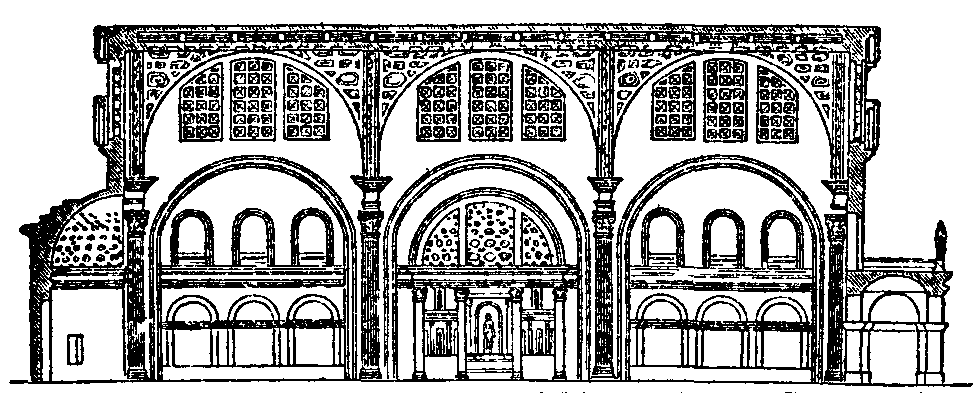
\includegraphics[width=5cm]{Basilica_5.png}}
\end{dispExample}

\begin{dispExample}
% \usepackage{tikz}
\tcbset{colframe=blue!50!black,colback=white,colupper=red!50!black,
        fonttitle=\bfseries,center title}

% Fixed width box
\begin{tcolorbox}Hello\\World!\end{tcolorbox}

% Fitted width box (like hbox or makebox)
\tcbox{Hello\\World!}

% Fitted width box (using a \tikzname\  node)
\tcbox[tikznode]{Hello\\World!}
\end{dispExample}

\end{docCommand}

\clearpage
\begin{marker}
See \Vref{subsec:xparse_tcolorbox} and \Vref{subsec:xparse_tcbox} for more
elaborate methods to create new environments and commands.
\end{marker}

\begin{docCommand}{newtcolorbox}{\oarg{init options}\marg{name}\oarg{number}\oarg{default}\marg{options}}
  Creates a new environment \meta{name} based on \refEnv{tcolorbox}.
  Basically, |\newtcolorbox| operates like |\newenvironment|. This means,
  the new environment \meta{name} optionally takes \meta{number} arguments, where
  \meta{default} is the default value for the optional first argument.
  The \meta{options} are given to the underlying |tcolorbox|.
  Note that \refKey{/tcb/savedelimiter} is set to the given \meta{name}
  automatically.
  The \meta{init options} allow setting up automatic numbering,
  see Section \ref{sec:initkeys} from page \pageref{sec:initkeys}.
\begin{dispExample*}{sbs,lefthand ratio=0.6}
\newtcolorbox{mybox}{colback=red!5!white,
  colframe=red!75!black}

\begin{mybox}
This is my own box.
\end{mybox}
\end{dispExample*}

\begin{dispExample*}{sbs,lefthand ratio=0.6}
\newtcolorbox{mybox}[1]{colback=red!5!white,
  colframe=red!75!black,fonttitle=\bfseries,
  title=#1}

\begin{mybox}{Hello there}
This is my own box with a mandatory title.
\end{mybox}
\end{dispExample*}

\begin{dispExample*}{sbs,lefthand ratio=0.6}
\newtcolorbox{mybox}[2][]{colback=red!5!white,
  colframe=red!75!black,fonttitle=\bfseries,
  colbacktitle=red!85!black,enhanced,
attach boxed title to top center={yshift=-2mm},
  title=#2,#1}

\begin{mybox}[colback=yellow]{Hello there}
This is my own box with a mandatory title
and options.
\end{mybox}
\end{dispExample*}

\inputpreamblelisting{A}

\begin{dispExample*}{sbs,lefthand ratio=0.6}
\begin{pabox}[colback=yellow]{Hello there}
This is my own box with a mandatory
numbered title and options.
\end{pabox}
\end{dispExample*}
\end{docCommand}


\begin{docCommand}{renewtcolorbox}{\oarg{init options}\marg{name}\oarg{number}\oarg{default}\marg{options}}
  Operates like \refCom{newtcolorbox}, but based on |\renewenvironment| instead of |\newenvironment|.
  An existing environment is redefined.
\end{docCommand}


\clearpage
\begin{docCommand}{newtcbox}{\oarg{init options}\brackets{\texttt{\textbackslash}\meta{name}}\oarg{number}\oarg{default}\marg{options}}
  Creates a new macro \texttt{\textbackslash}\meta{name} based on \refCom{tcbox}.
  Basically, |\newtcbox| operates like |\newcommand|.
  The new macro \texttt{\textbackslash}\meta{name} optionally takes \meta{number}$+1$ arguments, where
  \meta{default} is the default value for the optional first argument.
  The \meta{options} are given to the underlying |tcbox|.
  The \meta{init options} allow setting up automatic numbering,
  see Section \ref{sec:initkeys} from page \pageref{sec:initkeys}.
\begin{dispExample*}{sbs,lefthand ratio=0.6}
\newtcbox{\mybox}{colback=red!5!white,
  colframe=red!75!black}

\mybox{This is my own box.}
\end{dispExample*}

\begin{dispExample*}{sbs,lefthand ratio=0.6}
\newtcbox{\mybox}[1]{colback=red!5!white,
  colframe=red!75!black,fonttitle=\bfseries,
  title=#1}

\mybox{Hello there}{This is my own box.}
\end{dispExample*}

\begin{dispExample*}{sbs,lefthand ratio=0.6}
\newtcbox{\mybox}[2][]{colback=red!5!white,
  colframe=red!75!black,fonttitle=\bfseries,
  title=#2,#1}

\mybox[colback=yellow]{Hello there}%
  {This is my own box.}
\end{dispExample*}

\inputpreamblelisting{B}

\begin{dispExample*}{sbs,lefthand ratio=0.6}
\pbbox[colback=yellow]{Hello there}%
  {This is my own box.}
\end{dispExample*}

\begin{dispExample}
\newtcbox{\mybox}[1][red]{on line,
  arc=0pt,outer arc=0pt,colback=#1!10!white,colframe=#1!50!black,
  boxsep=0pt,left=1pt,right=1pt,top=2pt,bottom=2pt,
  boxrule=0pt,bottomrule=1pt,toprule=1pt}
\newtcbox{\xmybox}[1][red]{on line,
  arc=7pt,colback=#1!10!white,colframe=#1!50!black,
  before upper={\rule[-3pt]{0pt}{10pt}},boxrule=1pt,
  boxsep=0pt,left=6pt,right=6pt,top=2pt,bottom=2pt}

The \mybox[green]{quick} brown \mybox{fox} \mybox[blue]{jumps} over the
\mybox[green]{lazy} \mybox{dog}.\par
The \xmybox[green]{quick} brown \xmybox{fox} \xmybox[blue]{jumps} over the
\xmybox[green]{lazy} \xmybox{dog}.
\end{dispExample}

\end{docCommand}


\enlargethispage*{1cm}
\begin{docCommand}{renewtcbox}{\oarg{init options}\brackets{\texttt{\textbackslash}\rmfamily\meta{name}}\oarg{number}\oarg{default}\marg{options}}
  Operates like \refCom{newtcbox}, but based on |\renewcommand| instead of |\newcommand|.
  An existing macro is redefined.
\end{docCommand}



% !TeX root = tcolorbox.tex
% include file of tcolorbox.tex (manual of the LaTeX package tcolorbox)
\clearpage
\section{Option Keys}\label{sec:optkeys}%
\tcbset{external/prefix=external/coreoptions_}%
For the \meta{options} in \refEnv{tcolorbox} respectively \refCom{tcbset}
the following |pgf| keys can be applied. The key tree path |/tcb/| is not to
be used inside these macros. It is easy to add your own style keys using
the syntax for |pgf| keys, see \cite{tantau:2015a,sturm:2014g} or the examples
starting from page~\pageref{sec:latextutorial}.


\subsection{Title}
\begin{docTcbKey}{title}{=\meta{text}}{no default, initially empty}
  Creates a heading line with \meta{text} as content.
\begin{dispExample*}{sbs,lefthand ratio=0.6}
\begin{tcolorbox}[title=My heading line]
This is a \textbf{tcolorbox}.
\end{tcolorbox}
\end{dispExample*}
\end{docTcbKey}

\begin{docTcbKey}{notitle}{}{no value, initially set}
  Removes the title line if set before.
\end{docTcbKey}


\begin{docTcbKey}{adjusted title}{=\meta{text}}{style, no default, initially unset}
  Creates a heading line with \meta{text} as content. The minimal height of
  this line is adjusted to fit the text given by \refKey{/tcb/adjust text}.
  This option makes sense
  for single line headings if boxes are set side by side with equal height.
  Note that it is very easy to trick this adjustment.
\begin{exdispExample}[runs=2]{adjusted_title}
\tcbset{colback=White,arc=0mm,width=(\linewidth-4pt)/4,
equal height group=AT,before=,after=\hfill,fonttitle=\bfseries}

The following titles are not adjusted:\\
\foreach \n in {xxx,ggg,AAA,\"Agypten}
{\begin{tcolorbox}[title=\n,colframe=red!75!black]
  Some content.\end{tcolorbox}}
Now, we try again with adjusted titles:\\
\foreach \n in {xxx,ggg,AAA,\"Agypten}
{\begin{tcolorbox}[adjusted title=\n,colframe=blue!75!black]
  Some content.\end{tcolorbox}}
\end{exdispExample}
\end{docTcbKey}


\begin{docTcbKey}{adjust text}{=\meta{text}}{no default, initially \texttt{\"Apgjy}}
  This sets the reference text for \refKey{/tcb/adjusted title}. If your texts
  never exceed '\"Apgjy' in depth and height you don't need to care about this option.
\end{docTcbKey}

\clearpage

\begin{docTcbKey}[][doc new=2014-11-24]{squeezed title}{=\meta{text}}{style, no default, initially unset}
  Creates a single heading line with \meta{text} as content.
  If the \meta{text} is longer than the available space, the text is
  squeezed to fit into the available space.
\begin{dispExample}
% \tcbuselibrary{raster}
\begin{tcbitemize}[raster columns=3,raster equal height,
  colframe=red!75!black,colback=red!5!white,fonttitle=\bfseries]
\tcbitem[squeezed title={Short title}]
  First box
\tcbitem[squeezed title={This is a very very long title}]
  Second box
\tcbitem[squeezed title={This title is clearly to long for this application}]
  Third box
\end{tcbitemize}
\end{dispExample}
\end{docTcbKey}

\begin{docTcbKey}[][doc new=2014-11-24]{squeezed title*}{=\meta{text}}{style, no default, initially unset}
  This is a combination of \refKey{/tcb/adjusted title} and  \refKey{/tcb/squeezed title}.
\begin{dispExample}
% \tcbuselibrary{raster}
\begin{tcbitemize}[raster columns=3,raster equal height,
  colframe=red!75!black,colback=red!5!white,fonttitle=\bfseries]
\tcbitem[squeezed title*={Short title}]
  First box
\tcbitem[squeezed title*={This is a very very long title}]
  Second box
\tcbitem[squeezed title*={This title is clearly to long for this application}]
  Third box
\end{tcbitemize}
\end{dispExample}
\end{docTcbKey}

\clearpage
\begin{docTcbKey}{detach title}{}{no value}
Detaches the title from its normal position. The text of the title is
stored into \docAuxCommand{tcbtitletext} and the formatted title is
available by \docAuxCommand{tcbtitle}.
The main application is to move the title from its usual place to another one.
\begin{dispExample}
\newtcolorbox{mybox}[2][]{colbacktitle=red!10!white,
  colback=blue!10!white,coltitle=red!70!black,
  title={#2},fonttitle=\bfseries,#1}

\begin{mybox}{My title}
  This is a \textbf{tcolorbox}.
\end{mybox}
\begin{mybox}[detach title,before upper={\tcbtitle\quad}]{My title}
  This is a \textbf{tcolorbox}.
\end{mybox}
\begin{mybox}[detach title,after upper={\par\hfill\tcbtitle}]{My title}
  This is a \textbf{tcolorbox}.
\end{mybox}
\end{dispExample}
\end{docTcbKey}

\begin{docTcbKey}{attach title}{}{no value}
Attaches the title to its normal position. This option is used to reverse
\refKey{/tcb/detach title}.
\end{docTcbKey}


\begin{docTcbKey}[][doc updated=2015-07-08]{attach title to upper}{\colOpt{=\meta{text}}}{style, default empty, initially unset}
Attaches the title to the begin of the upper part of the box content.
The optional \meta{text} is set between the formatted title and the box content.
\begin{dispExample}
\newtcolorbox{mybox}[2][]{colbacktitle=red!10!white,
  colback=blue!10!white,coltitle=red!70!black,
  title={#2},fonttitle=\bfseries,#1}

\begin{mybox}[attach title to upper={\ ---\ }]{My title}
  This is a \textbf{tcolorbox}.
\end{mybox}
\begin{mybox}[attach title to upper,after title={:\ }]{My title}
  This is a \textbf{tcolorbox}.
\end{mybox}
\end{dispExample}
\end{docTcbKey}


\bigskip
\begin{marker}
More title options are documented in \Vref{subsec:contentadditions}
and \Vref{subsec:skinboxedtitle}.
\end{marker}

\clearpage
\subsection{Subtitle}

Inside the box content, one or more subtitles can be added.
In general, a subtitle is a further \refEnv{tcolorbox} which inherits some
color and geometry options from the enclosing box. It may be customized
just like any other \refEnv{tcolorbox}.

\begin{docCommand}[doc new=2014-10-10]{tcbsubtitle}{\oarg{options}\marg{text}}
  Used inside a \refEnv{tcolorbox} to add a subtitle box with the given \meta{text}.
  This is an independent \refEnv{tcolorbox} which is formatted by several
  inherited properties of the enclosing box, by further settings from
  \refKey{/tcb/subtitle style}, and by the given \meta{options}.
\begin{dispExample*}{sbs,lefthand ratio=0.6}
\begin{tcolorbox}[title=My title,
    colback=red!5!white,
    colframe=red!75!black,
    fonttitle=\bfseries]
  This is a \textbf{tcolorbox}.
\tcbsubtitle[before skip=\baselineskip]%
  {My subtitle}
  Further text.
\end{tcolorbox}
\end{dispExample*}
\begin{dispExample*}{sbs,lefthand ratio=0.6}
\begin{tcolorbox}[title=My title,
    colback=red!5!white,
    colframe=red!75!black,
    colbacktitle=yellow!50!red,
    coltitle=red!25!black,
    fonttitle=\bfseries]
  This is a \textbf{tcolorbox}.
\tcbsubtitle[before skip=\baselineskip]%
  {My subtitle}
  Further text.
\end{tcolorbox}
\end{dispExample*}
\end{docCommand}

\begin{docTcbKey}[][doc new=2014-10-10]{subtitle style}{=\meta{options}}{no default, initially empty}
  Adds |tcolorbox| \meta{options} to the settings for \refCom{tcbsubtitle}.
\begin{exdispExample*}{subtitle_style}{sbs,lefthand ratio=0.6}
\begin{tcolorbox}[title=My title,
  colback=red!5!white,
  colframe=red!75!black,
  colbacktitle=yellow!50!red,
  coltitle=red!25!black,
  fonttitle=\bfseries,
  subtitle style={boxrule=0.4pt,
    colback=yellow!50!red!25!white} ]
  This is a \textbf{tcolorbox}.
\tcbsubtitle{My subtitle}
  Further text.
\tcbsubtitle{Second subtitle}
  Further text.
\end{tcolorbox}
\end{exdispExample*}
\end{docTcbKey}

\clearpage
\subsection{Upper Part}
The text content of a \refEnv{tcolorbox} may be parted into a mandatory \emph{upper part}
and an optional \emph{lower part}. These parts are separated by
\refCom{tcblower}. If there is no \refCom{tcblower} present, there is no
\emph{lower part} and the \emph{upper part} forms the complete text content.

\begin{docTcbKey}[][doc new=2015-01-06]{upperbox}{=\meta{mode}}{no default, initially \texttt{visible}}
  Controls the treatment of the upper part of the box. If there is no lower part,
  this is the complete text content.
  Feasible values for \meta{mode} are:
  \begin{itemize}
  \item\docValue{visible}: usual type setting of the upper part,
  \item\docValue{invisible}: empty space instead of the upper part contents.
  \end{itemize}
\begin{exdispExample}{upperbox}
\begin{tcolorbox}[upperbox=invisible,colback=white]
This is a \textbf{tcolorbox} (but invisible).
\end{tcolorbox}

\bigskip

\begin{tcolorbox}[upperbox=invisible,colback=white]
This is a \textbf{tcolorbox} (but invisible).
\tcblower
This is the lower part.
\end{tcolorbox}
\end{exdispExample}
\end{docTcbKey}


\begin{docTcbKey}[][doc new=2015-01-06]{visible}{}{style, no value}
  Shortcut for setting \refKey{/tcb/upperbox} and \refKey{/tcb/lowerbox}
  to be \docValue{visible}.
\end{docTcbKey}

\begin{docTcbKey}[][doc new=2015-01-06]{invisible}{}{style, no value}
  Shortcut for setting \refKey{/tcb/upperbox} and \refKey{/tcb/lowerbox}
  to be \docValue{invisible}.
\begin{exdispExample}{invisible}
\begin{tcolorbox}[invisible]
This is a \textbf{tcolorbox} (but invisible).
\end{tcolorbox}
\end{exdispExample}
\end{docTcbKey}


\clearpage
\begin{docTcbKey}[][doc new=2015-05-04]{saveto}{=\meta{file name}}{no default, initially empty}
  Saves the content of the box into a file for an optional later usage.
  This is the counterpart of \refKey{/tcb/savelowerto}, but is saves not
  only the upper part but the whole content. If a lower part is present,
  it is also saved including \refCom{tcblower}.
  \begin{marker}
  This option cannot be combined with \refKey{/tcb/savelowerto}.
  \end{marker}

\begin{exdispExample}{saveto_1}
\begin{tcolorbox}[invisible,saveto=\jobname_mysave1.tex,colback=white]
This is a \textbf{tcolorbox} which seems to be empty.
The content is saved for later usage.
\end{tcolorbox}

Now, we load the saved text:\\
\input{\jobname_mysave1.tex}
\end{exdispExample}

\begin{exdispExample}{saveto_2}
\begin{tcolorbox}[saveto=\jobname_mysave2.tex]
This is a \textbf{tcolorbox}.
\tcblower
This is the lower part.
\end{tcolorbox}

Now, we load the saved text:
\begin{tcolorbox}[colframe=red,colback=red!10,
  coltitle=black,colbacktitle=red!20,sidebyside,
  title=Here we see the saved content including the lower part]
\input{\jobname_mysave2.tex}
\end{tcolorbox}
\end{exdispExample}
\end{docTcbKey}



\clearpage
\subsection{Lower Part}
\begin{docTcbKey}{lowerbox}{=\meta{mode}}{no default, initially \texttt{visible}}
  Controls the treatment of the lower part of the box.
  Feasible values for \meta{mode} are:
  \begin{itemize}
  \item\docValue{visible}: usual type setting of the lower part,
  \item\docValue{invisible}: empty space instead of the lower part contents,
  \item\docValue{ignored}: the lower part is not used (here).
  \end{itemize}
  The last two values are usually applied in connection with |savelowerto|.
\begin{exdispExample}{lowerbox}
\begin{tcolorbox}[lowerbox=invisible,colback=white]
This is a \textbf{tcolorbox}.
\tcblower
This is the lower part (but invisible).
\end{tcolorbox}

\begin{tcolorbox}[lowerbox=ignored,colback=white]
This is a \textbf{tcolorbox}.
\tcblower
This is the lower part (but ignored).
\end{tcolorbox}
\end{exdispExample}
\end{docTcbKey}


\begin{docTcbKey}[][doc updated=2014-11-28]{savelowerto}{=\meta{file name}}{no default, initially empty}
  Saves the content of the lower part into a file for an optional later usage.
\begin{exdispExample}{savelowerto}
\begin{tcolorbox}[lowerbox=invisible,savelowerto=\jobname_bspsave.tex,colback=white]
This is a \textbf{tcolorbox}.
\tcblower
This is the lower part which may be quite complex:
$\displaystyle f(x)=\frac{1+x^2}{1-x^2}$.
\end{tcolorbox}

Now, we load the saved text:\\
\input{\jobname_bspsave.tex}
\end{exdispExample}
\end{docTcbKey}

\clearpage
\begin{docTcbKey}{lower separated}{\colOpt{=true\textbar false}}{default |true|, initially |true|}
If set to |true|, the lower part is visually separated from the upper part.
It depends on the chosen skin how the visualization of the separation is done.
\enlargethispage*{1cm}
\begin{exdispExample}{lower_separated}
% \tcbuselibrary{skins,raster}
\begin{tcbraster}[colback=red!5!white,colframe=red!75!black,
  fonttitle=\bfseries,fontlower=\itshape]
%
\begin{tcolorbox}[title=Lower separated]
This is the upper part.
\tcblower
This is the lower part.
\end{tcolorbox}
%
\begin{tcolorbox}[title=Lower not separated,lower separated=false]
This is the upper part.
\tcblower
This is the lower part.
\end{tcolorbox}
%
\begin{tcolorbox}[sidebyside,title=Lower separated]
This is the upper part.
\tcblower
This is the lower part.
\end{tcolorbox}
%
\begin{tcolorbox}[sidebyside,title=Lower not separated,lower separated=false]
This is the upper part.
\tcblower
This is the lower part.
\end{tcolorbox}
%
\begin{tcolorbox}[beamer,title=Lower separated]
This is the upper part.
\tcblower
This is the lower part.
\end{tcolorbox}
%
\begin{tcolorbox}[beamer,title=Lower not separated,lower separated=false]
This is the upper part.
\tcblower
This is the lower part.
\end{tcolorbox}
%
\end{tcbraster}
\end{exdispExample}
\end{docTcbKey}


\clearpage
\begin{docTcbKey}{savedelimiter}{=\meta{name}}{no default, initially \texttt{tcolorbox}}
  Used in connection with new environment definitions which extend
  |tcolorbox| and use or allow the option |savelowerto|.
  To catch the end of the new box environment \meta{name} has to be the name of
  this environment. Additionally, the environment definition has to use
  |\tcolorbox| instead of
  |\begin{tcolorbox}| and |\endtcolorbox| instead of |\end{tcolorbox}|.
\begin{dispExample}
\newenvironment{mybox}[1]{%
  \tcolorbox[savedelimiter=mybox,
             savelowerto=\jobname_bspsave2.tex,lowerbox=ignored,
             colback=red!5!white,colframe=red!75!black,fonttitle=\bfseries,
             title=#1]}%
  {\endtcolorbox}

\begin{mybox}{My Example}
Upper part.
\tcblower
Saved lower part!
\end{mybox}

Now, the saved part is used:
\begin{tcolorbox}[colback=green!5]
\input{\jobname_bspsave2.tex}
\end{tcolorbox}
\end{dispExample}

The |savedelimiter| is used implicitely with \refCom{newtcolorbox} which
allows a more convenient usage:
\begin{dispExample}
\newtcolorbox{mybox}[1]{%
             savelowerto=\jobname_bspsave2.tex,lowerbox=ignored,
             colback=red!5!white,colframe=red!75!black,fonttitle=\bfseries,
             title=#1}%

\begin{mybox}{My Example}
Upper part.
\tcblower
Saved lower part!
\end{mybox}

Now, the saved part is used:
\begin{tcolorbox}[colback=green!5]
\input{\jobname_bspsave2.tex}
\end{tcolorbox}
\end{dispExample}
\end{docTcbKey}



\clearpage
\subsection{Colors and Fonts}
\begin{docTcbKey}{colframe}{=\meta{color}}{no default, initially \texttt{black!75!white}}
  Sets the frame \meta{color} of the box.
\begin{dispExample*}{sbs,lefthand ratio=0.6}
\begin{tcolorbox}[colframe=red!50!white]
This is a \textbf{tcolorbox}.
\end{tcolorbox}
\end{dispExample*}
\end{docTcbKey}

\begin{docTcbKey}{colback}{=\meta{color}}{no default, initially \texttt{black!5!white}}
  Sets the background \meta{color} of the box.
\begin{dispExample*}{sbs,lefthand ratio=0.6}
\begin{tcolorbox}[colback=red!50!white]
This is a \textbf{tcolorbox}.
\end{tcolorbox}
\end{dispExample*}
\end{docTcbKey}


\begin{docTcbKey}{title filled}{\colOpt{=true\textbar false}}{default |true|, initially |false|}
  Switches the drawing of the title background according to the given value.
  This option is set to |true| automatically by \refKey{/tcb/colbacktitle},
  \refKey{/tcb/opacitybacktitle}, and \refKey{/tcb/title style},
  and \refKey{/tcb/title code}.

\begin{dispExample*}{sbs,lefthand ratio=0.6}
\begin{tcolorbox}[title=My title,title filled]
This is a \textbf{tcolorbox}.
\end{tcolorbox}
\begin{tcolorbox}[title=My title,
  title filled=false]
This is a \textbf{tcolorbox}.
\end{tcolorbox}
\end{dispExample*}
\end{docTcbKey}


\begin{docTcbKey}{colbacktitle}{=\meta{color}}{no default, initially \texttt{black!50!white}}
  Sets the background \meta{color} of the title area of the box.
\begin{dispExample*}{sbs,lefthand ratio=0.6}
\begin{tcolorbox}[colbacktitle=red!50!white,
  title=My title,coltitle=black,
  fonttitle=\bfseries]
This is a \textbf{tcolorbox}.
\end{tcolorbox}
\end{dispExample*}
\end{docTcbKey}



\clearpage

\begin{docTcbKey}{colupper}{=\meta{color}}{no default, initially \texttt{black}}
  Sets the text \meta{color} of the upper part.
\begin{dispExample*}{sbs,lefthand ratio=0.6}
\begin{tcolorbox}[colupper=red!75!black]
This is a \textbf{tcolorbox}.
\tcblower
This is the lower part.
\end{tcolorbox}
\end{dispExample*}
\end{docTcbKey}


\begin{docTcbKey}{collower}{=\meta{color}}{no default, initially \texttt{black}}
  Sets the text \meta{color} of the lower part.
\begin{dispExample*}{sbs,lefthand ratio=0.6}
\begin{tcolorbox}[collower=red!75!black]
This is a \textbf{tcolorbox}.
\tcblower
This is the lower part.
\end{tcolorbox}
\end{dispExample*}
\end{docTcbKey}


\begin{docTcbKey}{coltext}{=\meta{color}}{style, no default, initially \texttt{black}}
  Sets the text \meta{color} of the box. This is an abbreviation for setting
  |colupper| and |collower| to the same value.
\begin{dispExample*}{sbs,lefthand ratio=0.6}
\begin{tcolorbox}[coltext=red!75!black]
This is a \textbf{tcolorbox}.
\tcblower
This is the lower part.
\end{tcolorbox}
\end{dispExample*}
\end{docTcbKey}


\begin{docTcbKey}{coltitle}{=\meta{color}}{no default, initially \texttt{white}}
  Sets the title text \meta{color} of the box.
\begin{dispExample*}{sbs,lefthand ratio=0.6}
\begin{tcolorbox}[coltitle=red!75!black,
  colbacktitle=black!10!white,title=Test]
This is a \textbf{tcolorbox}.
\end{tcolorbox}
\end{dispExample*}
\end{docTcbKey}

\clearpage

\begin{docTcbKey}{fontupper}{=\meta{text}}{no default, initially empty}
  Sets \meta{text} before the content of the upper part (e.\,g.\ font settings).
\begin{dispExample}
\begin{tcolorbox}[fontupper=Hello!~\sffamily]
This is a \textbf{tcolorbox}.
\end{tcolorbox}
\end{dispExample}
\end{docTcbKey}


\begin{docTcbKey}{fontlower}{=\meta{text}}{no default, initially empty}
  Sets \meta{text} before the content of the lower part (e.\,g.\ font settings).
\begin{dispExample}
\begin{tcolorbox}[fontlower=\sffamily\bfseries]
This is a \textbf{tcolorbox}.
\tcblower
This is the lower part.
\end{tcolorbox}
\end{dispExample}
\end{docTcbKey}


\begin{docTcbKey}{fonttitle}{=\meta{text}}{no default, initially empty}
  Sets \meta{text} before the content of the title text (e.\,g.\ font settings).
\begin{dispExample}
\begin{tcolorbox}[fonttitle=\sffamily\bfseries\large,title=Hello]
This is a \textbf{tcolorbox}.
\end{tcolorbox}
\end{dispExample}
\end{docTcbKey}

\bigskip
\begin{marker}
  More color options are provided by using skins documented in
  Section \ref{sec:skins} from page \pageref{sec:skins}.
\end{marker}


\clearpage
\subsection{Text Alignment}

\begin{docTcbKey}[][doc new=2015-05-07]{halign}{=\meta{alignment}}{no default, initially \texttt{justify}}
  If there is no lower part, |halign| determines the horizontal \meta{alignment}
  of the text content.
  Otherwise, |halign| determines the horizontal \meta{alignment}
  of the upper part of the box only.
  The feasible values for \meta{alignment} are more or less identical to
  the corresponding |/tikz/align| settings, even if the implementation differs.
  \begin{itemize}
  \item\docValue{justify}: usual left and right justified type setting.
  \item\docValue{left}: left border justification in analogy to plain \TeX.
  \item\docValue{flush left}: left border justification with |\raggedright| of \LaTeX.
  \item\docValue{right}: right border justification in analogy to plain \TeX.
  \item\docValue{flush right}: right border justification with |\raggedleft| of \LaTeX.
  \item\docValue{center}: centering in analogy to plain \TeX.
  \item\docValue{flush center}: centering with |\centering| of \LaTeX.
  \end{itemize}
  The differences between the flush and non-flush version are explained in
  detail in the \tikzname\ manual \cite{tantau:2015a}. The short story is that
  the non-flush versions will often look more balanced but with more
  hyphenations.

\begin{exdispExample}{halign}
\tcbset{colback=red!5!white,colframe=red!75!black,size=small,
  fonttitle=\bfseries,width=3.5cm,box align=top,
  nobeforeafter}

\begin{tcolorbox}[adjusted title=flush center,halign=flush center]
This is a demonstration text for showing how line breaking works.
\end{tcolorbox}
\begin{tcolorbox}[adjusted title=flush left,halign=flush left]
This is a demonstration text for showing how line breaking works.
\end{tcolorbox}
\begin{tcolorbox}[adjusted title=flush right,halign=flush right]
This is a demonstration text for showing how line breaking works.
\end{tcolorbox}

\begin{tcolorbox}[adjusted title=center,halign=center]
This is a demonstration text for showing how line breaking works.
\end{tcolorbox}
\begin{tcolorbox}[adjusted title=left,halign=left]
This is a demonstration text for showing how line breaking works.
\end{tcolorbox}
\begin{tcolorbox}[adjusted title=right,halign upper=right]
This is a demonstration text for showing how line breaking works.
\end{tcolorbox}
\end{exdispExample}

\end{docTcbKey}


\begin{docTcbKey}[][doc new=2015-05-07]{halign upper}{=\meta{alignment}}{no default, initially \texttt{justify}}
  Alias for \refKey{/tcb/halign}.
\end{docTcbKey}

\newpage
\begin{docTcbKey}[][doc new=2015-05-07]{halign lower}{=\meta{alignment}}{no default, initially \texttt{justify}}
  |halign lower| determines the horizontal \meta{alignment} of the lower part of the box.
  The feasible values for \meta{alignment} are the same as for \refKey{/tcb/halign}.

\begin{exdispExample}{halign_lower}
\begin{tcbraster}[raster columns=3,fonttitle=\bfseries,
  colback=red!5!white,colframe=red!75!black]

  \begin{tcolorbox}[adjusted title=flush center,halign lower=flush center]
    Upper part. \tcblower Lower part.
  \end{tcolorbox}
  \begin{tcolorbox}[adjusted title=flush left,halign lower=flush left]
    Upper part. \tcblower Lower part.
  \end{tcolorbox}
  \begin{tcolorbox}[adjusted title=flush right,halign lower=flush right]
    Upper part. \tcblower Lower part.
  \end{tcolorbox}
  \begin{tcolorbox}[adjusted title=center,halign lower=center]
    Upper part. \tcblower Lower part.
  \end{tcolorbox}
  \begin{tcolorbox}[adjusted title=left,halign lower=left]
    Upper part. \tcblower Lower part.
  \end{tcolorbox}
  \begin{tcolorbox}[adjusted title=right,halign lower=right]
    Upper part. \tcblower Lower part.
  \end{tcolorbox}

\end{tcbraster}
\end{exdispExample}
\end{docTcbKey}


\clearpage
\begin{docTcbKey}[][doc new=2015-05-07]{halign title}{=\meta{alignment}}{no default, initially \texttt{justify}}
  |halign lower| determines the horizontal \meta{alignment} of the title of the box.
  The feasible values for \meta{alignment} are the same as for \refKey{/tcb/halign}.

\begin{exdispExample}{halign_title}
\begin{tcbraster}[raster columns=3,fonttitle=\bfseries,
  colback=red!5!white,colframe=red!75!black]

  \begin{tcolorbox}[adjusted title=flush center,halign title=flush center]
    This is a \textbf{tcolorbox}.
  \end{tcolorbox}
  \begin{tcolorbox}[adjusted title=flush left,halign title=flush left]
    This is a \textbf{tcolorbox}.
  \end{tcolorbox}
  \begin{tcolorbox}[adjusted title=flush right,halign title=flush right]
    This is a \textbf{tcolorbox}.
  \end{tcolorbox}
  \begin{tcolorbox}[adjusted title=center,halign title=center]
    This is a \textbf{tcolorbox}.
  \end{tcolorbox}
  \begin{tcolorbox}[adjusted title=left,halign title=left]
    This is a \textbf{tcolorbox}.
  \end{tcolorbox}
  \begin{tcolorbox}[adjusted title=right,halign title=right]
    This is a \textbf{tcolorbox}.
  \end{tcolorbox}

\end{tcbraster}
\end{exdispExample}
\end{docTcbKey}

\enlargethispage*{1cm}

\begin{docTcbKey}[][doc updated=2015-05-07]{flushleft upper}{}{style, no value}
  Shortcut for setting \refKey{/tcb/halign} to \docValue{flush left}.
\end{docTcbKey}

\begin{docTcbKey}[][doc updated=2015-05-07]{center upper}{}{style, no value}
  Shortcut for setting \refKey{/tcb/halign} to \docValue{flush center}.
\end{docTcbKey}

\begin{docTcbKey}[][doc updated=2015-05-07]{flushright upper}{}{style, no value}
  Shortcut for setting \refKey{/tcb/halign} to \docValue{flush right}.
\end{docTcbKey}

\begin{docTcbKey}[][doc updated=2015-05-07]{flushleft lower}{}{style, no value}
  Shortcut for setting \refKey{/tcb/halign lower} to \docValue{flush left}.
\end{docTcbKey}

\begin{docTcbKey}[][doc updated=2015-05-07]{center lower}{}{style, no value}
  Shortcut for setting \refKey{/tcb/halign lower} to \docValue{flush center}.
\end{docTcbKey}

\begin{docTcbKey}[][doc updated=2015-05-07]{flushright lower}{}{style, no value}
  Shortcut for setting \refKey{/tcb/halign lower} to \docValue{flush right}.
\end{docTcbKey}


\begin{docTcbKey}[][doc updated=2015-05-07]{flushleft title}{}{style, no value}
  Shortcut for setting \refKey{/tcb/halign title} to \docValue{flush left}.
\end{docTcbKey}

\begin{docTcbKey}[][doc updated=2015-05-07]{center title}{}{style, no value}
  Shortcut for setting \refKey{/tcb/halign title} to \docValue{flush center}.
\end{docTcbKey}

\begin{docTcbKey}[][doc updated=2015-05-07]{flushright title}{}{style, no value}
  Shortcut for setting \refKey{/tcb/halign title} to \docValue{flush right}.
\end{docTcbKey}

\clearpage

\begin{marker}
The vertical alignment settings are only relevant for boxes which are larger
than their natural height, see \Fullref{sec:heightcontrol}.
\end{marker}

\begin{docTcbKey}[][doc updated=2015-07-16]{valign}{=\meta{alignment}}{no default, initially |top|}
  If the height of a |tcolorbox| is not the natural height, |valign|
  determines the vertical \meta{alignment} of the upper part.
  Feasible values are
  \begin{itemize}
  \item\docValue{top}: Anchor text at top.
  \item\docValue{center}: Anchor text at center.
  \item\docValue{bottom}: Anchor text at bottom.
  \item\docValue{scale}: Scale text vertically to fit into the available space.
    This is brutal and may not look very good. Consider \Fullref{sec:fitting}
    alternatively.
  \item\docValue{scale*}: Like \docValue{scale}, but scaling is bounded by
    \refKey{/tcb/valign scale limit}.
  \end{itemize}
  For a box with natural height, these settings are meaningless.
\begin{exdispExample}{valign}
\tcbset{width=(\linewidth-2mm)/4,before=,after=\hfill,
colframe=blue!75!black,colback=white,height=2cm}

\foreach \myalign in {top,center,bottom,scale}
{\begin{tcolorbox}[valign=\myalign]
  This is a \textbf{tcolorbox}.
\end{tcolorbox}}
\end{exdispExample}
\end{docTcbKey}


\begin{docTcbKey}[][doc new=2015-05-07]{valign upper}{=\meta{alignment}}{no default, initially \texttt{top}}
  Alias for \refKey{/tcb/valign}.
\end{docTcbKey}

\begin{docTcbKey}{valign lower}{=\meta{alignment}}{no default, initially |top|}
  This key has the same meaning for the lower part as |valign|
  for the upper part, i.\,e., it determines
  the vertical \meta{alignment} of the lower part with feasible values
  |top|, |center|, |bottom|, |scale|, and |scale*|.
\end{docTcbKey}

\begin{docTcbKey}[][doc new=2015-07-16]{valign scale limit}{=\meta{real number}}{no default, initially \texttt{1.1}}
  Sets an upper scale limit for the \docValue{scale*} setting in
  \refKey{/tcb/valign} and \refKey{/tcb/valign lower}.
  Note that this value is not reset by \refKey{/tcb/reset}. So, changes
  also apply to embedded boxes.
\end{docTcbKey}


Also see \refKey{/tcb/sidebyside align} for alignment settings when
upper part and lower part are set side-by-side.

\clearpage
\subsection{Geometry}
\subsubsection{Width}

\begin{docTcbKey}{width}{=\meta{length}}{no default, initially \cs{linewidth}}
  Sets the total width of the colored box to \meta{length}.
  See also \refKey{/tcb/height}.
\begin{dispExample}
\tcbset{colback=red!5!white,colframe=red!75!black}

\begin{tcolorbox}[width=\linewidth/2]
This is a \textbf{tcolorbox}.
\end{tcolorbox}
\end{dispExample}
\end{docTcbKey}


\begin{docTcbKey}[][doc new=2014-10-31]{text width}{=\meta{length}}{style, no default}
  Sets the text width of the upper part to \meta{length}.
  See also \refKey{/tcb/text height}.
\begin{dispExample}
\tcbset{colback=red!5!white,colframe=red!75!black}

\begin{tcolorbox}[text width=4cm]
This is a \textbf{tcolorbox} where the text has a width of 4cm.
\end{tcolorbox}
\end{dispExample}
\end{docTcbKey}

\begin{docTcbKey}[][doc new=2014-11-07]{add to width}{=\meta{length}}{style, no default}
  Adds \meta{length} to the current total width of the colored box.
\begin{dispExample*}{sbs,lefthand ratio=0.6}
\tcbset{width=4cm,colback=red!5!white,
  colframe=red!75!black}

\begin{tcolorbox}
This is a \textbf{tcolorbox}.
\end{tcolorbox}

\begin{tcolorbox}[add to width=1cm]
This is a \textbf{tcolorbox}.
\end{tcolorbox}
\end{dispExample*}
\end{docTcbKey}


See \Fullref{sec:heightcontrol} for setting fixed height values.


\clearpage
\subsubsection{Rules}
\begin{docTcbKey}{toprule}{=\meta{length}}{no default, initially \texttt{0.5mm}}
  Sets the line width of the top rule to \meta{length}.
\begin{dispExample}
\tcbset{colback=red!5!white,colframe=red!75!black}

\begin{tcolorbox}[toprule=3mm]
This is a \textbf{tcolorbox}.
\end{tcolorbox}
\end{dispExample}
\end{docTcbKey}


\begin{docTcbKey}{bottomrule}{=\meta{length}}{no default, initially \texttt{0.5mm}}
  Sets the line width of the bottom rule to \meta{length}.
\begin{dispExample}
\tcbset{colback=red!5!white,colframe=red!75!black}

\begin{tcolorbox}[bottomrule=3mm]
This is a \textbf{tcolorbox}.
\end{tcolorbox}
\end{dispExample}
\end{docTcbKey}

\begin{docTcbKey}{leftrule}{=\meta{length}}{no default, initially \texttt{0.5mm}}
  Sets the line width of the left rule to \meta{length}.
\begin{dispExample}
\tcbset{colback=red!5!white,colframe=red!75!black}

\begin{tcolorbox}[leftrule=3mm]
This is a \textbf{tcolorbox}.
\end{tcolorbox}
\end{dispExample}
\end{docTcbKey}


\begin{docTcbKey}{rightrule}{=\meta{length}}{no default, initially \texttt{0.5mm}}
  Sets the line width of the right rule to \meta{length}.
\begin{dispExample}
\tcbset{colback=red!5!white,colframe=red!75!black}

\begin{tcolorbox}[rightrule=3mm]
This is a \textbf{tcolorbox}.
\end{tcolorbox}
\end{dispExample}
\end{docTcbKey}

\clearpage
\begin{docTcbKey}{titlerule}{=\meta{length}}{no default, initially \texttt{0.5mm}}
  Sets the line width of the rule below the title to \meta{length}.
\begin{dispExample}
\tcbset{enhanced,colback=red!5!white,colframe=red!75!black,
  colbacktitle=red!90!black}

\begin{tcolorbox}[titlerule=3mm,title=This is the title]
This is a \textbf{tcolorbox}.
\end{tcolorbox}
\end{dispExample}
\end{docTcbKey}


\begin{docTcbKey}{boxrule}{=\meta{length}}{style, no default, initially \texttt{0.5mm}}
  Sets all rules of the frame to \meta{length}, i.\,e.\ 
  \refKey{/tcb/toprule}, \refKey{/tcb/bottomrule}, \refKey{/tcb/leftrule},
  \refKey{/tcb/rightrule}, and \refKey{/tcb/titlerule}.
\begin{dispExample}
\tcbset{colback=red!5!white,colframe=red!75!black}

\begin{tcolorbox}[boxrule=3mm]
This is a \textbf{tcolorbox}.
\end{tcolorbox}
\end{dispExample}
\end{docTcbKey}

\bigskip
\begin{marker}
  More options for drawing a \refKey{/tcb/borderline} are provided by using skins documented in
  Section \ref{sec:skins} from page \pageref{sec:skins}.
\end{marker}


\subsubsection{Arcs}
\begin{docTcbKey}{arc}{=\meta{length}}{no default, initially \texttt{1mm}}
  Sets the inner radius of the four frame arcs to \meta{length}.
\begin{exdispExample}{arc}
\tcbset{colback=red!5!white,colframe=red!75!black}

\begin{tcolorbox}[arc=0mm]
This is a \textbf{tcolorbox}.
\end{tcolorbox}
\begin{tcolorbox}[arc=3mm]
This is a \textbf{tcolorbox}.
\end{tcolorbox}
\end{exdispExample}
\end{docTcbKey}


\clearpage
\begin{docTcbKey}[][doc new=2015-05-05]{circular arc}{}{style, no value}
  Sets \refKey{/tcb/arc} to match the half of the inner width of the colored box.
  If width and height of the box are identical, this gives a circle.
  \begin{marker}
  If the height of the box is smaller than the width, the result will look
  quite ugly.
  \end{marker}
\begin{exdispExample*}{circular_arc}{sbs,lefthand ratio=0.6}
\begin{tcolorbox}[width=3cm,
  colback=red!5!white,
  colframe=red!75!black,
  halign=center,valign=center,
  square,circular arc]
This is a \textbf{tcolorbox}.
\end{tcolorbox}
\end{exdispExample*}
\end{docTcbKey}


\begin{docTcbKey}[][doc new=2015-05-05]{bean arc}{}{style, no value}
  Sets \refKey{/tcb/arc} to match the smaller value of the
  half of the inner width and of the inner height of the colored box.
  \begin{marker}
  This only works for a fixed \refKey{/tcb/height}. Also, \refKey{/tcb/bean arc}
  must be used \emph{after} width and height are set by option keys.
  \end{marker}
\begin{exdispExample*}{bean_arc}{sbs,lefthand ratio=0.6}
\tcbset{size=fbox,boxrule=0.5mm,
  colback=red!5!white,
  colframe=red!75!black,
  halign=center,valign=center}

\begin{tcolorbox}[width=3cm,height=2cm,
  bean arc]
Box A
\end{tcolorbox}

\begin{tcolorbox}[width=2cm,height=3cm,
  bean arc]
Box B
\end{tcolorbox}
\end{exdispExample*}
\end{docTcbKey}

\begin{docTcbKey}[][doc new=2015-05-05]{octogon arc}{}{style, no value}
  Sets \refKey{/tcb/arc} to match $\frac{1}{2+\sqrt{2}}$ of the inner width
  of the colored box. If width and height of the box are identical,
  the interior is a regular octogon.
\begin{exdispExample*}{octogon_arc}{sbs,lefthand ratio=0.8}
\begin{tcolorbox}[enhanced,
  size=minimal,auto outer arc,
  width=2.1cm,octogon arc,
  colback=red,colframe=white,colupper=white,
  fontupper=\fontsize{7mm}{7mm}\selectfont\bfseries\sffamily,
  halign=center,valign=center,
  square,arc is angular,
  borderline={0.2mm}{-1mm}{red}  ]
STOP
\end{tcolorbox}
\end{exdispExample*}
\end{docTcbKey}

\clearpage
\begin{docTcbKey}[][doc new=2015-05-05]{arc is angular}{}{no value, initially unset}
  Using this options applies a patch which straightens the corners arcs of
  the boxes. The little arcs are replaced by little straight lines.
  \begin{marker}
  This patch is considered as an experimental feature.
  It changes some of the original \tikzname\ code. This change may break
  with future updates of \tikzname.
  \end{marker}

\begin{exdispExample*}{arc_is_angular}{sbs,lefthand ratio=0.6}
\tcbset{colback=red!5!white,colframe=red!75!black,
  arc=3mm}

\begin{tcolorbox}[arc is angular]
This is a \textbf{tcolorbox}.
\end{tcolorbox}
\begin{tcolorbox}[arc is curved]
This is a \textbf{tcolorbox}.
\end{tcolorbox}
\end{exdispExample*}

\end{docTcbKey}


\begin{docTcbKey}[][doc new=2015-05-05]{arc is curved}{}{no value, initially set}
  This option resets the patch from \refKey{/tcb/arc is angular}. The
  original \tikzname\ code is activated.
\end{docTcbKey}


\begin{docTcbKey}{outer arc}{=\meta{length}}{no default, initially unset}
  Sets the outer radius of the four frame arcs to \meta{length}.
\begin{dispExample}
\tcbset{colback=red!5!white,colframe=red!75!black}

\begin{tcolorbox}[arc=4mm,outer arc=1mm]
This is a \textbf{tcolorbox}.
\end{tcolorbox}
\end{dispExample}
\end{docTcbKey}


\begin{docTcbKey}{auto outer arc}{}{no value, initially set}
  Sets the outer radius of the four frame arcs automatically in
  dependency of the inner radius given by \refKey{/tcb/arc}.
\end{docTcbKey}


\subsubsection{Spacing}\enlargethispage*{2cm}
\begin{docTcbKey}{boxsep}{=\meta{length}}{no default, initially \texttt{1mm}}
  Sets a common padding of \meta{length} between the text content and the
  frame of the box. This value is added to the key values of
  |left|, |right|, |top|, |bottom|, and |middle| at the appropriate places.
\begin{dispExample}
\tcbset{colback=red!5!white,colframe=red!75!black,width=(\linewidth-4mm)/2,
  before=,after=\hfill}

\begin{tcolorbox}[boxsep=5mm]
This is a \textbf{tcolorbox}.
\end{tcolorbox}
\begin{tcolorbox}[boxsep=5mm,draft]
This is a \textbf{tcolorbox}.
\end{tcolorbox}
\end{dispExample}
\end{docTcbKey}

\clearpage


\begin{docTcbKey}{left}{=\meta{length}}{style, no default, initially \texttt{4mm}}
  Sets the left space between all text parts and frame (additional to |boxsep|).
  This is an abbreviation for setting
  |lefttitle|, |leftupper|, and |leftlower| to the same value.
\begin{dispExample}
\tcbset{colback=red!5!white,colframe=red!75!black}

\begin{tcolorbox}[left=0mm]
This is a \textbf{tcolorbox}.
\end{tcolorbox}
\end{dispExample}
\end{docTcbKey}

\begin{docTcbKey}{lefttitle}{=\meta{length}}{no default, initially \texttt{4mm}}
  Sets the left space between title text and frame (additional to |boxsep|).
\begin{dispExample}
\tcbset{colback=red!5!white,colframe=red!75!black}

\begin{tcolorbox}[lefttitle=3cm,title=My Title]
This is a \textbf{tcolorbox}.
\end{tcolorbox}
\end{dispExample}
\end{docTcbKey}


\begin{docTcbKey}{leftupper}{=\meta{length}}{no default, initially \texttt{4mm}}
  Sets the left space between upper text and frame (additional to |boxsep|).
\begin{dispExample}
\tcbset{colback=red!5!white,colframe=red!75!black}

\begin{tcolorbox}[leftupper=3cm,title=My Title]
This is a \textbf{tcolorbox}.
\end{tcolorbox}
\end{dispExample}
\end{docTcbKey}

\begin{docTcbKey}{leftlower}{=\meta{length}}{no default, initially \texttt{4mm}}
  Sets the left space between lower text and frame (additional to |boxsep|).
\begin{dispExample}
\tcbset{colback=red!5!white,colframe=red!75!black}

\begin{tcolorbox}[leftlower=3cm]
This is a \textbf{tcolorbox}.
\tcblower
This is the lower part.
\end{tcolorbox}
\end{dispExample}
\end{docTcbKey}


\clearpage
\begin{docTcbKey}{right}{=\meta{length}}{style, no default, initially \texttt{4mm}}
  Sets the right space between all text parts and frame (additional to |boxsep|).
  This is an abbreviation for setting
  |righttitle|, |rightupper|, and |rightlower| to the same value.
\begin{dispExample}
\tcbset{colback=red!5!white,colframe=red!75!black}

\begin{tcolorbox}[width=5cm,right=2cm]
This is a \textbf{tcolorbox}.
\end{tcolorbox}
\end{dispExample}
\end{docTcbKey}



\begin{docTcbKey}{righttitle}{=\meta{length}}{no default, initially \texttt{4mm}}
  Sets the right space between title text and frame (additional to |boxsep|).
\begin{dispExample}
\tcbset{colback=red!5!white,colframe=red!75!black}

\begin{tcolorbox}[width=5cm,righttitle=2cm,title=My very long title text]
This is a \textbf{tcolorbox} with standard upper box dimensions.
\end{tcolorbox}
\end{dispExample}
\end{docTcbKey}


\begin{docTcbKey}{rightupper}{=\meta{length}}{no default, initially \texttt{4mm}}
  Sets the right space between upper text and frame (additional to |boxsep|).
\begin{dispExample}
\tcbset{colback=red!5!white,colframe=red!75!black}

\begin{tcolorbox}[width=5cm,rightupper=2cm,title=My very long title text]
This is a \textbf{tcolorbox} with compressed upper box dimensions.
\end{tcolorbox}
\end{dispExample}
\end{docTcbKey}


\clearpage
\begin{docTcbKey}{rightlower}{=\meta{length}}{no default, initially \texttt{4mm}}
  Sets the right space between lower text and frame (additional to |boxsep|).
\begin{dispExample}
\tcbset{colback=red!5!white,colframe=red!75!black}

\begin{tcolorbox}[width=5cm,rightlower=2cm]
This is a \textbf{tcolorbox} with standard upper box dimensions.
\tcblower
This is the lower part with large space at right.
\end{tcolorbox}
\end{dispExample}
\end{docTcbKey}



\begin{docTcbKey}{top}{=\meta{length}}{no default, initially \texttt{2mm}}
  Sets the top space between text and frame (additional to |boxsep|).
\begin{dispExample}
\tcbset{colback=red!5!white,colframe=red!75!black}

\begin{tcolorbox}[top=0mm]
This is a \textbf{tcolorbox}.
\tcblower
This is the lower part.
\end{tcolorbox}
\end{dispExample}
\end{docTcbKey}


\begin{docTcbKey}{toptitle}{=\meta{length}}{no default, initially \texttt{0mm}}
  Sets the top space between title and frame (additional to |boxsep|).
\begin{dispExample}
\tcbset{colback=red!5!white,colframe=red!75!black}

\begin{tcolorbox}[toptitle=3mm,title=My title]
This is a \textbf{tcolorbox}.
\end{tcolorbox}
\end{dispExample}
\end{docTcbKey}

\clearpage
\begin{docTcbKey}{bottom}{=\meta{length}}{no default, initially \texttt{2mm}}
  Sets the bottom space between text and frame (additional to |boxsep|).
\begin{dispExample}
\tcbset{colback=red!5!white,colframe=red!75!black}

\begin{tcolorbox}[bottom=0mm]
This is a \textbf{tcolorbox}.
\tcblower
This is the lower part.
\end{tcolorbox}
\end{dispExample}
\end{docTcbKey}

\begin{docTcbKey}{bottomtitle}{=\meta{length}}{no default, initially \texttt{0mm}}
  Sets the bottom space between title and frame (additional to |boxsep|).
\begin{dispExample}
\tcbset{colback=red!5!white,colframe=red!75!black}

\begin{tcolorbox}[bottomtitle=3mm,title=My title]
This is a \textbf{tcolorbox}.
\end{tcolorbox}
\end{dispExample}
\end{docTcbKey}


\begin{docTcbKey}{middle}{=\meta{length}}{no default, initially \texttt{2mm}}
  Sets the space between upper and lower text to the separation line
  (additional to |boxsep|).
\begin{dispExample}
\tcbset{colback=red!5!white,colframe=red!75!black}

\begin{tcolorbox}[middle=0mm,boxsep=0mm]
This is a \textbf{tcolorbox}.
\tcblower
This is the lower part.
\end{tcolorbox}
\end{dispExample}
\end{docTcbKey}

\clearpage
\subsubsection{Size Shortcuts}
\begin{docTcbKey}{size}{=\meta{name}}{no default, initially \texttt{normal}}
  Sets all geometry keys with exception of \refKey{/tcb/width} to
  predefined length values.
  For \meta{name}, the following values are feasible:
  \begin{itemize}
  \item\docValue{normal}: normal sized boxes e.g. of width |\linewidth|.
  \item\docValue{title}: title line sized boxes.
  \item\docValue{small}: small boxes e.g. for keyword highlighting.
  \item\docValue{fbox}: identical to the standard |\fbox|.
  \item\docValue{tight}: no padding space at all.
  \item\docValue{minimal}: no padding space, no box rules.
  \end{itemize}

\begin{dispExample}
\tcbset{colback=red!5!white,colframe=red!75!black}

\foreach \s in {minimal,tight,fbox,small,title,normal} {
  \tcbox[size=\s,on line]{\s} }

\foreach \s in {minimal,tight,fbox,small,title,normal} {
  \tcbox[size=\s,on line,title=Test]{\s} }

\foreach \s in {minimal,tight,fbox,small,title,normal} {
  \begin{tcolorbox}[size=\s,on line,title=Test,width=2.2cm]
    \s \tcblower lower\end{tcolorbox} }
\end{dispExample}

\bigskip

\begin{tcolorbox}[tabularx={l|XXXXXX},title=Predefined values,
enhanced,fonttitle=\small\bfseries,fontupper=\small\ttfamily,
colback=yellow!10!white,colframe=red!50!black,colbacktitle=Salmon!30!white,
coltitle=black,center title
]
            & normal & title  & small & fbox  & tight & minimal\\\hline
boxrule     & 0.5mm  & 0.4mm  & 0.3mm & 0.4pt & 0.4pt & 0.0pt \\
boxsep      & 1.0mm  & 1.0mm  & 1.0mm & 3.0pt & 0.0pt & 0.0pt \\
left        & 4.0mm  & 2.0mm  & 1.0mm & 0.0pt & 0.0pt & 0.0pt \\
right       & 4.0mm  & 2.0mm  & 1.0mm & 0.0pt & 0.0pt & 0.0pt \\
top         & 2.0mm  & 0.25mm & 0.0mm & 0.0pt & 0.0pt & 0.0pt \\
bottom      & 2.0mm  & 0.25mm & 0.0mm & 0.0pt & 0.0pt & 0.0pt \\
toptitle    & 0.0mm  & 0.0mm  & 0.0mm & 0.0pt & 0.0pt & 0.0pt \\
bottomtitle & 0.0mm  & 0.0mm  & 0.0mm & 0.0pt & 0.0pt & 0.0pt \\
middle      & 2.0mm  & 0.75mm & 0.5mm & 1.0pt & 0.2pt & 0.0pt \\
arc         & 1.0mm  & 0.75mm & 0.5mm & 1.0pt & 0.0pt & 0.0pt \\
outer arc   & auto   & auto   & auto  & auto  & 0.0pt & 0.0pt \\
\end{tcolorbox}
\end{docTcbKey}


\clearpage
\begin{docTcbKey}{oversize}{\colOpt{=\meta{length}}}{style, default |0pt|}
  Sets the text width of the upper part to the current line width plus an
  optional \meta{length}.
  This is achieved by changing the keys \refKey{/tcb/width}
  \refKey{/tcb/enlarge left by}, and
  \refKey{/tcb/enlarge right by} appropriately.
  The resulting box is overlapping into the left and right margin of
  the page.
  Note that this style option has to be given \emph{after} all other
  geometry keys!
\begin{dispListing}
\tcbset{colback=red!5!white,colframe=red!75!black,fonttitle=\bfseries}

\textit{Normal text for comparison:}\\
\lipsum[2]

\begin{tcolorbox}[oversize,title=Oversized box]
\lipsum[2]
\end{tcolorbox}

\begin{tcolorbox}[title=Normal box]
\lipsum[2]
\end{tcolorbox}
\end{dispListing}
\end{docTcbKey}

{\tcbusetemp}


\clearpage
\begin{docTcbKey}[][doc updated=2015-11-13]{toggle left and right}{=\meta{toggle preset}}{default |evenpage|, initially |none|}
  According to the \meta{toggle preset}, the left and the right settings of
  the |tcolorbox| are switched or not. Feasible values are:
  \begin{itemize}
  \item\docValue{none}: no switching.
  \item\docValue{forced}: the values of the left and right rules and spaces are switched.
  \item\docValue{evenpage}: if the page is an even page, the values of the left and
    right rules and spaces are switched. This value also sets
    \refKey{/tcb/check odd page} to |true|.
  \end{itemize}
\begin{marker}
Horizontal bounding box enlargements are not toggled by this option.
They can be toggled independently by \refKey{/tcb/toggle enlargement}.
For example, \refKey{/tcb/oversize} changes the bounding box.
\end{marker}
\begin{dispListing}
% \usepackage{lipsum}
% \usetikzlibrary{patterns}
% \tcbuselibrary{skins,breakable}
\begin{tcolorbox}[skin=enhancedmiddle,breakable,
  toggle left and right,
  boxrule=0mm,top=0mm,bottom=0mm,left=1mm,right=1mm,
  rightrule=1cm,colupper=blue!25!black,
  interior style={fill overzoom image=lichtspiel.jpg,fill image opacity=0.25},
  frame style={pattern=crosshatch dots light steel blue},
  overlay={%
    \tcbifoddpage{\coordinate (X) at ([xshift=-5mm]frame.east);}
                 {\coordinate (X) at ([xshift=5mm]frame.west);}
    \fill[shading=ball,ball color=blue!50!white,opacity=0.5] (X) circle (4mm);}]
\lipsum[1-6]
\end{tcolorbox}
\end{dispListing}
\medskip

This example switches a |1cm| thick rule from the left to the right side
depending on the page number. Thereby, the rule is always on the outer side
of the double-sided paper. Additionally, a ball is drawn on the outer side
with help of an overlay.
\bigskip

\tcbusetemp
\end{docTcbKey}

\clearpage
\subsection{Corners}\label{subsec:corners}

The four corners of any |tcolorbox| can be set individually as
\refKey{/tcb/sharp corners} or as \refKey{/tcb/rounded corners}.
These settings are also reflected in the behavior of \refKey{/tcb/borderline}
and \refKey{/tcb/shadow} as one would expect.

By default, all four corners are \emph{rounded}. So, only the
\refKey{/tcb/sharp corners} option will be necessary for most use cases.
The \refKey{/tcb/rounded corners} option can be used to revert a \refKey{/tcb/sharp corners}
setting.

\begin{docTcbKey}{sharp corners}{=\meta{position}}{default |all|, initially unset}
The \meta{position} denotes one or more of the four box corners to be set as
\emph{sharp} corners. The not assigned corners will retain their mode.
Feasible values for \meta{position} are:
\begin{itemize}
\foreach \p in {northwest,northeast,southwest,southeast,north,south,east,west,downhill,uphill,all}
{
\item\tcbox[on line,size=title,arc=2mm,colframe=red!75!black,colback=red!5!white,
  enlarge top by=0.5mm,enlarge bottom by=0.5mm,sharp corners=\p]{\docValue{\p}}
}
\end{itemize}
\begin{dispExample*}{sbs,lefthand ratio=0.6}
\begin{tcolorbox}[colback=red!5!white,
  colframe=red!75!black,
  sharp corners=northwest ]
This is a \textbf{tcolorbox}.
\end{tcolorbox}
\end{dispExample*}
\begin{dispExample*}{sbs,lefthand ratio=0.6}
\begin{tcolorbox}[colback=red!5!white,
  colframe=red!75!black,
  sharp corners ]
This is a \textbf{tcolorbox}.
\end{tcolorbox}
\end{dispExample*}
\end{docTcbKey}

\clearpage
\begin{docTcbKey}{rounded corners}{=\meta{position}}{default |all|, initially |all|}
The \refKey{/tcb/rounded corners} can be used to revert a \refKey{/tcb/sharp corners}
setting. The \meta{position} denotes one or more of the four box corners to be set as
\emph{rounded} corners. The not assigned corners will retain their mode.
Feasible values for \meta{position} are\footnote{The graphical examples assume
  that the boxes where set to have sharp corners before.}:
\begin{itemize}
\foreach \p in {northwest,northeast,southwest,southeast,north,south,east,west,downhill,uphill,all}
{
\item\tcbox[on line,size=title,arc=2mm,colframe=red!75!black,colback=red!5!white,
  enlarge top by=0.5mm,enlarge bottom by=0.5mm,sharp corners,rounded corners=\p]{\docValue{\p}}
}
\end{itemize}
\begin{dispExample*}{sbs,lefthand ratio=0.6}
\begin{tcolorbox}[colback=red!5!white,
  colframe=red!75!black,sharp corners,
  rounded corners=northwest ]
This is a \textbf{tcolorbox}.
\end{tcolorbox}
\end{dispExample*}
\end{docTcbKey}


\begin{docTcbKey}{sharpish corners}{}{style, no value}
  Shortcut for setting \refKey{/tcb/arc} and \refKey{/tcb/outer arc}
  to |0pt|. With this setting, rounded corners will appear as quasi-sharp,
  but e.\,g.\ the shadow will be somewhat rounder than the shadow
  of really sharp corners.
  \begin{marker}
  Corners are still of type \emph{rounded} with this option, but appear
  \emph{sharp}. To switch back to rounded corners, one has to adapt
  \refKey{/tcb/arc} and \refKey{/tcb/outer arc}.
  \end{marker}
\begin{dispExample*}{sbs,lefthand ratio=0.6}
\begin{tcolorbox}[colback=red!5!white,
  colframe=red!75!black,
  sharpish corners ]
This is a \textbf{tcolorbox}.
\end{tcolorbox}
\end{dispExample*}
\end{docTcbKey}

\clearpage

The following examples will show the differences between
\refKey{/tcb/rounded corners}, \refKey{/tcb/sharpish corners}, and \refKey{/tcb/sharp corners}.
The later two give the same core box, but \refKey{/tcb/borderline}
and \refKey{/tcb/shadow} settings are slightly different.
The following examples use \refKey{/tcb/drop fuzzy shadow}.

\foreach \n in {rounded corners,sharpish corners,sharp corners}{
\begin{tcolorbox}[enhanced jigsaw,frame empty,interior empty,fuzzy halo,halign=center]
\begin{tcolorbox}[enhanced,drop fuzzy shadow,width=\linewidth-1cm,
  colback=red!5!white, colframe=red!75!black, fonttitle=\bfseries,
  title=My title,\n,
  tikz={spy using outlines={circle, magnification=8, size=2cm, connect spies}},
  overlay={\spy [blue, size=4cm] on (frame.south east)
      in node at ([xshift=-2.5cm,yshift=-2.5cm]frame.south east);
  \node[right] at ([xshift=2cm,yshift=-1cm]frame.south west) {\textbf{\Large\ttfamily\n}};
  }]
This is a \textbf{tcolorbox}.
\end{tcolorbox}
\end{tcolorbox}}


\clearpage
\subsection{Transparency}

\begin{marker}
Transparency effects are likely to be used in conjunction with \emph{jigsaw}
skin variants, see \Vref{subsec:skinjigsaw}.
\end{marker}

\begin{docTcbKey}{opacityframe}{=\meta{fraction}}{no default, initially \texttt{1.0}}
  Sets the frame opacity of the box to the given \meta{fraction}.
\begin{exdispExample*}{opacityframe}{sbs,lefthand ratio=0.6,segmentation style={pattern=checkerboard light gray}}
\begin{tcolorbox}[opacityframe=0.25,
  colframe=red]
This is a \textbf{tcolorbox}.
\end{tcolorbox}
\end{exdispExample*}
\end{docTcbKey}

\begin{docTcbKey}{opacityback}{=\meta{fraction}}{no default, initially \texttt{1.0}}
  Sets the background opacity of the box to the given \meta{fraction}.
\begin{exdispExample*}{opacityback}{sbs,lefthand ratio=0.6,segmentation style={pattern=checkerboard light gray}}
\begin{tcolorbox}[standard jigsaw,colframe=red,
  opacityframe=0.5, opacityback=0.5]
This is a \textbf{tcolorbox}.
\end{tcolorbox}
\end{exdispExample*}
\end{docTcbKey}


\begin{docTcbKey}{opacitybacktitle}{=\meta{fraction}}{no default, initially \texttt{1.0}}
  Sets the title background opacity of the box to the given \meta{fraction}.
\begin{exdispExample*}{opacitybacktitle}{sbs,lefthand ratio=0.6,segmentation style={pattern=checkerboard light gray}}
\begin{tcolorbox}[standard jigsaw,colframe=red,
  opacityframe=0.5, opacitybacktitle=0.5,
  title filled, title=This is a title]
This is a \textbf{tcolorbox}.
\end{tcolorbox}
\end{exdispExample*}
\end{docTcbKey}


\begin{docTcbKey}{opacityfill}{=\meta{fraction}}{style, no default, initially \texttt{1.0}}
  Sets the fill opacity for frame, interior and optionally the title background
  to the given \meta{fraction}.
\begin{exdispExample*}{opacityfill}{sbs,lefthand ratio=0.6,segmentation style={pattern=checkerboard light gray}}
\begin{tcolorbox}[standard jigsaw,colframe=red,
  opacityfill=0.7, title=This is a title]
This is a \textbf{tcolorbox}.
\end{tcolorbox}
\end{exdispExample*}
\end{docTcbKey}

\clearpage
\begin{docTcbKey}{opacityupper}{=\meta{fraction}}{no default, initially \texttt{1.0}}
  Sets the text opacity of the upper box part to the given \meta{fraction}.
\begin{exdispExample*}{opacityupper}{sbs,lefthand ratio=0.6}
\begin{tcolorbox}[enhanced,opacityupper=0.5,
  interior style={pattern=checkerboard light gray}]
This is a \textbf{tcolorbox}.
\end{tcolorbox}
\end{exdispExample*}
\end{docTcbKey}


\begin{docTcbKey}{opacitylower}{=\meta{fraction}}{no default, initially \texttt{1.0}}
  Sets the text opacity of the lower box part to the given \meta{fraction}.
\begin{exdispExample*}{opacitylower}{sbs,lefthand ratio=0.6}
\begin{tcolorbox}[enhanced,opacitylower=0.5,
  interior style={pattern=checkerboard light gray}]
This is a \textbf{tcolorbox}.
\tcblower
This is the lower part.
\end{tcolorbox}
\end{exdispExample*}
\end{docTcbKey}

\begin{docTcbKey}{opacitytext}{=\meta{fraction}}{no default, initially \texttt{1.0}}
  Sets the text opacity of the upper and the lower box part to the given \meta{fraction}.
\begin{exdispExample*}{opacitytext}{sbs,lefthand ratio=0.6}
\begin{tcolorbox}[enhanced,opacitytext=0.5,
  interior style={pattern=checkerboard light gray}]
This is a \textbf{tcolorbox}.
\tcblower
This is the lower part.
\end{tcolorbox}
\end{exdispExample*}
\end{docTcbKey}


\begin{docTcbKey}{opacitytitle}{=\meta{fraction}}{no default, initially \texttt{1.0}}
  Sets the text opacity of the box title to the given \meta{fraction}.
\begin{exdispExample*}{opacitytitle}{sbs,lefthand ratio=0.6}
\begin{tcolorbox}[enhanced,opacitytitle=0.7,
  coltitle=black,
  fonttitle=\bfseries,title=This is a title,
  title style={pattern=checkerboard light gray}]
This is a \textbf{tcolorbox}.
\end{tcolorbox}
\end{exdispExample*}
\end{docTcbKey}


\begin{exdispExample*}{opacity_general}{segmentation style={pattern=checkerboard light gray}}
\begin{tcolorbox}[enhanced jigsaw,fonttitle=\bfseries,title=This is a title,
  opacityframe=0.5,opacityback=0.25,opacitybacktitle=0.25,opacitytext=0.8,
  colback=red!5!white,colframe=red!75!black,colbacktitle=yellow!20!red]
This is a \textbf{tcolorbox}.
\end{tcolorbox}
\end{exdispExample*}



\clearpage
\subsection{Height Control}\label{sec:heightcontrol}
In a typical usage scenario, the height of a |tcolorbox| is computed automatically
to fit the content. Nevertheless, the height can be set to a fixed value
or to fit commonly for several boxes, e.\,g. if boxes are set side by side.

\bigskip
\begin{marker}
  The height control keys are only applicable to unbreakable boxes.
  If a box is set to be \refKey{/tcb/breakable}, the height is always
  computed according to the \emph{natural height}.
\end{marker}
\bigskip


\begin{docTcbKey}{natural height}{}{no value, initially set}
  Sets the total height of the colored box to its natural height depending
  on the box content.
\end{docTcbKey}

\begin{docTcbKey}{height}{=\meta{length}}{no default}
  Sets the total height of the colored box to \meta{length} independent
  of the box content. \meta{length} is the minimum height of the box, if
  \refKey{/tcb/height plus} is larger than zero.
\begin{dispExample}
\tcbset{width=(\linewidth-2mm)/3,before=,after=\hfill,
colframe=blue!75!black,colback=white}

\begin{tcolorbox}[height=1cm,valign=center]
  This box has a height of 1cm.
\end{tcolorbox}
\begin{tcolorbox}[height=2cm,valign=center]
  This box has a height of 2cm.
\end{tcolorbox}
\begin{tcolorbox}[height=3cm,split=0.5,valign=center,valign lower=center]
  This box has a height of 3cm.
  \tcblower
  Lower part.
\end{tcolorbox}
\end{dispExample}
\end{docTcbKey}

\enlargethispage*{10mm}
\begin{docTcbKey}{height plus}{=\meta{length}}{no default, initially |0pt|}
  The box may extend a given fixed \refKey{/tcb/height} up to the given \meta{length}.
\begin{dispExample}
\tcbset{colback=red!5!white,colframe=red!75!black,left=1mm,top=1mm,bottom=1mm,
  right=1mm,boxsep=0mm,width=3cm,nobeforeafter}

\begin{tcolorbox}[height=1cm]
This is a tcolorbox.
\end{tcolorbox}
\begin{tcolorbox}[height=1cm,height plus=1cm]
This is a tcolorbox.
\end{tcolorbox}
\begin{tcolorbox}[height=1cm,height plus=1cm]
This is a tcolorbox. This is a tcolorbox. This is a tcolorbox.
\end{tcolorbox}
\end{dispExample}
\end{docTcbKey}


\begin{docTcbKey}{height from}{=\meta{min} \texttt{to} \meta{max}}{style, no default}
  Sets the box height to a dimension between \meta{min} and \meta{max}.
\begin{dispExample}
% \usepackage{lipsum}
\newtcolorbox{mybox}{colback=red!5!white,colframe=red!75!black,left=1mm,top=1mm,
  bottom=1mm,right=1mm,boxsep=0mm,width=4.5cm,nobeforeafter,
  height from=2cm to 8cm}

\begin{mybox}
This is a tcolorbox.
\end{mybox}
\begin{mybox}
This is a tcolorbox. This is a tcolorbox. This is a tcolorbox.
\end{mybox}
\begin{mybox}
\lipsum[2]
\end{mybox}
\end{dispExample}
\end{docTcbKey}


\begin{docTcbKey}[][doc new=2014-10-31]{text height}{=\meta{length}}{style, no default}
  Sets the text height to \meta{length}. This is the length from the top
  of the upper part to the bottom of the optional lower part.
  See also \refKey{/tcb/text width}.
\begin{dispExample}
\tcbset{colback=red!5!white,colframe=red!75!black}

\begin{tcolorbox}[text height=2cm]
This is a \textbf{tcolorbox} where the text area has a height of 2cm.
\end{tcolorbox}
\end{dispExample}
\end{docTcbKey}

\clearpage

\begin{docTcbKey}[][doc new=2014-11-07]{add to height}{=\meta{length}}{style, no default}
  Adds \meta{length} to the current height of the colored box.
  \refKey{/tcb/height} has to be set before this key is used!
  If this option is used several times, then the \refKey{/tcb/height} is
  also increased several times.
\begin{dispExample}
\tcbset{height=1cm,
  valign=center,width=(\linewidth-2mm)/2,
  before=,after=\hfill,colframe=blue!75!black,colback=white}

\begin{tcolorbox}
  This box has a height of 1cm.
\end{tcolorbox}
\begin{tcolorbox}[add to height=1cm]
  This box has a height of 2cm.
\end{tcolorbox}
\end{dispExample}
\end{docTcbKey}


\begin{docTcbKey}[][doc new=2016-02-16]{add to natural height}{=\meta{length}}{style, no default}
  The application of this option generates a box with natural height plus
  the given \meta{length}. If this option is used several times, then the
  last setting of \meta{length} wins. The resulting box is not considered
  a fixed height box and the implementation is quite different to
  \refKey{/tcb/add to height}.
\begin{dispExample}
\tcbset{valign=center,width=(\linewidth-2mm)/2,
  before=,after=\hfill,colframe=blue!75!black,colback=white}

\begin{tcolorbox}
  This box has natural height.
\end{tcolorbox}
\begin{tcolorbox}[add to natural height=1cm]
  This box has natural height plus 1 cm.
\end{tcolorbox}
\end{dispExample}
\end{docTcbKey}


\clearpage
\begin{docTcbKey}[][doc new and updated={2014-09-22}{2016-02-17}]{height fill}{\colOpt{=true\textbar false\textbar maximum}}{default |true|, initially |false|}
If set to \docValue*{true}, the height of the |tcolorbox| is set to the rest of the
available vertical space of the current page.
If set to \docValue{maximum}, the page is compressed as much as possible.
Note that the |tcolorbox|
is always set as its own paragraph using this option.
Also see \refKey{/tcb/text fill}.
\begin{marker}
Note that the library \mylib{breakable} has to be loaded to use this key!
\end{marker}
This height control key is only applicable to unbreakable boxes but it
uses code from the library \mylib{breakable}.
The counterpart for breakable boxes is \refKey{/tcb/height fixed for}.

This option can and should not be used for boxes in boxes, but it can be
used for boxes inside a \refEnv{tcbraster}.

\begin{dispListing}
% \usepackage{lipsum}
% \tcbuselibrary{breakable}
\begin{tcolorbox}[height fill,
  colback=red!5!white,colframe=red!75!black,fonttitle=\bfseries,
  title=Box which fills the rest of the page]
\lipsum[1]
\end{tcolorbox}
\end{dispListing}
\end{docTcbKey}
{\tcbusetemp}

\clearpage

\begin{docTcbKey}[][doc new=2015-05-05]{square}{}{style, no value}
  Sets \refKey{/tcb/height} to match the width of the colored box.
\begin{exdispExample*}{square}{sbs,lefthand ratio=0.6}
\begin{tcolorbox}[width=3cm,
  colback=red!5!white,
  colframe=red!75!black,
  halign=center,valign=center,
  square]
This is a \textbf{tcolorbox}.
\end{tcolorbox}
\end{exdispExample*}
\end{docTcbKey}



\begin{docTcbKey}{space}{=\meta{fraction}}{no default, initially 0}
  If the height of a |tcolorbox| is not the natural height, the space
  difference between the forced and the natural size is distributed
  between the upper and the lower part of the box. This space could also
  be negative.
  \meta{fraction} with a value between 0 and 1 is the amount of space
  which is added to the upper part, the rest is added to the lower part.
  If there is no lower part, then all of the space is added to
  the upper part always.
\begin{exdispExample}{fraction}
\tcbset{width=(\linewidth-2mm)/3,before=,after=\hfill,
colframe=blue!75!black,colback=white,height=3cm}

\foreach \f in {0.2,0.4,0.7}
{\begin{tcolorbox}[space=\f]
    This is the upper part.
    \tcblower
    This is the lower part.
\end{tcolorbox}}
\end{exdispExample}
\end{docTcbKey}

\begin{docTcbKey}{space to upper}{}{style}
  This is an abbreviation for |space=1|, i.\,e. all extra space is added
  to the upper part.
\end{docTcbKey}

\begin{docTcbKey}{space to lower}{}{style, initially set}
  This is an abbreviation for |space=0|, i.\,e. all extra space is added
  to the lower part (if there is any).
\end{docTcbKey}

\clearpage
\begin{docTcbKey}{space to both}{}{style}
  This is an abbreviation for |space=0.5|, i.\,e. the extra space
  equally distributed between the upper and the lower part.
\begin{exdispExample}{space_to_both}
\tcbset{width=(\linewidth-2mm)/3,before=,after=\hfill,
colframe=blue!75!black,colback=white,height=3cm}

\foreach \myspace in {space to upper,space to both,space to lower}
{\begin{tcolorbox}[\myspace]
    This is the upper part.
    \tcblower
    This is the lower part.
\end{tcolorbox}}
\end{exdispExample}
\end{docTcbKey}



\begin{docTcbKey}[][doc new=2015-02-15]{space to}{=\meta{macro}}{no default, initially unset}
  If the height of a |tcolorbox| is not the natural height, the space
  difference between the forced and the natural size is saved into the
  given local \meta{macro}. This \meta{macro} can and should be used inside
  the box content to add content which is vertically sized to match \meta{macro}.
  \begin{marker}
    \begin{itemize}
    \item The actual length saved into \meta{macro} is adapted dynamically
      during several compilations -- at least two, but maybe more.
    \item Due to the adaption algorithm, objects can be sized with
      \meta{macro} plus any offset length.
    \item Never ever use \meta{macro} multiplied with a factor. The only
      exception to this rule is that the space can be split into parts which
      sum to \meta{macro}.
    \item Never use this in combination with \refKey{/tcb/fit}.
    \end{itemize}
  \end{marker}
\begin{dispExample}
\begin{tcolorbox}[colframe=blue!75!black,colback=white,height=3cm,
    space to=\myspace]
  This is my box of height 3cm. The space is filled with a picture:\\[2mm]
  
\includegraphics[width=\linewidth,height=\myspace]{goldshade.png}\\[1mm]
  This is some other text.
\end{tcolorbox}
\end{dispExample}

\begin{dispExample}
\begin{tcolorbox}[colframe=blue!75!black,colback=white,height=3cm,
    space to=\myspace]
  
\includegraphics[width=\linewidth,
    height=0.33\dimexpr\myspace]{blueshade.png}\\[1mm]
  This is my box of height 3cm.\\[2mm]
  
\includegraphics[width=\linewidth,
    height=0.67\dimexpr\myspace]{goldshade.png}
\end{tcolorbox}
\end{dispExample}
\end{docTcbKey}




\begin{docTcbKey}{split}{=\meta{fraction}}{no default}
  If the height of a |tcolorbox| is not the natural height, the
  \meta{fraction} with a value between 0 and 1 determines the positioning
  of the segmentation between the upper and the lower part. Here, 0 stands
  for top and 1 for bottom. Note that the box is split regardless of
  the actual dimensions of the text parts!
\begin{dispExample}
\tcbset{width=(\linewidth-2mm)/3,before=,after=\hfill,height=3cm,
colback=white,colframe=blue!75!black,valign=center,valign lower=center}

\foreach \f in {0.1,0.5,0.8}
{\begin{tcolorbox}[split=\f]
This is the upper part.
\tcblower
This is the lower part with a lot of text in several lines.
\end{tcolorbox}}
\end{dispExample}
\end{docTcbKey}




\clearpage
\begin{docTcbKey}[][doc updated=2014-11-07]{equal height group}{=\meta{id}}{no default}
  Boxes which are members of an |equal height group| will all get the
  same height, i.\,e. the maximum of all their natural heights. The
  \meta{id} serves to distinguish between different height groups.
  %This \meta{id} should contain only characters which are feasible
  %for \TeX\ macro names, typically alphabetic characters but no numerals
  %and spaces.
  Note that you have to compile twice to see changes and
  that height groups are global definitions.


\begin{dispExample}
\tcbset{width=(\linewidth-2mm)/3,before=,after=\hfill,arc=0mm,
colframe=blue!75!black,colback=white,fonttitle=\bfseries}

\begin{tcolorbox}[equal height group=A,adjusted title={One}]
  My smallest box.
\end{tcolorbox}%
\begin{tcolorbox}[equal height group=A,adjusted title={Two}]
  This box is also small.
  \tcblower
  But with a lower part.
\end{tcolorbox}%
\begin{tcolorbox}[equal height group=A,adjusted title={Three}]
  This box contains a lot of text just to fill the space
  with word flowing and flowing and flowing until the box
  is filled with all of it.
\end{tcolorbox}\linebreak
%
\tcbset{width=(\linewidth-1mm)/2,before=,after=\hfill,arc=0mm,
colframe=red!75!black,colback=white}
%
\begin{tcolorbox}[equal height group=B]
  Now, we use another equal height group.
\end{tcolorbox}%
\begin{tcolorbox}[equal height group=B,after=]
  \begin{equation*}
    \int\limits_{0}^{1} x^2 = \frac13.
  \end{equation*}
\end{tcolorbox}
\end{dispExample}
\end{docTcbKey}

\medskip
\begin{marker}
See \Vref{sec:raster} for more equal height options.
\end{marker}

\clearpage
\begin{docTcbKey}{minimum for equal height group}{=\meta{id}:\meta{length}}{no default, initially unset}
  Plants a \meta{length} into the equal height group with
  the given \meta{id}. This ensures that the height will not drop below
  \meta{length}. Note that you cannot reduce a computed height value
  by using this key with a small value.
  The difference to applying \refKey{/tcb/height} directly is that the boxes
  are never too small for their content.

\begin{dispExample}
\tcbset{colframe=blue!75!black,colback=white,arc=0mm,
  before=,after=\hfill,fonttitle=\bfseries,left=2mm,right=2mm,
  width=3.5cm,
  equal height group=C,
  minimum for equal height group=C:3.5cm}

\begin{tcolorbox}
  My first box. All boxes will get 3.5cm times 3.5cm
  if the content height is not too large.
\end{tcolorbox}%
\begin{tcolorbox}
  My second box.
  \tcblower
  This is the lower part.
\end{tcolorbox}%
\begin{tcblisting}{}
\textbf{Mixed}
with a listing.
\end{tcblisting}
\begin{tcolorbox}[title={Fourth box}]
  My final box.
\end{tcolorbox}%
\end{dispExample}
\end{docTcbKey}


\begin{docTcbKey}[][doc new=2016-03-24]{minimum for current equal height group}{=\meta{length}}{no default, initially unset}
  Sets \refKey{/tcb/minimum for equal height group} for the current equal height
  group. Apparently, this only works for an already known equal height group, i.e.
  \refKey{/tcb/equal height group} has to be set \emph{before} this option is used.
  This option is likely to be used in combination with \refKey{/tcb/raster equal height}

\begin{dispExample}
% \tcbuselibrary{raster}
\begin{tcbitemize}[raster equal height,colframe=blue!75!black,colback=white,
  raster every box/.style={minimum for current equal height group=2cm}]
  \tcbitem A
  \tcbitem B
\end{tcbitemize}
\end{dispExample}

\end{docTcbKey}


\clearpage
\begin{docTcbKey}[][doc new and updated={2015-11-27}{2016-02-22}]{use height from group}{\colOpt{=\meta{id}}}{style, default current group}
  Sets the current box to a fixed \refKey{/tcb/height} which is copied from
  an equal height group with the given \meta{id}. If this height is not
  available during the current compilation, no fixed height setting is used.
  If \meta{id} is omitted, the current equal height group is used which has
  to be set before by \refKey{/tcb/equal height group}.\par
  Note that the natural height of the current box is not considered for
  computation of the group height. The main application for
  \refKey{/tcb/use height from group} is that the height can be adapted
  further by \refKey{/tcb/add to height}.

\begin{dispExample}
\begin{tcolorbox}[use height from group=C,add to height=-2cm,
  colframe=blue!75!black,colback=white]
Height from group 'C' of the previous example, but reduced by 2cm.
\end{tcolorbox}%
\end{dispExample}

\begin{dispExample}
% \tcbuselibrary{raster}
Every line is inside an equal height group:
\begin{tcbraster}[raster equal height=rows,
    title=Box \thetcbrasternum,
    enhanced,size=small,colframe=red!50!black,colback=red!10!white]
  \begin{tcolorbox}First line\\second line\\
    The height of this box rules.\end{tcolorbox}
  \begin{tcolorbox}[use height from group]Test\end{tcolorbox}
  \begin{tcolorbox}[use height from group]
    First line\\second line\end{tcolorbox}
  \begin{tcolorbox}The height of this box rules.\end{tcolorbox}
\end{tcbraster}
\end{dispExample}
\end{docTcbKey}



\begin{docCommand}[doc new=2015-11-27]{tcbheightfromgroup}{\marg{macro}\marg{id}}
  Saves the height from an equal height group with the given \meta{id}
  to a \meta{macro}. If this height is not available during the current compilation,
  \meta{macro} is set to |0pt|.
\end{docCommand}


\clearpage
\subsection{Box Content Additions}\label{subsec:contentadditions}
The following options introduce some arbitrary \meta{code} to the content
of a |tcolorbox|. These additions can be given at the beginning or at the ending
of the title, the upper part, or the lower part.

\begin{docTcbKey}{before title}{=\meta{code}}{no default, initially unset}
  The given \meta{code} is placed \emph{after} the color and font settings
  and \emph{before} the content of the title.
\begin{dispExample}
\tcbset{before title={\textcolor{yellow}{\large Important:}~},
  colback=red!5!white,colframe=red!75!black,fonttitle=\bfseries}

\begin{tcolorbox}[title=My title]
This is a \textbf{tcolorbox}.
\end{tcolorbox}
\end{dispExample}
\end{docTcbKey}


\begin{docTcbKey}{after title}{=\meta{code}}{no default, initially unset}
  The given \meta{code} is placed \emph{after} the content of the title.
\begin{dispExample}
\tcbset{after title={\hfill\colorbox{Navy}{approved}},
  colback=red!5!white,colframe=red!75!black,fonttitle=\bfseries}

\begin{tcolorbox}[title=My title]
This is a \textbf{tcolorbox}.
\end{tcolorbox}
\end{dispExample}
\end{docTcbKey}


\clearpage
\begin{docTcbKey}{before upper}{=\meta{code}}{no default, initially unset}
  The given \meta{code} is placed \emph{after} the color and font settings
  and \emph{before} the content of the upper part.
\begin{dispExample}
\tcbset{before upper={\textit{The story:}\par},
  colback=red!5!white,colframe=red!75!black,fonttitle=\bfseries}

\begin{tcolorbox}[title=My title]
This is a \textbf{tcolorbox}.
\end{tcolorbox}
\end{dispExample}
\end{docTcbKey}


\begin{docTcbKey}[][doc updated=2015-11-27]{after upper}{=\meta{code}}{no default, initially unset}
  The given \meta{code} is placed \emph{after} the content of the upper part.
\begin{dispExample}
\tcbset{after upper={\par\hfill\textit{Read more next week}},
  colback=red!5!white,colframe=red!75!black,fonttitle=\bfseries}

\begin{tcolorbox}[title=My title]
This is a \textbf{tcolorbox}.
\end{tcolorbox}
\end{dispExample}
\end{docTcbKey}

\begin{docTcbKey}[][doc new=2015-11-27]{after upper*}{=\meta{code}}{no default, initially unset}
  An |\unskip| and the given \meta{code} is placed \emph{after} the content of the upper part.
\begin{dispExample}
\begin{tcolorbox}[before upper=\flqq,after upper*=\frqq,
  colback=red!5!white,colframe=red!75!black]
This is a \textbf{tcolorbox}.
\end{tcolorbox}
\end{dispExample}

\begin{marker}
Prior to version 3.80, \refKey{/tcb/after upper} had the functionality
of \refKey{/tcb/after upper*}.
\end{marker}
\end{docTcbKey}


\clearpage
\begin{docTcbKey}{before lower}{=\meta{code}}{no default, initially unset}
  The given \meta{code} is placed \emph{after} the color and font settings
  and \emph{before} the content of the lower part.
\begin{dispExample}
\tcbset{before lower=\textit{Behold:~},colback=red!5!white,colframe=red!75!black}

\begin{tcolorbox}
This is a \textbf{tcolorbox}.
\tcblower
This is the lower part.
\end{tcolorbox}
\end{dispExample}
\end{docTcbKey}


\begin{docTcbKey}[][doc updated=2015-11-27]{after lower}{=\meta{code}}{no default, initially unset}
  The given \meta{code} is placed \emph{after} the content of the lower part.
\begin{dispExample}
\begin{tcolorbox}[before lower=$,after lower=$,
  colback=red!5!white,colframe=red!75!black]
This is a \textbf{tcolorbox}.
\tcblower
\sin^2(x)+\cos^2(x)=1.
\end{tcolorbox}
\end{dispExample}
\end{docTcbKey}


\begin{docTcbKey}[][doc new=2015-11-27]{after lower*}{=\meta{code}}{no default, initially unset}
  An |\unskip| and the given \meta{code} is placed \emph{after} the content of the lower part.
\begin{dispExample}
\begin{tcolorbox}[after lower*=\ \textit{This is the end.},
  colback=red!5!white,colframe=red!75!black]
This is a \textbf{tcolorbox}.
\tcblower
This is the lower part.
\end{tcolorbox}
\end{dispExample}

\begin{marker}
Prior to version 3.80, \refKey{/tcb/after lower} had the functionality
of \refKey{/tcb/after lower*}.
\end{marker}
\end{docTcbKey}


\clearpage
\begin{marker}
If \refKey{/tcb/text fill} is used, one cannot have a lower part
and the box is unbreakable.
\end{marker}

\begin{docTcbKey}[][doc new=2015-07-15]{text fill}{}{style, no value}
  This style sets \refKey{/tcb/before upper} and \refKey{/tcb/after upper}
  to embedd the upper part with a minipage. If a fixed height was applied
  e.g.\ by \refKey{/tcb/height} or \refKey{/tcb/height fill}, this minipage
  gets a matching height. This allows to use vertical glue macros like
  |\vfill| to act like expected. If the box has no fixed height,
  setting \refKey{/tcb/text fill} has no other effect as making the box
  unbreakable.
\begin{exdispExample}{text_fill}
\begin{tcolorbox}[colback=red!5!white,colframe=red!75!black,fonttitle=\bfseries,
  height=8cm,text fill,
  title=My filled box]
This is a \textbf{tcolorbox}.
\par\vfill
\begin{center}
  My middle text.
\end{center}
\par\vfill
This is the end of my box.
\end{tcolorbox}
\end{exdispExample}
\end{docTcbKey}

\clearpage
\begin{marker}
If \refKey{/tcb/tabularx} or \refKey{/tcb/tabularx*} are used, one cannot
have a lower part.
\end{marker}

\begin{docTcbKey}{tabularx}{=\meta{preamble}}{style}
  This style sets \refKey{/tcb/before upper} and \refKey{/tcb/after upper}
  and several geometry keys to support a |tabularx| with the
  given \meta{preamble}.
  The packages |tabularx| \cite {carlisle:2014a}, |array|, and |colortbl|
  have to be loaded separately.
\begin{exdispExample}{tabularx_1}
% \usepackage{array,tabularx}
% \usepackage{colortbl} - or - \usepackage[table]{xcolor}
\newcolumntype{Y}{>{\raggedleft\arraybackslash}X}% see tabularx
\tcbset{enhanced,fonttitle=\bfseries\large,fontupper=\normalsize\sffamily,
  colback=yellow!10!white,colframe=red!50!black,colbacktitle=Salmon!30!white,
  coltitle=black,center title}

\begin{tcolorbox}[tabularx={X||Y|Y|Y|Y||Y},title=My table]
Group & One     & Two     & Three    & Four     & Sum\\\hline\hline
Red   & 1000.00 & 2000.00 &  3000.00 &  4000.00 & 10000.00\\\hline
Green & 2000.00 & 3000.00 &  4000.00 &  5000.00 & 14000.00\\\hline
Blue  & 3000.00 & 4000.00 &  5000.00 &  6000.00 & 18000.00\\\hline\hline
Sum   & 6000.00 & 9000.00 & 12000.00 & 15000.00 & 42000.00
\end{tcolorbox}
\end{exdispExample}
\end{docTcbKey}


\begin{docTcbKey}{tabularx*}{=\marg{code}\marg{preamble}}{style}
  This is a variant of \refKey{/tcb/tabularx} which adds some \meta{code}
  before the table starts.
\begin{exdispExample}{tabularx_2}
% \usepackage{array,tabularx}
% \usepackage{colortbl} - or - \usepackage[table]{xcolor}
\tcbset{enhanced,fonttitle=\bfseries\large,fontupper=\normalsize\sffamily,
  colback=yellow!10!white,colframe=red!50!black,colbacktitle=Salmon!30!white,
  coltitle=black,center title}

\begin{tcolorbox}[tabularx*={\arrayrulewidth0.5mm}{X|X|X},title=My table]
One     & Two     & Three \\\hline\hline
1000.00 & 2000.00 &  3000.00\\\hline
2000.00 & 3000.00 &  4000.00
\end{tcolorbox}
\end{exdispExample}
\end{docTcbKey}


\clearpage
\begin{docTcbKey}{tikz upper}{\colOpt{=\meta{options}}}{style}
  This style adds a centered |tikzpicture| environment to the start and end
  of the upper part. The \meta{options} may be given as \tikzname\  picture options.
\begin{dispExample}
% \usepackage{tikz}

\begin{tcolorbox}[tikz upper,fonttitle=\bfseries,colback=white,colframe=black,
                  title=\tikzname\ drawing]
  \path[fill=yellow,draw=yellow!75!red] (0,0) circle (1cm);
  \fill[red] (45:5mm) circle (1mm);
  \fill[red] (135:5mm) circle (1mm);
  \draw[line width=1mm,red] (215:5mm) arc (215:325:5mm);
\end{tcolorbox}
\end{dispExample}
\end{docTcbKey}

\begin{docTcbKey}{tikz lower}{\colOpt{=\meta{options}}}{style}
  This style adds a centered |tikzpicture| environment to the start and end
  of the lower part. The \meta{options} may be given as \tikzname\  picture options.
\begin{dispExample}
% \usepackage{tikz}
% \tcbuselibrary{skins,listings}
\tcbset{tikz lower,listing side text,fonttitle=\bfseries,
  bicolor,colback=LightBlue!50!white,colbacklower=white,colframe=black,
  righthand width=3cm}

\begin{tcblisting}{title=\tikzname\  drawing}
\path[fill=yellow,draw=yellow!75!red]
    (0,0) circle (1cm);
\fill[red] (45:5mm) circle (1mm);
\fill[red] (135:5mm) circle (1mm);
\draw[line width=1mm,red]
    (215:5mm) arc (215:325:5mm);
\end{tcblisting}
\end{dispExample}
\end{docTcbKey}


\clearpage
\begin{docTcbKey}{tikznode upper}{\colOpt{=\meta{options}}}{style}
  This style places the upper part content into a centered
  \tikzname\  node. The \meta{options} may be given as \tikzname\  node options.
  This style is especially useful for boxes with multiline texts which are
  fitted to the text width.
\begin{dispExample}
% \usepackage{tikz}
\newtcbox{\headline}[1][]{enhanced,before=\begin{center},after=\end{center},
  ignore nobreak,fontupper=\Large\bfseries,
  colframe=red!50!black,colback=red!10!white,
  drop fuzzy shadow=yellow,tikznode upper,#1}

\headline{Important\\Headline}
\end{dispExample}
\end{docTcbKey}

\begin{docTcbKey}{tikznode lower}{\colOpt{=\meta{options}}}{style}
  This style places the lower part content into a centered
  \tikzname\ node. The \meta{options} may be given as \tikzname\  node options.
\begin{dispExample}
% \usepackage{tikz}
\begin{tcolorbox}[bicolor,colback=LightBlue!50!white,colbacklower=white,
  colframe=black,tikznode lower={inner sep=2pt,draw=red,fill=yellow}]
Upper part.
\tcblower
Lower part.
\end{tcolorbox}
\end{dispExample}
\end{docTcbKey}

\begin{docTcbKey}{tikznode}{\colOpt{=\meta{options}}}{style}
  Shortcut for setting \refKey{/tcb/tikznode upper} and \refKey{/tcb/tikznode lower}
  the same time.
\end{docTcbKey}


\begin{docTcbKey}{varwidth upper}{\colOpt{=\meta{length}}}{style, default \refKey{/tcb/width}}
  This style places the upper part content into a |varwidth| environment.
  This style needs the |varwidth| package \cite{arseneau:2011a} to be loaded manually.
  The resulting box has a maximal width of \meta{length}.
  This option is only senseful for a \refCom{tcbox}.
\begin{dispExample*}{sbs,lefthand ratio=0.6}
% \usepackage{varwidth}
\newtcbox{\varbox}{colframe=red!50!black,
  colback=red!10!white,varwidth upper}

\varbox{Short text.}
\varbox{This box contains is a longer text
  which is broken.}
\end{dispExample*}
\end{docTcbKey}


\clearpage
\subsection{Overlays}\label{subsec:overlays}
With an overlay, arbitrary \meta{graphical code} can be added to a
|tcolorbox|. This code is executed \emph{after} the frame and interior are
drawn and \emph{before} the text content is drawn. Therefore, you can
decorate the |tcolorbox| with your own extensions.
Common special cases are \emph{watermarks} which are implemented using overlays.
See Subsection \ref{subsec:watermarks} from page \pageref{subsec:watermarks} if
you want to add \emph{watermarks}.
\begin{marker}
If you use the core package only, the \meta{graphical code} has to be |pgf| code
and there is not much assistance for positioning.
Therefore, the usage of the \refKey{/tcb/enhanced} mode from the library skins
is recommended which allows |tikz| code and gives access to
\refKey{/tcb/geometry nodes} for positioning.
\end{marker}

\begin{docTcbKey}{overlay}{=\meta{graphical code}}{no default, initially unset}
  Adds \meta{graphical code} to the box drawing process. This \meta{graphical code}
  is drawn \emph{after} the frame and interior and \emph{before} the text content.

\begin{dispExample}
% \tcbuselibrary{skins} % preamble
\tcbset{frogbox/.style={enhanced,colback=green!10,colframe=green!65!black,
  enlarge top by=5.5mm,
  overlay={\foreach \x in {2cm,3.5cm} {
    \begin{scope}[shift={([xshift=\x]frame.north west)}]
      \path[draw=green!65!black,fill=green!10,line width=1mm] (0,0) arc (0:180:5mm);
      \path[fill=black] (-0.2,0) arc (0:180:1mm);
    \end{scope}}}}}

\begin{tcolorbox}[frogbox,title=My title]
This is a \textbf{tcolorbox}.
\end{tcolorbox}
\end{dispExample}

\enlargethispage*{5mm}
\begin{dispExample}
% \usetikzlibrary{patterns} % preamble
% \tcbuselibrary{skins}     % preamble
\tcbset{ribbonbox/.style={enhanced,colback=red!5!white,colframe=red!75!black,
  fonttitle=\bfseries,
  overlay={\path[fill=blue!75!white,draw=blue,double=white!85!blue,
    preaction={opacity=0.6,fill=blue!75!white},
    line width=0.1mm,double distance=0.2mm,
    pattern=fivepointed stars,pattern color=white!75!blue]
    ([xshift=-0.2mm,yshift=-1.02cm]frame.north east)
    -- ++(-1,1) -- ++(-0.5,0) -- ++(1.5,-1.5) -- cycle;}}}

\begin{tcolorbox}[ribbonbox,title=My title]
This is a \textbf{tcolorbox}.
\tcblower
This is the lower part.
\end{tcolorbox}
\end{dispExample}
\end{docTcbKey}

\clearpage
\begin{docTcbKey}{no overlay}{}{style, no default, initially set}
  Removes the overlay if set before.
\end{docTcbKey}

\begin{docTcbKey}{overlay broken}{=\meta{graphical code}}{no default, initially unset}
  If the box is set to be \refKey{/tcb/breakable} and \emph{is} broken actually,
  then the \meta{graphical code} is added to the box drawing process.
  \refKey{/tcb/overlay} overwrites this key.
\end{docTcbKey}

\begin{docTcbKey}{overlay unbroken}{=\meta{graphical code}}{no default, initially unset}
  If the box is set to be \refKey{/tcb/breakable} but \emph{is not} broken actually
  or if the box is set to be \refKey{/tcb/unbreakable},
  then the \meta{graphical code} is added to the box drawing process.
  \refKey{/tcb/overlay} overwrites this key.
\end{docTcbKey}

\begin{docTcbKey}{overlay first}{=\meta{graphical code}}{no default, initially unset}
  If the box is set to be \refKey{/tcb/breakable} and \emph{is} broken actually,
  then the \meta{graphical code} is added to the box drawing process for
  the \emph{first} part of the break sequence.
  \refKey{/tcb/overlay} overwrites this key.
\end{docTcbKey}

\begin{docTcbKey}{overlay middle}{=\meta{graphical code}}{no default, initially unset}
  If the box is set to be \refKey{/tcb/breakable} and \emph{is} broken actually,
  then the \meta{graphical code} is added to the box drawing process for
  the \emph{middle} parts (if any) of the break sequence.
  \refKey{/tcb/overlay} overwrites this key.
\end{docTcbKey}

\begin{docTcbKey}{overlay last}{=\meta{graphical code}}{no default, initially unset}
  If the box is set to be \refKey{/tcb/breakable} and \emph{is} broken actually,
  then the \meta{graphical code} is added to the box drawing process for
  the \emph{last} part of the break sequence.
  \refKey{/tcb/overlay} overwrites this key.
\end{docTcbKey}

\begin{docTcbKey}{overlay unbroken and first}{=\meta{graphical code}}{no default, initially unset}
  This is an optimized abbreviation for setting
  \refKey{/tcb/overlay unbroken} and
  \refKey{/tcb/overlay first} together.
  \refKey{/tcb/overlay} overwrites this key.
\end{docTcbKey}

\begin{docTcbKey}{overlay middle and last}{=\meta{graphical code}}{no default, initially unset}
  This is an optimized abbreviation for setting
  \refKey{/tcb/overlay middle} and
  \refKey{/tcb/overlay last} together.
  \refKey{/tcb/overlay} overwrites this key.
\end{docTcbKey}

\begin{docTcbKey}{overlay unbroken and last}{=\meta{graphical code}}{no default, initially unset}
  This is an optimized abbreviation for setting
  \refKey{/tcb/overlay unbroken} and
  \refKey{/tcb/overlay last} together.
  \refKey{/tcb/overlay} overwrites this key.
\end{docTcbKey}

\begin{docTcbKey}[][doc new=2014-09-19]{overlay first and middle}{=\meta{graphical code}}{no default, initially unset}
  This is an optimized abbreviation for setting
  \refKey{/tcb/overlay first} and
  \refKey{/tcb/overlay middle} together.
  \refKey{/tcb/overlay} overwrites this key.
\end{docTcbKey}


\begin{dispListing*}{breakable,vfill before first,before upper={This example demonstrates
the application of break sequence specific overlay options.
Here, we define an environment |myexample| based
on |tcolorbox| where the visible drawing is done totally by overlay keys.\par
Here, the first application of |myexample| produces an unbroken |tcolorbox|.
The frame is drawn by the code given with \refKey{/tcb/overlay unbroken}.\par
The second application of |myexample| is broken into several parts which
are drawn by the codes given with
\refKey{/tcb/overlay first}, \refKey{/tcb/overlay middle}, and
\refKey{/tcb/overlay last}.
\par\bigskip
}}
% Preamble:
%\usepackage{tikz,lipsum}
%\tcbuselibrary{skins,breakable}
%\newcounter{example}
\colorlet{colexam}{red!75!black}
\newtcolorbox[use counter=example]{myexample}{%
  empty,title={Example \thetcbcounter},attach boxed title to top left,
  boxed title style={empty,size=minimal,toprule=2pt,top=4pt,
    overlay={\draw[colexam,line width=2pt]
      ([yshift=-1pt]frame.north west)--([yshift=-1pt]frame.north east);}},
  coltitle=colexam,fonttitle=\Large\bfseries,
  before=\par\medskip\noindent,parbox=false,boxsep=0pt,left=0pt,right=3mm,top=4pt,
  breakable,pad at break*=0mm,vfill before first,
  overlay unbroken={\draw[colexam,line width=1pt]
    ([yshift=-1pt]title.north east)--([xshift=-0.5pt,yshift=-1pt]title.north-|frame.east)
    --([xshift=-0.5pt]frame.south east)--(frame.south west); },
  overlay first={\draw[colexam,line width=1pt]
    ([yshift=-1pt]title.north east)--([xshift=-0.5pt,yshift=-1pt]title.north-|frame.east)
    --([xshift=-0.5pt]frame.south east); },
  overlay middle={\draw[colexam,line width=1pt] ([xshift=-0.5pt]frame.north east)
    --([xshift=-0.5pt]frame.south east); },
  overlay last={\draw[colexam,line width=1pt] ([xshift=-0.5pt]frame.north east)
    --([xshift=-0.5pt]frame.south east)--(frame.south west);},%
}

\begin{myexample}
\lipsum[1]
\end{myexample}

\begin{myexample}
\lipsum[2-11]
\end{myexample}

\lipsum[12]% following text
\end{dispListing*}
{\tcbusetemp}


%\begin{dispExample}
%% \tcbuselibrary{skins}
%% \newcounter{example}
%\newtcolorbox[use counter=example]{FancyTitle}[3][]{%
%  enhanced,colback=blue!10!white,colframe=orange,top=4mm,
%  enlarge top by=\baselineskip/2+1mm,
%  enlarge top at break by=0mm,pad at break=2mm,
%  fontupper=\normalsize,label={#3},
%  overlay unbroken and first={%
%    \node[rectangle,rounded corners,draw=black,fill=blue!20!white,
%      inner sep=1mm,anchor=west,font=\small]
%      at ([xshift=4.5mm]frame.north west)
%         {\strut\textbf{Example \thetcbcounter: #2}};},
%  #1}%

%\begin{FancyTitle}{My fancy title}{fancy:title}
%  \lipsum[1]
%\end{FancyTitle}
%\end{dispExample}

\clearpage
\subsection{Floating Objects}
\begin{docTcbKey}{floatplacement}{=\meta{values}}{no default, initially \texttt{htb}}
  Sets \meta{values} as default values for the usage of \refKey{/tcb/float}
  and \refKey{/tcb/float*}.
  Feasible are the usual parameters for floating objects.
\begin{dispListing}
\tcbset{enhanced,colback=red!5!white,colframe=red!75!black,
   watermark color=red!15!white}

\begin{tcolorbox}[floatplacement=t,float,
                  title=Floating box from |floatplacement|,
                  watermark text={I am floating}]
  This floating box is placed at the top of a page.
\end{tcolorbox}
\end{dispListing}
\end{docTcbKey}
{\tcbusetemp}


\begin{docTcbKey}{float}{\colOpt{=\meta{values}}}{default from \texttt{floatplacement}}
  Turns the box to a floating object where \meta{values} are the
  usual parameters for such floating objects.
  If they are not used, the placement uses the default values given by
 |floatplacement|.
\begin{dispListing}
\begin{tcolorbox}[float, title=Floating box from |float|,
    enhanced,watermark text={I'm also floating}]
  This box floats to a feasible place automatically. You do not have to
  use a numbering for this floating object.
\end{tcolorbox}
\end{dispListing}
\end{docTcbKey}
{\tcbusetemp}


\begin{docTcbKey}{float*}{\colOpt{=\meta{values}}}{default from \texttt{floatplacement}}
  Identical to \refKey{/tcb/float}, but for wide boxes spanning the whole page
  width of two column documents or in conjunction with the packages
  |multicol| or |paracol|. Note that you have to set |width=\textwidth|
  additionally, if the box should span the whole page width in these cases!
\begin{dispListing}
\begin{tcolorbox}[float*=b, title=Floating box from |float*|,width=\textwidth,
    enhanced,watermark text={I'm also floating}]
  In this single column document, you will see no difference to |float|.
\end{tcolorbox}
\end{dispListing}
\end{docTcbKey}
{\tcbusetemp}


\begin{docTcbKey}{nofloat}{}{style, initially set}
  Turns the floating behavior off.
\end{docTcbKey}


\begin{docTcbKey}[][doc new=2014-09-19]{every float}{=\meta{code}}{no default, initially empty}
  For floating objects, the \refKey{/tcb/before} and \refKey{/tcb/after}
  settings are ignored. Instead, the given \meta{code} is inserted before
  a floating box. If the box is \refKey{/tcb/breakable}, the given \meta{code} is
  inserted before every part of the break sequence.
  The most common use case is |every float=\centering|.

\begin{dispListing}
\tcbox[float=htb,title={Floating box},every float=\centering,
  colback=blue!50!black,colframe=blue!50!white,colbacktitle=blue!10!white,
  coltitle=black,center title]
  {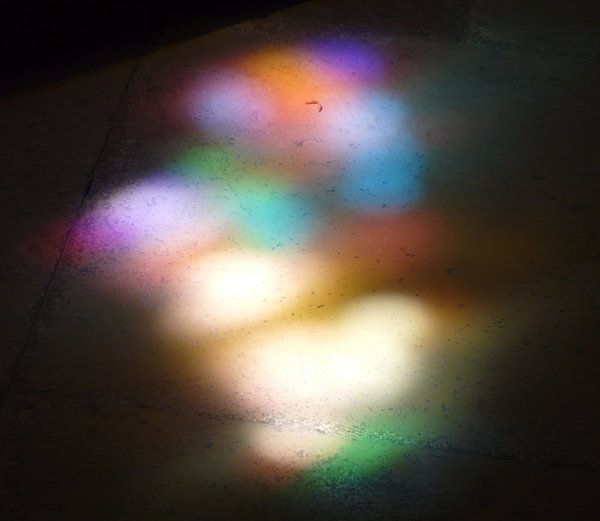
\includegraphics[height=6cm]{lichtspiel.jpg}}
\end{dispListing}
{\tcbset{reset}\tcbusetemp}

\end{docTcbKey}



\clearpage
\subsection{Embedding into the Surroundings}\label{subsec:surroundings}
Typically, but not necessarily, a |tcolorbox| is put inside a separate paragraph
and has some vertical space before and after it.
This behavior is controlled by the keys |before| and |after|.

\begin{docTcbKey}{before}{=\meta{code}}{no default, initially see \refKey{/tcb/autoparskip}}
  Sets the \meta{code} which is executed before the colored box.
  It is not used for floating boxes.
  Also, it is not used, if the box follows a heading immediately
  and \refKey{/tcb/ignore nobreak} is set to \docValue{false}.
\end{docTcbKey}

\begin{docTcbKey}{after}{=\meta{code}}{no default, initially see \refKey{/tcb/autoparskip}}
  Sets the \meta{code} which is executed after the colored box.
  It is not used for floating boxes.
\end{docTcbKey}

\begin{docTcbKey}{parskip}{}{style, no value}
  Sets the keys |before| and |after| to values which are
  recommended, if the package |parskip| \emph{is} used and there is no better
  idea for |before| and |after|. This is similar to:
\begin{dispListing}
\tcbset{parskip/.style={before={\par\pagebreak[0]\parindent=0pt},
                        after={\par}}}
\end{dispListing}
\end{docTcbKey}

\begin{docTcbKey}[][doc updated=2016-02-14]{noparskip}{}{style, no value}
  Sets the keys |before| and |after| to values which are
  recommended, if the package |parskip| is \emph{not} used and there is no better
  idea for |before| and |after|. This is similar to:
\begin{dispListing}
\tcbset{noparskip/.style={before={\par\pagebreak[0]\smallskip\parindent=0pt},
                          after={\par\smallskip}}}
\end{dispListing}
\end{docTcbKey}

\begin{docTcbKey}{autoparskip}{}{style, no value, initially set}
  Tries to detect the usage of the package |parskip| and sets
  the keys |before| and |after| accordingly. Actually, the following is done:
  \begin{itemize}
  \item If the length of |\parskip| is greater than |0pt| at the beginning of the document,
    \refKey{/tcb/parskip} is executed. Here, the usage of package |parskip| is \emph{assumed}.
  \item Otherwise, if the length of |\parskip| is not greater than |0pt| at the beginning of the document,
    \refKey{/tcb/noparskip} is executed. Here, the absence of package |parskip| is \emph{assumed}.
  \end{itemize}
  |autoparskip| is the default for the package |tcolorbox|, if |before| or |after|
  are not changed otherwise.
\end{docTcbKey}

\begin{docTcbKey}{nobeforeafter}{}{style, no value}
  Abbreviation for clearing the keys |before| and |after|. The colored box
  is not put into a paragraph and there is no space before or after the box.
\begin{dispExample}
\tcbset{myone/.style={colback=LightGreen,colframe=DarkGreen,
  equal height group=nobefaf,width=\linewidth/4,nobeforeafter}}
\begin{tcolorbox}[myone,title=Box 1]Box 1\end{tcolorbox}%
\begin{tcolorbox}[myone,title=Box 2]Box 2\end{tcolorbox}%
\begin{tcolorbox}[myone,title=Box 3]Box 3\end{tcolorbox}%
\begin{tcolorbox}[myone,title=Box 4]Box 4\end{tcolorbox}
\end{dispExample}
\end{docTcbKey}

\enlargethispage*{1cm}
\begin{docTcbKey}{forces nobeforeafter}{}{style, no value}
  Forces the setting of \refKey{/tcb/nobeforeafter} even if
  \refKey{/tcb/before} and \refKey{/tcb/after} are set to other values
  later. Do not use this option globally unless you \emph{really} know what you do.
  Note that embedded boxes do not inherit this forced clearance.
\end{docTcbKey}


\clearpage

\begin{docTcbKey}{baseline}{=\meta{length}}{no default, initially |0pt|}
  Used to set the |\pgfsetbaseline| value of the resulting |tcolorbox|.
\begin{dispExample}
\tcbset{colframe=red!50!white,width=4cm,nobeforeafter}
Some text\dotfill
\begin{tcolorbox}[baseline=3mm]
One line.
\end{tcolorbox}
\begin{tcolorbox}[baseline=3mm]
First line.\\Second line.
\end{tcolorbox}
\end{dispExample}
\end{docTcbKey}


\begin{docTcbKey}[][doc new=2014-10-10]{box align}{=\meta{alignment}}{style, no default, initially |bottom|}
  Used to set the \refKey{/tcb/baseline} value of the resulting |tcolorbox|.
  Feasible values for \meta{alignment} are:
  \begin{itemize}
  \item\docValue{bottom}: alignment with the box bottom,
  \item\docValue{top}: alignment with the box top,
  \item\docValue{center}: alignment with the box center,
  \item\docValue{base}: alignment with the box content base. This option
    is not applicable for a \refEnv{tcolorbox} but for a \refCom{tcbox} only.
    It is an alias for \refKey{/tcb/tcbox raise base}.
  \end{itemize}

\begin{dispExample}
\tcbset{colframe=red!50!white,width=4cm,nobeforeafter}
Some text\dotfill
\begin{tcolorbox}[box align=bottom]
One line.
\end{tcolorbox}
\begin{tcolorbox}[box align=bottom]
First line.\\Second line.
\end{tcolorbox}
\end{dispExample}

\begin{dispExample}
\tcbset{colframe=red!50!white,width=4cm,nobeforeafter}
Some text\dotfill
\begin{tcolorbox}[box align=top]
One line.
\end{tcolorbox}
\begin{tcolorbox}[box align=top]
First line.\\Second line.
\end{tcolorbox}
\end{dispExample}

\begin{dispExample}
\tcbset{colframe=red!50!white,width=4cm,nobeforeafter}
Some text\dotfill
\begin{tcolorbox}[box align=center]
One line.
\end{tcolorbox}
\begin{tcolorbox}[box align=center]
First line.\\Second line.
\end{tcolorbox}
\end{dispExample}

\begin{dispExample}
\tcbset{colframe=red!50!white,nobeforeafter}
Some text\dotfill
\tcbox[nobeforeafter,box align=base]{One line}
\tcbox[nobeforeafter,box align=base,size=fbox]{Another line}
\end{dispExample}
\end{docTcbKey}


\begin{docTcbKey}[][doc new and updated={2014-10-10}{2015-03-16}]{before skip}{=\meta{glue}}{style, no default}
  Inserts some vertical space of the given \meta{glue} before the colored box.
  This style sets \refKey{/tcb/before}.
\begin{dispExample*}{sbs,lefthand ratio=0.6}
Some text.
\begin{tcolorbox}[before skip=1cm,
    colframe=red!50!white]
  This is a \textbf{tcolorbox}.
\end{tcolorbox}
\end{dispExample*}
\end{docTcbKey}

\begin{docTcbKey}[][doc new and updated={2014-10-10}{2015-03-16}]{after skip}{=\meta{glue}}{style, no default}
  Inserts some vertical space of the given \meta{glue} after the colored box.
  This style sets \refKey{/tcb/after}.
\begin{dispExample*}{sbs,lefthand ratio=0.6}
\begin{tcolorbox}[after skip=1cm,
    colframe=red!50!white]
  This is a \textbf{tcolorbox}.
\end{tcolorbox}
Some text.
\end{dispExample*}
\end{docTcbKey}

\begin{docTcbKey}[][doc new=2014-10-10]{beforeafter skip}{=\meta{glue}}{style, no default}
  Inserts some vertical space of the given \meta{glue} before \emph{and} after the colored box.
  This style sets \refKey{/tcb/before} and \refKey{/tcb/after}.
\begin{dispExample*}{sbs,lefthand ratio=0.6}
\tcbset{beforeafter skip=0pt,
  colframe=red!50!white}
\begin{tcolorbox}
  This is a \textbf{tcolorbox}.
\end{tcolorbox}
\begin{tcolorbox}
  Second box.
\end{tcolorbox}
\end{dispExample*}
\end{docTcbKey}

\clearpage

\begin{docTcbKey}[][doc new=2014-11-07]{left skip}{=\meta{length}}{style, no default, initially |0mm|}
  Inserts some horizontal space of the given \meta{length} before the colored box.
  This style sets \refKey{/tcb/grow to left by} with the negated \meta{length},
  i.e. the bounding box and box width are changed.
\begin{dispExample*}{sbs,lefthand ratio=0.6}
\noindent\rule{\linewidth}{2pt}

\begin{tcolorbox}[left skip=1cm,
    colframe=red!50!white]
  This is a \textbf{tcolorbox}.
\end{tcolorbox}
\end{dispExample*}
\end{docTcbKey}

\begin{docTcbKey}[][doc new=2014-11-07]{right skip}{=\meta{length}}{style, no default, initially |0mm|}
  Inserts some horizontal space of the given \meta{length} after the colored box.
  This style sets \refKey{/tcb/grow to right by} with the negated \meta{length},
  i.e. the bounding box and box width are changed.
\begin{dispExample*}{sbs,lefthand ratio=0.6}
\noindent\rule{\linewidth}{2pt}

\begin{tcolorbox}[right skip=1cm,
    colframe=red!50!white]
  This is a \textbf{tcolorbox}.
\end{tcolorbox}
\end{dispExample*}
\end{docTcbKey}

\begin{docTcbKey}[][doc new=2014-10-10]{leftright skip}{=\meta{length}}{style, no default}
  Inserts some horizontal space of the given \meta{length} before \emph{and} after the colored box.
  This style changes the bounding box and the box width.
\begin{dispExample*}{sbs,lefthand ratio=0.6}
\noindent\rule{\linewidth}{2pt}

\begin{tcolorbox}[leftright skip=1cm,
    colframe=red!50!white]
  This is a \textbf{tcolorbox}.
\end{tcolorbox}
\end{dispExample*}
\end{docTcbKey}


\begin{docTcbKey}[][doc new=2014-12-11]{ignore nobreak}{\colOpt{=true\textbar false}}{default |true|, initially |false|}
After a heading, \LaTeX\ tries to avoid a break by setting a |nobreak| boolean value.
Starting from version |3.33|, the \refKey{/tcb/before} respectively \refKey{/tcb/before skip}
settings are not used after a heading if \refKey{/tcb/ignore nobreak} is
set to \docValue{false}. For an unbreakable box, \refKey{/tcb/before nobreak} is used instead.
Further, a \refKey{/tcb/breakable} box will also try to
avoid a break between a heading and a directly following first part of a
break sequence.

Set \refKey{/tcb/ignore nobreak} to \docValue{true}, if |nobreak| should be
ignored as prior to version |3.33|. Also, such a setting may be used locally to
enforce the \refKey{/tcb/before} setting.
\end{docTcbKey}

\begin{docTcbKey}[][doc new=2014-12-16]{before nobreak}{=\meta{code}}{no default, initially \cs{noindent}}
  Sets the \meta{code} which is executed before the colored box if it
  is unbreakable, if \refKey{/tcb/ignore nobreak} is not set, and if
  the box follows a heading.
\end{docTcbKey}


\clearpage
\subsection{Bounding Box}
Normally, every |tcolorbox| has a bounding box which fits exactly to the
dimensions of the outer frame. Therefore, \LaTeX\ reserves exactly the space
needed for the box.
This behavior can be changed by enlarging (or shrinking) the bounding box.
If the bounding box is enlarged, the |tcolorbox| will get some clearance
around it. If the bounding box is shrunk, i.\,e.\ enlarged with negative
values, the |tcolorbox| will overlap to other parts of the page.
For example, the |tcolorbox| could be stretched into the page margin.

\begin{marker}
The following examples use \refKey{/tcb/show bounding box} to display the
actual bounding box. For this, the library \mylib{skins} has to be included and
\refKey{/tcb/enhanced} has to be set.
\end{marker}

\begin{docTcbKey}{enlarge top initially by}{=\meta{length}}{no default, initially |0mm|}
  Enlarges the bounding box distance to the top of the box by \meta{length}.
  If the box is \emph{breakable}, only the first box of the break sequence
  gets enlarged. \refKey{/tcb/enlarge top by} overwrites this key.
\begin{dispExample}
\tcbset{colframe=blue!75!black,colback=white}

\begin{tcolorbox}[enlarge top initially by=-5mm]
This is a \textbf{tcolorbox}.
\end{tcolorbox}
\begin{tcolorbox}[enlarge top initially by=5mm,enhanced,show bounding box]
This is a \textbf{tcolorbox}.
\end{tcolorbox}
\end{dispExample}
\end{docTcbKey}



\begin{docTcbKey}{enlarge bottom finally by}{=\meta{length}}{no default, initially |0mm|}
  Enlarges the bounding box distance to the bottom of the box by \meta{length}.
  If the box is \emph{breakable}, only the last box of the break sequence
  gets enlarged. \refKey{/tcb/enlarge bottom by} overwrites this key.
\begin{dispExample}
\tcbset{colframe=blue!75!black,colback=white}

\begin{tcolorbox}[enlarge bottom finally by=5mm]
This is a \textbf{tcolorbox}.
\end{tcolorbox}
\begin{tcolorbox}[enlarge bottom finally by=-5mm,enhanced,show bounding box]
This is a \textbf{tcolorbox}.
\end{tcolorbox}
\end{dispExample}
\end{docTcbKey}

\clearpage


\begin{docTcbKey}{enlarge top at break by}{=\meta{length}}{no default, initially \texttt{0mm}}
  Enlarges the bounding box distance to the top of the box by \meta{length},
  \emph{if} the box is \refKey{/tcb/breakable}.
  In this case, it is applied to \emph{middle} and \emph{last} parts in a
  break sequence.
  \refKey{/tcb/enlarge top by} overwrites this key.
\end{docTcbKey}


\begin{docTcbKey}{enlarge bottom at break by}{=\meta{length}}{no default, initially \texttt{0mm}}
  Enlarges the bounding box distance to the bottom of the box by \meta{length},
  \emph{if} the box is \refKey{/tcb/breakable}.
  In this case, it is applied to \emph{first} and \emph{middle} parts in a
  break sequence. \refKey{/tcb/enlarge bottom by} overwrites this key.
\end{docTcbKey}


\begin{docTcbKey}{enlarge top by}{=\meta{length}}{no default, initially |0mm|}
  Enlarges the bounding box distance to the top of the box by \meta{length}.
  \refKey{/tcb/enlarge top initially by} and
  \refKey{/tcb/enlarge top at break by} are set to \meta{length}.
\end{docTcbKey}


\begin{docTcbKey}{enlarge bottom by}{=\meta{length}}{no default, initially |0mm|}
  Enlarges the bounding box distance to the bottom of the box by \meta{length}.
  \refKey{/tcb/enlarge bottom finally by} and
  \refKey{/tcb/enlarge bottom at break by} are set to \meta{length}.
\end{docTcbKey}


\begin{docTcbKey}{enlarge left by}{=\meta{length}}{no default, initially |0mm|}
  Enlarges the bounding box distance to the left side of the box by \meta{length}.
\begin{dispExample}
\tcbset{colframe=blue!75!black,colback=white}

\begin{tcolorbox}[enlarge left by=2cm,width=5cm,enhanced,show bounding box]
This is a \textbf{tcolorbox}.
\end{tcolorbox}
\begin{tcolorbox}[enlarge left by=-2cm,width=\linewidth+2cm]
This is a \textbf{tcolorbox}.
\end{tcolorbox}
\end{dispExample}
\end{docTcbKey}

\begin{docTcbKey}{enlarge right by}{=\meta{length}}{no default, initially |0mm|}
  Enlarges the bounding box distance to the right side of the box by \meta{length}.
\begin{dispExample}
\tcbset{colframe=blue!75!black,colback=white}

\begin{tcolorbox}[enlarge right by=-2cm,width=\linewidth+2cm,
  enhanced,show bounding box]
This is a \textbf{tcolorbox}.
\end{tcolorbox}
\begin{tcolorbox}[enlarge right by=2cm,width=\linewidth-2cm]
This is a \textbf{tcolorbox}.
\end{tcolorbox}
\end{dispExample}
\end{docTcbKey}

\clearpage
\begin{docTcbKey}{enlarge by}{=\meta{length}}{no default, initially |0mm|}
  Enlarges the bounding box distance to all sides of the box by \meta{length}.
\begin{dispExample}
\tcbset{colframe=blue!75!black,colback=white,width=5cm,nobeforeafter}

\begin{tcolorbox}
This is a \textbf{tcolorbox}.
\end{tcolorbox}
\begin{tcolorbox}[enlarge by=5mm,enhanced,show bounding box]
This is a \textbf{tcolorbox}.
\end{tcolorbox}
\end{dispExample}
\end{docTcbKey}



\begin{docTcbKey}[][doc new=2015-11-20]{flush left}{}{style, no value}
  Enlarges the bounding box to the right side to fill the line completely.
\begin{dispExample}
\tcbset{colframe=blue!75!black,colback=white}

\begin{tcolorbox}[flush left,width=5cm,enhanced,show bounding box]
This is a \textbf{tcolorbox}.
\end{tcolorbox}
\end{dispExample}
\end{docTcbKey}


\begin{docTcbKey}[][doc new=2015-11-20]{flush right}{}{style, no value}
  Enlarges the bounding box to the left side to fill the line completely.
\begin{dispExample}
\tcbset{colframe=blue!75!black,colback=white}

\begin{tcolorbox}[flush right,width=5cm,enhanced,show bounding box]
This is a \textbf{tcolorbox}.
\end{tcolorbox}
\end{dispExample}
\end{docTcbKey}


\begin{docTcbKey}[][doc new=2015-11-20]{center}{}{style, no value}
  Enlarges the bounding box equally to both sides to fill the line completely.
\begin{dispExample}
\tcbset{colframe=blue!75!black,colback=white}

\begin{tcolorbox}[center,width=5cm,enhanced,show bounding box]
This is a \textbf{tcolorbox}.
\end{tcolorbox}
\end{dispExample}
\end{docTcbKey}

\clearpage
\begin{docTcbKey}{grow to left by}{=\meta{length}}{no default, initially |0mm|}
  Enlarges the current box width by \meta{length} and
  enlarges (shrinks) the bounding box distance to the left side of the box by
  $-$\meta{length}. Also see \refKey{/tcb/left skip}.
\begin{dispExample}
\tcbset{colframe=blue!75!black,colback=white}

\begin{tcolorbox}[width=5cm,grow to left by=2cm,enhanced,show bounding box]
This is a \textbf{tcolorbox} with a width of 7cm.
\end{tcolorbox}
\end{dispExample}
\end{docTcbKey}

\begin{docTcbKey}{grow to right by}{=\meta{length}}{no default, initially |0mm|}
  Enlarges the current box width by \meta{length} and
  enlarges (shrinks) the bounding box distance to the right side of the box by
  $-$\meta{length}. Also see \refKey{/tcb/right skip}.
\begin{dispExample}
\tcbset{colframe=blue!75!black,colback=white}

\begin{tcolorbox}[grow to right by=2cm,enhanced,show bounding box]
This is a \textbf{tcolorbox}.
\end{tcolorbox}

\bigskip

\begin{tcolorbox}[grow to right by=2cm,grow to left by=1cm,
  enhanced,show bounding box]
This is a \textbf{tcolorbox}.
\end{tcolorbox}

\end{dispExample}
\end{docTcbKey}


\clearpage
\begin{docTcbKey}[][doc updated=2015-11-13]{toggle enlargement}{=\meta{toggle preset}}{default |evenpage|, initially |none|}
  According to the \meta{toggle preset}, the left and the right enlargements of
  the bounding box are switched or not. Feasible values are:
  \begin{itemize}
  \item\docValue{none}: no switching.
  \item\docValue{forced}: the values of the left and right enlargement are switched.
  \item\docValue{evenpage}: if the page is an even page, the values of the left and
    right enlargement are switched. This value also sets
    \refKey{/tcb/check odd page} to |true|.
    %It is recommended that you use this setting in
    %conjunction with \refKey{/tcb/check odd page}.
    %Note that the page number detection may
    %fail in certain cases. For these cases, use the |forced| value.
  \end{itemize}
\begin{marker}
See \refKey{/tcb/toggle left and right} to toggle geometry settings.
\end{marker}

\begin{dispExample}
\tcbset{colframe=blue!75!black,colback=white,
  grow to left by=20mm,grow to right by=-5mm}

\begin{tcolorbox}[toggle enlargement=none,enhanced,show bounding box]
This is a \textbf{tcolorbox}.
\end{tcolorbox}
\begin{tcolorbox}[toggle enlargement=forced]
This is a \textbf{tcolorbox}.
\end{tcolorbox}
\begin{tcolorbox}[toggle enlargement=evenpage]
  This page is an \tcbifoddpage{odd}{even} page.
  Therefore, the left and right enlargements
  \tcbifoddpage{are not}{are} toggled.
\end{tcolorbox}
\end{dispExample}

\begin{dispListing}
\begin{tcolorbox}[colframe=red!60!black,colback=red!15!white,
  fonttitle=\bfseries,title=Floating box from \texttt{toggle enlargement},
  width=\textwidth,grow to right by=2cm,toggle enlargement,float=t]
  This page is an \tcbifoddpage{odd}{even} page.
  Therefore, the left and right enlargements \tcbifoddpage{are not}{are} toggled.
  This box stretches to the right margin on odd pages and to the left
  margin on even pages. The current document is one-sided -- this feature makes
  sense for two-sided documents only.
\end{tcolorbox}
\end{dispListing}
\tcbusetemp
\end{docTcbKey}


\clearpage
\begin{marker}
The following keys should not be used with breakable boxes or boxes with a
lower part.
\end{marker}

\begin{docTcbKey}{shrink tight}{}{style, no value, initially unset}
  The total colored box is shrunk to the dimensions of the upper
  part. There should be no lower part and no title.
  This style sets the \refKey{/tcb/boxsep} to |0pt| and other geometry keys
  to fitting values. This option is likely to be used with the following
  extrusion keys.
\begin{dispExample}
\tcbset{colframe=blue!75!black,colback=white,arc=0mm,boxrule=0.4pt,
        nobeforeafter,tcbox raise base,shrink tight}

\begin{tcolorbox}
This is a \textbf{tcolorbox}.
\end{tcolorbox}

Lorem \tcbox{ipsum} dolor sit amet, consectetuer adipiscing elit.
\end{dispExample}
\end{docTcbKey}

\begin{docTcbKey}[][doc updated=2014-09-19]{extrude left by}{=\meta{length}}{style, no default, initially unset}
  The (upper part of the) colored box is extruded by the given \meta{length} to the left side.
  The inner width and the bounding box is kept unchanged and the operation
  is additive!
\begin{dispExample}
\tcbset{enhanced,colframe=red,colback=yellow!25!white,
  frame style={opacity=0.25},interior style={opacity=0.5},
  nobeforeafter,tcbox raise base,shrink tight,extrude by=2mm}

Lorem ipsum dolor sit amet, consectetuer adipiscing elit. Ut purus elit,
vestibulum ut, placerat ac, adipiscing vitae, felis.
\tcbox[extrude left by=1cm]{Curabitur} dictum gravida mauris.
Nam arcu libero, nonummy eget, consectetuer id, vulputate a, magna.
\end{dispExample}
\end{docTcbKey}

\begin{docTcbKey}[][doc updated=2014-09-19]{extrude right by}{=\meta{length}}{style, no default, initially unset}
  The (upper part of the) colored box is extruded by the given \meta{length} to the right side.
  The inner width and the bounding box is kept unchanged and the operation
  is additive!
\begin{dispExample}
\tcbset{enhanced,colframe=red,colback=yellow!25!white,
  frame style={opacity=0.25},interior style={opacity=0.5},
  nobeforeafter,tcbox raise base,shrink tight,extrude by=2mm}

Lorem ipsum dolor sit amet, consectetuer adipiscing elit. Ut purus elit,
vestibulum ut, placerat ac, adipiscing vitae, felis.
\tcbox[extrude right by=1cm]{Curabitur} dictum gravida mauris.
Nam arcu libero, nonummy eget, consectetuer id, vulputate a, magna.
\end{dispExample}
\end{docTcbKey}

\clearpage
\begin{docTcbKey}{extrude top by}{=\meta{length}}{style, no default, initially unset}
  The (upper part of the) colored box is extruded by the given \meta{length} to the top side.
  The inner width and the bounding box is kept unchanged and the operation
  is additive!
\begin{dispExample}
\tcbset{enhanced,colframe=red,colback=yellow!25!white,
  frame style={opacity=0.25},interior style={opacity=0.5},
  nobeforeafter,tcbox raise base,shrink tight,extrude by=2mm}

Lorem ipsum dolor sit amet, consectetuer adipiscing elit. Ut purus elit,
vestibulum ut, placerat ac, adipiscing vitae, felis.
\tcbox[extrude top by=1cm]{Curabitur} dictum gravida mauris.
Nam arcu libero, nonummy eget, consectetuer id, vulputate a, magna.
\end{dispExample}
\end{docTcbKey}

\begin{docTcbKey}{extrude bottom by}{=\meta{length}}{style, no default, initially unset}
  The (upper part of the) colored box is extruded by the given \meta{length} to the bottom side.
  The inner width and the bounding box is kept unchanged and the operation
  is additive!
\begin{dispExample}
\tcbset{enhanced,colframe=red,colback=yellow!25!white,
  frame style={opacity=0.25},interior style={opacity=0.5},
  nobeforeafter,tcbox raise base,shrink tight,extrude by=2mm}

Lorem ipsum dolor sit amet, consectetuer adipiscing elit. Ut purus elit,
vestibulum ut, placerat ac, adipiscing vitae, felis.
\tcbox[extrude bottom by=1cm]{Curabitur} dictum gravida mauris.
Nam arcu libero, nonummy eget, consectetuer id, vulputate a, magna.
\end{dispExample}
\end{docTcbKey}

\begin{docTcbKey}{extrude by}{=\meta{length}}{style, no default, initially unset}
  The (upper part of the) colored box is extruded by the given \meta{length} to all sides.
  The inner width and the bounding box is kept unchanged and the operation
  is additive!
\begin{dispExample}
\tcbset{enhanced,colframe=red,colback=yellow!25!white,
  frame style={opacity=0.25},interior style={opacity=0.5},
  nobeforeafter,tcbox raise base,shrink tight,extrude by=2mm}

Lorem ipsum dolor sit amet, consectetuer adipiscing elit. Ut purus elit,
vestibulum ut, placerat ac, adipiscing vitae, felis. \tcbox{Curabitur} dictum
gravida mauris. \tcbox[colframe=Green,interior style={opacity=0.0}]{Nam}
arcu libero, nonummy eget, consectetuer id, \tcbox{vulputate} a, magna. Donec
vehicula augue eu neque. Pellentesque habitant morbi tristique senectus et netus
et malesuada fames ac turpis egestas. \tcbox{Mauris ut leo.}
\end{dispExample}
\end{docTcbKey}

\clearpage
\subsection{Layered Boxes and Every Box Settings}\label{subsec:everybox}
A |tcolorbox| may contain another |tcolorbox| and so on. The package
takes track of the nesting level using a counter |tcblayer|. Counter values
may be used for doing some fancy things, but you should never change
the counter value yourself.

The package takes special care for the first four layers or nesting levels,
called managed layers.
Here, footnote texts are administrated to find their intended place
and specific layer dependent options may be set by changing
\refKey{/tcb/every box on layer n}.
If needed, the number of managed layers can be increased by setting
\refCom{tcbsetmanagedlayer} to a higher value than~4.

The following styles have a considerable influence on how layered boxes
are processed. Note especially that nested boxes are getting a
\refKey{/tcb/reset} by default. You can change this, but be prepared for
suprises if you do.

If the defaults are \emph{not changed}, a |tcolorbox| gets its options
in the following order. Following options overwrite preceding options.
\begin{enumerate}
\item On package load, all options are set to default values.
\item Every \refCom{tcbset} command adds or changes options for the following boxes
  inside the current \TeX\ group.
\item While entering a |tcolorbox|, a \refKey{/tcb/every box on layer n} or
  \refKey{/tcb/every box on higher layers} option list is applied.
  With default settings this means:
  \begin{itemize}
  \item For layer 1 (lowest layer), the \refKey{/tcb/every box} option list is applied.
    Not overwritten options given by a preceding \refCom{tcbset} survive.
  \item For layer 2 and above (nested boxes), a \refKey{/tcb/reset} followed by
    \refKey{/tcb/every box} option list is applied.
    Every resettable options given by a preceding \refCom{tcbset}
    and by the sourrounding box(es) are reset.
  \end{itemize}
\item The \meta{options} given to the |tcolorbox| are applied.
  Or, if the box was generated by \refCom{newtcolorbox} or friends,
  the \meta{options} given there are applied.
\item If the box was generated by \refCom{newtcolorbox} or friends,
  some automated options are applied.
\end{enumerate}


\begin{docTcbKey}{every box}{}{style}
By default, this style is empty.
\begin{dispListing}
% default setting:
\tcbset{every box/.style={}}
\end{dispListing}
It may be changed by redefining this style.
\begin{dispListing}
% setting all boxes to be enhanced:
\tcbset{every box/.style={enhanced}}
\end{dispListing}

\medskip
\begin{marker}
The alternative for setting something for every box (on every layer) is\\
\refCom{tcbsetforeverylayer}:
\begin{dispListing}
% setting all boxes to be enhanced:
\tcbsetforeverylayer{enhanced}
\end{dispListing}
\end{marker}
\end{docTcbKey}

\clearpage
\begin{docTcbKey}{every box on layer n}{}{style}
Here, |n| has to be replaced by a number ranging from 1 to the highest
managed layer number (4 by default).
\begin{dispListing}
% default settings:
\tcbset{
  every box on layer 1/.style={every box},
  every box on layer 2/.style={reset,every box},
  every box on layer 3/.style={reset,every box},
  every box on layer 4/.style={reset,every box},
  }
\end{dispListing}
\end{docTcbKey}


\begin{docTcbKey}{every box on higher layers}{}{style}
Higher layers are layers above the highest
managed layer number (4 by default).
\begin{dispListing}
\tcbset{every box on higher layers/.style={reset,every box}}
\end{dispListing}
\end{docTcbKey}


\begin{docCommand}{tcbsetmanagedlayer}{\marg{number}}
Replaces the highest managed layer number by \meta{number} where 4 is
the default. This macro can only be used inside the preamble.
Using a \meta{number} lower than 4 typically makes no sense, but is
not forbidden.
\end{docCommand}

\begin{tcboutputlisting}
% \usepackage{lipsum}
% \tcbuselibrary{skins,breakable}
\tcbset{colframe=red!75!black,fonttitle=\bfseries,
  colback=red!5!white,
  every box/.style={enhanced,watermark text=\thetcblayer,
    before=\par\smallskip,after=\par\smallskip},
  every box on layer 2/.style={reset,every box,colback=yellow!10!white,
    drop fuzzy shadow}}
\begin{tcolorbox}[enhanced jigsaw,breakable,title=Layer 1 Box]
Here comes a footnote\footnote{Footnote from layer 1 box}.
\lipsum[2]
  \begin{tcolorbox}[title=Layer 2 Box]
  abc\footnote{The footnote of abc}
  \end{tcolorbox}
  \begin{tcolorbox}[title=Another Box,ams equation]
    \tcbhighmath{\sum\limits_{n=1}^{\infty} \frac{1}{n}} = \infty.
  \end{tcolorbox}
Some text\footnote{Footnote from some text}.
  \begin{tcolorbox}[title=Yet Another Box]
    \tcboxfit[height=2cm]{\lipsum[1]}
    My text.
    \begin{tcolorbox}
      Another lipsum text\footnote{A lipsum text}. \lipsum[3]
      \begin{tcolorbox}[title=Layer 4,colframe=blue,colback=white]
        Layer 4\footnote{Layer 4 footnote}
      \end{tcolorbox}
      The End\footnote{Last footnote}.
    \end{tcolorbox}
  \end{tcolorbox}
\end{tcolorbox}
\end{tcboutputlisting}

\tcbinputlisting{base example,listing only,listing style=mydocumentation}

{\tcbuselistingtext}


\clearpage
\subsection{Capture Mode}\label{subsec:capture}

\begin{docTcbKey}{capture}{=\meta{mode}}{no default, initially |minipage|}
  The capture \meta{mode} defines how the box content is processed.

Feasible values for \meta{mode} are:
\begin{itemize}
\item\docValue{minipage}:\\
  This is the default \meta{mode} for \refEnv{tcolorbox}.
  The content may have an upper and a lower part. Optionally, the box
  can be \refKey{/tcb/breakable}. The box content is put into a
  minipage or into something similar to a minipage.
\item\docValue{hbox}:\\
  This is the default \meta{mode} for \refCom{tcbox}. The content cannot have
  a lower part and cannot be broken. The colored box is sized according
  to the dimensions of the content.
  A shortcut to set this mode is \refKey{/tcb/hbox}.
\item\docValue{fitbox}: (needs the \mylib{fitting} library)\\
  This is the default \meta{mode} for \refCom{tcboxfit}. The content cannot have
  a lower part and cannot be broken.
  The content is sized according to the dimensions of the colored box.
  A shortcut to set this mode is \refKey{/tcb/fit}.
\end{itemize}

\begin{dispExample}
\tcbset{colframe=blue!75!black,colback=white}

\begin{tcolorbox}[capture=minipage]
This is a tcolorbox.
\end{tcolorbox}

\begin{tcolorbox}[capture=hbox]
This is a tcolorbox.
\end{tcolorbox}

\begin{tcolorbox}[capture=fitbox,height=9mm]% needs the 'fitting' library
This is a tcolorbox.
\end{tcolorbox}
\end{dispExample}
\end{docTcbKey}



\begin{docTcbKey}{hbox}{}{style, no default}
  Shortcut for |capture=hbox|.
\begin{dispExample}
\tcbset{colframe=blue!75!black,colback=white}

\begin{tcolorbox}[hbox]
This is a tcolorbox.
\end{tcolorbox}
\end{dispExample}
\end{docTcbKey}


\begin{docTcbKey}{minipage}{}{style, no default}
  Shortcut for |capture=minipage|.
\end{docTcbKey}


\clearpage
\subsection{Text Characteristics}
\begin{docTcbKey}[][doc updated=2015-10-14]{parbox}{\colOpt{=true\textbar false}}{default |true|, initially |true|}
  The text inside a |tcolorbox| is formatted using a \LaTeX\ |minipage|
  if the box is unbreakable. If breakable, the box tries a mimicry of
  a |minipage|. In a |minipage| or |parbox|, paragraphs are formatted slightly different
  as the main text. If the key value is set to |false|, the normal main text
  behavior is restored. In some situations, this has some unwanted side
  effects. It is recommended that you use this experimental setting only
  where you really want to have this feature.
\end{docTcbKey}

\begin{dispListing}
% \usepackage{lipsum}  % preamble
\tcbset{width=(\linewidth-2mm)/2,nobeforeafter,arc=1mm,
  colframe=blue!75!black,colback=white,fonttitle=\bfseries,fontupper=\small,
  left=2mm,right=2mm,top=1mm,bottom=1mm,equal height group=parbox}

\begin{tcolorbox}[parbox,adjusted title={parbox=true (normal)}]
  \lipsum[1-2]
\end{tcolorbox}\hfill%
\begin{tcolorbox}[parbox=false,adjusted title={parbox=false}]
  \lipsum[1-2]
\end{tcolorbox}%
\end{dispListing}
{\tcbusetemp}


\clearpage
\begin{docTcbKey}{hyphenationfix}{\colOpt{=true\textbar false}}{default |true|, initially |false|}
  Long words at the beginning of paragraphs in very narrow boxes
  will not be hyphenated using |pdflatex|. This problem is circumvented by
  applying the |hyphenationfix| option.

\begin{dispExample*}{sbs,lefthand ratio=0.6}
\tcbset{colframe=blue!75!black,
  fontupper=\normalsize,
  colback=blue!5!white,width=4cm}

\begin{tcolorbox}
Rechnungsadjunktentochter.\par
Statthaltereikonzipist.
\end{tcolorbox}

\begin{tcolorbox}[hyphenationfix]
Rechnungsadjunktentochter.\par
Statthaltereikonzipist.
\end{tcolorbox}
\end{dispExample*}

\smallskip
\begin{marker}
|parbox=false| and |hyphenationfix| should not be used together. They are
targeting different box types and they do not blend very well.
\end{marker}
\end{docTcbKey}


\subsection{Files}
\begin{docTcbKey}{tempfile}{=\meta{file name}}{no default, initially \cs{jobname.tcbtemp}}
  Sets \meta{file name} as name for the temporary file which is used inside
  \refEnv{tcbwritetemp} and \refCom{tcbusetemp} implicitely.
\end{docTcbKey}

\subsection{\texttt{\textbackslash tcbox} Specials}
The following options are applicable for \refCom{tcbox} and \refCom{tcboxmath}
only.

\begin{docTcbKey}{tcbox raise}{=\meta{length}}{no default, initially \texttt{0pt}}
  Raises the \refCom{tcbox} by the given \meta{length}.
 % Sets the line width of the right rule to \meta{length}.
\begin{dispExample}
\tcbset{colframe=blue!50!black,colback=white,colupper=red!50!black,
        fonttitle=\bfseries,nobeforeafter,center title}

Test\dotfill
\tcbox[tcbox raise base]{Hello World 1}\dotfill
\tcbox{Hello World 2}\dotfill
\tcbox[tcbox raise=5mm]{Hello World 3}
\end{dispExample}
\end{docTcbKey}

\begin{docTcbKey}{tcbox raise base}{}{style, no value, initially unset}
  Raises the \refCom{tcbox} such that the base of its content matches
  the base of the environmental line; see example above.
\end{docTcbKey}

\begin{docTcbKey}{on line}{}{style, no value, initially unset}
  Combines \refKey{/tcb/tcbox raise base} with \refKey{/tcb/nobeforeafter}.
  The resulting box behaves analogue to |\fbox|.
\end{docTcbKey}

\clearpage
\begin{docTcbKey}[][doc new=2015-03-23]{tcbox width}{=\meta{mode}}{no default, initially \texttt{auto}}
Controls how \refCom{tcbox} respects a \refKey{/tcb/width} setting.
Feasible values for \meta{mode} are:
\begin{itemize}
\item\docValue{auto} (initial setting):
  ignore \refKey{/tcb/width} and set box width according to its content.
\item\docValue{auto limited}:
  Set box width according to its content, if it is smaller than \refKey{/tcb/width}.
  Otherwise, the content is set like in a \refEnv{tcolorbox} with line breaks.
\item\docValue{forced center}:
  Set box width according to \refKey{/tcb/width}.
  The content is centered and may overlap the box borders.
\item\docValue{forced left}:
  Set box width according to \refKey{/tcb/width}.
  The content is left aligned and may overlap the box borders.
\item\docValue{forced right}:
  Set box width according to \refKey{/tcb/width}.
  The content is right aligned and may overlap the box borders.
\item\docValue{minimum center}:
  Set box width according to \refKey{/tcb/width}, if the content fits into.
  The content is centered and the box width may grow beyond \refKey{/tcb/width}.
\item\docValue{minimum left}:
  Set box width according to \refKey{/tcb/width}, if the content fits into.
  The content is left aligned and the box width may grow beyond \refKey{/tcb/width}.
\item\docValue{minimum right}:
  Set box width according to \refKey{/tcb/width}, if the content fits into.
  The content is right aligned and the box width may grow beyond \refKey{/tcb/width}.
\end{itemize}

\enlargethispage*{1cm}

\begin{exdispExample}{tcbox_width}
\tcbset{size=small,on line,before upper=\strut,
  colframe=blue!75!black,colback=blue!5!white,
  fontupper=\normalsize,width=4cm}

\tcbox[tcbox width=auto]{auto}\qquad
\tcbox[tcbox width=auto limited]{auto limited}\qquad
\tcbox[tcbox width=auto limited]{auto limited with long text}\\
\tcbox[tcbox width=forced center]{forced center}\qquad
\tcbox[tcbox width=forced center]{forced center with long text}\\
\tcbox[tcbox width=forced left]{forced left}\qquad
\tcbox[tcbox width=forced left]{forced left with long text}\\
\tcbox[tcbox width=forced right]{forced right}\qquad
\tcbox[tcbox width=forced right]{forced right with long text}\\
\tcbox[tcbox width=minimum center]{minimum center}\qquad
\tcbox[tcbox width=minimum center]{minimum center with long text}\\
\tcbox[tcbox width=minimum left]{minimum left}\qquad
\tcbox[tcbox width=minimum left]{minimum left with long text}\\
\tcbox[tcbox width=minimum right]{minimum right}\qquad
\tcbox[tcbox width=minimum right]{minimum right with long text}
\end{exdispExample}
\end{docTcbKey}


%\subsection{Skins}
%There are additional option keys which change the appearance of a |tcolorbox|.
%If only the core package is used, there is only one \emph{skin} and these
%keys are meaningless.
%The library \mylib{skins} adds more skins. The appropriate option keys for skins of
%the core package are therefore described in \Vref{sec:skincorekeys} from
%page \pageref{sec:skincorekeys}.

\clearpage
\subsection{Counters, Labels, and References}

\begin{docTcbKey}{phantom}{=\meta{code}}{no default, initially unset}
The \meta{code} is put in a box at the upper left corner of the |tcolorbox|.
If the |tcolorbox| is breakable, the \meta{code} is executed for the first box of
the break sequence only. If there already was some phantom code given, the
new \meta{code} is appended.\par
The \meta{code} is intended to be used for counter stepping, labelling, and
related operations which do not produce visible text.
\begin{itemize}
\item The \meta{code} is executed before the title and box content, i.\,e.\ counter
  values are ensured to be increased before usage.
\item Labels are ensured to reference the correct page number.
\item The \meta{code} is executed only once even during fitting operations for
  title and box content.
\item In combination with the |hyperref| package, the hyper anchor is set
  to the upper left corner of the |tcolorbox|, i.\,e.\ links inside the pdf document
  will jump to the box pleasantly.
\item Since the \meta{code} is executed inside a \TeX\ group, only global
  operations can survive this group.
\end{itemize}
Examples for the |phantom| usage are given in Section \ref{listing:exercises}
from page \pageref{listing:exercises}, e.\,g.\
Example \ref{exe:tabular_example} on page \pageref{exe:tabular_example}.
\end{docTcbKey}

\begin{docTcbKey}{nophantom}{}{no value, initially set}
Removes the phantom code if set before.
\end{docTcbKey}

\begin{docTcbKey}{label}{=\meta{marker}}{no default, initially unset}
The \meta{marker} is set as label text for a reference with the |\ref| macro.
Typically, this option is used for numbered boxes, see Subsection \ref{sec:numberedboxes}
from page \pageref{sec:numberedboxes}, e.\,g.\ \refKey{/tcb/new/auto counter}.
\end{docTcbKey}

\begin{docTcbKey}[][doc new=2014-11-28]{phantomlabel}{=\meta{marker}}{no default, initially unset}
Equivalent to \refKey{/tcb/label} for an \emph{unnumbered} box.
A |\phantomsection| from the package |hyperref| is used to set a correct
hyperlink target. This is not needed for a numbered box.
\end{docTcbKey}

\begin{docTcbKey}{label type}{=\meta{type}}{no default, initially unset}
This option key can be used only in conjunction with the |cleveref| package
\cite{cubitt:2013a} which has to be loaded separately.
\meta{type} has to be a cross-reference type \emph{known} to |cleveref|
like |theorem|, |algorithm|, |result|, etc. References made with |cleveref|
will use this type. Note that using |label type| will result in compilation
errors, if |cleveref| is not loaded.
For an example, see \Vref{theo:meanvaluetheorem}.
\end{docTcbKey}

\begin{docTcbKey}{no label type}{}{no value, initially set}
Removes a \refKey{/tcb/label type}, if set before.
\end{docTcbKey}

\begin{docTcbKey}{step}{=\meta{counter}}{no default, initially unset}
Shortcut for |phantom={\refstepcounter{#1}}|. The given \meta{counter} is
increased and ready for labelling. This option is not needed when
using the convenient automated numbering introduced with version 2.40,
see Subsection \ref{sec:numberedboxes}
from page \pageref{sec:numberedboxes}.
\end{docTcbKey}

\begin{docTcbKey}{step and label}{=\marg{counter}\marg{marker}}{no default, initially unset}
Shortcut for using \refKey{/tcb/step} and \refKey{/tcb/label}. This option is not needed when
using the convenient automated numbering introduced with version 2.40,
see Subsection \ref{sec:numberedboxes}
from page \pageref{sec:numberedboxes}.
\end{docTcbKey}


\clearpage
\begin{docTcbKey}{list entry}{=\meta{text}}{no default, initially unset}
If the \flqq list of tcolorbox(es)\frqq\ feature described in Subsection
\ref{sec:listsof} from page \pageref{sec:listsof} is used, this key
describes the \meta{text} for an entry into the generated list, e.\,g.
\begin{dispListing}
list entry={\protect\numberline{\thetcbcounter}My beautiful Example}
\end{dispListing}
See Section \ref{listing:exercises} from page \pageref{listing:exercises}
for a complete example.
\end{docTcbKey}

\begin{docTcbKey}[][doc new=2014-09-19]{list text}{=\meta{text}}{style, no default}
This is a shortcut for setting \refKey{/tcb/list entry} to\\
|\protect\numberline{\thetcbcounter}|\meta{text}.
So, the following settings are identical:
\begin{dispListing}
list text={My beautiful Example},
list entry={\protect\numberline{\thetcbcounter}My beautiful Example}
\end{dispListing}
See Section \ref{listing:exercises} from page \pageref{listing:exercises}
for a complete example.
\end{docTcbKey}

\begin{docTcbKey}{add to list}{=\marg{list}\marg{type}}{no default, initially unset}
If the \flqq list of tcolorbox(es)\frqq\ feature described in Subsection
\ref{sec:listsof} from page \pageref{sec:listsof} is used, list entries are
generated automatically. With this key, you can enforce an entry to the
given \meta{list} with the given \meta{type}.
This issues:\\
|\addcontentsline|\marg{list}\marg{type}\marg{entry text}
\end{docTcbKey}

\subsection{Even and Odd Pages}

\begin{marker}
Also see
\refKey{/tcb/toggle left and right} and
\refKey{/tcb/toggle enlargement}
for further even/odd options.
\end{marker}

\begin{docTcbKey}[][doc updated=2015-11-13]{check odd page}{\colOpt{=true\textbar false}}{default |true|, initially |false|}
If set to |true|, a precise even/odd page testing for the current box
is applied. This is done by using labels. If a box moves to another page,
the document has to be compiled twice for the correct settings.
If set to |false|, even/odd page tests may give wrong results for the first box
of a page.

\refKey{/tcb/toggle left and right},
\refKey{/tcb/toggle enlargement}, and
\refKey{/tcb/if odd page}
automatically set |check odd page|, but for
\refCom{tcbifoddpage} this option has to be set explicitely.
\end{docTcbKey}

\enlargethispage*{1cm}
\begin{docTcbKey}[][doc new=2015-11-13]{if odd page}{=\marg{odd options}\marg{even options}}{style, no default}
If the current box is on an odd page, the \meta{odd options} are applied.
On an even page, the \meta{even options} are applied.
\refKey{/tcb/check odd page} is automatically set for precise even/odd page testing.

\begin{dispExample}
\begin{tcolorbox}[if odd page={colback=yellow!50}{colback=red!50}]
  This box is colored in yellow on an odd page
  and is colored in red on an even page.
\end{tcolorbox}
\end{dispExample}

\begin{marker}
If a box is \refKey{/tcb/breakable}, using \refKey{/tcb/if odd page}
only acts upon the \emph{first} box. If the setting should be
repeated for every partial box of the break sequence, the option should be
packed into \refKey{/tcb/extras}. In this case, \refKey{/tcb/check odd page}
has to be set explicitely! Also see \refKey{/tcb/if odd page*}.
\end{marker}
\end{docTcbKey}

\clearpage
\begin{docTcbKey}[][doc new=2015-11-13]{if odd page*}{=\marg{odd options}\marg{even options}}{style, no default}
\begin{marker}
This option needs the \mylib{breakable} library, see \Fullref{sec:breakable}.
\end{marker}
For breakable boxes, if the current partial box is on an odd page, the \meta{odd options} are applied.
On an even page, the \meta{even options} are applied.
\refKey{/tcb/check odd page} is automatically set for precise even/odd page testing.

In contrast to \refKey{/tcb/if odd page}, \refKey{/tcb/if odd page*} is used
on \emph{every} partial box of a break sequences and not only on the
\emph{first} box. Another difference is that \refKey{/tcb/if odd page*}
is applied quite \emph{late} during option processing, while
\refKey{/tcb/if odd page} is applied immediately.

\refKey{/tcb/if odd page*} is implemented as \refKey{/tcb/if odd page}
packed into \refKey{/tcb/extras}.

\begin{dispExample}
% \tcbuselibrary{breakable}
\begin{tcolorbox}[breakable,if odd page*={colback=yellow!50}{colback=red!50}]
  This breakable box is colored in yellow on an odd page
  and is colored in red on an even page. For every partial box, the
  test is repeated, i.e. this would give a yellow, red, yellow, red, \ldots\
  sequence for a long content.
\end{tcolorbox}
\end{dispExample}
\end{docTcbKey}


\enlargethispage*{2cm}
\begin{docCommand}[doc new=2015-11-13]{tcbifoddpage}{\marg{odd code}\marg{even code}}
If the current box is on an odd page, the \meta{odd code} is executed.
On an even page, the \meta{even code} is executed.
For precise even/odd page testing, the \refKey{/tcb/check odd page} has to be
set manually inside the box options.

The macro \refCom{tcbifoddpage} can be used inside underlay, overlay, or watermark code to
test if the box is on an odd page. This will work also for boxes in a break sequence.

The macro can also be used inside the box \textbf{content text}. For unbreakable boxes,
the correct page test is applied.
But for \refKey{/tcb/breakable} boxes, \refCom{tcbifoddpage}
will always give the result for the page of the \emph{first} box inside
the box \textbf{content text}. If needed, the methods from the packages
|changepage| or |ifoddpage| could be used here.
%To mention it again, for overlays, watermarks, etc, \refCom{tcbifoddpage} gives
%the correct page test.

\begin{dispExample}
\tcbset{colframe=blue!75!black,colback=white,fonttitle=\bfseries}

\begin{tcolorbox}[enhanced,check odd page,
  title={Example for a box on an \tcbifoddpage{odd}{even} page},
  watermark text={\tcbifoddpage{Odd}{Even} page!}]
\lipsum[1]
\end{tcolorbox}
\end{dispExample}
\end{docCommand}


\clearpage
\begin{docCommand}[doc new=2015-11-13]{thetcolorboxnumber}{}
This is a unique identifier (arabic number) for a tcolorbox. It is locally
defined inside boxes and has no meaning outside. It is used for
precise even/odd page testing, but may also be valuable for elaborate user
code.

\begin{dispExample}
\begin{tcolorbox}[colback=yellow!5,title=Box \thetcolorboxnumber]
  This box is \thetcolorboxnumber.
  \tcbox[on line,size=fbox]{This box is \thetcolorboxnumber} and
  \tcbox[on line,size=fbox]{this box is \thetcolorboxnumber}.
  This box is \thetcolorboxnumber.
\end{tcolorbox}
\end{dispExample}
\end{docCommand}


\begin{docCommand}[doc new=2015-11-13]{thetcolorboxpage}{}
This macro contains the expanded arabic page number of the current tcolorbox.
It is locally defined inside boxes and has no meaning outside.
It is precise only, if \refKey{/tcb/check odd page} was set.

\begin{dispExample}
\begin{tcolorbox}[colback=yellow!5,check odd page,
    title=Box on page~\thetcolorboxpage]
  This box is located on page~\thetcolorboxpage.
\end{tcolorbox}
\end{dispExample}
\end{docCommand}





\clearpage
\subsection{Externalization}
\begin{marker}
See \Fullref{sec:external} for the \mylib{external} library of |tcolorbox|.
\end{marker}

If the \emph{externalization} library of the \texttt{tikz} package is used
and \refKey{/tcb/graphical environment} is set to |tikzpicture|,
a |tcolorbox| could trigger the externalization process which will arise
a compilation error.

To avoid this, there are two possible strategies:
\begin{itemize}
\item Ensure, that |\tikzexternaldisable| is set before a |tcolorbox| is used.
  If you typically use the pattern |\tikzexternalenable| \textit{some picture} |\tikzexternaldisable|,
  there is nothing to care about.
\item If \emph{externalization} is enabled globally, use \refKey{/tcb/shield externalize} to
  shield any |tcolorbox|. The preamble code could look like this:
\begin{dispListing}
\usetikzlibrary{external}
\tikzexternalize
\tcbset{shield externalize}
\end{dispListing}
\end{itemize}

\begin{docTcbKey}{shield externalize}{\colOpt{=true\textbar false}}{default |true|, initially |false|}
If set to |true|, the drawing part of the |tcolorbox| is not being externalized
which is a good thing at the current state of art. Nevertheless, if the
|tcolorbox| contains a |tikzpicture|, this picture is still externalized.
Pictures drawn with help of \refKey{/tcb/tikz upper} or alike are \emph{not}
externalized.
\end{docTcbKey}

\begin{marker}
If a |tcolorbox| is used inside a node of an encircling |tikzpicture| which is externalized,
do \emph{not} use |\tikzexternaldisable| in front of the |tcolorbox|.
\refKey{/tcb/shield externalize} is deactivated automatically inside a |tikzpicture|.
\end{marker}

\begin{docTcbKey}{external}{=\meta{file name}}{no default, initially unset}
  Convenience option which calls |\tikzsetnextfilename|\marg{file name}. Typically,
  it may be used inside the option list of a |tcolorbox| to set the
  externalization \meta{file name} for the first |tikzpicture| which is discovered
  \emph{inside} the box content.
  The package |tikz| \cite{tantau:2015a} or the library \mylib{skins} has to be loaded to use this option.
  Additionally, |\usetikzlibrary{external}| has to be used.
\end{docTcbKey}

\begin{docTcbKey}{remake}{\colOpt{=true\textbar false}}{default |true|, initially |false|}
  Convenience option which calls |/tikz/external/remake next|. Typically,
  it may be used inside the option list of a |tcolorbox| to force the remake
  of the first |tikzpicture| which is discovered \emph{inside} the box content.
  The package |tikz| \cite{tantau:2015a} or the library \mylib{skins} has to be loaded to use this option.
  Additionally, |\usetikzlibrary{external}| has to be used.
\end{docTcbKey}


\subsection{Miscellaneous}
\begin{docTcbKey}{reset}{}{no value, initially set}
Sets (nearly) all |tcolorbox| settings (including loaded libraries) back to their default values
\emph{plus} any settings given by \refCom{tcbsetforeverylayer}.
\refKey{/tcb/savedelimiter} and \refKey{/tcb/capture} keep their values.
Also, all raster values (see \Vref{sec:raster}) are not resetted.

This option is useful for boxes in boxes where the inner box should not inherit
the settings of the outer box.
Note that for boxes inside boxes the |reset| is done automatically, if the
standard settings of the package are used (v2.40 and above), see
Section \ref{subsec:everybox} from page \pageref{subsec:everybox}.
%See \refCom{tcbhighmath} for an example.
\end{docTcbKey}

\clearpage
\begin{docTcbKey}[][doc new=2015-01-09]{only}{=\textless\meta{overlay specification}\textgreater\marg{options}}{style, no default, initially unset}
Sets the given |tcolorbox| \meta{options} in dependency of
a |beamer| \meta{overlay specification}. Note that this needs the |beamer| class.
The \meta{options} will only be used on the specified |beamer| frames.

\begin{dispListing}
\documentclass{beamer}
\usepackage[many]{tcolorbox}
\begin{document}

\begin{frame}
  \begin{tcolorbox}[title=My title,fonttitle=\bfseries,
      enhanced,colframe=red!50!black,colback=red!10,colbacktitle=red,
      sidebyside,righthand width=3cm,
      lowerbox=invisible,lower separated=false,
      drop lifted shadow,
      only=<1>{colbacktitle=yellow,coltitle=red!50!black,colframe=red},
      only=<3>{colback=yellow!50,watermark text={Attention!}},
      only=<3->{lowerbox=visible}  ]
    This is a test.
    \begin{itemize}[<+->]
      \item One
      \item Two
      \item \alert<3>{Three}
      \item Four
    \end{itemize}
  \tcblower
    \begin{equation*}
    \int\limits_{1}^{x} \frac{1}{t}~dt = \ln(x).
    \end{equation*}
  \end{tcolorbox}
\end{frame}

\end{document}
\end{dispListing}
\end{docTcbKey}


\begin{docTcbKey}{code}{=\meta{code}}{no default, initially unset}
  The given \meta{code} is executed immediately. This option is useful
  to place some arbitrary code into an option list.
\begin{dispExample}
\tcbset{colback=red!5!white,colframe=red!75!black,
  code={Useless at this spot but functional.},
  fonttitle=\bfseries}

\begin{tcolorbox}[code={\newcommand{\mycommand}{\textit{working}}},
  title=My \mycommand\ title]
This is a \textbf{tcolorbox}.
\end{tcolorbox}
\end{dispExample}
\end{docTcbKey}

% !TeX root = tcolorbox.tex
% include file of tcolorbox.tex (manual of the LaTeX package tcolorbox)
\clearpage
\section{Initialization Option Keys}\label{sec:initkeys}
The \emph{initialization} options are only applicable for the generation
of new environments and commands based on |tcolorbox| and friends.
Particularly, they can be used for
\begin{itemize}
\item\refCom{newtcolorbox},
\item\refCom{newtcbox},
\item\refCom{newtcblisting},
\item\refCom{newtcbinputlisting},
\item\refCom{newtcbtheorem}, and
\item\refCom{newtcboxfit}.
\end{itemize}

\bigskip
\begin{marker}
Typically, these options may generate counters and alike.
It is \textbf{strongly} recommended that one use initialization options inside
the preamble only. Otherwise, you may get trouble when using \LaTeX's |\include| features.
\end{marker}


\subsection{Numbered Boxes}\label{sec:numberedboxes}
Counters assigned using the initialization options are administrated
automatically. Especially, they are increased for each new box.
Independent from the real counter name, the counter value can be
referenced by \docAuxCommand{thetcbcounter}, e.\,g.\ inside the title of
the box. The real counter name is stored inside \docAuxCommand{tcbcounter}.

\begin{newTcbKey}{auto counter}{}{no value, initially unset}
Creates a new counter automatically.
With \refKey{/tcb/new/number format} and
\refKey{/tcb/new/number within}, the appearance and behavior of the counter
can be changed. The counter value is referenced by \docAuxCommand{thetcbcounter}.

\inputpreamblelisting{A}

\begin{dispExample}
\begin{pabox}[label={myautocounter}]{Title with number}
This box is automatically numbered with \ref{myautocounter} on page
\pageref{myautocounter}. Inside the box, the \thetcbcounter\ can
also be referenced by |\thetcbcounter|.
The real counter name is \texttt{\tcbcounter}.
\end{pabox}
\end{dispExample}
\end{newTcbKey}

\clearpage
\begin{newTcbKey}{use counter from}{=\meta{tcolorbox}}{no default, initially unset}
Here, a counter from another \meta{tcolorbox} is reused.
Note that the settings for \refKey{/tcb/new/number format} and
\refKey{/tcb/new/number within} are inherited and cannot be changed.
The counter value is referenced by \docAuxCommand{thetcbcounter}.

\begin{dispExample}
\newtcolorbox[use counter from=pabox]{mybox}[2][]{%
colback=blue!5!white,colframe=blue!75!black,fonttitle=\bfseries,
title=Some Box \thetcbcounter: #2,#1}

\begin{mybox}[label={myusecounterfrom}]{Title with continued number}
This box is automatically numbered with \ref{myusecounterfrom} on page
\pageref{myusecounterfrom}. Inside the box, the \thetcbcounter\ can
also be referenced by |\thetcbcounter|.
The real counter name is \texttt{\tcbcounter}.
\end{mybox}
\end{dispExample}
\end{newTcbKey}


\begin{newTcbKey}{use counter}{=\meta{counter}}{no default, initially unset}
Here, an ordinary existing \LaTeX\ \meta{counter} is used for numbering.
With \refKey{/tcb/new/number format} and
\refKey{/tcb/new/number within}, the appearance and behavior of the counter
can be changed. The counter value is referenced by \docAuxCommand{thetcbcounter}.

\begin{dispExample}
% \newcounter{myexample}%  preamble
\newtcolorbox[use counter=myexample,number format=\Alph]{mybox}[2][]{%
colback=green!5!white,colframe=green!55!black,fonttitle=\bfseries,
title=Some Box \thetcbcounter: #2,#1}

\begin{mybox}[label={myusecounter}]{Title with \LaTeX\ number}
This box is automatically numbered with \ref{myusecounter} on page
\pageref{myusecounter}. Inside the box, the \thetcbcounter\ can
also be referenced by |\thetcbcounter|.
The real counter name is \texttt{\tcbcounter}.
\end{mybox}
\end{dispExample}
\end{newTcbKey}


\begin{newTcbKey}[][doc new=2014-09-19]{use counter*}{=\meta{counter}}{no default, initially unset}
An existing \LaTeX\ \meta{counter} is used for numbering. In contrast to
\refKey{/tcb/new/use counter}, the options \refKey{/tcb/new/number format} and
\refKey{/tcb/new/number within} are ignored. Use this for counters which
are already configured outside the |tcolorbox| package, e.\,g.\ the standard
|figure| counter.
\end{newTcbKey}


\begin{newTcbKey}{no counter}{}{no value, initially set}
The created boxes are not numbered. This is the default. The option may
be used to overrule a previous option.
\end{newTcbKey}

\clearpage
\begin{newTcbKey}{number within}{=\meta{counter}}{no default, initially unset}
The automatic counter is set to zero, if \meta{counter} is increased.
Additionally, during output, the value of \meta{counter} is prepended to the value of
the automatic counter.\par
To prepend the automatic counter with the chapter number and to reset it
with every new chapter, use:
\begin{dispListing}
number within=chapter
\end{dispListing}
See \refKey{/tcb/new/use counter} for a complete example.
\end{newTcbKey}


\begin{newTcbKey}{number format}{=\meta{format macro}}{no default, initially \texttt{\textbackslash arabic}}
Declares the format of the automatic counter. The \meta{format macro} can be
any valid \LaTeX\ number formatting macro like |\arabic|, |\roman|, etc.\par
To display the counter value in large roman numbers, use:
\begin{dispListing}
number format=\Roman
\end{dispListing}
See \refKey{/tcb/new/auto counter} for a complete example.
\end{newTcbKey}


\begin{newTcbKey}{number freestyle}{=\meta{code}}{no default, initially unset}
Allows advanced control over the complete number format. This option overrules
the format given by \refKey{/tcb/new/number within} and \refKey{/tcb/new/number format}.
Nevertheless, you can combine it with \refKey{/tcb/new/number within} to
get the desired reset property.\par
The \meta{code} is some formatting code which should contain |\tcbcounter| to
reference the automated counter. Since this \meta{code} is expanded, you have
to secure each macro with |\noexpand| with \emph{exception} of |\tcbcounter|.

\inputpreamblelisting{H}

\begin{dispExample}
\begin{phbox}[label={myfreestyle}]{Title with freestyle number}
This box is automatically numbered with \ref{myfreestyle} on page
\pageref{myfreestyle}. Inside the box, the \thetcbcounter\ can
also be referenced by |\thetcbcounter|.
The real counter name is \texttt{\tcbcounter}.
\end{phbox}
\end{dispExample}
\end{newTcbKey}

\clearpage
\begin{marker}
The following options \refKey{/tcb/new/crefname} and \refKey{/tcb/new/Crefname}
need to be set inside the preamble.
\end{marker}

\begin{newTcbKey}{crefname}{=\marg{singular}\marg{plural}}{no default, initially unset}
  This option key can be used only in conjunction with the |cleveref| package
  \cite{cubitt:2013a} which has to be loaded separately.
  It creates a cross-reference type for the new |tcolorbox|'es, where the
  lowercase \meta{singular} and \meta{plural} forms of the cross-reference are given.
  See \refKey{/tcb/label type} and \cite{cubitt:2013a} for more information.
\end{newTcbKey}


\begin{newTcbKey}{Crefname}{=\marg{singular}\marg{plural}}{no default, initially unset}
  This option key can be used only in conjunction with the |cleveref| package
  \cite{cubitt:2013a} which has to be loaded separately.
  It creates a cross-reference type for the new |tcolorbox|'es, where the
  uppercase \meta{singular} and \meta{plural} forms of the cross-reference are given.
  See \refKey{/tcb/label type} and \cite{cubitt:2013a} for more information.
\end{newTcbKey}

\inputpreamblelisting{I}
\begin{dispExample}
% \usepackage{cleveref}
% \usepackage{varioref}
\begin{mybluebox}[label={myreference}]{My title}
This is an example.
\end{mybluebox}

\Cref{myreference}, \cref{myreference}.\\
\Cpageref{myreference}, \cpageref{myreference}.\\
\nameCref{myreference}, \namecref{myreference}.\\
\labelcref{myreference}, \labelcpageref{myreference}.\\
With \texttt{varioref}:\\
\Vref{myreference}, \vref{myreference}.\\
\Vref*{myreference}, \vref*{myreference}.
\end{dispExample}

\clearpage

\begin{newTcbKey}[][doc new=2014-09-19]{blend into}{=\meta{name}}{style, no default, initially unset}
Used to comfortably blend into an existing schema of naming and numbering for
some selected cases. For example, a |tcolorbox| can be used to display
and entitle an image pretending to be a standard |figure| environment.
Here, \refKey{/tcb/title} is used instead of the standard |\caption|
and \refKey{/tcb/list text} can be used instead of the optional parameter
of the standard |\caption|.

Feasible values for \meta{name} are:
\begin{itemize}
\item\docValue{figures}: blend into the standard |figure| environment.
\item\docValue{tables}: blend into the standard |table| environment.
\item\docValue{listings}: blend into the standard |lstlistings| environment
  of the package |listings| \cite{heinz:2013a}.
  \begin{marker}
  Note that |blend into=listings| can only be used in the document content
  or, preferably, inside a |\AtBeginDocument| clause! Using it without
  |\AtBeginDocument| inside the preamble does not work since the |listings|
  packages initializes its counter also inside |\AtBeginDocument|.
  \end{marker}
\end{itemize}
\end{newTcbKey}

\enlargethispage*{5cm}
\begin{dispListing}
\begin{figure}[htb]
  \centering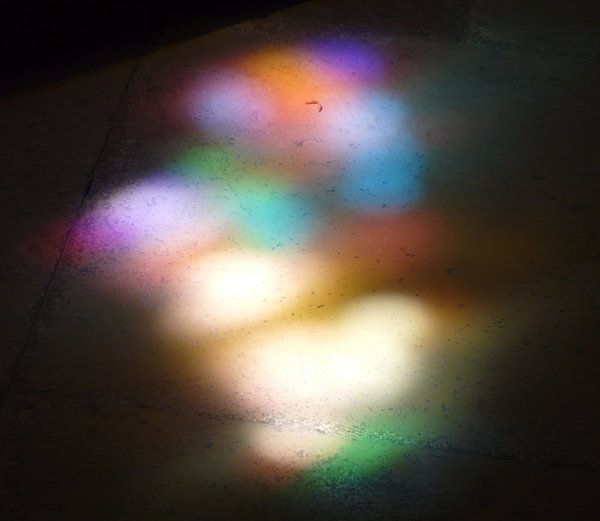
\includegraphics[height=4cm]{lichtspiel.jpg}
  \caption{A standard figure}
\end{figure}

\newtcolorbox[blend into=figures]{myfigure}[2][]{float=htb,capture=hbox,
  title={#2},every float=\centering,#1}

\begin{myfigure}{A tcolorbox figure}
  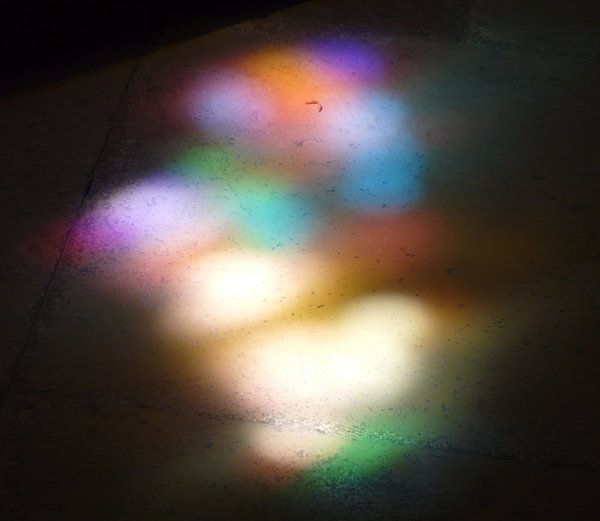
\includegraphics[height=4cm]{lichtspiel.jpg}
\end{myfigure}
\end{dispListing}
{\tcbusetemp}


\clearpage
\subsection{Lists of \texttt{tcolorbox}es}\label{sec:listsof}
For figures and tables, \LaTeX\ provides the |\listoffigures| and
|\listoftables| commands to create lists of these numbered entities.
Also, a |tcolorbox| can be part of such a kind of list.
\begin{enumerate}
\item Assign a list \meta{name} by the \emph{initialization} option
  \refKey{/tcb/new/list inside}.
\item Optionally, a new \meta{type} for list entries may be assigned
  by the \emph{initialization} option \refKey{/tcb/new/list type}.
\item List entries a generated automatically within each new |tcolorbox|
  using the above initialization.
  \begin{itemize}
  \item If \refKey{/tcb/list entry} is set, the entry is generated with it.
  \item Otherwise, if \refKey{/tcb/title} is set, the entry is generated with it.
  \item Otherwise, the entry is generated with the current number and the environment name.
  \end{itemize}
\item The generated list is displayed by \refCom{tcblistof}.
\end{enumerate}

\begin{newTcbKey}{list inside}{=\meta{name}}{no default, initially unset}
Assigns a list or contents file to the generated |tcolorbox|es.
Entries to this list are saved to a file which gets the \meta{name} as
file name extension. The list is referenced by this name in
\refCom{tcblistof}.
For example:
\begin{dispListing}
list inside=exam
\end{dispListing}
See Section \ref{listing:exercises} from page \pageref{listing:exercises}
for a complete example.
\end{newTcbKey}


\begin{newTcbKey}{list type}{=\meta{type}}{no default, initially |tcolorbox|}
Optionally, some \meta{type} can be assigned to the list entries.
For a new \meta{type}, a macro |\l@|\meta{type} has to exist which controls
the format of the list entry. The default type is defined by
\begin{dispListing}
\newcommand*\l@tcolorbox{\@dottedtocline{1}{1.5em}{2.3em}}
\end{dispListing}
This is identical to the |\l@section| setting of \LaTeX. |\l@tcolorbox| can
be redefined or a new \meta{type} can be assigned.
\end{newTcbKey}


\begin{docCommand}{tcblistof}{\oarg{macro}\marg{name}\marg{title text}}
Displays the generated list of |tcolorbox|es with the given \meta{name}.
The heading is generated by \meta{macro}\marg{title text} where \texttt{\textbackslash section}
is the default setting for \meta{macro}.\par
To display the list inside a subsection, use for example:
\begin{dispListing}
\tcblistof[\subsection]{exam}{List of Exercises}
\end{dispListing}
The result of the example is found as Subsection \ref{listofexercises} on
page \pageref{listofexercises}.
\begin{marker}
The core of the list is generated by |\@starttoc|\marg{name} which
can be wrapped into an own macro.
\end{marker}
\end{docCommand}


% !TeX root = tcolorbox.tex
% include file of tcolorbox.tex (manual of the LaTeX package tcolorbox)
\clearpage
\section{Saving and Loading of Verbatim Texts}
The following macros are slightly modified versions of the original macros
from the known packages |moreverb| and |verbatim|.
They are used implicitly inside of a |tcolorbox| environment,
but they can be used outside also.
\enlargethispage*{1.5cm}

\begin{docEnvironment}{tcbverbatimwrite}{\marg{file name}}
  Saves the \meta{environment content} to a file named by \meta{file name}.
  \TeX\ macros inside the environment are not expanded.
\begin{dispExample}
\begin{tcbverbatimwrite}{\jobname_verbexp.tex}
  This text is saved \textit{as is}.
\end{tcbverbatimwrite}

Now, we are using the file:\par
\input{\jobname_verbexp.tex}
\end{dispExample}

This environment may be used inside an own environment. Note, that inside
the environment definition |\tcbverbatimwrite| has to be used instead of
|\begin{tcbverbatimwrite}| and |\endtcbverbatimwrite| instead of |\end{tcbverbatimwrite}|.
\begin{dispExample}
\newenvironment{myverbatim}{%
  \begingroup\tcbverbatimwrite{\jobname_myverb.tex}}%
  {\endtcbverbatimwrite\endgroup}

\begin{myverbatim}
  This is the text which is saved by my own environment.
\end{myverbatim}

Now, we are using the file:\par
\input{\jobname_myverb.tex}
\end{dispExample}
\end{docEnvironment}

\begin{docEnvironment}{tcbwritetemp}{}
  Has the same function as \refEnv{tcbverbatimwrite}, but uses the key value
  of |tempfile| for the file name.
\begin{dispExample}
\begin{tcbwritetemp}
  This text is saved \textit{as is}.
\end{tcbwritetemp}

Now, we are using the file:\par
\tcbusetemp
\end{dispExample}
\end{docEnvironment}


\begin{docCommand}{tcbusetemp}{}
  Loads the current temporary file which was saved by \refEnv{tcbwritetemp}.
\end{docCommand}

% !TeX root = tcolorbox.tex
% include file of tcolorbox.tex (manual of the LaTeX package tcolorbox)
\clearpage
\section{Technical Overview and Customization}\label{sec:technical}%
\tcbset{external/prefix=external/technical_}%
This section provides a technical overview of the skin concept of |tcolorbox|.
For most applications of |tcolorbox|, one will not need to know the bells and
whistles described herein.
You may proceed to \Vref{sec:skins} where the customization options
for most users are documented.

The following explanations also cover options and settings from the \mylib{skins} library,
see  \Vref{sec:skins}.

\subsection{Skins and Drawing Engines}\label{sec:skincorekeys}
From a technical point of view, a \emph{skin} is a style definition for the
appearance of a |tcolorbox|. The core package provides some additional
option keys for skins but only two skins called \refSkin{standard}
and \refSkin{standard jigsaw}.
The \mylib{skins} library adds several more skins. To change to a skin, only one
option from the core package has to be set.

\begin{docTcbKey}{skin}{=\meta{name}}{style, no default, initially \texttt{standard}}
  Sets the current skin to \meta{name}. This is a style definition which sets all the following
  keys, i.\,e.\ for many use cases there is nothing more to do.
\begin{dispExample}
\tcbset{colback=Salmon!50!white,colframe=FireBrick!75!black,
  width=(\linewidth-8mm)/2,before=,after=\hfill,equal height group=ske}

\begin{tcolorbox}[adjusted title=My title]
  This is my content.
\end{tcolorbox}
\begin{tcolorbox}[beamer,adjusted title=My title]
  This is my content.
\end{tcolorbox}
\end{dispExample}
\end{docTcbKey}

\begin{docTcbKey}{skin first}{=\meta{name}}{style, no default, initially \texttt{standard}}
  If the box is set to be \refKey{/tcb/breakable} and \emph{is} broken actually,
  then the skin for the \emph{first} part of the break sequence
  is set to \meta{name}, see Subsection \ref{subsec:breaksequence} on page \pageref{subsec:breaksequence}.
  Typically, this key is set by a \refKey{/tcb/skin}.
\end{docTcbKey}


\begin{docTcbKey}{skin middle}{=\meta{name}}{style, no default, initially \texttt{standard}}
  If the box is set to be \refKey{/tcb/breakable} and \emph{is} broken actually,
  then the skin for the \emph{middle} parts (if any) of the break sequence
  is set to \meta{name}, see Subsection \ref{subsec:breaksequence} on page \pageref{subsec:breaksequence}.
  Typically, this key is set by a \refKey{/tcb/skin}.
\end{docTcbKey}


\begin{docTcbKey}{skin last}{=\meta{name}}{style, no default, initially \texttt{standard}}
  If the box is set to be \refKey{/tcb/breakable} and \emph{is} broken actually,
  then the skin for the \emph{last} part of the break sequence
  is set to \meta{name}, see Subsection \ref{subsec:breaksequence} on page \pageref{subsec:breaksequence}.
  Typically, this key is set by a \refKey{/tcb/skin}.
\end{docTcbKey}


\clearpage

\begin{docTcbKey}{graphical environment}{=\meta{name}}{no default, initially \texttt{pgfpicture}}
  Sets the graphical environment for the |tcolorbox| to \meta{name}.
  Feasible values are |pgfpicture| and |tikzpicture| or environments which
  inherit from one of these two. This key is set by a \refKey{/tcb/skin} and
  may seldom be used directly.
\end{docTcbKey}

The skin of a |tcolorbox| is drawn by up to four \emph{engines}.
Afterwards, the text content is drawn which is not part of a skin.
The four steps are:
\begin{enumerate}
\item The \emph{frame} of the box, drawn by \refKey{/tcb/frame engine}.
\item The \emph{interior} of the box. The interior of a box with title is
  drawn differently from a box without title.
  \refKey{/tcb/interior titled engine} or \refKey{/tcb/interior engine}
  is used to draw the interior.
\item The \emph{segmentation} (line) of the box, if there is a lower part;
  drawn by \refKey{/tcb/segmentation engine}.
\item The \emph{title area} of the box, if there is a title and
  \refKey{/tcb/title filled} is set to |true|; drawn
  by \refKey{/tcb/title engine}.
\end{enumerate}

%Every engine for the up to four steps can be set to one of the following types:
%\begin{enumerate}
%\item\docValue{standard}: the original code from the core package.
%\item\docValue{path}: a |tikz| path which can be controlled by options.
%\item\docValue{pathfirst}: a |tikz| path which can be controlled by options.
%\item\docValue{pathmiddle}: a |tikz| path which can be controlled by options.
%\item\docValue{pathlast}: a |tikz| path which can be controlled by options.
%\item\docValue{freelance}: arbitrary user code.
%\item\docValue{spartan}: a quite spartan code.
%\end{enumerate}
%\clearpage

\begin{docTcbKey}{frame engine}{=\meta{name}}{no default, initially \texttt{standard}}
  Sets the \emph{frame} drawing engine for a box to \meta{name}.
  Typically, this key is set by a \refKey{/tcb/skin}.
  Feasible values for \meta{name} are:
  \begin{itemize}
  \item\docValue{standard}: the original code from the core package,
  \item\docValue{path}: a |tikz| path which is controlled by \refKey{/tcb/frame style},
  \item\docValue{pathjigsaw}: a |tikz| path which is controlled by \refKey{/tcb/frame style},
  \item\docValue{pathfirst}: a |tikz| path which is controlled by \refKey{/tcb/frame style},
  \item\docValue{pathfirstjigsaw}: a |tikz| path which is controlled by \refKey{/tcb/frame style},
  \item\docValue{pathmiddle}: a |tikz| path which is controlled by \refKey{/tcb/frame style},
  \item\docValue{pathmiddlejigsaw}: a |tikz| path which is controlled by \refKey{/tcb/frame style},
  \item\docValue{pathlast}: a |tikz| path which is controlled by \refKey{/tcb/frame style},
  \item\docValue{pathlastjigsaw}: a |tikz| path which is controlled by \refKey{/tcb/frame style},
  \item\docValue{freelance}: deprecated.
  \item\docValue{spartan}: a quite spartan code.
  \item\docValue{empty}: draw nothing.
\end{itemize}
\end{docTcbKey}

\begin{docTcbKey}{interior titled engine}{=\meta{name}}{no default, initially \texttt{standard}}
  Sets the \emph{interior} drawing engine for a titled box to \meta{name}.
  Typically, this key is set by a \refKey{/tcb/skin}.
  Feasible values for \meta{name} are:
  \begin{itemize}
  \item\docValue{standard}: the original code from the core package,
  \item\docValue{path}: a |tikz| path which is controlled by \refKey{/tcb/interior style},
  \item\docValue{pathfirst}: a |tikz| path which is controlled by \refKey{/tcb/interior style},
  \item\docValue{pathmiddle}: a |tikz| path which is controlled by \refKey{/tcb/interior style},
  \item\docValue{pathlast}: a |tikz| path which is controlled by \refKey{/tcb/interior style},
  \item\docValue{freelance}: deprecated.
  \item\docValue{spartan}: a quite spartan code.
  \item\docValue{empty}: draw nothing.
  \end{itemize}
\end{docTcbKey}

\clearpage
\begin{docTcbKey}{interior engine}{=\meta{name}}{no default, initially \texttt{standard}}
  Sets the \emph{interior} drawing engine for an untitled box to \meta{name}.
  Typically, this key is set by a \refKey{/tcb/skin}.
  Feasible values for \meta{name} are:
  \begin{itemize}
  \item\docValue{standard}: the original code from the core package,
  \item\docValue{path}: a |tikz| path which is controlled by \refKey{/tcb/interior style},
  \item\docValue{pathfirst}: a |tikz| path which is controlled by \refKey{/tcb/interior style},
  \item\docValue{pathmiddle}: a |tikz| path which is controlled by \refKey{/tcb/interior style},
  \item\docValue{pathlast}: a |tikz| path which is controlled by \refKey{/tcb/interior style},
  \item\docValue{freelance}: deprecated.
  \item\docValue{spartan}: a quite spartan code.
  \item\docValue{empty}: draw nothing.
  \end{itemize}
\end{docTcbKey}

\begin{docTcbKey}{segmentation engine}{=\meta{name}}{no default, initially \texttt{standard}}
  Sets the \emph{segmentation} (line) drawing engine for a box to \meta{name}.
  Typically, this key is set by a \refKey{/tcb/skin}.
  Feasible values for \meta{name} are:
  \begin{itemize}
  \item\docValue{standard}: the original code from the core package,
  \item\docValue{path}: a |tikz| path which is controlled by \refKey{/tcb/segmentation style},
  \item\docValue{freelance}: deprecated.
  \item\docValue{spartan}: a quite spartan code.
  \item\docValue{empty}: draw nothing.
  \end{itemize}
\end{docTcbKey}

\begin{docTcbKey}{title engine}{=\meta{name}}{no default, initially \texttt{standard}}
  Sets the \emph{title area} drawing engine for a titled box to \meta{name}.
  Typically, this key is set by a \refKey{/tcb/skin}.
  Feasible values for \meta{name} are:
  \begin{itemize}
  \item\docValue{standard}: the original code from the core package,
  \item\docValue{path}: a |tikz| path which is controlled by \refKey{/tcb/title style},
  \item\docValue{pathfirst}: a |tikz| path which is controlled by \refKey{/tcb/title style},
  \item\docValue{pathmiddle}: a |tikz| path which is controlled by \refKey{/tcb/title style},
  \item\docValue{pathlast}: a |tikz| path which is controlled by \refKey{/tcb/title style},
  \item\docValue{freelance}: deprecated.
  \item\docValue{spartan}: a quite spartan code.
  \item\docValue{empty}: draw nothing.
  \end{itemize}
\end{docTcbKey}

\begin{marker}
After an engine is set to an initializing value, the resulting graphical
code can be changed using code option keys, see \Vref{subsec:addcodeoptions}.
\end{marker}

\clearpage
\begin{docTcbKey}{geometry nodes}{\colOpt{=true\textbar false}}{default |true|, initially |false|}
  If set to |true|, up to four |tikz| nodes are defined for a |tcolorbox|
  which are named |frame|, |interior|, |segmentation|, and |title|. These nodes
  describe the boundaries of the equally named parts of a |tcolorbox|.
  They are used by most engines based on \tikzname.
  Typically, this key is set automatically by a \refKey{/tcb/skin}.
\begin{dispExample}
\tcbset{colback=Salmon!50!white,colframe=FireBrick!75!black,
  width=(\linewidth-8mm)/2,before=,after=\hfill,equal height group=geon}

\begin{tcolorbox}[adjusted title=The title]
  The upper part.\tcblower The lower part.
\end{tcolorbox}
\begin{tcolorbox}[enhanced,adjusted title=The title,
  frame code={\path[draw=red,fill=red!25]
      (frame.south west) rectangle (frame.north east);},
  interior titled code={\path[draw=blue,fill=blue!25]
      (interior.south west) rectangle (interior.north east);},
  segmentation code={\path[draw=green,fill=green!25]
      (segmentation.south west) rectangle (segmentation.north east);},
  title code={\path[draw=black,fill=brown!75!black]
      (title.south west) rectangle (title.north east);}]
  The upper part.\tcblower The lower part.
\end{tcolorbox}
\end{dispExample}
\end{docTcbKey}






\clearpage
\subsection{Code Option Keys}\label{subsec:addcodeoptions}
The following code options are applicable for all skins.
%which
%use engines of type |freelance|.
%Especially, the skin \refSkin{freelance} supports \emph{all} of them,
%\refSkin{standard} and \refSkin{enhanced} \emph{none} of them.
The used \meta{graphical code} can be any |pgf| code. For all skins
with exception of \refSkin{standard}
and \refSkin{standard jigsaw}, the \meta{graphical code} can also
be any \tikzname\ code.


\begin{docTcbKey}{frame code}{\colOpt{=\meta{graphical code}}}{code, default from |standard|}
  The given \meta{graphical code} is used for drawing the \emph{frame} of the box.
  %This option is available only if the \refKey{/tcb/frame engine} is set to |freelance|.
\begin{dispExample}
\tcbset{colback=red!5!white,colframe=red!75!black}

\begin{tcolorbox}[enhanced,frame code={
  \foreach \n in {north east,north west,south east,south west}
  {\path [fill=red!75!black] (interior.\n) circle (3mm); }; }]
This is a \textbf{tcolorbox}.
\tcblower
This is the lower part.
\end{tcolorbox}
\end{dispExample}
\end{docTcbKey}


\begin{docTcbKey}{frame empty}{}{style, no value}
  This is a shortcut for setting  \refKey{/tcb/frame code} to empty.
  This option removes the drawing of the frame.
  Alternatively, use \refKey{/tcb/frame hidden}.
\end{docTcbKey}


\begin{docTcbKey}{interior titled code}{\colOpt{=\meta{graphical code}}}{code, default from |standard|}
  The given \meta{graphical code} is used
  for drawing the \emph{interior} of the box, if the box comes with a title.
  %This option is available only if the \refKey{/tcb/interior titled engine} is set to |freelance|.
\begin{dispExample}
\tcbset{colback=red!5!white,colframe=red!75!black,fonttitle=\bfseries}

\begin{tcolorbox}[enhanced,title=My title,interior titled code={
  \path[draw=red!5!white,line width=5mm,line cap=round]
    ([xshift=3mm,yshift=-3mm]interior.north west)
    --([xshift=-3mm,yshift=3mm]interior.south east)
    ([xshift=3mm,yshift=3mm]interior.south west)
    --([xshift=-3mm,yshift=-3mm]interior.north east);}]
This is a \textbf{tcolorbox}.
\tcblower
This is the lower part.
\end{tcolorbox}
\end{dispExample}
\end{docTcbKey}


\begin{docTcbKey}{interior titled empty}{}{style, no value}
  This is a shortcut for setting  \refKey{/tcb/interior titled code} to empty.
  This option removes the drawing of the untitled interior.
  Alternatively, use \refKey{/tcb/interior hidden}.
\end{docTcbKey}



\clearpage
\begin{docTcbKey}{interior code}{\colOpt{=\meta{graphical code}}}{code, default from |standard|}
  The given \meta{graphical code} is used
  for drawing the \emph{interior} of the box, if the box is without a title.%\\
  %This option is available only if the \refKey{/tcb/interior engine} is set to |freelance|.
\begin{dispExample}
\tcbset{colback=red!5!white,colframe=red!75!black}

\begin{tcolorbox}[enhanced,interior code={
  \path[draw=red!5!white,line width=5mm,line cap=round]
    ([xshift=3mm,yshift=-3mm]interior.north west)
    --([xshift=-3mm,yshift=3mm]interior.south east)
    ([xshift=3mm,yshift=3mm]interior.south west)
    --([xshift=-3mm,yshift=-3mm]interior.north east);}]
This is a \textbf{tcolorbox}.
\tcblower
This is the lower part.
\end{tcolorbox}
\end{dispExample}
\end{docTcbKey}

\begin{docTcbKey}{interior empty}{}{style, no value}
  This is a shortcut for setting  \refKey{/tcb/interior code} to empty.
  This option removes the drawing of the interior.
  Alternatively, use \refKey{/tcb/interior hidden}.
\end{docTcbKey}


\begin{docTcbKey}{segmentation code}{\colOpt{=\meta{graphical code}}}{code, default from |standard|}
  The given \meta{graphical code} is used for drawing the
  \emph{segmentation} area of the box.%\\
  %This option is available only if the \refKey{/tcb/segmentation engine} is set to |freelance|.
\begin{dispExample}
\tcbset{colback=red!5!white,colframe=red!75!black,fonttitle=\bfseries}

\begin{tcolorbox}[enhanced,title=My title,segmentation code={
  \path[top color=red!5!white,bottom color=red!5!white,middle color=blue]
  (segmentation.south west) rectangle (segmentation.north east);}]
This is a \textbf{tcolorbox}.
\tcblower
This is the lower part.
\end{tcolorbox}
\end{dispExample}
\end{docTcbKey}


\begin{docTcbKey}{segmentation empty}{}{style, no value}
  This is a shortcut for setting  \refKey{/tcb/segmentation code} to empty.
  This option removes the drawing of the segmentation line.
  Alternatively, use \refKey{/tcb/segmentation hidden}.
\end{docTcbKey}



\clearpage
\begin{docTcbKey}{title code}{\colOpt{=\meta{graphical code}}}{code, default from |standard|}
  The given \meta{graphical code} is used for drawing the
  \emph{title} area of the box.
  %\\
  %This option is available only if the \refKey{/tcb/title engine} is set to |freelance|.
\begin{dispExample}
\tcbset{colback=red!5!white,colframe=red!75!black,fonttitle=\bfseries,
  coltitle=black}

\begin{tcolorbox}[enhanced,title=My title,title code={
  \path[draw=yellow,solid,decorate,line width=2mm,
    decoration={coil,aspect=0,segment length=10.1mm}]
    ([xshift=1mm]title.west) -- ([xshift=-1mm]title.east);}]
This is a \textbf{tcolorbox}.
\tcblower
This is the lower part.
\end{tcolorbox}
\end{dispExample}
\end{docTcbKey}


\begin{docTcbKey}{title empty}{}{style, no value}
  This is a shortcut for setting  \refKey{/tcb/title code} to empty.
  This option removes the drawing of the title area.
  Alternatively, use \refKey{/tcb/title hidden}.
\end{docTcbKey}

\clearpage
\subsection{Subskins}\label{subsec:subskins}
A subskin is a new \refKey{/tcb/skin} based on an existing skin which
is extended or changed.

\begin{marker}
Never use geometry settings or bounding box options inside a subskin definition!
If one skin is replaced by another skin, the overall bounding box should stay
constant. Especially, if a skin is used for a breakable box, unpredictable
and unpleasant results could arise otherwise. If you want to change the
geometry also, use an additional style. See the skin \refSkin{beamer} and
the style \refKey{/tcb/beamer} as pattern.
\end{marker}

\begin{docCommand}{tcbsubskin}{\marg{name}\marg{base skin}\marg{options}}
  Creates a new skin \meta{name} which inherits all properties of an
  existing \meta{base skin} plus the given \meta{options}.
  The new skin \meta{name} can be used as value for the keys
  \refKey{/tcb/skin},
  \refKey{/tcb/skin first},
  \refKey{/tcb/skin middle}, and
  \refKey{/tcb/skin last}.
  As \meta{base skin}, one can take \refSkin{standard}, \refSkin{empty},
  \refSkin{enhanced}, or any skin from the \mylib{skins} library,
  see \Vref{sec:skins}.

\begin{dispExample}
% \tcbuselibrary{skins}
\tcbsubskin{mycross}{empty}{frame code={%
  \draw[red,line width=5pt] (frame.south west)--(frame.north east);
  \draw[red,line width=5pt] (frame.north west)--(frame.south east);},
  skin first=mycross,skin middle=mycross,skin last=mycross }

\begin{tcolorbox}[skin=mycross]
  This is my content.
\end{tcolorbox}
\end{dispExample}

\end{docCommand}


\begin{docTcbKey}{skin first is subskin of}{=\marg{base skin}\marg{options}}{no default, initially unset}
  Creates a new unnamed skin which inherits all properties of an
  existing \meta{base skin} plus the given \meta{options}.
  This skin is set as \refKey{/tcb/skin first}.\\
  See a detailed example on page~\pageref{freeboxexample}.
\end{docTcbKey}


\begin{docTcbKey}{skin middle is subskin of}{=\marg{base skin}\marg{options}}{no default, initially unset}
  Creates a new unnamed skin which inherits all properties of an
  existing \meta{base skin} plus the given \meta{options}.
  This skin is set as \refKey{/tcb/skin middle}.\\
  See a detailed example on page~\pageref{freeboxexample}.
\end{docTcbKey}


\begin{docTcbKey}{skin last is subskin of}{=\marg{base skin}\marg{options}}{no default, initially unset}
  Creates a new unnamed skin which inherits all properties of an
  existing \meta{base skin} plus the given \meta{options}.
  This skin is set as \refKey{/tcb/skin last}.\\
  See a detailed example on page~\pageref{freeboxexample}.
\end{docTcbKey}


\clearpage
\subsection{Drawing Scheme}\label{subsec:tcolorboxdrawing}

\bgroup

Depending on the complexity of a |tcolorbox| definition, the resulting box
is drawn in a more or less complex series of steps.

To document and demonstrate these drawing steps, we consider the
following box definition:

\begin{dispListing}
\newtcolorbox{testbox}[1][]{enhanced,title=Test Box,
  boxrule=1mm,titlerule=0.5mm,colframe=blue!50!black,
  interior style={top color=blue!20!green!50!white,bottom color=blue!20!yellow!50!white},
  colbacktitle=blue!50!green!90!white,segmentation style={solid},
  fonttitle=\bfseries,drop fuzzy shadow,borderline={0.3mm}{0.35mm}{yellow!50!white},
  underlay={\path[fill image opacity=0.15,fill image scale=0.9,
    fill stretch picture={\draw[blue,line width=2mm] circle (1);}]
    (interior.south west) rectangle (interior.north east);},
  watermark text={Watermark},watermark color={green!20!white},
  finish={\begin{tcbclipframe}
    \path[bottom color=black,top color=black!50!white,opacity=0.1]
      (frame.south west) -- (frame.south east) -- (frame.north east) -- cycle;
    \path[top color=white,bottom color=black!50!white,opacity=0.1]
      (frame.south west) -- (frame.north east) -- (frame.north west) -- cycle;
    \end{tcbclipframe}},#1}
\end{dispListing}
\tcbusetemp

For this definition, we get the maximal number of drawing steps:

\newtcolorbox{itembox}{oversize,enhanced,frame empty,segmentation empty,colback=white,middle=2mm,boxsep=0pt,
  fuzzy halo=0.5mm with blue!15!white,
  before lower=\raggedright\begin{itemize},after lower=\end{itemize}}

\tcbset{finishcomment/.style={
  finish={\node[fill=white,draw=black!50!white,rounded corners] at (frame.center) {#1};}
}}


\begin{itembox}
\begin{testbox}[frame empty,interior titled empty,title empty,segmentation empty,
  no shadow,no borderline,no underlay,no overlay,no finish,opacityupper=0,opacitylower=0,opacitytitle=0,
  drop fuzzy shadow=red!75!white,
  finishcomment={1.~shadow}]
\lipsum[2]
\tcblower
Lower part
\end{testbox}
\tcblower
\item Section~\ref{subsec:shadows} on page \pageref{subsec:shadows}.
\end{itembox}

\begin{itembox}
\begin{testbox}[interior titled empty,title empty,segmentation empty,
  no borderline,no underlay,no overlay,no finish,opacityupper=0,opacitylower=0,opacitytitle=0,
  colframe=red!75!white,
  finishcomment={2.~frame}]
\lipsum[2]
\tcblower
Lower part
\end{testbox}
\tcblower
\item\refKey{/tcb/colframe}, \refKey{/tcb/opacityframe}
\item\refKey{/tcb/frame code}
\item\refKey{/tcb/frame style}
\end{itembox}


\begin{itembox}
\begin{testbox}[title empty,segmentation empty,
  no borderline,no underlay,no overlay,no finish,opacityupper=0,opacitylower=0,opacitytitle=0,
  colback=red!75!white,
  finishcomment={3.~interior}]
\lipsum[2]
\tcblower
Lower part
\end{testbox}
\tcblower
\item\refKey{/tcb/colback}, \refKey{/tcb/opacityback}
\item\refKey{/tcb/interior code}, \refKey{/tcb/interior titled code}
\item\refKey{/tcb/interior style}
\end{itembox}


\begin{itembox}
\begin{testbox}[segmentation empty,
  no borderline,no underlay,no overlay,no finish,opacityupper=0,opacitylower=0,opacitytitle=0,
  colbacktitle=red!75!white,
  finishcomment={4.~title area}]
\lipsum[2]
\tcblower
Lower part
\end{testbox}
\tcblower
\item\refKey{/tcb/colbacktitle}, \refKey{/tcb/opacitybacktitle}
\item\refKey{/tcb/title code}
\item\refKey{/tcb/title style}
\end{itembox}


\begin{itembox}
\begin{testbox}[
  no borderline,no underlay,no overlay,no finish,opacityupper=0,opacitylower=0,opacitytitle=0,
  segmentation style={solid,red!75!white},
  finishcomment={5.~segmentation}]
\lipsum[2]
\tcblower
Lower part
\end{testbox}
\tcblower
\item\refKey{/tcb/lower separated}
\item\refKey{/tcb/segmentation code}
\item\refKey{/tcb/segmentation style}
\end{itembox}


\begin{itembox}
\begin{testbox}[
  no borderline,no underlay,no overlay,no finish,opacityupper=0,opacitylower=0,opacitytitle=0,
  borderline={0.3mm}{0.35mm}{red!75!white},
  finishcomment={6.~border line}]
\lipsum[2]
\tcblower
Lower part
\end{testbox}
\tcblower
\item\Vref{subsec:borderline}
\end{itembox}


\begin{itembox}
\begin{testbox}[
  no underlay,no overlay,no finish,opacityupper=0,opacitylower=0,opacitytitle=0,
  underlay={\path[opacity=0.15,fill image scale=0.9,
    fill stretch picture={\draw[red,line width=2mm] circle (1);}]
    (interior.south west) rectangle (interior.north east);},
  finishcomment={7.~underlay}]
\lipsum[2]
\tcblower
Lower part
\end{testbox}
\tcblower
\item\Vref{subsec:skinboxedtitle}
\item\Vref{subsec:skinunderlay}
\end{itembox}


\begin{itembox}
\begin{testbox}[
  no finish,opacityupper=0,opacitylower=0,opacitytitle=0,
  watermark color={red!75!white},
  finishcomment={8.~overlay}]
\lipsum[2]
\tcblower
Lower part
\end{testbox}
\tcblower
\item\Vref{subsec:overlays}
\item\Vref{subsec:watermarks}
\end{itembox}


\begin{itembox}
\begin{testbox}[
  no finish,
  colupper=red!75!white,coltitle=red!75!white,collower=red!75!white,
  finishcomment={9.~text content}]
\lipsum[2]
\tcblower
Lower part
\end{testbox}
\tcblower
\item\refKey{/tcb/colupper}, \refKey{/tcb/collower}, \refKey{/tcb/coltitle}
\item\refKey{/tcb/fontupper}, \refKey{/tcb/fontlower}, \refKey{/tcb/fonttitle}
\item\refKey{/tcb/opacityupper}, \refKey{/tcb/opacitylower}, \refKey{/tcb/opacitytitle}
\end{itembox}


\begin{itembox}
\begin{testbox}[
  finishcomment={10.~finish}]
\lipsum[2]
\tcblower
Lower part
\end{testbox}
\tcblower
\item\Vref{subsec:skinfinish}
\end{itembox}

All together, the box is drawn:
\begin{dispExample}
% \usepackage{lipsum}
\begin{testbox}
\lipsum[2]
\tcblower
Lower part
\end{testbox}
\end{dispExample}

\egroup


\clearpage
\subsection{Color Names}\label{subsec:tech_colornames}
Color settings for a |tcolorbox| are saved into named colors which may be
used inside a box, e.g. for an overlay.
\tcbdocmarginnote{\tcbdocnew{2019-01-18}}
These color names are
\begin{itemize}
\item\docColor{tcbcolframe} set by \refKey{/tcb/colframe} (frame color)
\item\docColor{tcbcolback} set by \refKey{/tcb/colback} (background color)
\item\docColor{tcbcolbacktitle} set by \refKey{/tcb/colbacktitle} (background color of the title)
\item\docColor{tcbcolbacklower} set by \refKey{/tcb/colbacklower} (skin dependend background color
  of the lower part; needs \mylib{skins} to be loaded)
\item\docColor{tcbcolupper} set by \refKey{/tcb/colupper} (text color upper part)
\item\docColor{tcbcollower} set by \refKey{/tcb/collower} (text color lower part)
\item\docColor{tcbcoltitle} set by \refKey{/tcb/coltitle} (text color title)
\end{itemize}

\medskip

\begin{dispExample}
% \tcbuselibrary{skins}
\begin{tcolorbox}[title=Color names,
    colframe=blue!50!black,colback=blue!5,
    colbacktitle=blue!50,colupper=red!35!black]
  \foreach \name in {tcbcolframe,tcbcolback,tcbcolbacktitle,tcbcolbacklower,
    tcbcolupper,tcbcollower,tcbcoltitle}
  {\tikz\path[draw,fill=\name]
    (0,0) rectangle node[right=4mm,font=\ttfamily]{\name} (0.8,0.8);\par}
\end{tcolorbox}
\end{dispExample}



\clearpage
\subsection{Useful Properties}\label{subsec:tech_properties}

The following macros describe certain \textit{properties} which may be
used for the drawing scheme, see \Fullref{subsec:tcolorboxdrawing}.
Sometimes, they are even available inside the box content. All of them are
considered to be \textit{read-only} and should never be redefined by the user.

\begin{docCommand}[doc new=2016-02-16]{tcbheightspace}{}
  If the height of a |tcolorbox| is not the natural height, the space
  difference between the forced and the natural size is hold by
  \refCom{tcbheightspace}.
  This macro is not usable inside the box content, but for skins or
  inside \refKey{/tcb/underlay}, \refKey{/tcb/overlay}, etc.

  If such a space information is needed inside the box content, see
  \refKey{/tcb/space to} instead.
\begin{dispExample}
% \tcbuselibrary{skins}
\newtcolorbox{testbox}[2][]{enhanced,size=fbox,
  colframe=blue!75!black,colback=white,height=#2,
  underlay={\node[above,inner sep=3pt] at (interior.south){%
    
\includegraphics[width=\tcbtextwidth,height=\tcbheightspace-3pt]{goldshade.png}};
    },
  #1}
\begin{testbox}{3cm}
  This is my box. The space is filled with a picture.
\end{testbox}
\begin{testbox}{2cm}
  This is my box. The space is filled with a picture.
\end{testbox}
\end{dispExample}
\end{docCommand}


\begin{docCommand}[doc new=2016-02-16]{tcbtextwidth}{}
  This property describes the box content width.
  \begin{itemize}
  \item  If there also is a lower part, it describes the width of the upper part.
  \item For \refKey{/tcb/sidebyside} boxes, it describes the combined text
    width plus segmentation.
  \item This property can be used inside the box content text with exception
    of \refKey{/tcb/fit} boxes.
  \item \refCom{tcbtextwidth} can be used for all box types for skins or
    inside \refKey{/tcb/underlay}, \refKey{/tcb/overlay}, etc.
  \end{itemize}
\begin{dispExample}
\begin{tcolorbox}[colframe=blue!75!black]
  Inside a box: \tcbtextwidth\ (=\the\linewidth).
\end{tcolorbox}
\end{dispExample}
\end{docCommand}

\pagebreak
\begin{docCommand}[doc new=2016-02-16]{tcbtextheight}{}
  This property describes the designated box content height. If the
  box is larger than the natural height, the actual content will be smaller
  than \refCom{tcbtextheight}.
  \begin{itemize}
  \item For boxes with a fixed \refKey{/tcb/height}, this property can
    be used inside the box content text. For other boxes, it denotes |0pt|
    inside the box content.
  \item \refCom{tcbtextheight} can be used for all box types for skins or
    inside \refKey{/tcb/underlay}, \refKey{/tcb/overlay}, etc.
  \end{itemize}

\begin{dispExample}
% \tcbuselibrary{skins}
\begin{tcolorbox}[enhanced,colframe=blue!75!black,
    underlay={\node[left,red] at (frame.east) {Here: \tcbtextheight};}]
  Inside a box with natural height: \tcbtextheight.
\end{tcolorbox}
\begin{tcolorbox}[enhanced,colframe=blue!75!black,height=1cm,
    underlay={\node[left,red] at (frame.east) {Here: \tcbtextheight};}]
  Inside a box with fixed height: \tcbtextheight.
\end{tcolorbox}
\end{dispExample}
\end{docCommand}


\begin{docCommand}[doc new=2017-04-25]{tcbsegmentstate}{}
  This macro contains |0|, |1|, or |2|. Itis set for every unbroken box and every broken partial box
  with the following meaning:
  \begin{itemize}
    \item\docValue{0}: The current (partial) box contains only an upper part.
    \item\docValue{1}: The current (partial) box contains an upper and a lower part.
      The segmentation node can be used for positioning.
    \item\docValue{2}: The current (partial) box contains only a lower part.
      This can only be true for parts of breakable boxes.
  \end{itemize}
  Skins like \refSkin{bicolor} use this property to paint the (partial) boxes.
\begin{dispExample}
% \tcbuselibrary{skins,raster}
\begin{tcbraster}[raster equal height,enhanced,
    watermark text=\tcbsegmentstate]
  \begin{tcolorbox}Upper part\end{tcolorbox}
  \begin{tcolorbox}Upper part\tcblower Lower part\end{tcolorbox}
\end{tcbraster}
\end{dispExample}
\end{docCommand}

% !TeX root = tcolorbox.tex
% include file of tcolorbox.tex (manual of the LaTeX package tcolorbox)
\clearpage
\section{Library \mylib{skins}}\label{sec:skins}%
\tcbset{external/prefix=external/skins_}%
The library is loaded by a package option or inside the preamble by:
\begin{dispListing}
\tcbuselibrary{skins}
\end{dispListing}
This also loads the package |tikz| \cite{tantau:2015a}. Typically but not necessarily,
the following skins use |tikz| instead of |pgf|.

\subsection{Style Option Keys}\label{subsec:addstyleoptions}
The following style options are applicable for all skins which
use engines of type |path|, |pathfirst|, |pathmiddle|, or |pathlast|.
Especially, the skin \refSkin{enhanced} supports \emph{all} of them
and \refSkin{standard} \emph{none}.

\begin{docTcbKey}{frame style}{=\meta{\texttt{\upshape tikz} keys}}{style, no default}
  The \meta{\texttt{\upshape tikz} keys} are used inside the |tikz| path command
  for drawing the \emph{frame} of the box.\\
  This option is available if the \refKey{/tcb/frame engine} is set to
  |path|, |pathfirst|, |pathmiddle|, or |pathlast|.
  It is \emph{not} available for |standard|.
\begin{exdispExample*}{frame_style}{sbs,lefthand ratio=0.66}
\tcbset{colback=red!5!white,fonttitle=\bfseries}

\begin{tcolorbox}[enhanced,title=My title,
  frame style={left color=red!75!black,
               right color=blue!75!black}]
This is a \textbf{tcolorbox}.
\tcblower
This is the lower part.
\end{tcolorbox}
\end{exdispExample*}
\end{docTcbKey}


\begin{docTcbKey}{frame style image}{=\meta{file name}}{no default, initially unset}
  Fills the frame with an external image referenced by \meta{file name}.
  For advanced features like blending of a picture with the background,
  use \refKey{/tcb/frame style} together with \refKey{/tikz/fill stretch image}.
\begin{exdispExample*}{frame_style_image}{sbs,lefthand ratio=0.66}
\tcbset{colback=red!5!white,fonttitle=\bfseries}

\begin{tcolorbox}[enhanced,title=My title,
  frame style image=blueshade.png]
This is a \textbf{tcolorbox}.
\tcblower
This is the lower part.
\end{tcolorbox}
\end{exdispExample*}
\end{docTcbKey}

\clearpage
\begin{docTcbKey}{frame style tile}{=\marg{graphics options}\marg{file name}}{no default, initially unset}
  Fills the frame with a tile pattern based on an external image referenced by \meta{file name}.
  The \meta{graphics options} are given to the underlying \docAuxCommand*{includegraphics} command.
  For advanced features like blending of a picture with the background,
  use \refKey{/tcb/frame style} together with \refKey{/tikz/fill tile image}.
\begin{exdispExample*}{frame_style_tile}{sbs,lefthand ratio=0.66}
\tcbset{colback=red!5!white,coltitle=red!30!black,
  opacityback=0.75,fonttitle=\bfseries}

\begin{tcolorbox}[enhanced,title=My title,
  frame style tile={width=1cm}{pink_marble.png}]
This is a \textbf{tcolorbox}.
\tcblower
This is the lower part.
\end{tcolorbox}
\end{exdispExample*}
\end{docTcbKey}


\begin{docTcbKey}{frame hidden}{}{style, no value}
  This is a shortcut for |frame style={draw=none,fill=none}|.
  Depending on the skin, this option switches off the drawing of the
  frame.
  Alternatively, use \refKey{/tcb/frame empty}.
\begin{exdispExample*}{frame_hidden}{sbs,lefthand ratio=0.66}
\tcbset{colback=red!5!white,colframe=red!75!black,
  fonttitle=\bfseries,coltitle=black}

\begin{tcolorbox}[enhanced,title=My title,
  frame hidden]
This is a \textbf{tcolorbox}.
\tcblower
This is the lower part.
\end{tcolorbox}
\end{exdispExample*}
\end{docTcbKey}


\begin{docTcbKey}{interior style}{=\meta{\texttt{\upshape tikz} keys}}{style, no default}
  The \meta{\texttt{\upshape tikz} keys} are used inside the |tikz| path command
  for drawing the \emph{interior} of the box. They are used for the titled
  and for the untitled version as well.\\
  This option is available if the \refKey{/tcb/interior titled engine}
  or \refKey{/tcb/interior engine} is set to
  |path|, |pathfirst|, |pathmiddle|, or |pathlast|.
  It is \emph{not} available for |standard|.
\begin{exdispExample*}{interior_style}{sbs,lefthand ratio=0.66}
\tcbset{colframe=red!75!black,fonttitle=\bfseries}

\begin{tcolorbox}[enhanced,title=My title,
  interior style={left color=red!20!white,
                  right color=yellow!50!white}]
This is a \textbf{tcolorbox}.
\tcblower
This is the lower part.
\end{tcolorbox}
\end{exdispExample*}
\end{docTcbKey}

\clearpage
\begin{docTcbKey}{interior style image}{=\meta{file name}}{no default, initially unset}
  Fills the interior with an external image referenced by \meta{file name}.
  For advanced features like blending of a picture with the background,
  use \refKey{/tcb/interior style} together with \refKey{/tikz/fill stretch image}.
\begin{exdispExample*}{interior_style_image}{sbs,lefthand ratio=0.66}
\tcbset{colframe=red!75!black,fonttitle=\bfseries}

\begin{tcolorbox}[enhanced,title=My title,
  interior style image=goldshade.png]
This is a \textbf{tcolorbox}.
\tcblower
This is the lower part.
\end{tcolorbox}
\end{exdispExample*}
\end{docTcbKey}


\begin{docTcbKey}{interior style tile}{=\marg{graphics options}\marg{file name}}{no default, initially unset}
  Fills the interior with a tile pattern based on an external image referenced by \meta{file name}.
  The \meta{graphics options} are given to the underlying \docAuxCommand*{includegraphics} command.
  For advanced features like blending of a picture with the background,
  use \refKey{/tcb/interior style} together with \refKey{/tikz/fill tile image}.

\begin{exdispExample*}{interior_style_tile}{sbs,lefthand ratio=0.66}
\tcbset{colframe=red!75!black,fonttitle=\bfseries}

\begin{tcolorbox}[enhanced,title=My title,
  interior style tile={width=2cm}{crinklepaper.png}]
This is a \textbf{tcolorbox}.
\tcblower
This is the lower part.
\end{tcolorbox}
\end{exdispExample*}
\end{docTcbKey}


\begin{docTcbKey}{interior hidden}{}{style, no value}
  This is a shortcut for |interior style={draw=none,fill=none}|.
  Depending on the skin, this option switches off the drawing of the
  interior.
  Alternatively, use \refKey{/tcb/interior empty} and/or \refKey{/tcb/interior titled empty}.
\begin{exdispExample*}{interior_hidden}{sbs,lefthand ratio=0.66}
\tcbset{frame style={top color=red!20!white,
  bottom color=red!20!white!75!black},
  fonttitle=\bfseries,coltitle=black}

\begin{tcolorbox}[enhanced,title=My title,
  interior hidden]
This is a \textbf{tcolorbox}.
\tcblower
This is the lower part.
\end{tcolorbox}
\end{exdispExample*}
\end{docTcbKey}

\clearpage
\begin{docTcbKey}{segmentation style}{=\meta{\texttt{\upshape tikz} keys}}{style, no default}
  The \meta{\texttt{\upshape tikz} keys} are used inside the |tikz| path command
  for drawing the \emph{segmentation} line of the box.\\
  This option is available if the \refKey{/tcb/segmentation engine}
  is set to |path|.
  It is \emph{not} available for |standard|.
\begin{exdispExample*}{segmentation_style}{sbs,lefthand ratio=0.66}
\tcbset{colback=red!5!white,colframe=red!75!black,
  fonttitle=\bfseries}

\begin{tcolorbox}[enhanced,title=My title,
  segmentation style={double=white,draw=blue,
                  double distance=1pt,solid}]
This is a \textbf{tcolorbox}.
\tcblower
This is the lower part.
\end{tcolorbox}
\end{exdispExample*}
\end{docTcbKey}


\begin{docTcbKey}{segmentation hidden}{}{style, no value}
  This is a shortcut for |segmentation style={draw=none,fill=none}|.
  Depending on the skin, this option switches off the drawing of the
  segmentation line. See also \refKey{/tcb/lower separated} which
  has the same effect for most skins.
  Alternatively, use \refKey{/tcb/segmentation empty}.
\begin{exdispExample*}{segmentation_hidden}{sbs,lefthand ratio=0.66}
\tcbset{colback=red!5!white,colframe=red!75!black,
  fonttitle=\bfseries}

\begin{tcolorbox}[title=My title,
  enhanced,segmentation hidden]
This is a \textbf{tcolorbox}.
\tcblower
This is the lower part.
\end{tcolorbox}
\end{exdispExample*}
\end{docTcbKey}


\begin{docTcbKey}{title style}{=\meta{\texttt{\upshape tikz} keys}}{style, no default}
  The \meta{\texttt{\upshape tikz} keys} are used inside the |tikz| path command
  for drawing the \emph{title area} of the box.\\
  This option is available if the \refKey{/tcb/title engine} is set to
  |path|, |pathfirst|, |pathmiddle|, or |pathlast|.
  It is \emph{not} available for |standard|.
\begin{exdispExample*}{title_style}{sbs,lefthand ratio=0.66}
\tcbset{colback=red!5!white,colframe=red!75!black,
  coltitle=blue!50!black,fonttitle=\bfseries}

\begin{tcolorbox}[enhanced,title=My title,
  title style={left color=blue!15!yellow,
               right color=red!85!black}]
This is a \textbf{tcolorbox}.
\tcblower
This is the lower part.
\end{tcolorbox}
\end{exdispExample*}
\end{docTcbKey}

\clearpage
\begin{docTcbKey}{title style image}{=\meta{file name}}{no default, initially unset}
  Fills the title area with an external image referenced by \meta{file name}.
  For advanced features like blending of a picture with the background,
  use \refKey{/tcb/title style} together with \refKey{/tikz/fill stretch image}.

\begin{exdispExample*}{title_style_image}{sbs,lefthand ratio=0.66}
\tcbset{colback=blue!5!white,colframe=blue!75!black,
  fonttitle=\bfseries}

\begin{tcolorbox}[enhanced,title=My title,
  title style image=blueshade.png]
This is a \textbf{tcolorbox}.
\tcblower
This is the lower part.
\end{tcolorbox}
\end{exdispExample*}
\end{docTcbKey}


\begin{docTcbKey}{title style tile}{=\marg{graphics options}\marg{file name}}{no default, initially unset}
  Fills the title area with a tile pattern based on an external image referenced by \meta{file name}.
  The \meta{graphics options} are given to the underlying \docAuxCommand*{includegraphics} command.
  For advanced features like blending of a picture with the background,
  use \refKey{/tcb/title style} together with \refKey{/tikz/fill tile image}.

\begin{exdispExample*}{title_style_tile}{sbs,lefthand ratio=0.66}
\tcbset{colback=red!5!white,colframe=red!75!black,
  coltitle=blue!50!black,fonttitle=\bfseries}

\begin{tcolorbox}[enhanced,title=My title,
  title style tile={width=1cm}{pink_marble.png}]
This is a \textbf{tcolorbox}.
\tcblower
This is the lower part.
\end{tcolorbox}
\end{exdispExample*}
\end{docTcbKey}


\begin{docTcbKey}{title hidden}{}{style, no value}
  This is a shortcut for |title style={draw=none,fill=none}|.
  Depending on the skin, this option switches off the drawing of the
  title background. See also \refKey{/tcb/title filled} for a similar effect.
  Alternatively, use \refKey{/tcb/title empty}.
\begin{exdispExample*}{title_hidden}{sbs,lefthand ratio=0.66}
\tcbset{colback=red!5!white,colframe=red!75!black,
  fonttitle=\bfseries}

\begin{tcolorbox}[title=My title,
  enhanced,title hidden]
This is a \textbf{tcolorbox}.
\tcblower
This is the lower part.
\end{tcolorbox}
\end{exdispExample*}
\end{docTcbKey}


\clearpage


\begin{docTcbKey}[][doc new=2015-01-14]{titlerule style}{=\meta{\texttt{\upshape tikz} keys}}{style, no default}
  The \meta{\texttt{\upshape tikz} keys} are used to draw a title rule,
  i.e.\ a rule below the optional title. The width of the rule is controlled
  by \refKey{/tcb/titlerule}. It may be set directly to a smaller width
  to create mixed effects with the standard rule.
  This option is implemented as an \refKey{/tcb/underlay}. Thus, it is not
  available for \refSkin{standard} and \refSkin{standard jigsaw}, but for
  all other skins, e.g.\ \refSkin{enhanced}.
  As an underlay, this option can be used multiple times and is removed
  by \refKey{/tcb/no underlay}.
\begin{exdispExample*}{titlerule_style_1}{sbs,lefthand ratio=0.66}
\begin{tcolorbox}[enhanced,
  colback=red!5!white,colframe=red!75!black,
  colbacktitle=red!50!yellow,fonttitle=\bfseries,
  title=My title,
  titlerule=1mm,
  titlerule style=yellow  ]
This is a \textbf{tcolorbox}.
\end{tcolorbox}
\end{exdispExample*}

\begin{exdispExample*}{titlerule_style_2}{sbs,lefthand ratio=0.66}
\begin{tcolorbox}[enhanced,
  colback=red!5!white,colframe=red!75!black,
  colbacktitle=red!50!yellow,fonttitle=\bfseries,
  title=My title,
  titlerule=1mm,
  titlerule style={yellow,line width=0.5mm}  ]
This is a \textbf{tcolorbox}.
\end{tcolorbox}
\end{exdispExample*}

\begin{exdispExample*}{titlerule_style_3}{sbs,lefthand ratio=0.66}
\begin{tcolorbox}[enhanced,
  colback=red!10!white,colframe=red!75!black,
  colbacktitle=red!50!yellow,fonttitle=\bfseries,
  frame hidden,
  title=My title,
  boxrule=0pt,titlerule=1mm,
  titlerule style=red!50!black  ]
This is a \textbf{tcolorbox}.
\end{tcolorbox}
\end{exdispExample*}

\begin{exdispExample*}{titlerule_style_4}{sbs,lefthand ratio=0.66}
%\usetikzlibrary{arrows.meta}
\begin{tcolorbox}[empty,
  coltitle=red!75!black,fonttitle=\bfseries,
  borderline horizontal={0.5mm}{0pt}{red!50!white},
  title=My title,
  titlerule style={red,
    arrows = {Hooks[arc=270]-Hooks[arc=270]}} ]
This is a \textbf{tcolorbox}.
\end{tcolorbox}
\end{exdispExample*}
\end{docTcbKey}

\clearpage

The combined \tikzname\ style applied to frame, interior, and title
background can used by authors in customizing code.

\begin{docTikzKey}{tcb fill frame}{}{style, no value}
This is a \tikzname\ style which is finally applied to the \emph{frame}
of the box.

\begin{exdispExample*}{tcb_fill_frame}{sbs,lefthand ratio=0.66}
% \tcbuselibrary{hooks}
\tcbset{enhanced,colback=red!5!white,
  colframe=red!75!black,fonttitle=\bfseries,
  frame code app={\path[tcb fill frame]
    ([yshift=-2mm]frame.north)
        circle (8mm); }  }

\begin{tcolorbox}[title=My title]
This is a \textbf{tcolorbox}.
\tcblower
This is the lower part.
\end{tcolorbox}
\end{exdispExample*}
\end{docTikzKey}


\begin{docTikzKey}{tcb fill interior}{}{style, no value}
This is a \tikzname\ style which is finally applied to the \emph{interior}
of the box.

\begin{exdispExample*}{tcb_fill_interior}{sbs,lefthand ratio=0.66}
% \tcbuselibrary{hooks}
\tcbset{enhanced,colback=red!5!white,
  colframe=red!75!black,fonttitle=\bfseries,
  interior titled code app={\path[tcb fill interior]
      ([yshift=-0.1pt]interior.north east)
    --([yshift=3pt]interior.north)
    --([yshift=-0.1pt]interior.north west)
    --cycle;}  }

\begin{tcolorbox}[title=My title]
This is a \textbf{tcolorbox}.
\tcblower
This is the lower part.
\end{tcolorbox}
\end{exdispExample*}
\end{docTikzKey}


\begin{docTikzKey}{tcb fill title}{}{style, no value}
This is a \tikzname\ style which is finally applied to the \emph{title area}
of the box.

\begin{exdispExample*}{tcb_fill_title}{sbs,lefthand ratio=0.66}
% \tcbuselibrary{hooks}
\tcbset{enhanced,colback=red!5!white,
  colframe=red!75!black,fonttitle=\bfseries,
  colbacktitle=blue!75!black,
  title code app={\path[tcb fill title]
    (title) circle (5mm); }  }

\begin{tcolorbox}[title=My title]
This is a \textbf{tcolorbox}.
\tcblower
This is the lower part.
\end{tcolorbox}
\end{exdispExample*}
\end{docTikzKey}


\clearpage
\subsection{Boxed Title Option Keys}\label{subsec:skinboxedtitle}

\subsubsection{Boxed Title Placement}
The following options place the title text into an own \refCom{tcbox}.
This boxed title can be customized independently from the main box using
\refKey{/tcb/boxed title style}.
The placement can be influenced by \meta{boxtitle options}.

\begin{docTcbKey}{attach boxed title to top left}{\colOpt{=\marg{boxtitle options}}}{style, default empty}
The title is boxed with a \refCom{tcbox} and attached to
the top left corner of the main box.
\begin{exdispExample*}{attach_boxed_title_to_top_left}{sbs,lefthand ratio=0.66}
\begin{tcolorbox}[enhanced,title=My title,
  attach boxed title to top left]
  This is a \textbf{tcolorbox}.
\end{tcolorbox}
\end{exdispExample*}
\end{docTcbKey}

\begin{docTcbKey}{attach boxed title to top center}{\colOpt{=\marg{boxtitle options}}}{style, default empty}
The title is boxed with a \refCom{tcbox} and attached to
the top of the main box.
\begin{exdispExample*}{attach_boxed_title_to_top_center}{sbs,lefthand ratio=0.66}
\begin{tcolorbox}[enhanced,title=My title,
  attach boxed title to top center]
  This is a \textbf{tcolorbox}.
\end{tcolorbox}
\end{exdispExample*}
\end{docTcbKey}

\begin{docTcbKey}{attach boxed title to top right}{\colOpt{=\marg{boxtitle options}}}{style, default empty}
The title is boxed with a \refCom{tcbox} and attached to
the top right corner of the main box.
\begin{exdispExample*}{attach_boxed_title_to_top_right}{sbs,lefthand ratio=0.66}
\begin{tcolorbox}[enhanced,title=My title,
  attach boxed title to top right]
  This is a \textbf{tcolorbox}.
\end{tcolorbox}
\end{exdispExample*}
\end{docTcbKey}

\begin{docTcbKey}{attach boxed title to bottom left}{\colOpt{=\marg{boxtitle options}}}{style, default empty}
The title is boxed with a \refCom{tcbox} and attached to
the bottom left corner of the main box.
\begin{exdispExample*}{attach_boxed_title_to_bottom_left}{sbs,lefthand ratio=0.66}
\begin{tcolorbox}[enhanced,title=My title,
  attach boxed title to bottom left]
  This is a \textbf{tcolorbox}.
\end{tcolorbox}
\end{exdispExample*}
\end{docTcbKey}

\begin{docTcbKey}{attach boxed title to bottom center}{\colOpt{=\marg{boxtitle options}}}{style, default empty}
The title is boxed with a \refCom{tcbox} and attached to
the bottom of the main box.
\begin{exdispExample*}{attach_boxed_title_to_bottom_center}{sbs,lefthand ratio=0.66}
\begin{tcolorbox}[enhanced,title=My title,
  attach boxed title to bottom center]
  This is a \textbf{tcolorbox}.
\end{tcolorbox}
\end{exdispExample*}
\end{docTcbKey}

\begin{docTcbKey}{attach boxed title to bottom right}{\colOpt{=\marg{boxtitle options}}}{style, default empty}
The title is boxed with a \refCom{tcbox} and attached to
the bottom right corner of the main box.
\begin{exdispExample*}{attach_boxed_title_to_bottom_right}{sbs,lefthand ratio=0.66}
\begin{tcolorbox}[enhanced,title=My title,
  attach boxed title to bottom right]
  This is a \textbf{tcolorbox}.
\end{tcolorbox}
\end{exdispExample*}
\end{docTcbKey}


\clearpage
\begin{docTcbKey}[][doc new=2016-02-26]{attach boxed title to top}{\colOpt{=\marg{boxtitle options}}}{style, default empty}
  This is a convenient style to mimic a standard title.
  It uses \refKey{/tcb/attach boxed title to top center},
  \refKey{/tcb/minipage boxed title}, and sizes the boxed title to match
  the base box.
\begin{dispExample*}{sbs,lefthand ratio=0.66}
\begin{tcolorbox}[enhanced,title=My title,
  attach boxed title to top,
  boxed title style={colframe=red}]
  This is a \textbf{tcolorbox}.
\end{tcolorbox}
\end{dispExample*}
\end{docTcbKey}

\begin{docTcbKey}[][doc new=2016-02-26]{attach boxed title to top*}{\colOpt{=\marg{boxtitle options}}}{style, default empty}
  In contrast to \refKey{/tcb/attach boxed title to top}, this style
  uses smaller left and right rules to avoid previewer glitches.
  Typically, one would not use different colors for the frame as in the
  example below.
\begin{dispExample*}{sbs,lefthand ratio=0.66}
\begin{tcolorbox}[enhanced,title=My title,
  attach boxed title to top*,
  boxed title style={colframe=red}]
  This is a \textbf{tcolorbox}.
\end{tcolorbox}
\end{dispExample*}
\end{docTcbKey}

\begin{docTcbKey}[][doc new=2016-02-26]{attach boxed title to bottom}{\colOpt{=\marg{boxtitle options}}}{style, default empty}
  This is a convenient style to produce a standard-like title at the bottom
  of the box.
  It uses \refKey{/tcb/attach boxed title to bottom center},
  \refKey{/tcb/minipage boxed title}, and sizes the boxed title to match
  the base box.
\begin{dispExample*}{sbs,lefthand ratio=0.66}
\begin{tcolorbox}[enhanced,title=My title,
  attach boxed title to bottom,
  boxed title style={colframe=red}]
  This is a \textbf{tcolorbox}.
\end{tcolorbox}
\end{dispExample*}
\end{docTcbKey}

\begin{docTcbKey}[][doc new=2016-02-26]{attach boxed title to bottom*}{\colOpt{=\marg{boxtitle options}}}{style, default empty}
  In contrast to \refKey{/tcb/attach boxed title to top}, this style
  uses smaller left and right rules to avoid previewer glitches.
\begin{dispExample*}{sbs,lefthand ratio=0.66}
\begin{tcolorbox}[enhanced,title=My title,
  attach boxed title to bottom*]
  This is a \textbf{tcolorbox}.
\end{tcolorbox}
\end{dispExample*}
\end{docTcbKey}

\begin{docTcbKey}[][doc new=2016-02-26]{flip title}{\colOpt{=\marg{options}}}{style, default empty}
  This style combines \refKey{/tcb/attach boxed title to bottom*}
  with \refKey{/tcb/boxed title style}. The \meta{options} are given to
  \refKey{/tcb/boxed title style}.
\begin{dispExample*}{sbs,lefthand ratio=0.66}
\begin{tcolorbox}[tile,flip title={sharp corners},
  title=My title,colback=red!10,
  colbacktitle=red!75!black]
  This is a \textbf{tcolorbox}.
\end{tcolorbox}
\end{dispExample*}
\end{docTcbKey}

\clearpage

\subsubsection{Options for the Boxed Title Placement}
The \meta{boxtitle options} of the keys described above are shift values.
The dimensions of the boxed title are stored into two macros
\docAuxCommand{tcboxedtitleheight} and
\docAuxCommand{tcboxedtitlewidth}. These macros can be used inside the
following \meta{boxtitle options}:

\begin{boxTcbKey}{xshift}{=\meta{length}}{no default, initially |0pt|}
The boxed title is shifted by \meta{length} in the horizontal direction.
\begin{exdispExample*}{xshift}{sbs,lefthand ratio=0.66}
\begin{tcolorbox}[enhanced,title=My title,
  attach boxed title to top left={xshift=-2mm},
  boxed title style={size=small,colback=blue}]
  This is a \textbf{tcolorbox}.
\end{tcolorbox}
\end{exdispExample*}
\end{boxTcbKey}

\begin{boxTcbKey}{yshift}{=\meta{length}}{no default, initially |0pt|}
The boxed title is shifted by \meta{length} in the vertical direction.
\begin{exdispExample*}{yshift}{sbs,lefthand ratio=0.66}
\begin{tcolorbox}[enhanced,title=My title,
  attach boxed title to top center=
    {yshift=-\tcboxedtitleheight/2},
  boxed title style={size=small,colback=blue}]
  This is a \textbf{tcolorbox}.
\end{tcolorbox}
\end{exdispExample*}
\end{boxTcbKey}

\begin{boxTcbKey}{yshifttext}{=\meta{length}}{no default, initially |0pt|}
The text inside the main box by \meta{length} to give room for e.\,g.\ a sunken title.
\begin{exdispExample*}{yshifttext}{sbs,lefthand ratio=0.66}
\begin{tcolorbox}[enhanced,title=My title,
  attach boxed title to top center=
    {yshift=-3mm,yshifttext=-1mm},
  boxed title style={size=small,colback=blue}]
  This is a \textbf{tcolorbox}.
\end{tcolorbox}
\end{exdispExample*}
\end{boxTcbKey}

\begin{boxTcbKey}{yshift*}{=\meta{length}}{no default, initially |0pt|}
Sets \refKey{/tcb/boxtitle/yshift} and \refKey{/tcb/boxtitle/yshifttext}
the same time.\\
\refKey{/tcb/boxtitle/yshifttext} is only set if necessary.
\begin{exdispExample*}{yshiftstar}{sbs,lefthand ratio=0.66}
\begin{tcolorbox}[enhanced,title=My title,
  attach boxed title to top center={yshift*=-3mm},
  boxed title style={size=small,colback=blue}]
  This is a \textbf{tcolorbox}.
\end{tcolorbox}
\end{exdispExample*}
\end{boxTcbKey}

\begin{marker}
The bounding box of the resulting total |tcolorbox| is adapted automatically to the
\emph{vertical} dimensions of the boxed title. Possible horizontal enlargements
are \emph{not} automatically computed.
\end{marker}


\begin{exdispExample*}{boxed_title_example_1}{sbs,lefthand ratio=0.66}
\begin{tcolorbox}[enhanced,title=My title,
  attach boxed title to top left=
    {xshift=-2mm,yshift=-2mm},
  boxed title style={size=small,colback=blue},
  show bounding box]
  This is a \textbf{tcolorbox}.
\end{tcolorbox}
\end{exdispExample*}


\clearpage
\subsubsection{Options for the Boxed Title Box}
\begin{marker}
  The boxed title options are implemented as an underlay, see \Vref{subsec:skinunderlay}.
  Therefore, a boxed title is not drawn, if a skin does not support underlays
  like \refSkin{standard}. Still, the room for the boxed
  titles gets reserved in these cases.
\end{marker}

\begin{marker}
  A \tikzname\ node |title| is produced by a boxed title which can be used
  inside \refKey{/tcb/frame code}, \refKey{/tcb/interior code},
  underlays, overlays, and finishes.
\end{marker}

\begin{marker}
  A boxed title is almost always the first underlay. The only exceptions are
  underlays defined by \refKey{/tcb/underlay boxed title} which are drawn
  before. Additionally, underlays defined by \refKey{/tcb/underlay boxed title}
  are only drawn, if a boxed title is actually set. They are ignored, if
  there is no boxed title.
\end{marker}



\begin{docTcbKey}[][doc new=2016-02-26]{boxed title size}{=\meta{size}}{no default, initially |title|}
  This setting defines the basic size for the title box. Further settings
  can be applied using \refKey{/tcb/boxed title style}.
  Feasible values for \meta{size} are:
  \begin{itemize}
  \item\docValue{title}: Sets the size according to \refKey{/tcb/size}|=|\docValue{title}.
  \item\docValue{standard}: No size setting. Typically, this is identical to
    \refKey{/tcb/size}|=|\docValue{normal}.
  \item\docValue{copy}: The size values for a title of the base box are copied
    for the title box.
  \end{itemize}

\begin{dispExample}
% \tcbuselibrary{raster}
\begin{tcbraster}[raster columns=3,enhanced,boxrule=0.4pt,
    title=My title,attach boxed title to top center]
  \begin{tcolorbox}[boxed title size=title]
    This is a \textbf{tcolorbox}.
  \end{tcolorbox}
  \begin{tcolorbox}[boxed title size=standard]
    This is a \textbf{tcolorbox}.
  \end{tcolorbox}
  \begin{tcolorbox}[boxed title size=copy]
    This is a \textbf{tcolorbox}.
  \end{tcolorbox}
\end{tcbraster}
\end{dispExample}

\end{docTcbKey}


\clearpage
\begin{docTcbKey}[][doc updated=2016-02-26]{boxed title style}{=\meta{options}}{style, initially empty}
By default, a boxed title is dimensioned with \refKey{/tcb/size}|=|\docValue*{title}
and inherits the \refKey{/tcb/skin} and \refKey{/tcb/colframe} of the main box.
Also, the \refKey{/tcb/colback} is inherited from the main \refKey{/tcb/colbacktitle}.
Font and color of the title text are set as usual.
All other \meta{options} are set by the \refKey{/tcb/boxed title style} key.
Since a boxed title is set by \refCom{tcbox}, all |tcolorbox| options are
applicable here. If \refKey{/tcb/boxed title style} is used several times,
the \meta{options} are is appended.

\begin{exdispExample*}{boxed_title_style_1}{sbs,lefthand ratio=0.66}
\begin{tcolorbox}[enhanced,title=My title,
  fonttitle=\bfseries,coltitle=green!25!black,
  attach boxed title to top center=
    {yshift=-2mm,yshifttext=-1mm},
  boxed title style={colframe=green!75!black,
    colback=yellow!50!green}]
  This is a \textbf{tcolorbox}.
\end{tcolorbox}
\end{exdispExample*}


\begin{exdispExample*}{boxed_title_style_2}{sbs,lefthand ratio=0.66}
\begin{tcolorbox}[enhanced,title=My title,
  colframe=red!50!black,colback=red!10!white,
  arc=1mm,colbacktitle=red!10!white,
  fonttitle=\bfseries,coltitle=red!50!black,
  attach boxed title to top left=
    {xshift=3.2mm,yshift=-0.50mm},
  boxed title style={skin=enhancedfirst jigsaw,
    size=small,arc=1mm,bottom=-1mm,
    interior style={fill=none,
      top color=red!30!white,
      bottom color=red!20!white}}]
  This is a \textbf{tcolorbox}.
\end{tcolorbox}
\end{exdispExample*}

\begin{exdispExample}{boxed_title_style_3}
\begin{tcolorbox}[enhanced,title=My title,
  colframe=blue!50!black,colback=blue!10!white,colbacktitle=blue!5!yellow!10!white,
  fonttitle=\bfseries,coltitle=black,attach boxed title to top center=
    {yshift=-0.25mm-\tcboxedtitleheight/2,yshifttext=2mm-\tcboxedtitleheight/2},
  boxed title style={boxrule=0.5mm,
    frame code={ \path[tcb fill frame] ([xshift=-4mm]frame.west)
    -- (frame.north west) -- (frame.north east) -- ([xshift=4mm]frame.east)
    -- (frame.south east) -- (frame.south west) -- cycle; },
    interior code={ \path[tcb fill interior] ([xshift=-2mm]interior.west)
    -- (interior.north west) -- (interior.north east)
    -- ([xshift=2mm]interior.east) -- (interior.south east) -- (interior.south west)
    -- cycle;}  }]
  \lipsum[2]
\end{tcolorbox}
\end{exdispExample}


\begin{exdispExample}{boxed_title_style_4}
% \usepackage{varwidth}
\newtcolorbox{mybox}[2][]{enhanced,skin=enhancedlast jigsaw,
  attach boxed title to top left={xshift=-4mm,yshift=-0.5mm},
  fonttitle=\bfseries\sffamily,varwidth boxed title=0.7\linewidth,
  colbacktitle=blue!45!white,colframe=red!50!black,
  interior style={top color=blue!10!white,bottom color=red!10!white},
  boxed title style={empty,arc=0pt,outer arc=0pt,boxrule=0pt},
  underlay boxed title={
    \fill[blue!45!white] (title.north west) -- (title.north east)
      -- +(\tcboxedtitleheight-1mm,-\tcboxedtitleheight+1mm)
      -- ([xshift=4mm,yshift=0.5mm]frame.north east) -- +(0mm,-1mm)
      -- (title.south west) -- cycle;
    \fill[blue!45!white!50!black] ([yshift=-0.5mm]frame.north west)
      -- +(-0.4,0) -- +(0,-0.3) -- cycle;
    \fill[blue!45!white!50!black] ([yshift=-0.5mm]frame.north east)
      -- +(0,-0.3) -- +(0.4,0) -- cycle;  },
  title={#2},#1}

\begin{mybox}{My title}
  \lipsum[2]
\end{mybox}
\end{exdispExample}


\begin{exdispExample}{boxed_title_style_5}
% \usepackage{varwidth}
\newtcolorbox{mybox}[2][]{enhanced,
  attach boxed title to top left={xshift=1cm,yshift=-2mm},
  fonttitle=\bfseries,varwidth boxed title=0.7\linewidth,
  colbacktitle=green!45!white,coltitle=green!10!black,colframe=green!50!black,
  interior style={top color=yellow!10!white,bottom color=green!10!white},
  boxed title style={boxrule=0.75mm,colframe=white,
    borderline={0.1mm}{0mm}{green!50!black},
    borderline={0.1mm}{0.75mm}{green!50!black},
    interior style={top color=green!10!white,bottom color=green!10!white,
      middle color=green!50!white},
    drop fuzzy shadow},
  title={#2},#1}

\begin{mybox}{My title}
  \lipsum[2]
\end{mybox}
\end{exdispExample}


\begin{exdispExample}{boxed_title_style_6}
\newtcolorbox{flipbox}[2][]{
  enhanced,colframe=blue!50!black,colback=yellow!5,fonttitle=\bfseries,
  flip title={interior hidden},title={#2},#1}

\begin{flipbox}{My title}
\lipsum[2]
\end{flipbox}
\end{exdispExample}


\begin{exdispExample}{boxed_title_style_7}
% \usepackage{varwidth}
\newtcolorbox{mybox}[2][]{skin=enhancedlast jigsaw,interior hidden,
  boxsep=0pt,top=0pt,colframe=red,coltitle=red!50!black,
  fonttitle=\bfseries\sffamily,
  attach boxed title to bottom center,
  boxed title style={empty,boxrule=0.5mm},
  varwidth boxed title=0.5\linewidth,
  underlay boxed title={
    \draw[white,line width=0.5mm]
      ([xshift=0.3mm-\tcboxedtitleheight*2,yshift=0.3mm]title.north west)
      --([xshift=-0.3mm+\tcboxedtitleheight*2,yshift=0.3mm]title.north east);
    \path[draw=red,top color=white,bottom color=red!50!white,line width=0.5mm]
    ([xshift=0.25mm-\tcboxedtitleheight*2,yshift=0.25mm]title.north west)
    cos +(\tcboxedtitleheight,-\tcboxedtitleheight/2)
    sin +(\tcboxedtitleheight,-\tcboxedtitleheight/2)
    -- ([xshift=0.25mm,yshift=0.25mm]title.south west)
    -- ([yshift=0.25mm]title.south east)
    cos +(\tcboxedtitleheight,\tcboxedtitleheight/2)
    sin +(\tcboxedtitleheight,\tcboxedtitleheight/2); },
  title={#2},#1}

\begin{mybox}{My title}
  \lipsum[2]
\end{mybox}
\end{exdispExample}


\begin{exdispExample}{boxed_title_style_8}
% \usepackage{varwidth}
\newtcolorbox{mybox}[2][]{enhanced,
  before skip=2mm,after skip=2mm,
  colback=black!5,colframe=black!50,boxrule=0.2mm,
  attach boxed title to top left={xshift=1cm,yshift*=1mm-\tcboxedtitleheight},
  varwidth boxed title*=-3cm,
  boxed title style={frame code={
    \path[fill=tcbcol@back!30!black]
      ([yshift=-1mm,xshift=-1mm]frame.north west)
        arc[start angle=0,end angle=180,radius=1mm]
      ([yshift=-1mm,xshift=1mm]frame.north east)
        arc[start angle=180,end angle=0,radius=1mm];
    \path[left color=tcbcol@back!60!black,right color=tcbcol@back!60!black,
      middle color=tcbcol@back!80!black]
      ([xshift=-2mm]frame.north west) -- ([xshift=2mm]frame.north east)
      [rounded corners=1mm]-- ([xshift=1mm,yshift=-1mm]frame.north east)
      -- (frame.south east) -- (frame.south west)
      -- ([xshift=-1mm,yshift=-1mm]frame.north west)
      [sharp corners]-- cycle;
    },interior engine=empty,
  },
  fonttitle=\bfseries,
  title={#2},#1}

\begin{mybox}[colbacktitle=green]{My title}
\lipsum[2]
\end{mybox}
\begin{mybox}[colbacktitle=red]{My title}
\lipsum[3]
\end{mybox}
\end{exdispExample}
\end{docTcbKey}



\begin{docTcbKey}[][doc new=2016-02-26]{no boxed title style}{}{style, initially set}
  Removes all options which were set by \refKey{/tcb/boxed title style}.
\end{docTcbKey}


\clearpage
\begin{docTcbKey}{hbox boxed title}{}{no value, initially set}
The title text content is captured with a horizontal box.
Especially, there are no linebreak possible.
\begin{exdispExample*}{hbox_boxed_title}{sbs,lefthand ratio=0.66}
\newtcolorbox{mybox}[1]{hbox boxed title,
  enhanced,attach boxed title to top center=
    {yshift=-3mm,yshifttext=-1mm},
  boxed title style={size=small,colback=red},
  title={#1}}

\begin{mybox}{Short title}
  This is a \textbf{tcolorbox}.
\end{mybox}\bigskip

\begin{mybox}{This title is not really very short}
  This is a \textbf{tcolorbox}.
\end{mybox}
\end{exdispExample*}
\end{docTcbKey}


\begin{docTcbKey}{minipage boxed title}{\colOpt{=\meta{length}}}{initially unset}
The title text content is captured with a minipage with a width of \meta{length}.
By default, the resulting boxed title is somewhat smaller than the main box.
\begin{exdispExample*}{minipage_boxed_title}{sbs,lefthand ratio=0.66}
\newtcolorbox{mybox}[1]{minipage boxed title,
  enhanced,attach boxed title to top center=
    {yshift=-3mm,yshifttext=-1mm},
  boxed title style={size=small,colback=red},
  center title,title={#1}}

\begin{mybox}{Short title}
  This is a \textbf{tcolorbox}.
\end{mybox}\bigskip

\begin{mybox}{This title is not really very short}
  This is a \textbf{tcolorbox}.
\end{mybox}
\end{exdispExample*}
\end{docTcbKey}


\begin{docTcbKey}{minipage boxed title*}{\colOpt{=\meta{length}}}{initially unset}
The title text content is captured with a minipage with a width of main box width plus \meta{length}.
By default, the resulting boxed title is somewhat smaller than the main box.
\begin{exdispExample*}{minipage_boxed_title_star}{sbs,lefthand ratio=0.66}
\newtcolorbox{mybox}[1]{minipage boxed title*=-2cm,
  enhanced,attach boxed title to top center=
    {yshift=-3mm,yshifttext=-1mm},
  boxed title style={size=small,colback=red},
  center title,title={#1}}

\begin{mybox}{Short title}
  This is a \textbf{tcolorbox}.
\end{mybox}\bigskip

\begin{mybox}{This title is not really very short}
  This is a \textbf{tcolorbox}.
\end{mybox}
\end{exdispExample*}
\end{docTcbKey}


\clearpage
\begin{docTcbKey}{tikznode boxed title}{=\meta{options}}{initially unset}
The title text content is captured with a \tikzname\ node with given \tikzname\ \meta{options}.
The text is centered by default
\begin{exdispExample*}{tikznode_boxed_title}{sbs,lefthand ratio=0.66}
\newtcolorbox{mybox}[1]{tikznode boxed title,
  enhanced,attach boxed title to top center=
    {yshift=-3mm,yshifttext=-1mm},
  boxed title style={size=small,colback=red},
  title={#1}}

\begin{mybox}{Short title}
  This is a \textbf{tcolorbox}.
\end{mybox}\bigskip

\begin{mybox}{This title\\is not really\\very short}
  This is a \textbf{tcolorbox}.
\end{mybox}
\end{exdispExample*}
\end{docTcbKey}


\begin{docTcbKey}{varwidth boxed title}{\colOpt{=\meta{length}}}{initially unset}
The title text content is captured with a |varwidth| environment with a width of \meta{length}.
This style needs the |varwidth| package \cite{arseneau:2011a} to be loaded manually.
By default, the resulting boxed title is somewhat smaller than the main box.
\begin{exdispExample*}{varwidth_boxed_title}{sbs,lefthand ratio=0.66}
% \usepackage{varwidth}
\newtcolorbox{mybox}[1]{varwidth boxed title,
  enhanced,attach boxed title to top center=
    {yshift=-3mm,yshifttext=-1mm},
  boxed title style={size=small,colback=red},
  center title,title={#1}}

\begin{mybox}{Short title}
  This is a \textbf{tcolorbox}.
\end{mybox}\bigskip

\begin{mybox}{This title is not really very short}
  This is a \textbf{tcolorbox}.
\end{mybox}
\end{exdispExample*}
\end{docTcbKey}


\begin{docTcbKey}{varwidth boxed title*}{\colOpt{=\meta{length}}}{initially unset}
The title text content is captured with a |varwidth| environment with a width of main box width plus \meta{length}.
This style needs the |varwidth| package \cite{arseneau:2011a} to be loaded manually.
By default, the resulting boxed title is somewhat smaller than the main box.
\begin{exdispExample*}{varwidth_boxed_title_star}{sbs,lefthand ratio=0.66}
% \usepackage{varwidth}
\newtcolorbox{mybox}[1]{varwidth boxed title*=-2cm,
  enhanced,attach boxed title to top center=
    {yshift=-3mm,yshifttext=-1mm},
  boxed title style={size=small,colback=red},
  center title,title={#1}}

\begin{mybox}{Short title}
  This is a \textbf{tcolorbox}.
\end{mybox}\bigskip

\begin{mybox}{This title is not really very short}
  This is a \textbf{tcolorbox}.
\end{mybox}
\end{exdispExample*}
\end{docTcbKey}


\clearpage
\subsection{Watermark Option Keys}\label{subsec:watermarks}
The following watermark options are applicable for all skins which
use |tikzpicture| as \refKey{/tcb/graphical environment}.
Therefore, the skin \refSkin{standard} does not support these watermarks,
but all other skins, e.\,g.\ \refSkin{enhanced}.

\begin{marker}
The watermark options rely on the more general overlay options described in
Section \ref{subsec:overlays} from page \pageref{subsec:overlays}.
Therefore, \emph{watermarks} and \emph{overlays} cannot be used mixed.
But a mixture is possible with the \mylib{hooks} library, see Section \ref{sec:hooks}.
\end{marker}


\begin{docTcbKey}{watermark text}{=\meta{text}}{no default, initially unset}
  Writes some \meta{text} in the center of the interior region of a |tcolorbox|.
  This \meta{text} is written \emph{after} the
  frame and interior are drawn and \emph{before} the text content is drawn.
  It is zoomed or stretched according the values of
  \refKey{/tcb/watermark zoom} or \refKey{/tcb/watermark stretch}.
\begin{dispExample}
\tcbset{colback=red!5!white,colframe=red!75!black,fonttitle=\bfseries}

\begin{tcolorbox}[enhanced,title=My title,watermark text=My Watermark]
\lipsum[1]
\tcblower
\lipsum[2]
\end{tcolorbox}
\end{dispExample}
\end{docTcbKey}

\enlargethispage*{1cm}

\begin{docTcbKey}{watermark text on}{=\meta{part} is \meta{text}}{no default, initially unset}
  This option writes some \meta{text} in the center of the interior region of a |tcolorbox|
  as described for \refKey{/tcb/watermark text}.
  But this is done only for boxes named \meta{part} of a break sequence, see
  \refKey{/tcb/breakable}.\\ 
  Feasible values for \meta{part} are:
  \begin{itemize}
  \item\docValue{broken}: all broken box parts,
  \item\docValue{unbroken}: unbroken boxes only,
  \item\docValue{first}: first parts of a break sequence,
  \item\docValue{middle}: middle parts of a break sequence,
  \item\docValue{last}: last parts of a break sequence,
  \item\docValue{unbroken and first}: unbroken boxes and first parts of a break sequence,
  \item\docValue{middle and last}: middle and last parts of a break sequence.
  \item\docValue{first and middle}: first and middle parts of a break sequence.
  \end{itemize}
\end{docTcbKey}


\clearpage


\begin{docTcbKey}{watermark graphics}{=\meta{file name}}{no default, initially unset}
  Draws an external picture referenced by \meta{file name}
  in the center of the interior region of a |tcolorbox|.
  The picture is drawn \emph{after} the
  frame and interior are drawn and \emph{before} the text content is drawn.
  It is zoomed or stretched according the values of
  \refKey{/tcb/watermark zoom} or \refKey{/tcb/watermark stretch}.
\begin{dispExample}
\tcbset{colback=red!5!white,colframe=red!75!black,fonttitle=\bfseries}

\begin{tcolorbox}[enhanced,title=My title,watermark graphics=Basilica_5.png,
  watermark opacity=0.15]
\lipsum[1-2]
\tcblower
This example uses a public domain picture from\\
\url{http://commons.wikimedia.org/wiki/File:Basilica_5.png}
\end{tcolorbox}
\end{dispExample}
\end{docTcbKey}


\begin{docTcbKey}{watermark graphics on}{=\meta{part} is \meta{file name}}{no default, initially unset}
  This option draws a picture referenced by \meta{file name} in the center of the interior region of a |tcolorbox|
  as described for \refKey{/tcb/watermark graphics}.
  But this is done only for boxes named \meta{part} of a break sequence, see
  \refKey{/tcb/breakable}.\\ 
  Feasible values for \meta{part} are:
  \begin{itemize}
  \item\docValue{broken}: all broken box parts,
  \item\docValue{unbroken}: unbroken boxes only,
  \item\docValue{first}: first parts of a break sequence,
  \item\docValue{middle}: middle parts of a break sequence,
  \item\docValue{last}: last parts of a break sequence,
  \item\docValue{unbroken and first}: unbroken boxes and first parts of a break sequence,
  \item\docValue{middle and last}: middle and last parts of a break sequence.
  \end{itemize}
\end{docTcbKey}



\clearpage
\begin{docTcbKey}{watermark tikz}{=\meta{graphical code}}{no default, initially unset}
  Draws the given |tikz| \meta{graphical code}
  in the center of the interior region of a |tcolorbox|.
  The code is executed \emph{after} the
  frame and interior are drawn and \emph{before} the text content is drawn.
  The result is zoomed or stretched according the values of
  \refKey{/tcb/watermark zoom} or \refKey{/tcb/watermark stretch}.
\begin{dispExample}
\tcbset{colback=red!5!white,colframe=red!75!black,fonttitle=\bfseries}

\begin{tcolorbox}[enhanced,title=My title,
  watermark tikz={\draw[line width=2mm] circle (1cm)
    node{\fontfamily{ptm}\fontseries{b}\fontsize{20mm}{20mm}\selectfont ?};}]
\lipsum[1]
\tcblower
\lipsum[2]
\end{tcolorbox}
\end{dispExample}
\end{docTcbKey}



\begin{docTcbKey}{watermark tikz on}{=\meta{part} is \meta{graphical code}}{no default, initially unset}
  This option draws the given |tikz| \meta{graphical code} in the center of the interior region of a |tcolorbox|
  as described for \refKey{/tcb/watermark tikz}.
  But this is done only for boxes named \meta{part} of a break sequence, see
  \refKey{/tcb/breakable}.\\ 
  Feasible values for \meta{part} are:
  \begin{itemize}
  \item\docValue{broken}: all broken box parts,
  \item\docValue{unbroken}: unbroken boxes only,
  \item\docValue{first}: first parts of a break sequence,
  \item\docValue{middle}: middle parts of a break sequence,
  \item\docValue{last}: last parts of a break sequence,
  \item\docValue{unbroken and first}: unbroken boxes and first parts of a break sequence,
  \item\docValue{middle and last}: middle and last parts of a break sequence.
  \end{itemize}
\end{docTcbKey}


\begin{docTcbKey}{no watermark}{}{style, no default, initially set}
  Removes the watermark if set before. This is an alias for
  \refKey{/tcb/no overlay}.
\end{docTcbKey}


\clearpage
\begin{docTcbKey}{watermark opacity}{=\meta{fraction}}{no default, initially |1.00|}
  Sets the opacity value $\in[0,1]$ for a watermark.
\begin{dispExample}
\tcbset{enhanced,colback=red!5!white,colframe=red!75!black,fonttitle=\bfseries,
  watermark text=Watermark,nobeforeafter,width=(\linewidth-2mm)/2}

\begin{tcolorbox}[title=Opacity 1.00,watermark opacity=1.00]
\lipsum[2]
\end{tcolorbox}\hfill%
\begin{tcolorbox}[title=Opacity 0.50,watermark opacity=0.50]
\lipsum[2]
\end{tcolorbox}%
\end{dispExample}
\end{docTcbKey}

\enlargethispage{5mm}
\begin{docTcbKey}{watermark zoom}{=\meta{fraction}}{no default, initially |0.75|}
  Sets the zoom value for a watermark. The zoom respects the aspect ratio.
  The value $1.0$ means to fill the whole box until the watermark touches the frame.
\begin{dispExample}
\tcbset{enhanced,colback=red!5!white,colframe=red!75!black,fonttitle=\bfseries,
  watermark text=Watermark,nobeforeafter,width=(\linewidth-2mm)/2}

\begin{tcolorbox}[title=Zoom 1.0,watermark zoom=1.0]
\lipsum[2]
\end{tcolorbox}\hfill%
\begin{tcolorbox}[title=Zoom 0.5,watermark zoom=0.5]
\lipsum[2]
\end{tcolorbox}%
\end{dispExample}
\end{docTcbKey}

\clearpage

\begin{docTcbKey}{watermark shrink}{=\meta{fraction}}{no default, initially unset}
  Identically to \refKey{/tcb/watermark zoom}, but the watermark
  never gets enlarged. Thus, the watermark keeps its original size or is shrunk.
\end{docTcbKey}


\begin{docTcbKey}{watermark overzoom}{=\meta{fraction}}{no default, initially unset}
  Sets the overzoom value for a watermark. The overzoom respects the aspect ratio.
  The value $1.0$ means to fill the whole box until the watermark touches
  all four sides of the frame.
\begin{dispExample}
\tcbset{enhanced,colback=white,colframe=blue!50!black,fonttitle=\bfseries,
  watermark opacity=0.5,
  watermark graphics=lichtspiel.jpg,nobeforeafter,width=(\linewidth-2mm)/2}

\begin{tcolorbox}[title=Zoom 1.0,watermark zoom=1.0]
\lipsum[1]
\end{tcolorbox}\hfill%
\begin{tcolorbox}[title=Overzoom 1.0,watermark overzoom=1.0]
\lipsum[1]
\end{tcolorbox}%
\end{dispExample}
\end{docTcbKey}

\begin{marker}
If a \refKey{/tcb/watermark overzoom} value of |1.0| is used in connection
with invisible top and bottom rules which still have a thickness greater than |0pt|,
the space of these invisible rules may not be covered by the watermark.
For example, this situation may occur during the breaking of \refKey{/tcb/enhanced} boxes.
To avoid this optical glitch, just set \refKey{/tcb/pad at break} to any desired value.
\end{marker}

\clearpage
\begin{docTcbKey}{watermark stretch}{=\meta{fraction}}{no default, initially unset}
  Sets the stretch value for a watermark. The stretch value is applied to width
  and height in relation to the box dimensions. It does not respect the aspect ratio.
  The value $1.0$ means to fill the whole box.
\begin{dispExample}
\tcbset{enhanced,colback=white,colframe=blue!50!black,fonttitle=\bfseries,
  watermark graphics=lichtspiel.jpg,watermark opacity=0.5,
  nobeforeafter,width=(\linewidth-2mm)/2}

\begin{tcolorbox}[title=Stretch 1.00,watermark stretch=1.00]
\lipsum[2]
\end{tcolorbox}\hfill%
\begin{tcolorbox}[title=Stretch 0.50,watermark stretch=0.50]
\lipsum[2]
\end{tcolorbox}%
\end{dispExample}
\end{docTcbKey}

\begin{docTcbKey}{watermark color}{=\meta{color}}{no default, initially mixed background and frame color}
  Sets the color for the watermark.
\begin{dispExample}
\tcbset{colback=red!5!white,colframe=red!75!black,fonttitle=\bfseries}

\begin{tcolorbox}[enhanced,title=My title,watermark text=My Watermark,
  watermark color=yellow!50!red]
\lipsum[1]
\end{tcolorbox}
\end{dispExample}
\end{docTcbKey}

\clearpage

\begin{docTcbKey}{clip watermark}{\colOpt{=true\textbar false}}{default |true|, initially |true|}
  Sets the watermark to be clipped to the interior area.
\begin{dispExample}
\tcbset{enhanced,colback=white,colframe=blue!50!white,fonttitle=\bfseries,
  watermark opacity=0.5,watermark stretch=1.00,arc=3mm,
  watermark graphics=lichtspiel.jpg}

\begin{tcolorbox}[title=Clip (default),clip watermark]
\lipsum[1]
\end{tcolorbox}

\begin{tcolorbox}[title=No clip,clip watermark=false]
\lipsum[1]
\end{tcolorbox}%
\end{dispExample}
\end{docTcbKey}



\clearpage
\subsection{Clip Environments}\label{subsec:clipping}
The following clip environments are applicable for all skins which
use engines of type |path|, |pathfirst|, |pathmiddle|, or |pathlast|.
Especially, the skin \refSkin{enhanced} supports \emph{all} of them
and \refSkin{standard} \emph{none}. The typical area of application
is inside overlay code, see Section \ref{subsec:overlays} from
page \pageref{subsec:overlays}.


\begin{docEnvironment}{tcbclipframe}{}
Defines a |Tikz| scope which clips to the frame area path.
\begin{dispExample}
\makeatletter
\newtcolorbox{picturebox}[2][]{%
  enhanced,frame hidden,interior hidden,fonttitle=\bfseries,
  overlay={\begin{tcbclipframe}\node at (frame)
    {\includegraphics[width=\tcb@width,height=\tcb@height]{#2}};\end{tcbclipframe}%
    \begin{tcbclipinterior}\fill[white,opacity=0.75]
    (frame.south west) rectangle (frame.north east);\end{tcbclipinterior}},#1}
\makeatother

\begin{picturebox}[title=My Picture Box]{lichtspiel.jpg}
\lipsum[1]
\end{picturebox}
\end{dispExample}
\end{docEnvironment}

\clearpage
\begin{docEnvironment}{tcbinvclipframe}{}
Defines a |Tikz| scope which clips to the \emph{outside} of the frame area path.

\begin{dispExample*}{segmentation style={pattern=checkerboard light gray}}
\tcbset{enhanced jigsaw,fonttitle=\bfseries,opacityback=0.35,colback=blue!5!white,
  frame style={left color=red!75!black,right color=red!10!yellow}}

\begin{tikzpicture}% draw two balls
  \path[use as bounding box] (0,0.8) rectangle +(0.1,0.1);
  \shadedraw [shading=ball] (0,0) circle (1cm);
  \shadedraw [ball color=red] (3,-2.2) circle (1cm);
\end{tikzpicture}

\begin{tcolorbox}[title=A translucent box,
  overlay={\begin{tcbinvclipframe}
    \draw[red,line width=1cm] ([xshift=-2mm,yshift=2mm]frame.north west)
      --([xshift=2mm,yshift=-2mm]frame.south east);
    \draw[red,line width=1cm] ([xshift=-2mm,yshift=-2mm]frame.south west)
      --([xshift=2mm,yshift=2mm]frame.north east);
  \end{tcbinvclipframe}}]
  \lipsum[2]
\end{tcolorbox}
\end{dispExample*}
\end{docEnvironment}

\clearpage
\begin{docEnvironment}{tcbclipinterior}{}
Defines a |Tikz| scope which clips to the interior area path.
\begin{dispExample}
\begin{tcolorbox}[enhanced,title=My Title,
  overlay={\begin{tcbclipinterior}
    \draw[red,line width=1cm] (interior.north west)--(interior.south east);
    \draw[red,line width=1cm] (interior.south west)--(interior.north east);
  \end{tcbclipinterior}}]
\lipsum[1]
\end{tcolorbox}
\end{dispExample}
\end{docEnvironment}

\begin{docEnvironment}{tcbcliptitle}{}
Defines a |Tikz| scope which clips to the title area path.
\begin{dispExample}
\begin{tcolorbox}[enhanced,title=My Title,colframe=blue,colback=yellow!10!white,
  overlay={\begin{tcbcliptitle}\node at (title)
  {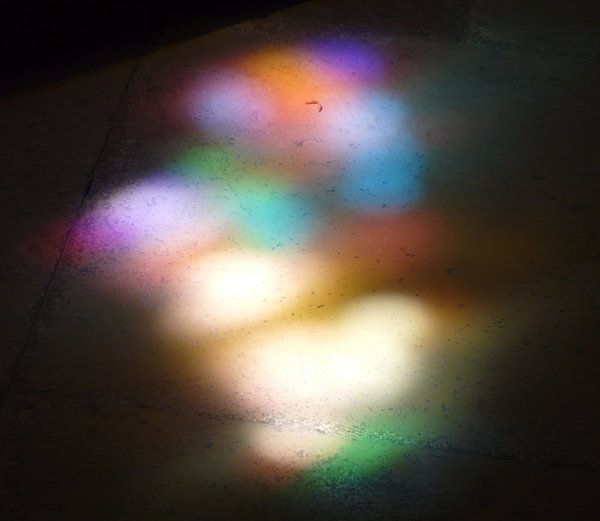
\includegraphics[width=\linewidth]{lichtspiel.jpg}};\end{tcbcliptitle}}]
\lipsum[1]
\end{tcolorbox}
\end{dispExample}
\end{docEnvironment}

\clearpage
\begin{docTcbKey}{clip title}{\colOpt{=true\textbar false}}{default |true|, initially |false|}
  Sets the title to be clipped to the title area.
\begin{dispExample}
\tcbset{enhanced,width=5cm,colframe=red!50!white,coltitle=black,
  colbacktitle=yellow!50!white}

\begin{tcolorbox}[title=\mbox{This is a title which is unbreakable and far too long}]
This is a tcolorbox.
\end{tcolorbox}

\begin{tcolorbox}[title=\mbox{This is a title which is unbreakable and far too long},
  clip title]
This is a tcolorbox.
\end{tcolorbox}
\end{dispExample}
\end{docTcbKey}


\begin{docTcbKey}{clip upper}{\colOpt{=true\textbar false}}{default |true|, initially |false|}
  Sets the upper part to be clipped to the interior area.
\begin{dispExample}
\newcommand{\mygraphics}[2][]{%
  \tcbox[enhanced,boxsep=0pt,top=0pt,bottom=0pt,left=0pt,
    right=0pt,boxrule=0.4pt,drop fuzzy shadow,clip upper,
    colback=black!75!white,toptitle=2pt,bottomtitle=2pt,nobeforeafter,
    center title,fonttitle=\small\sffamily,title=\detokenize{#2}]
  {\includegraphics[width=\the\dimexpr(\linewidth-4mm)/2\relax]{#2}}}

\mygraphics{lichtspiel.jpg}\hfill
\mygraphics{Basilica_5.png}
\end{dispExample}
\end{docTcbKey}

\clearpage
The example for \refKey{/tcb/clip upper} sizes the box according to
the dimensions of the picture. To do it the other way around, the watermark
options provide an easy solution.
\begin{dispExample}
\newcommand{\mygraphics}[2][]{%
  \tcbox[enhanced,capture=minipage,boxsep=0pt,top=0pt,bottom=0pt,left=0pt,
    right=0pt,boxrule=0.4pt,drop fuzzy shadow,nobeforeafter,
    colback=black!75!white,toptitle=2pt,bottomtitle=2pt,
    center title,fonttitle=\small\sffamily,title=\detokenize{#2},
    width=(\linewidth-4mm)/2,height=6cm,colbacktitle={black},
    watermark zoom=1.0,watermark graphics={#2}]{}}

\mygraphics{lichtspiel.jpg}\hfill
\mygraphics{Basilica_5.png}
\end{dispExample}


\begin{docTcbKey}{clip lower}{\colOpt{=true\textbar false}}{default |true|, initially |false|}
  Sets the lower part to be clipped to the interior area.
\begin{dispExample}
\tcbset{enhanced,width=5cm,colframe=red!50!black,text and listing}

\begin{tcblisting}{}
Donau\-dampf\-schiff\-fahrts\-ka\-pi\-t\"ans\-m\"ut\-zen\-fran\-sen
\end{tcblisting}

\begin{tcblisting}{clip lower}
Donau\-dampf\-schiff\-fahrts\-ka\-pi\-t\"ans\-m\"ut\-zen\-fran\-sen
\end{tcblisting}
\end{dispExample}
\end{docTcbKey}


\clearpage
\subsection{Border Line Option Keys}\label{subsec:borderline}
The following borderline options are applicable for most skins which
use |tikzpicture| as \refKey{/tcb/graphical environment}.
Therefore, the skin \refSkin{standard} does not support these border lines,
but most other skins, e.\,g.\ \refSkin{enhanced}.

The borderlines are independent from the normal |tcolorbox| rules.
They may be used with or without the \refKey{/tcb/segmentation engine}.

The borderlines are stackable, i.\,e.\ several different border lines can be
used on the same |tcolorbox|. They are drawn \emph{after} the box frame and box
interior and \emph{before} overlays or watermarks.

\begin{marker}
Technically, the normal |tcolorbox| rules result from a \tikzname\  \emph{filling}
process. The border lines are created by a \tikzname\  \emph{drawing} process.
This can be used to apply different effects.
\end{marker}


\begin{docTcbKey}{borderline}{=\marg{width}\marg{offset}\marg{options}}{no default, initially unset}
  Adds a new borderline to the stack of border lines.
  This border line is drawn with the given \meta{width} and gets an
  \meta{offset} computed from the frame outline. A positive \meta{offset} value
  moves the borderline inside the |tcolorbox| and a negative \meta{offset} value
  moves it outside without changing the bounding box.\\
  The border line is drawn along a \tikzname\  path with the given \tikzname\  \meta{options}.
  Note that the \tikzname\  |line width| option should not be used here.\\
  The border lines adapt to the rounded corners of the |tcolorbox|. An inside
  borderline will switch to sharp corners if necessary, an outside borderline will
  always be rounded except for \refKey{/tcb/sharp corners}.
\begin{dispExample}
\begin{tcolorbox}[enhanced,title=Rounded corners,fonttitle=\bfseries,boxsep=5pt,
  arc=8pt,
  borderline={0.5pt}{0pt}{red},
  borderline={0.5pt}{5pt}{blue,dotted},
  borderline={0.5pt}{-5pt}{green} ]
This is a tcolorbox.
\end{tcolorbox}
\bigskip
\begin{tcolorbox}[enhanced,title=Sharp corners,fonttitle=\bfseries,boxsep=5pt,
  arc=8pt,sharp corners=downhill,
  borderline={0.5pt}{0pt}{red},
  borderline={0.5pt}{5pt}{blue,dotted},
  borderline={0.5pt}{-5pt}{green} ]
This is a tcolorbox.
\end{tcolorbox}
\end{dispExample}

\begin{dispExample}
% \usepackage{lipsum}
\begin{tcolorbox}[enhanced,arc=3mm,boxrule=1.5mm,boxsep=1.5mm,
  colback=yellow!20!white,
  colframe=blue,
  borderline={1mm}{1mm}{white},
  borderline={1mm}{2mm}{red} ]
  \lipsum[1]
\end{tcolorbox}
\end{dispExample}


\begin{dispExample}
% \usepackage{lipsum}
\begin{tcolorbox}[enhanced,arc=3mm,boxrule=1.5mm,
  frame hidden,colback=blue!10!white,
  borderline={1mm}{0mm}{blue,dotted} ]
  \lipsum[2]
\end{tcolorbox}
\end{dispExample}


\begin{dispExample}
% \usepackage{lipsum}
\begin{tcolorbox}[enhanced,skin=enhancedmiddle,
  frame hidden,interior hidden,top=0mm,bottom=0mm,boxsep=0mm,
  borderline={0.75mm}{0mm}{red},
  borderline={0.75mm}{0.75mm}{red!50!yellow},
  borderline={0.75mm}{1.5mm}{yellow}, ]
  \lipsum[3]
\end{tcolorbox}
\end{dispExample}

\begin{dispExample}
% \usepackage{lipsum}
\newtcolorbox{mygreenbox}[2][]{%
  enhanced,width=\linewidth-6pt,
  enlarge top by=3pt,enlarge bottom by=3pt,
  enlarge left by=3pt,enlarge right by=3pt,
  title={#2},frame hidden,boxrule=0pt,top=1mm,bottom=1mm,
  colframe=green!30!black, colbacktitle=green!50!yellow,
  coltitle=black, colback=green!25!white,
  borderline={0.5pt}{-0.5pt}{green!75!blue},
  borderline={1pt}{-3pt}{green!50!blue},#1}

\begin{mygreenbox}{My title}
  \lipsum[4]
\end{mygreenbox}
\end{dispExample}
\end{docTcbKey}


\begin{docTcbKey}{no borderline}{}{no default, initially set}
  Removes all borderlines if set before.
\end{docTcbKey}


\begin{docTcbKey}{show bounding box}{\colOpt{=\meta{color}}}{default |red|, initially unset}
  Displays the bounding box borderline of a |tcolorbox|.
  Its intended use is debugging and fine tuning.
  It should not be part of a final document.
  The optional \meta{color} is the base color for the bounding box
  borderline.
\begin{dispExample}
\tcbset{enhanced,nobeforeafter,width=4cm,fonttitle=\bfseries}

\begin{tcolorbox}[show bounding box,title=Normal]
This is a tcolorbox.
\end{tcolorbox}%
\begin{tcolorbox}[show bounding box=blue,title=Shadow,drop fuzzy shadow]
This is a tcolorbox.
\end{tcolorbox}%
\begin{tcolorbox}[show bounding box=green,title=Enlarged,drop fuzzy shadow,
  enlarge by=2mm]
This is a tcolorbox.
\end{tcolorbox}
\end{dispExample}
\end{docTcbKey}

\clearpage

\begin{marker}
The following \emph{partial} borderlines act slightly different from the
complete borderlines described before. They ignore rounded corner settings,
their length is not modified by their \meta{offset}, they ignore skin settings
but adapt to breakable boxes.
\end{marker}

\begin{docTcbKey}[][doc new=2014-10-20]{borderline north}{=\marg{width}\marg{offset}\marg{options}}{no default, initially unset}
  Adds a new borderline with the given \meta{width} to the
  north of the |tcolorbox|.
  A positive \meta{offset} value
  moves the borderline inside the |tcolorbox| and a negative \meta{offset} value
  moves it outside without changing the bounding box.
\begin{dispExample*}{sbs,lefthand ratio=0.6}
\begin{tcolorbox}[enhanced,
  borderline north={2pt}{-2pt}{red}]
  This is a \textbf{tcolorbox}.
\end{tcolorbox}
\end{dispExample*}
\end{docTcbKey}

\begin{docTcbKey}[][doc new=2014-10-20]{borderline south}{=\marg{width}\marg{offset}\marg{options}}{no default, initially unset}
  Adds a new borderline with the given \meta{width} to the
  south of the |tcolorbox|.
  A positive \meta{offset} value
  moves the borderline inside the |tcolorbox| and a negative \meta{offset} value
  moves it outside without changing the bounding box.
\begin{dispExample*}{sbs,lefthand ratio=0.6}
\begin{tcolorbox}[enhanced,
  borderline south={2pt}{-2pt}{red}]
  This is a \textbf{tcolorbox}.
\end{tcolorbox}
\end{dispExample*}
\end{docTcbKey}

\begin{docTcbKey}[][doc new=2014-10-20]{borderline east}{=\marg{width}\marg{offset}\marg{options}}{no default, initially unset}
  Adds a new borderline with the given \meta{width} to the
  east of the |tcolorbox|.
  A positive \meta{offset} value
  moves the borderline inside the |tcolorbox| and a negative \meta{offset} value
  moves it outside without changing the bounding box.
\begin{dispExample*}{sbs,lefthand ratio=0.6}
\begin{tcolorbox}[enhanced,
  borderline east={2pt}{-2pt}{red}]
  This is a \textbf{tcolorbox}.
\end{tcolorbox}
\end{dispExample*}
\end{docTcbKey}

\begin{docTcbKey}[][doc new=2014-10-20]{borderline west}{=\marg{width}\marg{offset}\marg{options}}{no default, initially unset}
  Adds a new borderline with the given \meta{width} to the
  west of the |tcolorbox|.
  A positive \meta{offset} value
  moves the borderline inside the |tcolorbox| and a negative \meta{offset} value
  moves it outside without changing the bounding box.
\begin{dispExample*}{sbs,lefthand ratio=0.6}
\begin{tcolorbox}[enhanced,
  borderline west={2pt}{-2pt}{red}]
  This is a \textbf{tcolorbox}.
\end{tcolorbox}
\end{dispExample*}
\end{docTcbKey}

\clearpage
\begin{docTcbKey}[][doc new=2014-10-20]{borderline horizontal}{=\marg{width}\marg{offset}\marg{options}}{no default, initially unset}
  Adds a new borderline with the given \meta{width} to the
  north and south of the |tcolorbox|.
  A positive \meta{offset} value
  moves the borderlines inside the |tcolorbox| and a negative \meta{offset} value
  moves them outside without changing the bounding box.
\begin{dispExample*}{sbs,lefthand ratio=0.6}
\begin{tcolorbox}[blanker,top=3mm,bottom=3mm,
   borderline horizontal={2pt}{0pt}{red}]
  This is a \textbf{tcolorbox}.
\end{tcolorbox}
\end{dispExample*}
\end{docTcbKey}


\begin{docTcbKey}[][doc new=2014-10-20]{borderline vertical}{=\marg{width}\marg{offset}\marg{options}}{no default, initially unset}
  Adds a new borderline with the given \meta{width} to the
  east and west of the |tcolorbox|.
  A positive \meta{offset} value
  moves the borderlines inside the |tcolorbox| and a negative \meta{offset} value
  moves them outside without changing the bounding box.
\begin{dispExample*}{sbs,lefthand ratio=0.6}
\begin{tcolorbox}[blanker,left=3mm,right=3mm,
   borderline vertical={2pt}{0pt}{red}]
  This is a \textbf{tcolorbox}.\\
  My second line.
\end{tcolorbox}
\end{dispExample*}
\end{docTcbKey}

\begin{dispExample}
\begin{tcolorbox}[enhanced,colback=yellow!10!white,boxrule=0pt,frame hidden,
  borderline north={1mm}{-2mm}{red},
  borderline south={1mm}{-2mm}{blue},
  borderline west={1mm}{-2mm}{green},
  borderline east={1mm}{-2mm}{yellow}]
\lipsum[1]
\end{tcolorbox}
\end{dispExample}

\clearpage
\subsection{Shadow Option Keys}\label{subsec:shadows}
The following shadow options are applicable for most skins which
use |tikzpicture| as \refKey{/tcb/graphical environment}.
Therefore, the skin \refSkin{standard} does not support these shadows,
but most other skins, e.\,g.\ \refSkin{enhanced}.

The shadows are stackable, i.\,e.\ several different shadows can be
used on the same |tcolorbox|. They are drawn \emph{before} the box frame is drawn.

\begin{docTcbKey}{no shadow}{}{no default}
  Removes all shadows if set before.
\end{docTcbKey}

\subsubsection{Common Shadows and Halos}

\begin{docTcbKey}{drop shadow}{\colOpt{=\meta{color}}}{style, default |black!50!white|}
  Adds a new shadow with standard dimensions to the stack of shadows.
  Optionally, the \meta{color} for the shadow can be changed.
\begin{dispExample*}{sbs,lefthand ratio=0.6}
\tcbset{enhanced,colback=red!5!white,
  colframe=red!75!black,fonttitle=\bfseries}

\begin{tcolorbox}[drop shadow]
This is a tcolorbox.
\end{tcolorbox}\par\bigskip
\begin{tcolorbox}[title=Another shadow,
  drop shadow=blue]
This is a tcolorbox.
\end{tcolorbox}
\end{dispExample*}
\end{docTcbKey}


\begin{docTcbKey}{drop fuzzy shadow}{\colOpt{=\meta{color}}}{style, default |black!50!white|}
  Adds a new fuzzy shadow with standard dimensions to the stack of shadows.
  Optionally, the \meta{color} for the shadow can be changed.
\begin{dispExample*}{sbs,lefthand ratio=0.6}
\tcbset{enhanced,colback=red!5!white,
  colframe=red!75!black,fonttitle=\bfseries}

\begin{tcolorbox}[drop fuzzy shadow]
This is a tcolorbox.
\end{tcolorbox}\par\bigskip
\begin{tcolorbox}[title=Another shadow,
  drop fuzzy shadow=blue]
This is a tcolorbox.
\end{tcolorbox}
\end{dispExample*}
\end{docTcbKey}


\begin{docTcbKey}{drop midday shadow}{\colOpt{=\meta{color}}}{style, default |black!50!white|}
  Adds a new shadow with standard dimensions to the stack of shadows.
  Optionally, the \meta{color} for the shadow can be changed.
\begin{dispExample*}{sbs,lefthand ratio=0.6}
\tcbset{enhanced,colback=red!5!white,
  colframe=red!75!black,fonttitle=\bfseries}

\begin{tcolorbox}[drop midday shadow]
This is a tcolorbox.
\end{tcolorbox}\par\bigskip
\begin{tcolorbox}[title=Another shadow,
  drop midday shadow=blue]
This is a tcolorbox.
\end{tcolorbox}
\end{dispExample*}
\end{docTcbKey}

%\enlargethispage*{2cm}
\begin{docTcbKey}{drop fuzzy midday shadow}{\colOpt{=\meta{color}}}{style, default |black!50!white|}
  Adds a new fuzzy shadow with standard dimensions to the stack of shadows.
  Optionally, the \meta{color} for the shadow can be changed.
\begin{dispExample*}{sbs,lefthand ratio=0.6}
\tcbset{enhanced,colback=red!5!white,
  colframe=red!75!black,fonttitle=\bfseries}

\begin{tcolorbox}[drop fuzzy midday shadow]
This is a tcolorbox.
\end{tcolorbox}\par\bigskip
\begin{tcolorbox}[title=Another shadow,
  drop fuzzy midday shadow=blue]
This is a tcolorbox.
\end{tcolorbox}
\end{dispExample*}
\end{docTcbKey}


\begin{docTcbKey}{halo}{\colOpt{=\meta{size} \texttt{with} \meta{color}}}{style, default |0.9mm with yellow|}
  Adds a new halo shadow with the given \meta{color}
  which overlaps the colorbox an all sides by \meta{size}.
\begin{dispExample*}{sbs,lefthand ratio=0.6}
\tcbset{enhanced,colback=red!5!white,
  colframe=red!75!black,fonttitle=\bfseries}

\begin{tcolorbox}[title=My own halo,halo]
This is a tcolorbox.
\end{tcolorbox}
\par\bigskip\bigskip
\begin{tcolorbox}[title=Another halo,
  halo=2mm with green]
This is a tcolorbox.
\end{tcolorbox}
\end{dispExample*}
\end{docTcbKey}

\enlargethispage*{2cm}
\begin{docTcbKey}{fuzzy halo}{\colOpt{=\meta{size} \texttt{with} \meta{color}}}{style, default |0.9mm with yellow|}
  Adds a new fuzzy halo shadow with the given \meta{color}
  which overlaps the colorbox an all sides by \meta{size} plus |0.48mm|.
\begin{dispExample*}{sbs,lefthand ratio=0.6}
\tcbset{enhanced,colback=red!5!white,
  colframe=red!75!black,fonttitle=\bfseries}

\begin{tcolorbox}[title=My own halo,fuzzy halo]
This is a tcolorbox.
\end{tcolorbox}
\par\bigskip\bigskip
\begin{tcolorbox}[title=Another halo,
  fuzzy halo=2mm with green]
This is a tcolorbox.
\end{tcolorbox}
\end{dispExample*}

\begin{dispExample}
\begin{tcolorbox}[blank,enhanced jigsaw,boxsep=2pt,arc=2pt,
  fuzzy halo=2mm with red!50!white,
  fuzzy halo=1mm with white]
\lipsum[1]
\end{tcolorbox}
\end{dispExample}
\end{docTcbKey}


\clearpage
For all following shadows, the optionally given \meta{color} for the shadow can be changed
equivalent to the preceding examples.

\begin{docTcbKey}{drop shadow southeast}{\colOpt{=\meta{color}}}{style, default |black!50!white|}
  Adds a new shadow with standard dimensions to the stack of shadows.
  This shadow is identical to \refKey{/tcb/drop shadow}.
\begin{dispExample*}{sbs,lefthand ratio=0.7}
\begin{tcolorbox}[drop shadow southeast,
  enhanced,colback=red!5!white,colframe=red!75!black]
  This is a tcolorbox.
\end{tcolorbox}
\end{dispExample*}
\end{docTcbKey}%

\begin{docTcbKey}{drop shadow south}{\colOpt{=\meta{color}}}{style, default |black!50!white|}
  Adds a new shadow with standard dimensions to the stack of shadows.
  This shadow is identical to \refKey{/tcb/drop midday shadow}.
\begin{dispExample*}{sbs,lefthand ratio=0.7}
\begin{tcolorbox}[drop shadow south,
  enhanced,colback=red!5!white,colframe=red!75!black]
  This is a tcolorbox.
\end{tcolorbox}
\end{dispExample*}
\end{docTcbKey}%

\begin{docTcbKey}{drop shadow southwest}{\colOpt{=\meta{color}}}{style, default |black!50!white|}
  Adds a new shadow with standard dimensions to the stack of shadows.
\begin{dispExample*}{sbs,lefthand ratio=0.7}
\begin{tcolorbox}[drop shadow southwest,
  enhanced,colback=red!5!white,colframe=red!75!black]
  This is a tcolorbox.
\end{tcolorbox}
\end{dispExample*}
\end{docTcbKey}%

\begin{docTcbKey}{drop shadow west}{\colOpt{=\meta{color}}}{style, default |black!50!white|}
  Adds a new shadow with standard dimensions to the stack of shadows.
\begin{dispExample*}{sbs,lefthand ratio=0.7}
\begin{tcolorbox}[drop shadow west,
  enhanced,colback=red!5!white,colframe=red!75!black]
  This is a tcolorbox.
\end{tcolorbox}
\end{dispExample*}
\end{docTcbKey}%

\begin{docTcbKey}{drop shadow northwest}{\colOpt{=\meta{color}}}{style, default |black!50!white|}
  Adds a new shadow with standard dimensions to the stack of shadows.
\begin{dispExample*}{sbs,lefthand ratio=0.7}
\begin{tcolorbox}[drop shadow northwest,
  enhanced,colback=red!5!white,colframe=red!75!black]
  This is a tcolorbox.
\end{tcolorbox}
\end{dispExample*}
\end{docTcbKey}%

\begin{docTcbKey}{drop shadow north}{\colOpt{=\meta{color}}}{style, default |black!50!white|}
  Adds a new shadow with standard dimensions to the stack of shadows.
\begin{dispExample*}{sbs,lefthand ratio=0.7}
\begin{tcolorbox}[drop shadow north,
  enhanced,colback=red!5!white,colframe=red!75!black]
  This is a tcolorbox.
\end{tcolorbox}
\end{dispExample*}
\end{docTcbKey}%

\clearpage
\begin{docTcbKey}{drop shadow northeast}{\colOpt{=\meta{color}}}{style, default |black!50!white|}
  Adds a new shadow with standard dimensions to the stack of shadows.
\begin{dispExample*}{sbs,lefthand ratio=0.7}
\begin{tcolorbox}[drop shadow northeast,
  enhanced,colback=red!5!white,colframe=red!75!black]
  This is a tcolorbox.
\end{tcolorbox}
\end{dispExample*}
\end{docTcbKey}%

\begin{docTcbKey}{drop shadow east}{\colOpt{=\meta{color}}}{style, default |black!50!white|}
  Adds a new shadow with standard dimensions to the stack of shadows.
\begin{dispExample*}{sbs,lefthand ratio=0.7}
\begin{tcolorbox}[drop shadow east,
  enhanced,colback=red!5!white,colframe=red!75!black]
  This is a tcolorbox.
\end{tcolorbox}
\end{dispExample*}
\end{docTcbKey}%


\begin{docTcbKey}{drop fuzzy shadow southeast}{\colOpt{=\meta{color}}}{style, default |black!50!white|}
  Adds a new fuzzy shadow with standard dimensions to the stack of shadows.
  This shadow is identical to \refKey{/tcb/drop fuzzy shadow}.
\begin{dispExample*}{sbs,lefthand ratio=0.7}
\begin{tcolorbox}[drop fuzzy shadow southeast,
  enhanced,colback=red!5!white,colframe=red!75!black]
  This is a tcolorbox.
\end{tcolorbox}
\end{dispExample*}
\end{docTcbKey}%

\begin{docTcbKey}{drop fuzzy shadow south}{\colOpt{=\meta{color}}}{style, default |black!50!white|}
  Adds a new fuzzy shadow with standard dimensions to the stack of shadows.
  This shadow is identical to \refKey{/tcb/drop fuzzy midday shadow}.
\begin{dispExample*}{sbs,lefthand ratio=0.7}
\begin{tcolorbox}[drop fuzzy shadow south,
  enhanced,colback=red!5!white,colframe=red!75!black]
  This is a tcolorbox.
\end{tcolorbox}
\end{dispExample*}
\end{docTcbKey}%

\begin{docTcbKey}{drop fuzzy shadow southwest}{\colOpt{=\meta{color}}}{style, default |black!50!white|}
  Adds a new fuzzy shadow with standard dimensions to the stack of shadows.
\begin{dispExample*}{sbs,lefthand ratio=0.7}
\begin{tcolorbox}[drop fuzzy shadow southwest,
  enhanced,colback=red!5!white,colframe=red!75!black]
  This is a tcolorbox.
\end{tcolorbox}
\end{dispExample*}
\end{docTcbKey}%

\begin{docTcbKey}{drop fuzzy shadow west}{\colOpt{=\meta{color}}}{style, default |black!50!white|}
  Adds a new fuzzy shadow with standard dimensions to the stack of shadows.
\begin{dispExample*}{sbs,lefthand ratio=0.7}
\begin{tcolorbox}[drop fuzzy shadow west,
  enhanced,colback=red!5!white,colframe=red!75!black]
  This is a tcolorbox.
\end{tcolorbox}
\end{dispExample*}
\end{docTcbKey}%

\clearpage
\begin{docTcbKey}{drop fuzzy shadow northwest}{\colOpt{=\meta{color}}}{style, default |black!50!white|}
  Adds a new fuzzy shadow with standard dimensions to the stack of shadows.
\begin{dispExample*}{sbs,lefthand ratio=0.7}
\begin{tcolorbox}[drop fuzzy shadow northwest,
  enhanced,colback=red!5!white,colframe=red!75!black]
  This is a tcolorbox.
\end{tcolorbox}
\end{dispExample*}
\end{docTcbKey}%

\begin{docTcbKey}{drop fuzzy shadow north}{\colOpt{=\meta{color}}}{style, default |black!50!white|}
  Adds a new fuzzy shadow with standard dimensions to the stack of shadows.
\begin{dispExample*}{sbs,lefthand ratio=0.7}
\begin{tcolorbox}[drop fuzzy shadow north,
  enhanced,colback=red!5!white,colframe=red!75!black]
  This is a tcolorbox.
\end{tcolorbox}
\end{dispExample*}
\end{docTcbKey}%

\begin{docTcbKey}{drop fuzzy shadow northeast}{\colOpt{=\meta{color}}}{style, default |black!50!white|}
  Adds a new fuzzy shadow with standard dimensions to the stack of shadows.
\begin{dispExample*}{sbs,lefthand ratio=0.7}
\begin{tcolorbox}[drop fuzzy shadow northeast,
  enhanced,colback=red!5!white,colframe=red!75!black]
  This is a tcolorbox.
\end{tcolorbox}
\end{dispExample*}
\end{docTcbKey}%

\begin{docTcbKey}{drop fuzzy shadow east}{\colOpt{=\meta{color}}}{style, default |black!50!white|}
  Adds a new fuzzy shadow with standard dimensions to the stack of shadows.
\begin{dispExample*}{sbs,lefthand ratio=0.7}
\begin{tcolorbox}[drop fuzzy shadow east,
  enhanced,colback=red!5!white,colframe=red!75!black]
  This is a tcolorbox.
\end{tcolorbox}
\end{dispExample*}
\end{docTcbKey}%


\clearpage
\subsubsection{Lifted Shadows}

\begin{docTcbKey}{drop lifted shadow}{\colOpt{=\meta{color}}}{style, default |black!50!white|}
  Adds a new lifted shadow with standard dimensions to the stack of shadows.
  Optionally, the \meta{color} for the shadow can be changed.
\begin{dispExample*}{sbs,lefthand ratio=0.6}
\tcbset{enhanced,colback=red!5!white,
  boxrule=0.4pt,sharp corners,
  colframe=red!75!black,fonttitle=\bfseries}

\begin{tcolorbox}[drop lifted shadow]
This is a tcolorbox.
\end{tcolorbox}\par\bigskip
\begin{tcolorbox}[title=Another shadow,
  drop lifted shadow=blue]
This is a tcolorbox.
\end{tcolorbox}
\end{dispExample*}
\end{docTcbKey}


\begin{docTcbKey}{drop small lifted shadow}{\colOpt{=\meta{color}}}{style, default |black!50!white|}
  Adds a new small lifted shadow with standard dimensions to the stack of shadows.
  Optionally, the \meta{color} for the shadow can be changed.
\begin{dispExample*}{sbs,lefthand ratio=0.6}
\tcbset{enhanced,colback=red!5!white,
  boxrule=0.4pt,sharp corners,
  colframe=red!75!black,fonttitle=\bfseries}

\tcbox[drop small lifted shadow,size=fbox]
  {This is a tcolorbox.}
\par\bigskip
\begin{tcolorbox}[title=Another shadow,
  drop small lifted shadow=black]
This is a tcolorbox.
\end{tcolorbox}
\end{dispExample*}
\end{docTcbKey}


\begin{docTcbKey}{drop large lifted shadow}{\colOpt{=\meta{color}}}{style, default |black!50!white|}
  Adds a new large lifted shadow with standard dimensions to the stack of shadows.
  Optionally, the \meta{color} for the shadow can be changed.
\begin{dispExample*}{sbs,lefthand ratio=0.6}
\tcbset{enhanced,colback=red!5!white,
  colframe=red!75!black,fonttitle=\bfseries}

\begin{tcolorbox}[drop large lifted shadow]
This is a tcolorbox.
\end{tcolorbox}\par\bigskip
\begin{tcolorbox}[title=Another shadow,
  drop large lifted shadow=blue]
This is a tcolorbox.
\end{tcolorbox}
\end{dispExample*}
\end{docTcbKey}


\clearpage

\subsubsection{Generic Shadows}
\begin{docTcbKey}{shadow}{=\marg{xshift}\marg{yshift}\marg{offset}\marg{options}}{no default}
  Adds a new shadow to the stack of shadows.
  This shadow follows the outline of the |tcolorbox| but is shifted by
  \meta{xshift} and \meta{yshift}. The \meta{offset} value is a distance value
  from the frame outline.  A positive \meta{offset} value shrinks the shadow
  and a negative \meta{offset} value enlarges the shadow.
  The shadow is filled along a \tikzname\  path with the given \tikzname\  \meta{options}.\\
  The shadows adapt to the rounded corners of the |tcolorbox|. An shrinked shadow
  will switch to sharp corners if necessary, an enlarged shadow may become
  more rounded depending on several factors. But \refKey{/tcb/sharp corners}
  have sharp shadows.
  \begin{marker}
  Shadows are not considered for the bounding box computation by default.
  Large shadows may be overlaped by the following content. But, the
  bounding box can be adapted if necessary.
  \end{marker}

\begin{dispExample*}{sbs,lefthand ratio=0.6}
\tcbset{enhanced,colback=red!5!white,
  colframe=red!75!black,fonttitle=\bfseries}

\begin{tcolorbox}[title=My own shadow,
  shadow={2mm}{-1mm}{0mm}{black!50!white}]
This is a tcolorbox.
\end{tcolorbox}
\par\bigskip
\begin{tcolorbox}[title=Another shadow,
  shadow={-1mm}{-2mm}{0mm}{fill=blue,
    opacity=0.5}]
This is a tcolorbox.
\end{tcolorbox}
\par\bigskip
\begin{tcolorbox}[title=Double shadow,
  shadow={-1.5mm}{-1.5mm}{0mm}{fill=blue,
    opacity=0.25},
  shadow={1.5mm}{-1.5mm}{0mm}{fill=red,
    opacity=0.25}]
This is a tcolorbox.
\end{tcolorbox}
\par\bigskip
\begin{tcolorbox}[title=Far shadow,
  shadow={5.5mm}{-3.5mm}{2mm}{fill=black,
    opacity=0.25}]
This is a tcolorbox.
\end{tcolorbox}
\par\bigskip\bigskip
\begin{tcolorbox}[title=Halo shadow,
  shadow={0mm}{0mm}{-1.5mm}%
     {fill=yellow!75!red,opacity=0.5}]
This is a tcolorbox.
\end{tcolorbox}
\end{dispExample*}
\end{docTcbKey}

\clearpage
\begin{docTcbKey}{fuzzy shadow}{=\marg{xshift}\marg{yshift}\marg{offset}\marg{step}\marg{options}}{no default}
  Adds a new fuzzy shadow to the stack of shadows. Actually, this option
  adds several shadows which appear like a shadow with a fuzzy border.
  This fuzzy shadow follows the outline of the |tcolorbox| but is shifted by
  \meta{xshift} and \meta{yshift}. The \meta{offset} value is a distance value
  from the frame outline.  A positive \meta{offset} value shrinks the shadow
  and a negative \meta{offset} value enlarges the shadow.
  The \marg{step} value describes a shrink
  offset used for the combination of the partial shadows.
  The shadow is filled along a \tikzname\  path with the given \tikzname\  \meta{options} but
  any |opacity| value will be ignored.
\begin{dispExample*}{sbs,lefthand ratio=0.6}
\tcbset{enhanced,colback=red!5!white,
  colframe=red!75!black,fonttitle=\bfseries}

\begin{tcolorbox}[title=My own shadow,
  fuzzy shadow={2mm}{-1mm}{0mm}{0.1mm}%
               {black!50!white}]
This is a tcolorbox.
\end{tcolorbox}
\par\bigskip
\begin{tcolorbox}[title=Another shadow,
  fuzzy shadow={-1mm}{-2mm}{0mm}{0.2mm}%
               {fill=blue}]
This is a tcolorbox.
\end{tcolorbox}
\par\bigskip
\begin{tcolorbox}[title=Double shadow,
  fuzzy shadow={-1.5mm}{-1.5mm}{0mm}{0.1mm}%
               {blue},
  fuzzy shadow={1.5mm}{-1.5mm}{0mm}{0.1mm}%
               {red}]
This is a tcolorbox.
\end{tcolorbox}
\par\bigskip
\begin{tcolorbox}[title=Far shadow,
  fuzzy shadow={5.5mm}{-3.5mm}{0mm}{0.3mm}%
               {black}]
This is a tcolorbox.
\end{tcolorbox}
\par\bigskip\bigskip
\begin{tcolorbox}[title=Glow shadow,
  fuzzy shadow={0mm}{0mm}{-1.5mm}{0.15mm}%
               {yellow!75!red}]
This is a tcolorbox.
\end{tcolorbox}
\end{dispExample*}

\begin{dispExample}
\newtcolorbox{mybox}[1][]{enhanced,
  fuzzy shadow={1.0mm}{-1.0mm}{0.12mm}{0mm}{blue!50!white},
  fuzzy shadow={-1.0mm}{-1.0mm}{0.12mm}{0mm}{red!50!white},
  fuzzy shadow={-1.0mm}{1.0mm}{0.12mm}{0mm}{green!50!white},
  fuzzy shadow={1.0mm}{1.0mm}{0.12mm}{0mm}{yellow!50!white},#1
}

\begin{mybox}[title=A multi shadow box]
This is a tcolorbox.
\end{mybox}
\end{dispExample}
\end{docTcbKey}


\clearpage
\begin{docTcbKey}[][doc new=2015-05-05]{smart shadow arc}{\colOpt{=true\textbar false}}{default |true|,
  initially |true|}
If set to |true|, the shadow drawing algorithm tries to do a somewhat
smart calculation of the arc for the shadow. The result is pleasing for typical boxes
with rounded corners, but gives strange results for circular boxes.

\begin{dispExample}
\tcbset{enhanced,nobeforeafter,colback=red!5!white,
  colframe=red!75!black,width=3cm,square,halign=center,valign=center
  }

\begin{tcolorbox}[drop shadow]
Smart shadow arc (arguably better than normal)
\end{tcolorbox}
\hfill
\begin{tcolorbox}[smart shadow arc=false, drop shadow]
Normal shadow arc
\end{tcolorbox}
\hfill
\begin{tcolorbox}[circular arc, drop shadow]
Smart shadow arc (worse than normal)
\end{tcolorbox}
\hfill
\begin{tcolorbox}[circular arc, smart shadow arc=false, drop shadow]
Normal shadow arc
\end{tcolorbox}
\end{dispExample}
\end{docTcbKey}


\begin{docTcbKey}{lifted shadow}{=\marg{xshift}\marg{yshift}\marg{bend}\marg{step}\marg{options}}{no default}
  Adds a new lifted shadow to the stack of shadows. Actually, this option
  adds several shadows which appear like a shadow with a fuzzy border.
  This lifted shadow follows the outline of the |tcolorbox| but is shifted by
  \meta{xshift} and \meta{yshift} on the lower left corner and by
  $-$\meta{xshift} and \meta{yshift} on the lower right corner.
  Additionally, there is a \meta{bend} in the middle.
  The \marg{step} value describes a shrink
  offset used for the combination of the partial shadows.
  The shadow is filled along a \tikzname\  path with the given \tikzname\  \meta{options} but
  any |opacity| value will be ignored.
\begin{dispExample*}{sbs,lefthand ratio=0.6}
\tcbset{enhanced,colback=red!5!white,
  boxrule=0.1pt,
  colframe=red!75!black,fonttitle=\bfseries}

\begin{tcolorbox}[title=My own shadow,
  lifted shadow={1mm}{-2mm}{3mm}{0.1mm}%
               {black!50!white}]
This is a tcolorbox.
\end{tcolorbox}
\end{dispExample*}
\end{docTcbKey}

\clearpage
\subsubsection{\tikzname\ Shadows}
Alternativ to the package shadow options described before, shadows from
the \flqq Shadows Library\frqq\ of \tikzname\ can be used.
Such shadows can be added directly to the frame path using \refKey{/tcb/frame style}.

\begin{exdispExample*}{tikz_shadow_1}{sbs,lefthand ratio=0.7}
% \usetikzlibrary{shadows}
\begin{tcolorbox}[enhanced,
  colback=red!5!white,colframe=red!75!black,
  frame style={drop shadow} ]
  This is a tcolorbox.
\end{tcolorbox}
\end{exdispExample*}

\begin{exdispExample*}{tikz_shadow_2}{sbs,lefthand ratio=0.7}
% \usetikzlibrary{shadows}
\begin{tcolorbox}[enhanced,height=3cm,
  colback=red!5!white,colframe=red!75!black,
  halign=center,valign=center,
  frame style={circular drop shadow} ]
  This is a tcolorbox.
\end{tcolorbox}
\end{exdispExample*}

\begin{exdispExample*}{tikz_shadow_3}{sbs,lefthand ratio=0.7}
% \usetikzlibrary{shadows}
\begin{tcolorbox}[enhanced,width=2.5cm,
  square,circular arc,
  halign=center,valign=center,
  colback=red!5!white,colframe=red!75!black,
  frame style={circular glow={fill=red}} ]
  tcolorbox
\end{tcolorbox}
\end{exdispExample*}


\clearpage
\subsection{\tikzname\  Picture Option Keys}\label{subsec:tikzpicture}
The following general options are applicable for skins which
use |tikzpicture| as \refKey{/tcb/graphical environment}.
Therefore, the skin \refSkin{standard} does not support these options,
but most other skins, e.\,g.\ \refSkin{enhanced}.


\begin{docTcbKey}{tikz}{=\meta{tikz option list}}{no default, initially empty}
  Adds the given \meta{tikz option list} to the main |tikzpicture| environment
  used to draw the color box, see \cite{tantau:2015a}. If this option is
  applied a second time, the new \meta{tikz option list} is appended to the
  current option list.
\begin{dispExample*}{sbs,lefthand ratio=0.66,
  segmentation style={pattern=checkerboard light gray}}
\tcbset{enhanced,colback=red!5!white,
  colframe=red!75!black,fonttitle=\bfseries}

\begin{tcolorbox}[title=Transparent box,
  tikz={opacity=0.5,transparency group}]
This is a tcolorbox.
\end{tcolorbox}
\end{dispExample*}

\begin{dispExample*}{sbs,lefthand ratio=0.66}
\tcbset{enhanced,colback=red!5!white,
  colframe=red!75!black,fonttitle=\bfseries,
  fontupper=\bfseries\Huge,
  halign title=center,halign=center}

\begin{tcolorbox}[title=Rotated box,
  tikz={rotate=30}]
Sold!
\end{tcolorbox}
\end{dispExample*}

\end{docTcbKey}


\begin{docTcbKey}{tikz reset}{}{initially set}
  Removes all options given by \refKey{/tcb/tikz}.
\end{docTcbKey}


\begin{docTcbKey}{at begin tikz}{=\meta{tikz code}}{no default, initially empty}
  The given \meta{tikz code} is executed at the beginning of the |tikzpicture| environment
  after the \tikzname\  option |execute at begin picture| was applied.
  If this option is applied a second time, the new \meta{tikz code} is appended to the current code.
\end{docTcbKey}


\begin{docTcbKey}{at begin tikz reset}{}{initially set}
  Removes all code given by \refKey{/tcb/at begin tikz}.
\end{docTcbKey}


\begin{docTcbKey}{at end tikz}{=\meta{tikz code}}{no default, initially empty}
  The given \meta{tikz code} is executed at the ending of the |tikzpicture| environment
  before the \tikzname\  option |execute at end picture| was applied.
  If this option is applied a second time, the new \meta{tikz code} is appended to the current code.
\end{docTcbKey}


\begin{docTcbKey}{at end tikz reset}{}{initially set}
  Removes all code given by \refKey{/tcb/at end tikz}.
\end{docTcbKey}


\clearpage
\begin{docTcbKey}{rotate}{=\meta{angle}}{no default, initially unset}
  Rotates the |tcolorbox| by the given \meta{angle}. Note that this is
  a \tikzname\  coordinate transformation i.e. not all graphical elements like shadings
  will really be rotated.
\begin{dispExample*}{sbs,lefthand ratio=0.66}
\tcbset{enhanced,colback=red!5!white,
  colframe=red!75!black,fonttitle=\bfseries}

\begin{tcolorbox}[title=Rotated box,rotate=30]
This is a tcolorbox.
\end{tcolorbox}
\end{dispExample*}
\end{docTcbKey}

\begin{docTcbKey}{scale}{=\meta{fraction}}{no default, initially unset}
  Scales the |tcolorbox| by the given \meta{fraction}. Note that this is
  a \tikzname\  coordinate transformation i.e. not all graphical elements like line widths
  will really be scaled.
\begin{dispExample*}{sbs,lefthand ratio=0.66}
\tcbset{enhanced,colback=red!5!white,
  colframe=red!75!black,fonttitle=\bfseries}

\begin{tcolorbox}[title=Scaled box,scale=0.5]
This is a tcolorbox.
\end{tcolorbox}
\begin{tcolorbox}[title=Scaled box,scale=1.25]
This is a tcolorbox.
\end{tcolorbox}
\end{dispExample*}
\end{docTcbKey}


\begin{docTcbKey}{remember}{}{style, initially unset}
  Shortcut for |tikz={remember picture}|. This allows one to reference nodes
  in other \tikzname\  pictures.
\begin{dispExample}
\begin{tcolorbox}[enhanced,remember,colback=red!5!white,colframe=red!75!black,
  fonttitle=\bfseries,title=The four corners of a paper,
  overlay={\draw[red!50!white,line width=1mm,opacity=0.5,shorten >=3mm]
    (frame.north west) edge[->] (current page.north west)
    (frame.north east) edge[->] (current page.north east)
    (frame.south west) edge[->] (current page.south west)
    (frame.south east) edge[->] (current page.south east);}]
This is a tcolorbox.
\end{tcolorbox}
\end{dispExample}
\end{docTcbKey}

\clearpage
\tcbinterruptdraftmode%
\begin{docTcbKey}{remember as}{=\meta{name}}{style, no default, initially unset}
  The |frame| node will be remembered by the given \meta{name} to be referenced
  in other \tikzname\  pictures.
\begin{dispExample}
% \usepackage{lipsum}
\newtcolorbox{mybox}[1][]{enhanced,colframe=blue!75!black,colback=blue!10!white,
  fonttitle=\bfseries,#1}

\begin{mybox}[title=First Box,nobeforeafter,width=\linewidth/4,remember as=one]
This is a test.
\end{mybox}
\hfill
\begin{mybox}[title=Second Box,nobeforeafter,width=\linewidth/4,remember as=two]
This is a test.
\end{mybox}
\hfill
\begin{mybox}[title=Third Box,nobeforeafter,width=\linewidth/4,remember as=three]
This is a test.
\end{mybox}

\lipsum[2]

\begin{mybox}[title=Fourth Box,remember as=four]
This is a test.
\end{mybox}

\begin{tikzpicture}[overlay,remember picture,line width=1mm,draw=red!75!black]
  \draw[->] (one.east) to[bend right] node[above] {A} (two.west);
  \draw[->] (two.east) to[bend left] node[above] {B} (three.west);
  \draw[->] (three.east) to[bend left=90] node[right] {C} (four.east);
  \draw[->] (four.west) to[bend left=90] node[left] {D} (one.west);
\end{tikzpicture}
\end{dispExample}
\end{docTcbKey}
\tcbcontinuedraftmode%


\clearpage
\subsection{Underlay Option Keys}\label{subsec:skinunderlay}

Underlays are quite similar to overlays described in \Vref{subsec:overlays}.
Underlays are drawn \emph{after} the frame and interior are
drawn and \emph{before} overlays and the text content is drawn; see
\Vref{subsec:tcolorboxdrawing} for the general drawing scheme.

The differences between underlays and overlays are:
\begin{itemize}
\item Underlays are not applicable for the skins
  \refSkin{standard} and
  \refSkin{standard jigsaw},
  whereas overlays are applicable also for these skins.
  The skin \refSkin{spartan} supports underlays but no overlays.
  \begin{marker}
  If an underlay is used with the \refSkin{standard} skin, it is silently ignored.
  \end{marker}
\item Underlays are stackable, i.\,e.\ several different underlays can be
  used on the same |tcolorbox|. Overlays are not stackable by default (but with
  some help of the library \mylib{hooks}).
\item Boxed titles are implemented with underlays (\Vref{subsec:skinboxedtitle}),
  watermarks are implemented with overlays (\Vref{subsec:watermarks}).
\end{itemize}


\begin{docTcbKey}{underlay}{=\meta{graphical code}}{no default, initially unset}
  Adds \meta{graphical code} to the box drawing process. This \meta{graphical code}
  is drawn \emph{after} the frame and interior and \emph{before} the text content.
\begin{dispExample}
\newtcolorbox{mybox}[1][]{enhanced,colback=red!5!white,
  colbacktitle=red!85!black!50!white,
  colframe=red!75!black,fonttitle=\bfseries,watermark color=yellow!50!white,
  underlay={\begin{tcbclipinterior}
    \draw[red!40!white,line width=1cm] (interior.south west)--(interior.north east);
    \end{tcbclipinterior}},
  attach boxed title to top center={yshift=-2mm},#1}

\begin{mybox}[title=My box,watermark text=My Watermark]
\lipsum[2]
\end{mybox}
\end{dispExample}
\end{docTcbKey}


\begin{docTcbKey}{no underlay}{}{style, no default, initially set}
  Removes the underlay if set before.
\end{docTcbKey}

\clearpage
\begin{docTcbKey}{underlay broken}{=\meta{graphical code}}{no default, initially unset}
  If the box is set to be \refKey{/tcb/breakable} and \emph{is} broken actually,
  then the \meta{graphical code} is added to the box drawing process.
  \refKey{/tcb/underlay} overwrites this key.
\end{docTcbKey}

\begin{docTcbKey}{underlay unbroken}{=\meta{graphical code}}{no default, initially unset}
  If the box is set to be \refKey{/tcb/breakable} but \emph{is not} broken actually
  or if the box is set to be \refKey{/tcb/unbreakable},
  then the \meta{graphical code} is added to the box drawing process.
  \refKey{/tcb/underlay} overwrites this key.
\end{docTcbKey}

\begin{docTcbKey}{no underlay unbroken}{}{style, no default, initially set}
  Removes the unbroken underlay if set before.
\end{docTcbKey}

\begin{docTcbKey}{underlay first}{=\meta{graphical code}}{no default, initially unset}
  If the box is set to be \refKey{/tcb/breakable} and \emph{is} broken actually,
  then the \meta{graphical code} is added to the box drawing process for
  the \emph{first} part of the break sequence.
  \refKey{/tcb/underlay} overwrites this key.
\end{docTcbKey}

\begin{docTcbKey}{no underlay first}{}{style, no default, initially set}
  Removes the first underlay if set before.
\end{docTcbKey}

\begin{docTcbKey}{underlay middle}{=\meta{graphical code}}{no default, initially unset}
  If the box is set to be \refKey{/tcb/breakable} and \emph{is} broken actually,
  then the \meta{graphical code} is added to the box drawing process for
  the \emph{middle} parts (if any) of the break sequence.
  \refKey{/tcb/underlay} overwrites this key.
\end{docTcbKey}

\begin{docTcbKey}{no underlay middle}{}{style, no default, initially set}
  Removes the middle underlay if set before.
\end{docTcbKey}

\begin{docTcbKey}{underlay last}{=\meta{graphical code}}{no default, initially unset}
  If the box is set to be \refKey{/tcb/breakable} and \emph{is} broken actually,
  then the \meta{graphical code} is added to the box drawing process for
  the \emph{last} part of the break sequence.
  \refKey{/tcb/underlay} overwrites this key.
\end{docTcbKey}

\begin{docTcbKey}{no underlay last}{}{style, no default, initially set}
  Removes the last underlay if set before.
\end{docTcbKey}

\begin{docTcbKey}{underlay boxed title}{=\meta{graphical code}}{no default, initially unset}
  If the box has a \emph{boxed title}, see \Vref{subsec:skinboxedtitle},
  then the \meta{graphical code} is added to the box drawing process
  \emph{before} the boxed title is drawn.
\end{docTcbKey}

\begin{docTcbKey}{no underlay boxed title}{}{style, no default, initially set}
  Removes the boxed title underlay if set before.
\end{docTcbKey}

\begin{docTcbKey}{underlay unbroken and first}{=\meta{graphical code}}{no default, initially unset}
  This is an abbreviation for setting
  \refKey{/tcb/underlay unbroken} and
  \refKey{/tcb/underlay first} together.
  \refKey{/tcb/underlay} overwrites this key.
\end{docTcbKey}

\begin{docTcbKey}{underlay middle and last}{=\meta{graphical code}}{no default, initially unset}
  This is an abbreviation for setting
  \refKey{/tcb/underlay middle} and
  \refKey{/tcb/underlay last} together.
  \refKey{/tcb/underlay} overwrites this key.
\end{docTcbKey}

\begin{docTcbKey}{underlay unbroken and last}{=\meta{graphical code}}{no default, initially unset}
  This is an abbreviation for setting
  \refKey{/tcb/underlay unbroken} and
  \refKey{/tcb/underlay last} together.
  \refKey{/tcb/underlay} overwrites this key.
\end{docTcbKey}

\begin{docTcbKey}[][doc new=2014-09-19]{underlay first and middle}{=\meta{graphical code}}{no default, initially unset}
  This is an abbreviation for setting
  \refKey{/tcb/underlay first} and
  \refKey{/tcb/underlay middle} together.
  \refKey{/tcb/underlay} overwrites this key.
\end{docTcbKey}


\clearpage
\subsection{Finish Option Keys}\label{subsec:skinfinish}

Finishes are quite similar to underlays described in \Vref{subsec:skinunderlay}
and overlays described in \Vref{subsec:overlays}.
Finishes are drawn \emph{after} the text content is drawn; see
\Vref{subsec:tcolorboxdrawing} for the general drawing scheme.
Therefore, a finish will reduce the readability of the text content.

Finishes are intended for special effects like highlights or glosses or text over text.

\begin{itemize}
\item Finishes are only applicable for the skins
  \refSkin{enhanced},
  \refSkin{empty},
  \refSkin{freelance},
  \refSkin{bicolor},
  \refSkin{beamer}, and
  \refSkin{widget}.
  \begin{marker}
  If a finish is used with the \refSkin{standard} skin, it is silently ignored.
  \end{marker}
\item Finishes are stackable, i.\,e.\ several different finishes can be
  used on the same |tcolorbox|.
\end{itemize}

\enlargethispage*{2cm}
\begin{docTcbKey}{finish}{=\meta{graphical code}}{no default, initially unset}
  Adds \meta{graphical code} to the box drawing process. This \meta{graphical code}
  is drawn \emph{after} the text content.
\begin{dispExample}
\newtcolorbox{mybox}[1][]{enhanced,colback=red!5!white,
  colbacktitle=red!85!black!50!white,colframe=red!75!black,fonttitle=\bfseries,
  finish={\begin{tcbclipframe}
    \path[bottom color=black,top color=black!50!white,opacity=0.1]
      (frame.south west) -- (frame.south east) -- (frame.north east) -- cycle;
    \path[top color=white,bottom color=black!50!white,opacity=0.1]
      (frame.south west) -- (frame.north east) -- (frame.north west) -- cycle;
    \end{tcbclipframe}},#1}

\begin{mybox}[title=My box]
\lipsum[2]
\end{mybox}
\end{dispExample}
\begin{dispExample}
\newtcolorbox{mybox}[1][]{enhanced,colback=red!5!white,
  colbacktitle=red!85!black!50!white,colframe=red!75!black,fonttitle=\bfseries,
  finish={\node[draw,fill=white,fill opacity=0.85,inner sep=5mm,
    rounded corners] at (frame.center) {\Huge\bfseries Finish!};},#1}

\begin{mybox}[title=My box]
\lipsum[2]
\end{mybox}
\end{dispExample}
\end{docTcbKey}

\clearpage
\begin{docTcbKey}{no finish}{}{style, no default, initially set}
  Removes the finish if set before.
\end{docTcbKey}


\begin{docTcbKey}{finish broken}{=\meta{graphical code}}{no default, initially unset}
  If the box is set to be \refKey{/tcb/breakable} and \emph{is} broken actually,
  then the \meta{graphical code} is added to the box drawing process.
  \refKey{/tcb/finish} overwrites this key.
\end{docTcbKey}

\begin{docTcbKey}{finish unbroken}{=\meta{graphical code}}{no default, initially unset}
  If the box is set to be \refKey{/tcb/breakable} but \emph{is not} broken actually
  or if the box is set to be \refKey{/tcb/unbreakable},
  then the \meta{graphical code} is added to the box drawing process.
  \refKey{/tcb/finish} overwrites this key.
\end{docTcbKey}

\begin{docTcbKey}{no finish unbroken}{}{style, no default, initially set}
  Removes the unbroken finish if set before.
\end{docTcbKey}

\begin{docTcbKey}{finish first}{=\meta{graphical code}}{no default, initially unset}
  If the box is set to be \refKey{/tcb/breakable} and \emph{is} broken actually,
  then the \meta{graphical code} is added to the box drawing process for
  the \emph{first} part of the break sequence.
  \refKey{/tcb/finish} overwrites this key.
\end{docTcbKey}

\begin{docTcbKey}{no finish first}{}{style, no default, initially set}
  Removes the first finish if set before.
\end{docTcbKey}

\begin{docTcbKey}{finish middle}{=\meta{graphical code}}{no default, initially unset}
  If the box is set to be \refKey{/tcb/breakable} and \emph{is} broken actually,
  then the \meta{graphical code} is added to the box drawing process for
  the \emph{middle} parts (if any) of the break sequence.
  \refKey{/tcb/finish} overwrites this key.
\end{docTcbKey}

\begin{docTcbKey}{no finish middle}{}{style, no default, initially set}
  Removes the middle finish if set before.
\end{docTcbKey}

\begin{docTcbKey}{finish last}{=\meta{graphical code}}{no default, initially unset}
  If the box is set to be \refKey{/tcb/breakable} and \emph{is} broken actually,
  then the \meta{graphical code} is added to the box drawing process for
  the \emph{last} part of the break sequence.
  \refKey{/tcb/finish} overwrites this key.
\end{docTcbKey}

\begin{docTcbKey}{no finish last}{}{style, no default, initially set}
  Removes the last finish if set before.
\end{docTcbKey}

\begin{docTcbKey}{finish unbroken and first}{=\meta{graphical code}}{no default, initially unset}
  This is an abbreviation for setting
  \refKey{/tcb/finish unbroken} and
  \refKey{/tcb/finish first} together.
  \refKey{/tcb/finish} overwrites this key.
\end{docTcbKey}

\begin{docTcbKey}{finish middle and last}{=\meta{graphical code}}{no default, initially unset}
  This is an abbreviation for setting
  \refKey{/tcb/finish middle} and
  \refKey{/tcb/finish last} together.
  \refKey{/tcb/finish} overwrites this key.
\end{docTcbKey}

\begin{docTcbKey}{finish unbroken and last}{=\meta{graphical code}}{no default, initially unset}
  This is an abbreviation for setting
  \refKey{/tcb/finish unbroken} and
  \refKey{/tcb/finish last} together.
  \refKey{/tcb/finish} overwrites this key.
\end{docTcbKey}


\begin{docTcbKey}[][doc new=2014-09-19]{finish first and middle}{=\meta{graphical code}}{no default, initially unset}
  This is an abbreviation for setting
  \refKey{/tcb/finish first} and
  \refKey{/tcb/finish middle} together.
  \refKey{/tcb/finish} overwrites this key.
\end{docTcbKey}

\clearpage
\subsection{Hyper Option Keys}\label{subsec:hyper}
All options of this section need the package |hyperref| \cite{rahtz:2012a}
to be loaded separately. All these options are implemented as
\refKey{/tcb/finish} and can be disabled by \refKey{/tcb/no finish}.

\begin{marker}
If the package |hyperref| \cite{rahtz:2012a} is not loaded or if
the \refSkin{standard} skin is used, all hyper option are silently ignored.
\end{marker}

\begin{docTcbKey}[][doc new=2017-02-03]{hyperref}{=\meta{marker}}{no default, initially unset}
  The whole \textit{frame} of a |tcolorbox| is make an active hyperlink for a
  \meta{marker} which was given by |\label| or \refKey{/tcb/label} or \refKey{/tcb/phantomlabel}.
  Such, the |tcolorbox| is made a clickable button (depending on the previewer).
  \begin{dispExample*}{sbs,lefthand ratio=0.7}
% \section{Library skins}\label{sec:skins}%
\begin{tcolorbox}[beamer,colback=red!50,
  hyperref=sec:skins]
Jump to the heading of Section~\ref*{sec:skins}.
\end{tcolorbox}
  \end{dispExample*}
\end{docTcbKey}

\begin{docTcbKey}[][doc new=2017-02-03]{hyperref interior}{=\meta{marker}}{no default, initially unset}
  Identical to \refKey{/tcb/hyperref}, but only the \textit{interior} of a
  |tcolorbox| is made a hyperlink (without frame and title).
\end{docTcbKey}

\begin{docTcbKey}[][doc new=2017-02-03]{hyperref title}{=\meta{marker}}{no default, initially unset}
  Identical to \refKey{/tcb/hyperref}, but only the \textit{title} of a
  |tcolorbox| is made a hyperlink.
\end{docTcbKey}

\begin{docTcbKey}[][doc new=2017-02-03]{hyperref node}{=\marg{marker}\marg{node}}{no default, initially unset}
  Identical to \refKey{/tcb/hyperref}, but only the given \tikzname\ \meta{node}
  is made a hyperlink. This \meta{node} may be |frame|, |interior|, |title|, or
  any other named node used for drawing the |tcolorbox|.
  The \meta{node} may be defined inside
  \refKey{/tcb/underlay}, \refKey{/tcb/overlay} or \refKey{/tcb/finish}.
  If the later is used, define the node \emph{before} \refKey{/tcb/hyperref node}
  is applied.
  \begin{dispExample*}{sbs,lefthand ratio=0.7}
% \section{Library skins}\label{sec:skins}%
\begin{tcolorbox}[enhanced,colback=yellow!10,
  underlay={\node[red,fill=red!30,inner sep=3mm]
   (click) at (frame.center) {X};},
  hyperref node={sec:skins}{click}]
Jump to the heading of Section~\ref*{sec:skins}
(X marks the click point).
\end{tcolorbox}
  \end{dispExample*}
\end{docTcbKey}

\begin{docTcbKey}[][doc new=2017-02-03]{hyperlink}{=\meta{marker}}{no default, initially unset}
  The whole \textit{frame} of a |tcolorbox| is make an active hyperlink for a
  \meta{marker} which was given by |\hypertarget| or \refKey{/tcb/hypertarget}.
  Such, the |tcolorbox| is made a clickable button (depending on the previewer).
  \begin{dispExample*}{sbs,lefthand ratio=0.7}
% \usepackage{hyperref}%
\begin{tcolorbox}[enhanced,
  colback=blue!10,colframe=blue!50!black,
  hypertarget=hypertwinB,
  hyperlink=hypertwinA,
  title=Box B]
Click me to jump to Box A.
\end{tcolorbox}
  \end{dispExample*}
\end{docTcbKey}

\clearpage
\begin{docTcbKey}[][doc new=2017-02-03]{hyperlink interior}{=\meta{marker}}{no default, initially unset}
  Identical to \refKey{/tcb/hyperlink}, but only the \textit{interior} of a
  |tcolorbox| is made a hyperlink (without frame and title).
\end{docTcbKey}

\begin{docTcbKey}[][doc new=2017-02-03]{hyperlink title}{=\meta{marker}}{no default, initially unset}
  Identical to \refKey{/tcb/hyperlink}, but only the \textit{title} of a
  |tcolorbox| is made a hyperlink.
\end{docTcbKey}

\begin{docTcbKey}[][doc new=2017-02-03]{hyperlink node}{=\marg{marker}\marg{node}}{no default, initially unset}
  Identical to \refKey{/tcb/hyperlink}, but only the given \tikzname\ \meta{node}
  is made a hyperlink. This \meta{node} may be |frame|, |interior|, |title|, or
  any other named node used for drawing the |tcolorbox|.
  The \meta{node} may be defined inside
  \refKey{/tcb/underlay}, \refKey{/tcb/overlay} or \refKey{/tcb/finish}.
  If the later is used, define the node \emph{before} \refKey{/tcb/hyperlink node}
  is applied.
\end{docTcbKey}

\begin{docTcbKey}[][doc new=2017-02-03]{hyperurl}{=\meta{url}}{no default, initially unset}
  The whole \textit{frame} of a |tcolorbox| is make an active hyperlink for an
  \meta{url} in the same manner as using |\href| or |\url|.
  Such, the |tcolorbox| is made a clickable button (depending on the previewer).
  \begin{dispExample*}{sbs,lefthand ratio=0.7}
\begin{tcolorbox}[enhanced,colback=red!50,
  hyperurl=http://www.ctan.org/pkg/tcolorbox]
View CTAN with a browser.
\end{tcolorbox}
  \end{dispExample*}
\end{docTcbKey}

\begin{docTcbKey}[][doc new=2017-02-03]{hyperurl interior}{=\meta{url}}{no default, initially unset}
  Identical to \refKey{/tcb/hyperurl}, but only the \textit{interior} of a
  |tcolorbox| is made a hyperlink (without frame and title).
\end{docTcbKey}

\begin{docTcbKey}[][doc new=2017-02-03]{hyperurl title}{=\meta{url}}{no default, initially unset}
  Identical to \refKey{/tcb/hyperurl}, but only the \textit{title} of a
  |tcolorbox| is made a hyperlink.
\end{docTcbKey}

\begin{docTcbKey}[][doc new=2017-02-03]{hyperurl node}{=\marg{url}\marg{node}}{no default, initially unset}
  Identical to \refKey{/tcb/hyperurl}, but only the given \tikzname\ \meta{node}
  is made a hyperlink. This \meta{node} may be |frame|, |interior|, |title|, or
  any other named node used for drawing the |tcolorbox|.
  The \meta{node} may be defined inside
  \refKey{/tcb/underlay}, \refKey{/tcb/overlay} or \refKey{/tcb/finish}.
  If the later is used, define the node \emph{before} \refKey{/tcb/hyperurl node}
  is applied.
\end{docTcbKey}


\begin{docTcbKey}[][doc new=2017-02-03]{hyperurl*}{=\marg{options}\marg{url}}{no default, initially unset}
  Identical to \refKey{/tcb/hyperurl}, but additional |hyperref| \cite{rahtz:2012a}
  \meta{options} are applied.
  \begin{dispExample*}{sbs,lefthand ratio=0.7}
\begin{tcolorbox}[enhanced,colback=green!50,
  hyperurl*={page=3,pdfnewwindow=true}%
            {tcolorbox-example.pdf}]
Open example file on Page~3.
\end{tcolorbox}
  \end{dispExample*}
\end{docTcbKey}

\begin{docTcbKey}[][doc new=2017-02-03]{hyperurl* interior}{=\marg{options}\marg{url}}{no default, initially unset}
  Identical to \refKey{/tcb/hyperurl interior}, but additional |hyperref| \cite{rahtz:2012a}
  \meta{options} are applied.
\end{docTcbKey}

\begin{docTcbKey}[][doc new=2017-02-03]{hyperurl* title}{=\marg{options}\marg{url}}{no default, initially unset}
  Identical to \refKey{/tcb/hyperurl title}, but additional |hyperref| \cite{rahtz:2012a}
  \meta{options} are applied.
\end{docTcbKey}

\begin{docTcbKey}[][doc new=2017-02-03]{hyperurl* node}{=\marg{options}\marg{url}\marg{node}}{no default, initially unset}
  Identical to \refKey{/tcb/hyperurl node}, but additional |hyperref| \cite{rahtz:2012a}
  \meta{options} are applied.
\end{docTcbKey}



\clearpage
\subsection{Jigsaw Skin Variants}\label{subsec:skinjigsaw}
As described in \Vref{sec:skincorekeys}, a |tcolorbox| is drawn by up to
four \emph{engines}. Typically, the \emph{frame} engine fills the complete box area
with color and the other engines fill certain areas with other colors.
Finally, only the area which you see as \emph{frame} of the box will display
the frame color. For most applications, this is a good approach.

For certain boxes, a more delicate procedure is needed. E.g., if the box should
be translucent, an already painted area cannot be made unpainted. Therefore,
more elaborate frame engines saw holes into the frame where the interior area and
optionally the title area will be painted.
The resulting skins are called \emph{jigsaw} skins. For \refSkin{standard}
and \refSkin{enhanced}, there are variants called \refSkin{standard jigsaw}
and \refSkin{enhanced jigsaw}.


\begin{dispExample*}{segmentation style={pattern=checkerboard light gray}}
\newcommand{\ballexample}{\begin{tikzpicture}
  \path[use as bounding box] (0,0.8) rectangle +(0.1,0.1);
  \shadedraw [shading=ball] (0,0) circle (1cm);
  \shadedraw [ball color=red] (3,-2.2) circle (1cm);
\end{tikzpicture}}

\tcbset{enhanced,colback=blue!5!white,
  frame style={left color=red!75!black,right color=red!10!yellow},
  fonttitle=\bfseries }

\ballexample

\begin{tcolorbox}[title=A normal box]
  \lipsum[2]
\end{tcolorbox}

\ballexample

\begin{tcolorbox}[title=A translucent jigsaw box,
  enhanced jigsaw,opacityback=0.35]
  \lipsum[2]
\end{tcolorbox}
\end{dispExample*}


\begin{dispExample*}{segmentation style={pattern=checkerboard light gray}}
\tcbset{enhanced,colback=red!10!white,coltitle=black,
  frame style={left color=red!75!black,right color=red!10!yellow},
  fonttitle=\bfseries,interior hidden,title hidden}

\begin{tcolorbox}[title=A normal box with hidden interior and title]
  This is a tcolorbox.
\end{tcolorbox}

\begin{tcolorbox}[enhanced jigsaw,
  title=A jigsaw box with hidden interior and title]
  This is a tcolorbox.
\end{tcolorbox}
\end{dispExample*}


\begin{dispExample*}{segmentation style={pattern=checkerboard light gray}}
\newtcolorbox{mybox}{skin=enhancedmiddle jigsaw,leftrule=5mm,rightrule=5mm,
  boxsep=0mm,top=0mm,bottom=0mm,
  frame style={top color=blue,bottom color=red},interior hidden}

\begin{mybox}
  \lipsum[2]
\end{mybox}
\end{dispExample*}


\clearpage
\subsection{Draft Mode}\label{subsec:draftmode}
To reduce the compiliation time while drafting a document, the \emph{draft mode}
can be applied. Basically, it changes all skins to \refSkin{spartan} and
sets the \refKey{/tcb/fit algorithm} to |squeeze|. Especially,
when fuzzy shadows are used, the speedup will be considerable high.

\begin{marker}
It is strongly recommended that the draft mode is \emph{not} used for the final document.
Use \refSkin{spartan} directly, if you want to stay with it. The draft mode
implementation may change in future.
\end{marker}

\begin{marker}
Normally, switching to the draft mode should not alter the geometry of
your document. Since overlays are deactivated, any code placed there
(e.g. counter changes) is not executed anymore! Also, \refKey{/tcb/remember as}
will not have any effect. You may exclude critical code with
\refCom{tcbinterruptdraftmode} / \refCom{tcbcontinuedraftmode}
from converting to draft mode.
\end{marker}


\begin{docCommand}{tcbstartdraftmode}{}
  Any following |tcolorbox| code is put into \emph{draft mode}. All skin
  settings are overruled with \refSkin{spartan}. Overlays, watermarks,
  shadows, borderlines, and rounded corners are deactivated for all |tcolorbox|
  layers.
\end{docCommand}

\begin{docCommand}{tcbstopdraftmode}{}
  The \emph{draft mode} is deactivated for the following code.
\end{docCommand}

\begin{docCommand}{tcbinterruptdraftmode}{}
  If the compilation is in \emph{draft mode}, the \emph{draft mode} is deactivated
  until a following \refCom{tcbcontinuedraftmode} is detected.\par
  If the compilation is not in \emph{draft mode}, nothing happens and a following
  \refCom{tcbcontinuedraftmode} will not start the \emph{draft mode}.
  \begin{marker}
  The pair |\tcbinterruptdraftmode| and |\tcbcontinuedraftmode| cannot
  be used nested.
  \end{marker}
\end{docCommand}

\begin{docCommand}{tcbcontinuedraftmode}{}
  Continues the \emph{draft mode} which was suspended by a preceding
  \refCom{tcbinterruptdraftmode}. Nothing happens, if there was no draft
  mode before \refCom{tcbinterruptdraftmode}.
  \begin{marker}
  Code, which is place between \refCom{tcbinterruptdraftmode} and
  \refCom{tcbcontinuedraftmode} is shielded from \emph{draft mode}.
  \end{marker}
\end{docCommand}

\enlargethispage*{2cm}
\begin{docTcbKey}{draftmode}{\colOpt{=true\textbar false}}{default |true|, initially |false|}
  If set to |true|, the \emph{draft mode} is started.
  If set to |false|, the \emph{draft mode} is stopped.

\begin{dispExample*}{}
\newtcolorbox{mybeamer}[2][]{beamer,colback=Salmon!50!white,
  colframe=FireBrick!75!black,adjusted title={#2},#1}

\begin{mybeamer}{Beamer box}
This box looks like a box provided by the \texttt{beamer} class.
\end{mybeamer}\par\medskip
\begin{mybeamer}[draftmode]{Beamer box}
This box looks like a box provided by the \texttt{beamer} class.
\end{mybeamer}
\end{dispExample*}
\end{docTcbKey}



\clearpage
\tcbset{skintable/.style={colframe=red!50!yellow!50!black,
  colback=red!50!yellow!5!white,coltitle=red!50!yellow!3!white,
  fonttitle=\bfseries,before=\par\smallskip,
  title=Environment and engines for the skin '\texttt{#1}'}}

\subsection{Skin Family 'standard'}\label{subsec:skinstandard}
\begin{marker}Note that the option keys \refKey{/tcb/frame style},
  \refKey{/tcb/interior style},
  \refKey{/tcb/segmentation style}, and
  \refKey{/tcb/title style} are not be applicable to the standard skin.
  Also, watermarks (see Subsection \ref{subsec:watermarks})
  are not usable with the standard skin.
\end{marker}

\begin{docSkin}{standard}
  This is the standard skin from the core package. All drawing engines
  are set to type |standard|. The drawing is based on |pgf| commands and
  does not need the |tikz| package.
\begin{tcolorbox}[skintable=standard]
  \begin{tabbing}
    \refKey{/tcb/interior titled engine}: \=\kill
    \refKey{/tcb/graphical environment}:  \> |pgfpicture|\\ 
    \refKey{/tcb/frame engine}:           \> |standard|\\
    \refKey{/tcb/interior titled engine}: \> |standard|\\ 
    \refKey{/tcb/interior engine}:        \> |standard|\\
    \refKey{/tcb/segmentation engine}:    \> |standard|\\
    \refKey{/tcb/title engine}:           \> |standard|
  \end{tabbing}
\end{tcolorbox}
\end{docSkin}

\begin{docTcbKey}{standard}{}{style, no value}
  This is an abbreviation for setting |skin=standard|.
\end{docTcbKey}

\begin{dispExample}
\begin{tcbraster}[standard,raster equal height,raster columns=4,
    colback=LightGreen,colframe=DarkGreen,colbacktitle=LimeGreen!75!DarkGreen,
    left=1mm,right=1mm,top=1mm,bottom=1mm,middle=1mm]
  \begin{tcolorbox}
    This is my content.
  \end{tcolorbox}
  \begin{tcolorbox}
    This is my content.
    \tcblower
    More content.
  \end{tcolorbox}
  \begin{tcolorbox}[adjusted title=My title]
    This is my content.
  \end{tcolorbox}
  \begin{tcolorbox}[adjusted title=My title]
    This is my content.
    \tcblower
    More content.
  \end{tcolorbox}
\end{tcbraster}
\end{dispExample}


\clearpage

\begin{docSkin}{standard jigsaw}
  This is the standard jigsaw skin from the core package. It differs from
  the skin \refSkin{standard} by its frame engine, see \Vref{subsec:skinjigsaw}.
\begin{tcolorbox}[skintable=standard jigsaw]
  \begin{tabbing}
    \refKey{/tcb/interior titled engine}: \=\kill
    \refKey{/tcb/graphical environment}:  \> |pgfpicture|\\ 
    \refKey{/tcb/frame engine}:           \> |standardjigsaw|\\
    \refKey{/tcb/interior titled engine}: \> |standard|\\ 
    \refKey{/tcb/interior engine}:        \> |standard|\\
    \refKey{/tcb/segmentation engine}:    \> |standard|\\
    \refKey{/tcb/title engine}:           \> |standard|
  \end{tabbing}
\end{tcolorbox}
\end{docSkin}

\begin{docTcbKey}{standard jigsaw}{}{style, no value}
  This is an abbreviation for setting |skin=standard jigsaw|.
\end{docTcbKey}

\begin{dispExample*}{segmentation style={pattern=checkerboard light gray}}
\begin{tcbraster}[standard jigsaw,raster equal height,raster columns=4,
    colback=LightGreen,colframe=DarkGreen,colbacktitle=LimeGreen!75!DarkGreen,
    opacityframe=0.5,opacityback=0.5,opacitybacktitle=0.5,
    left=1mm,right=1mm,top=1mm,bottom=1mm,middle=1mm]
  \begin{tcolorbox}
    This is my content.
  \end{tcolorbox}
  \begin{tcolorbox}
    This is my content.
    \tcblower
    More content.
  \end{tcolorbox}
  \begin{tcolorbox}[adjusted title=My title]
    This is my content.
  \end{tcolorbox}
  \begin{tcolorbox}[adjusted title=My title]
    This is my content.
    \tcblower
    More content.
  \end{tcolorbox}
\end{tcbraster}
\end{dispExample*}


\clearpage
\subsection{Skin Family 'enhanced'}
\begin{marker}
If you like the standard appearance of a |tcolorbox| but you want to
have some 'enhanced' features, the |enhanced| skin is what you are looking for.
\end{marker}

\begin{docSkin}{enhanced}
  This skin translates the drawing commands of the core package into |tikz|
  path commands. Therefore, it allows all |tikz| high level options for
  these paths and has more flexibility compared to the \refSkin{standard} skin.
  You pay for this with some prolonged compilation time.
  The |tikz| path options can
  be given with the option keys
  \refKey{/tcb/frame style},
  \refKey{/tcb/interior style},
  \refKey{/tcb/segmentation style}, and
  \refKey{/tcb/title style}.
\begin{tcolorbox}[skintable=enhanced]
  \begin{tabbing}
    \refKey{/tcb/interior titled engine}: \=\kill
    \refKey{/tcb/graphical environment}:  \> |tikzpicture|\\ 
    \refKey{/tcb/frame engine}:           \> |path|\\
    \refKey{/tcb/interior titled engine}: \> |path|\\ 
    \refKey{/tcb/interior engine}:        \> |path|\\
    \refKey{/tcb/segmentation engine}:    \> |path|\\
    \refKey{/tcb/title engine}:           \> |path|
  \end{tabbing}
\end{tcolorbox}
\end{docSkin}


\begin{docTcbKey}{enhanced}{}{style, no value}
  This is an abbreviation for setting |skin=enhanced|.
\end{docTcbKey}

\begin{dispExample}
\begin{tcbraster}[enhanced,raster equal height,raster columns=4,
    colback=LightGreen,colframe=DarkGreen,colbacktitle=LimeGreen!75!DarkGreen,
    left=1mm,right=1mm,top=1mm,bottom=1mm,middle=1mm]
  \begin{tcolorbox}
    This is my content.
  \end{tcolorbox}
  \begin{tcolorbox}
    This is my content.
    \tcblower
    More content.
  \end{tcolorbox}
  \begin{tcolorbox}[adjusted title=My title]
    This is my content.
  \end{tcolorbox}
  \begin{tcolorbox}[adjusted title=My title]
    This is my content.
    \tcblower
    More content.
  \end{tcolorbox}
\end{tcbraster}
\end{dispExample}

\begin{dispExample}
% \usetikzlibrary{shadings}         % preamble
\tcbset{skin=enhanced,fonttitle=\bfseries,
  frame style={upper left=blue,upper right=red,lower left=yellow,lower right=green},
  interior style={white,opacity=0.5},
  segmentation style={black,solid,opacity=0.2,line width=1pt}}

\begin{tcolorbox}[title=Nice box in rainbow colors]
  With the 'enhanced' skin, it is quite easy to produce fancy looking effects.
  \tcblower
  Note that this is still a \texttt{tcolorbox}.
\end{tcolorbox}
\end{dispExample}


\begin{dispExample}
% \usetikzlibrary{decorations.pathmorphing} % preamble
\tcbset{skin=enhanced,fonttitle=\bfseries,boxrule=1mm,
  frame style={draw=FireBrick,fill=Salmon},drop fuzzy shadow,
  interior style={draw=FireBrick,top color=Salmon!10,bottom color=Salmon!20},
  segmentation style={draw=FireBrick,solid,decorate,
        decoration={coil,aspect=0,segment length=10.1mm}}}

\begin{tcblisting}{title=A listing box with shadow and some specials}
Of course, skins can be used for listings also.
\begin{equation}
  \int\limits_1^2 \frac{1}{x}~dx = \ln(2).
\end{equation}
\end{tcblisting}
\end{dispExample}


\clearpage


\begin{docTcbKey}{enhanced standard}{}{style, no value}
  For unbreakable boxes, this is identical to using \refKey{/tcb/enhanced}.
  But, for breakable boxes, the \emph{break sequence} is identical to the \refSkin{standard} skin,
  see Section \ref{subsec:breaksequence} from page \pageref{subsec:breaksequence}.
\end{docTcbKey}


\begin{docTcbKey}{blank}{}{style, initially unset}
  This style relies on the skin \refSkin{enhanced}. All drawing operations
  are hidden and all margins are set to |0pt|. See \refKey{/tcb/blanker}
  for switching off the drawing engines.
\begin{dispExample}
\begin{tcolorbox}[blank,watermark text=A blank box]
\lipsum[1]
\end{tcolorbox}
\end{dispExample}
\end{docTcbKey}

\clearpage
\begin{docCommand}{tcbline}{}
  Sometimes, a line is only a line. With \refCom{tcblower} you separate
  the box content into two functional units. |\tcbline| draws only a line
  which looks like the segmentation line between upper and lower part.
  Furthermore, you can use |\tcbline| more than just once.
  |\tcbline| always uses the |path| drawing engine. Therefore,
  the \refKey{/tcb/segmentation style} can be applied.

\begin{dispExample}
\tcbset{enhanced,colframe=blue!50!black,colback=white}

\begin{tcolorbox}[colupper=red!50!black,collower=green!50!black]
\lipsum[1]
\tcbline
\lipsum[2]
\tcblower
\lipsum[3]
\tcbline
\lipsum[4]
\end{tcolorbox}
\end{dispExample}
\end{docCommand}

\begin{docCommand}{tcbline*}{}
  Equivalent to \refCom{tcbline}, but in a breakable box, \refCom{tcbline*}
  is removed if at a page/box break. Also, it is removed at the end
  of a box.
\end{docCommand}

\clearpage
\begin{docSkin}{enhancedfirst}
This is a flavor of \refSkin{enhanced} which is used as a \emph{first} part
in a break sequence for \refSkin{enhanced}.
Nevertheless, this skin can be applied independently.
\begin{tcolorbox}[skintable=enhancedfirst]
  \begin{tabbing}
    \refKey{/tcb/interior titled engine}: \=\kill
    \refKey{/tcb/graphical environment}:  \> |tikzpicture|\\ 
    \refKey{/tcb/frame engine}:           \> |pathfirst|\\
    \refKey{/tcb/interior titled engine}: \> |pathfirst|\\ 
    \refKey{/tcb/interior engine}:        \> |pathfirst|\\
    \refKey{/tcb/segmentation engine}:    \> |path|\\
    \refKey{/tcb/title engine}:           \> |pathfirst|
  \end{tabbing}
\end{tcolorbox}
\end{docSkin}


\begin{dispExample}
\begin{tcbraster}[skin=enhancedfirst,raster equal height,raster columns=4,
    colback=LightGreen,colframe=DarkGreen,colbacktitle=LimeGreen!75!DarkGreen,
    left=1mm,right=1mm,top=1mm,bottom=1mm,middle=1mm]
  \begin{tcolorbox}
    This is my content.
  \end{tcolorbox}
  \begin{tcolorbox}
    This is my content.
    \tcblower
    More content.
  \end{tcolorbox}
  \begin{tcolorbox}[adjusted title=My title]
    This is my content.
  \end{tcolorbox}
  \begin{tcolorbox}[adjusted title=My title]
    This is my content.
    \tcblower
    More content.
  \end{tcolorbox}
\end{tcbraster}
\end{dispExample}



\clearpage
\begin{docSkin}{enhancedmiddle}
This is a flavor of \refSkin{enhanced} which is used as a \emph{middle} part
in a break sequence for \refSkin{enhanced}.
Nevertheless, this skin can be applied independently.
\begin{tcolorbox}[skintable=enhancedmiddle]
  \begin{tabbing}
    \refKey{/tcb/interior titled engine}: \=\kill
    \refKey{/tcb/graphical environment}:  \> |tikzpicture|\\ 
    \refKey{/tcb/frame engine}:           \> |pathmiddle|\\
    \refKey{/tcb/interior titled engine}: \> |pathmiddle|\\ 
    \refKey{/tcb/interior engine}:        \> |pathmiddle|\\
    \refKey{/tcb/segmentation engine}:    \> |path|\\
    \refKey{/tcb/title engine}:           \> |pathmiddle|
  \end{tabbing}
\end{tcolorbox}
\end{docSkin}


\begin{dispExample}
\begin{tcbraster}[skin=enhancedmiddle,raster equal height,raster columns=4,
    colback=LightGreen,colframe=DarkGreen,colbacktitle=LimeGreen!75!DarkGreen,
    left=1mm,right=1mm,top=1mm,bottom=1mm,middle=1mm]
  \begin{tcolorbox}
    This is my content.
  \end{tcolorbox}
  \begin{tcolorbox}
    This is my content.
    \tcblower
    More content.
  \end{tcolorbox}
  \begin{tcolorbox}[adjusted title=My title]
    This is my content.
  \end{tcolorbox}
  \begin{tcolorbox}[adjusted title=My title]
    This is my content.
    \tcblower
    More content.
  \end{tcolorbox}
\end{tcbraster}
\end{dispExample}




\clearpage
\begin{docSkin}{enhancedlast}
This is a flavor of \refSkin{enhanced} which is used as a \emph{last} part
in a break sequence for \refSkin{enhanced}.
Nevertheless, this skin can be applied independently.
\begin{tcolorbox}[skintable=enhancedlast]
  \begin{tabbing}
    \refKey{/tcb/interior titled engine}: \=\kill
    \refKey{/tcb/graphical environment}:  \> |tikzpicture|\\ 
    \refKey{/tcb/frame engine}:           \> |pathlast|\\
    \refKey{/tcb/interior titled engine}: \> |pathlast|\\ 
    \refKey{/tcb/interior engine}:        \> |pathlast|\\
    \refKey{/tcb/segmentation engine}:    \> |path|\\
    \refKey{/tcb/title engine}:           \> |pathlast|
  \end{tabbing}
\end{tcolorbox}
\end{docSkin}

\begin{dispExample}
\begin{tcbraster}[skin=enhancedlast,raster equal height,raster columns=4,
    colback=LightGreen,colframe=DarkGreen,colbacktitle=LimeGreen!75!DarkGreen,
    left=1mm,right=1mm,top=1mm,bottom=1mm,middle=1mm]
  \begin{tcolorbox}
    This is my content.
  \end{tcolorbox}
  \begin{tcolorbox}
    This is my content.
    \tcblower
    More content.
  \end{tcolorbox}
  \begin{tcolorbox}[adjusted title=My title]
    This is my content.
  \end{tcolorbox}
  \begin{tcolorbox}[adjusted title=My title]
    This is my content.
    \tcblower
    More content.
  \end{tcolorbox}
\end{tcbraster}
\end{dispExample}


\clearpage
\begin{docSkin}{enhanced jigsaw}
  This is the jigsaw variant of skin \refSkin{enhanced}.
  It differs by its frame engine, see \Vref{subsec:skinjigsaw}.
\begin{tcolorbox}[skintable=enhanced jigsaw]
  \begin{tabbing}
    \refKey{/tcb/interior titled engine}: \=\kill
    \refKey{/tcb/graphical environment}:  \> |tikzpicture|\\ 
    \refKey{/tcb/frame engine}:           \> |pathjigsaw|\\
    \refKey{/tcb/interior titled engine}: \> |path|\\ 
    \refKey{/tcb/interior engine}:        \> |path|\\
    \refKey{/tcb/segmentation engine}:    \> |path|\\
    \refKey{/tcb/title engine}:           \> |path|
  \end{tabbing}
\end{tcolorbox}
\end{docSkin}

\begin{docTcbKey}{enhanced jigsaw}{}{style, no value}
  This is an abbreviation for setting |skin=enhanced jigsaw|.
\end{docTcbKey}

\begin{dispExample*}{segmentation style={pattern=checkerboard light gray}}
\begin{tcbraster}[enhanced jigsaw,raster equal height,raster columns=4,
    colback=LightGreen,colframe=DarkGreen,colbacktitle=LimeGreen!75!DarkGreen,
    opacityframe=0.5,opacityback=0.5,opacitybacktitle=0.5,
    left=1mm,right=1mm,top=1mm,bottom=1mm,middle=1mm]
  \begin{tcolorbox}
    This is my content.
  \end{tcolorbox}
  \begin{tcolorbox}
    This is my content.
    \tcblower
    More content.
  \end{tcolorbox}
  \begin{tcolorbox}[adjusted title=My title]
    This is my content.
  \end{tcolorbox}
  \begin{tcolorbox}[adjusted title=My title]
    This is my content.
    \tcblower
    More content.
  \end{tcolorbox}
\end{tcbraster}
\end{dispExample*}


\begin{docTcbKey}[][doc new=2017-07-01]{enhanced standard jigsaw}{}{style, no value}
  For unbreakable boxes, this is identical to using \refKey{/tcb/enhanced jigsaw}.
  But, for breakable boxes, the \emph{break sequence} is identical to the \refSkin{standard jigsaw} skin,
  see Section \ref{subsec:breaksequence} from page \pageref{subsec:breaksequence}.
\end{docTcbKey}


\clearpage
\begin{docSkin}{enhancedfirst jigsaw}
  This is the jigsaw variant of skin \refSkin{enhancedfirst}.
  It differs by its frame engine, see \Vref{subsec:skinjigsaw}.
\begin{tcolorbox}[skintable=enhancedfirst jigsaw]
  \begin{tabbing}
    \refKey{/tcb/interior titled engine}: \=\kill
    \refKey{/tcb/graphical environment}:  \> |tikzpicture|\\ 
    \refKey{/tcb/frame engine}:           \> |pathfirstjigsaw|\\
    \refKey{/tcb/interior titled engine}: \> |pathfirst|\\ 
    \refKey{/tcb/interior engine}:        \> |pathfirst|\\
    \refKey{/tcb/segmentation engine}:    \> |path|\\
    \refKey{/tcb/title engine}:           \> |pathfirst|
  \end{tabbing}
\end{tcolorbox}
\end{docSkin}


\begin{dispExample*}{segmentation style={pattern=checkerboard light gray}}
\begin{tcbraster}[skin=enhancedfirst jigsaw,raster equal height,raster columns=4,
    colback=LightGreen,colframe=DarkGreen,colbacktitle=LimeGreen!75!DarkGreen,
    opacityframe=0.5,opacityback=0.5,opacitybacktitle=0.5,
    left=1mm,right=1mm,top=1mm,bottom=1mm,middle=1mm]
  \begin{tcolorbox}
    This is my content.
  \end{tcolorbox}
  \begin{tcolorbox}
    This is my content.
    \tcblower
    More content.
  \end{tcolorbox}
  \begin{tcolorbox}[adjusted title=My title]
    This is my content.
  \end{tcolorbox}
  \begin{tcolorbox}[adjusted title=My title]
    This is my content.
    \tcblower
    More content.
  \end{tcolorbox}
\end{tcbraster}
\end{dispExample*}


\clearpage
\begin{docSkin}{enhancedmiddle jigsaw}
  This is the jigsaw variant of skin \refSkin{enhancedmiddle}.
  It differs by its frame engine, see \Vref{subsec:skinjigsaw}.
\begin{tcolorbox}[skintable=enhancedmiddle jigsaw]
  \begin{tabbing}
    \refKey{/tcb/interior titled engine}: \=\kill
    \refKey{/tcb/graphical environment}:  \> |tikzpicture|\\ 
    \refKey{/tcb/frame engine}:           \> |pathmiddlejigsaw|\\
    \refKey{/tcb/interior titled engine}: \> |pathmiddle|\\ 
    \refKey{/tcb/interior engine}:        \> |pathmiddle|\\
    \refKey{/tcb/segmentation engine}:    \> |path|\\
    \refKey{/tcb/title engine}:           \> |pathmiddle|
  \end{tabbing}
\end{tcolorbox}
\end{docSkin}


\begin{dispExample*}{segmentation style={pattern=checkerboard light gray}}
\begin{tcbraster}[skin=enhancedmiddle jigsaw,raster equal height,raster columns=4,
    colback=LightGreen,colframe=DarkGreen,colbacktitle=LimeGreen!75!DarkGreen,
    opacityframe=0.5,opacityback=0.5,opacitybacktitle=0.5,
    left=1mm,right=1mm,top=1mm,bottom=1mm,middle=1mm]
  \begin{tcolorbox}
    This is my content.
  \end{tcolorbox}
  \begin{tcolorbox}
    This is my content.
    \tcblower
    More content.
  \end{tcolorbox}
  \begin{tcolorbox}[adjusted title=My title]
    This is my content.
  \end{tcolorbox}
  \begin{tcolorbox}[adjusted title=My title]
    This is my content.
    \tcblower
    More content.
  \end{tcolorbox}
\end{tcbraster}
\end{dispExample*}


\begin{docTcbKey}{marker}{}{style, no value}
  This styles relies on the skin \refSkin{enhancedmiddle jigsaw}. It is
  intended to be used as an optical marker like a highlighter pen.
\begin{dispExample}
\begin{tcolorbox}[marker]
\lipsum[2]
\end{tcolorbox}
\end{dispExample}
\end{docTcbKey}

\clearpage

\begin{dispListing*}{before upper={This examples demonstrates the creation of several
  \emph{text marker} environments based on \refSkin{enhancedmiddle}.\par\medskip}}
\tcbset{textmarker/.style={%
    skin=enhancedmiddle jigsaw,breakable,parbox=false,
    boxrule=0mm,leftrule=5mm,rightrule=5mm,boxsep=0mm,arc=0mm,outer arc=0mm,
    left=3mm,right=3mm,top=1mm,bottom=1mm,toptitle=1mm,bottomtitle=1mm,oversize}}

\newtcolorbox{yellow}{textmarker,colback=yellow!5!white,colframe=yellow}
\newtcolorbox{orange}{textmarker,colback=DarkOrange!5!white,
                        colframe=DarkOrange!75!yellow}
\newtcolorbox{red}{textmarker,colback=red!5!white,colframe=red}
\newtcolorbox{blue}{textmarker,colback=DeepSkyBlue!5!white,colframe=DeepSkyBlue}
\newtcolorbox{green}{textmarker,colback=Chartreuse!5!white,colframe=Chartreuse}
\newtcolorbox{rainbow}{textmarker,interior hidden,
  frame style={top color=blue,bottom color=red,middle color=green}}

\begin{yellow}
  \lipsum[1-3]
\end{yellow}

\begin{orange}
  \lipsum[4]
\end{orange}

\begin{red}
  \lipsum[5]
\end{red}

\begin{green}
  \lipsum[6]
\end{green}

\begin{blue}
  \lipsum[7]
\end{blue}

\begin{rainbow}
  \lipsum[8]
\end{rainbow}
\end{dispListing*}
{\tcbusetemp}


\clearpage
\begin{docSkin}{enhancedlast jigsaw}
  This is the jigsaw variant of skin \refSkin{enhancedlast}.
  It differs by its frame engine, see \Vref{subsec:skinjigsaw}.
\begin{tcolorbox}[skintable=enhancedlast]
  \begin{tabbing}
    \refKey{/tcb/interior titled engine}: \=\kill
    \refKey{/tcb/graphical environment}:  \> |tikzpicture|\\ 
    \refKey{/tcb/frame engine}:           \> |pathlastjigsaw|\\
    \refKey{/tcb/interior titled engine}: \> |pathlast|\\ 
    \refKey{/tcb/interior engine}:        \> |pathlast|\\
    \refKey{/tcb/segmentation engine}:    \> |path|\\
    \refKey{/tcb/title engine}:           \> |pathlast|
  \end{tabbing}
\end{tcolorbox}
\end{docSkin}


\begin{dispExample*}{segmentation style={pattern=checkerboard light gray}}
\begin{tcbraster}[skin=enhancedlast jigsaw,raster equal height,raster columns=4,
    colback=LightGreen,colframe=DarkGreen,colbacktitle=LimeGreen!75!DarkGreen,
    opacityframe=0.5,opacityback=0.5,opacitybacktitle=0.5,
    left=1mm,right=1mm,top=1mm,bottom=1mm,middle=1mm]
  \begin{tcolorbox}
    This is my content.
  \end{tcolorbox}
  \begin{tcolorbox}
    This is my content.
    \tcblower
    More content.
  \end{tcolorbox}
  \begin{tcolorbox}[adjusted title=My title]
    This is my content.
  \end{tcolorbox}
  \begin{tcolorbox}[adjusted title=My title]
    This is my content.
    \tcblower
    More content.
  \end{tcolorbox}
\end{tcbraster}
\end{dispExample*}



\clearpage
\subsection{Skin Family 'bicolor'}
\begin{docSkin}{bicolor}
  This skin is quite similar to the \refSkin{standard} and \refSkin{enhanced} skin.
  But instead of a segmentation line, the optional lower part of the box is filled with a
  different color or drawn with a different style.
\begin{tcolorbox}[skintable=bicolor]
  \begin{tabbing}
    \refKey{/tcb/interior titled engine}: \=\kill
    \refKey{/tcb/graphical environment}:  \> |tikzpicture|\\ 
    \refKey{/tcb/frame engine}:           \> |path|\\
    \refKey{/tcb/interior titled engine}: \> \emph{special}\\ 
    \refKey{/tcb/interior engine}:        \> \emph{special}\\
    \refKey{/tcb/segmentation engine}:    \> \emph{special}\\
    \refKey{/tcb/title engine}:           \> |path|
  \end{tabbing}
\end{tcolorbox}
  \begin{itemize}
  \item The most basic usage of this skin is to set the background color of
    the lower part by \refKey{/tcb/colbacklower} and all other options like for
    the \refSkin{standard} skin.
\begin{dispExample}
\begin{tcolorbox}[skin=bicolor,title=The title,
    colframe=FireBrick!75!black,colback=Salmon!50!white,colbacklower=Salmon]
  The upper part.
  \tcblower
  The lower part.
\end{tcolorbox}
\end{dispExample}
  \item The more advanced usage of this skin is to apply the \refKey{/tcb/frame style}
    and the \refKey{/tcb/interior style} like for
    the \refSkin{enhanced} skin. Also, the \refKey{/tcb/segmentation style} can be
    used, but it is applied to the whole lower part.
\begin{dispExample}
\begin{tcolorbox}[skin=bicolor,title=The title,
    frame style={top color=FireBrick,
                 bottom color=FireBrick!15!white,draw=black},
    interior style={left color=Salmon,right color=Salmon!50!white},
    segmentation style={right color=Salmon,left color=Salmon!50!white}]
  The upper part.
  \tcblower
  The lower part.
\end{tcolorbox}
\end{dispExample}
  \end{itemize}
\end{docSkin}

\begin{docTcbKey}{bicolor}{}{style, no value}
  This is an abbreviation for setting |skin=bicolor|.
\end{docTcbKey}


\begin{dispExample}
\begin{tcbraster}[bicolor,raster equal height,raster columns=4,
    colback=LightGreen,colframe=DarkGreen,colbacklower=LimeGreen!75!LightGreen,
    colbacktitle=LimeGreen!75!DarkGreen,
    left=1mm,right=1mm,top=1mm,bottom=1mm,middle=1mm]
  \begin{tcolorbox}
    This is my content.
  \end{tcolorbox}
  \begin{tcolorbox}
    This is my content.
    \tcblower
    More content.
  \end{tcolorbox}
  \begin{tcolorbox}[adjusted title=My title]
    This is my content.
  \end{tcolorbox}
  \begin{tcolorbox}[adjusted title=My title]
    This is my content.
    \tcblower
    More content.
  \end{tcolorbox}
\end{tcbraster}
\end{dispExample}

\begin{docTcbKey}{colbacklower}{=\meta{color}}{no default, initially \texttt{black!15!white}}
  Sets the background \meta{color} of the lower part. It depends on the skin,
  if this value is used.
\end{docTcbKey}

\begin{dispExample}
\tcbset{gitexample/.style={listing and comment,comment={#1},
  skin=bicolor,boxrule=1mm,fonttitle=\bfseries,coltitle=black,
  frame style={draw=black,left color=Gold,right color=Goldenrod!50!Gold},
  colback=black,colbacklower=Goldenrod!75!Gold,
  colupper=white,collower=black,
  listing options={language={bash},aboveskip=0pt,belowskip=0pt,nolol,
  basicstyle=\ttfamily\bfseries,extendedchars=true}}}

\begin{tcblisting}{title={Snapshot of the staging area},
  gitexample={The option '-a' automatically stages all tracked and modified
              files before the commit.\par
              This can be combined with the message option '-m'
              as seen in the third line.}}
git commit
git commit -a
git commit -am 'changes to my example'
\end{tcblisting}
\end{dispExample}


\clearpage


\begin{docSkin}{bicolorfirst}
This is a flavor of \refSkin{bicolor} which is used as a \emph{first} part
in a break sequence for \refSkin{bicolor}.
Nevertheless, this skin can be applied independently.
\begin{tcolorbox}[skintable=bicolorfirst]
  \begin{tabbing}
    \refKey{/tcb/interior titled engine}: \=\kill
    \refKey{/tcb/graphical environment}:  \> |tikzpicture|\\ 
    \refKey{/tcb/frame engine}:           \> |pathfirst|\\
    \refKey{/tcb/interior titled engine}: \> \emph{special}\\ 
    \refKey{/tcb/interior engine}:        \> \emph{special}\\
    \refKey{/tcb/segmentation engine}:    \> \emph{special}\\
    \refKey{/tcb/title engine}:           \> |pathfirst|
  \end{tabbing}
\end{tcolorbox}
\end{docSkin}

\begin{dispExample}
\begin{tcbraster}[skin=bicolorfirst,raster equal height,raster columns=4,
    colback=LightGreen,colframe=DarkGreen,colbacklower=LimeGreen!75!LightGreen,
    colbacktitle=LimeGreen!75!DarkGreen,
    left=1mm,right=1mm,top=1mm,bottom=1mm,middle=1mm]
  \begin{tcolorbox}
    This is my content.
  \end{tcolorbox}
  \begin{tcolorbox}
    This is my content.
    \tcblower
    More content.
  \end{tcolorbox}
  \begin{tcolorbox}[adjusted title=My title]
    This is my content.
  \end{tcolorbox}
  \begin{tcolorbox}[adjusted title=My title]
    This is my content.
    \tcblower
    More content.
  \end{tcolorbox}
\end{tcbraster}
\end{dispExample}


\clearpage
\begin{docSkin}{bicolormiddle}
This is a flavor of \refSkin{bicolor} which is used as a \emph{middle} part
in a break sequence for \refSkin{bicolor}.
Nevertheless, this skin can be applied independently.
\begin{tcolorbox}[skintable=bicolormiddle]
  \begin{tabbing}
    \refKey{/tcb/interior titled engine}: \=\kill
    \refKey{/tcb/graphical environment}:  \> |tikzpicture|\\ 
    \refKey{/tcb/frame engine}:           \> |pathmiddle|\\
    \refKey{/tcb/interior titled engine}: \> \emph{special}\\ 
    \refKey{/tcb/interior engine}:        \> \emph{special}\\
    \refKey{/tcb/segmentation engine}:    \> \emph{special}\\
    \refKey{/tcb/title engine}:           \> |pathmiddle|
  \end{tabbing}
\end{tcolorbox}
\end{docSkin}


\begin{dispExample}
\begin{tcbraster}[skin=bicolormiddle,raster equal height,raster columns=4,
    colback=LightGreen,colframe=DarkGreen,colbacklower=LimeGreen!75!LightGreen,
    colbacktitle=LimeGreen!75!DarkGreen,
    left=1mm,right=1mm,top=1mm,bottom=1mm,middle=1mm]
  \begin{tcolorbox}
    This is my content.
  \end{tcolorbox}
  \begin{tcolorbox}
    This is my content.
    \tcblower
    More content.
  \end{tcolorbox}
  \begin{tcolorbox}[adjusted title=My title]
    This is my content.
  \end{tcolorbox}
  \begin{tcolorbox}[adjusted title=My title]
    This is my content.
    \tcblower
    More content.
  \end{tcolorbox}
\end{tcbraster}
\end{dispExample}


\clearpage
\begin{docSkin}{bicolorlast}
This is a flavor of \refSkin{bicolor} which is used as a \emph{last} part
in a break sequence for \refSkin{bicolor}.
Nevertheless, this skin can be applied independently.
\begin{tcolorbox}[skintable=bicolorlast]
  \begin{tabbing}
    \refKey{/tcb/interior titled engine}: \=\kill
    \refKey{/tcb/graphical environment}:  \> |tikzpicture|\\ 
    \refKey{/tcb/frame engine}:           \> |pathlast|\\
    \refKey{/tcb/interior titled engine}: \> \emph{special}\\ 
    \refKey{/tcb/interior engine}:        \> \emph{special}\\
    \refKey{/tcb/segmentation engine}:    \> \emph{special}\\
    \refKey{/tcb/title engine}:           \> |pathlast|
  \end{tabbing}
\end{tcolorbox}
\end{docSkin}


\begin{dispExample}
\begin{tcbraster}[skin=bicolorlast,raster equal height,raster columns=4,
    colback=LightGreen,colframe=DarkGreen,colbacklower=LimeGreen!75!LightGreen,
    colbacktitle=LimeGreen!75!DarkGreen,
    left=1mm,right=1mm,top=1mm,bottom=1mm,middle=1mm]
  \begin{tcolorbox}
    This is my content.
  \end{tcolorbox}
  \begin{tcolorbox}
    This is my content.
    \tcblower
    More content.
  \end{tcolorbox}
  \begin{tcolorbox}[adjusted title=My title]
    This is my content.
  \end{tcolorbox}
  \begin{tcolorbox}[adjusted title=My title]
    This is my content.
    \tcblower
    More content.
  \end{tcolorbox}
\end{tcbraster}
\end{dispExample}



\clearpage
\subsection{Skin Family 'tile'}
\begin{docSkin}[doc new=2016-02-25]{tile}
  This skin is a variant of skin \refSkin{bicolor}. Especially, the
  optional lower part of the box is colored by \refKey{/tcb/colbacklower}.
  The main difference to \refSkin{bicolor} is that \refSkin{tile} has no
  frame.
\begin{tcolorbox}[skintable=tile]
  \begin{tabbing}
    \refKey{/tcb/interior titled engine}: \=\kill
    \refKey{/tcb/graphical environment}:  \> |tikzpicture|\\ 
    \refKey{/tcb/frame engine}:           \> |empty|\\
    \refKey{/tcb/interior titled engine}: \> \emph{special}\\ 
    \refKey{/tcb/interior engine}:        \> \emph{special}\\
    \refKey{/tcb/segmentation engine}:    \> \emph{special}\\
    \refKey{/tcb/title engine}:           \> |path|
  \end{tabbing}
\end{tcolorbox}
\end{docSkin}

\begin{docTcbKey}[][doc new=2016-02-25]{tile}{}{style, no value}
  This is an abbreviation for setting |skin=tile|.
  \begin{marker}It also changes the geometry and some style options.\end{marker}
\end{docTcbKey}


\begin{dispExample}
\begin{tcbraster}[tile,raster equal height,raster columns=4,
    colback=LightGreen,colframe=DarkGreen,colbacklower=LimeGreen!75!LightGreen,
    colbacktitle=LimeGreen!75!DarkGreen,
    left=1mm,right=1mm,top=1mm,bottom=1mm,middle=1mm]
  \begin{tcolorbox}
    This is my content.
  \end{tcolorbox}
  \begin{tcolorbox}
    This is my content.
    \tcblower
    More content.
  \end{tcolorbox}
  \begin{tcolorbox}[adjusted title=My title]
    This is my content.
  \end{tcolorbox}
  \begin{tcolorbox}[adjusted title=My title]
    This is my content.
    \tcblower
    More content.
  \end{tcolorbox}
\end{tcbraster}
\end{dispExample}


\clearpage
\begin{docSkin}[doc new=2016-02-25]{tilefirst}
This is a flavor of \refSkin{tile} which is used as a \emph{first} part
in a break sequence for \refSkin{tile}.
Nevertheless, this skin can be applied independently.
\begin{tcolorbox}[skintable=tilefirst]
  \begin{tabbing}
    \refKey{/tcb/interior titled engine}: \=\kill
    \refKey{/tcb/graphical environment}:  \> |tikzpicture|\\ 
    \refKey{/tcb/frame engine}:           \> |empty|\\
    \refKey{/tcb/interior titled engine}: \> \emph{special}\\ 
    \refKey{/tcb/interior engine}:        \> \emph{special}\\
    \refKey{/tcb/segmentation engine}:    \> \emph{special}\\
    \refKey{/tcb/title engine}:           \> |pathfirst|
  \end{tabbing}
\end{tcolorbox}
\end{docSkin}

\begin{dispExample}
\begin{tcbraster}[skin=tilefirst,raster equal height,raster columns=4,
    colback=LightGreen,colframe=DarkGreen,colbacklower=LimeGreen!75!LightGreen,
    colbacktitle=LimeGreen!75!DarkGreen,
    left=1mm,right=1mm,top=1mm,bottom=1mm,middle=1mm,boxrule=0pt]
  \begin{tcolorbox}
    This is my content.
  \end{tcolorbox}
  \begin{tcolorbox}
    This is my content.
    \tcblower
    More content.
  \end{tcolorbox}
  \begin{tcolorbox}[adjusted title=My title]
    This is my content.
  \end{tcolorbox}
  \begin{tcolorbox}[adjusted title=My title]
    This is my content.
    \tcblower
    More content.
  \end{tcolorbox}
\end{tcbraster}
\end{dispExample}


\clearpage
\begin{docSkin}[doc new=2016-02-25]{tilemiddle}
This is a flavor of \refSkin{tile} which is used as a \emph{middle} part
in a break sequence for \refSkin{tile}.
Nevertheless, this skin can be applied independently.
\begin{tcolorbox}[skintable=tilemiddle]
  \begin{tabbing}
    \refKey{/tcb/interior titled engine}: \=\kill
    \refKey{/tcb/graphical environment}:  \> |tikzpicture|\\ 
    \refKey{/tcb/frame engine}:           \> |empty|\\
    \refKey{/tcb/interior titled engine}: \> \emph{special}\\ 
    \refKey{/tcb/interior engine}:        \> \emph{special}\\
    \refKey{/tcb/segmentation engine}:    \> \emph{special}\\
    \refKey{/tcb/title engine}:           \> |pathmiddle|
  \end{tabbing}
\end{tcolorbox}
\end{docSkin}


\begin{dispExample}
\begin{tcbraster}[skin=tilemiddle,raster equal height,raster columns=4,
    colback=LightGreen,colframe=DarkGreen,colbacklower=LimeGreen!75!LightGreen,
    colbacktitle=LimeGreen!75!DarkGreen,
    left=1mm,right=1mm,top=1mm,bottom=1mm,middle=1mm,boxrule=0pt]
  \begin{tcolorbox}
    This is my content.
  \end{tcolorbox}
  \begin{tcolorbox}
    This is my content.
    \tcblower
    More content.
  \end{tcolorbox}
  \begin{tcolorbox}[adjusted title=My title]
    This is my content.
  \end{tcolorbox}
  \begin{tcolorbox}[adjusted title=My title]
    This is my content.
    \tcblower
    More content.
  \end{tcolorbox}
\end{tcbraster}
\end{dispExample}


\clearpage
\begin{docSkin}[doc new=2016-02-25]{tilelast}
This is a flavor of \refSkin{tile} which is used as a \emph{last} part
in a break sequence for \refSkin{tile}.
Nevertheless, this skin can be applied independently.
\begin{tcolorbox}[skintable=tilelast]
  \begin{tabbing}
    \refKey{/tcb/interior titled engine}: \=\kill
    \refKey{/tcb/graphical environment}:  \> |tikzpicture|\\ 
    \refKey{/tcb/frame engine}:           \> |empty|\\
    \refKey{/tcb/interior titled engine}: \> \emph{special}\\ 
    \refKey{/tcb/interior engine}:        \> \emph{special}\\
    \refKey{/tcb/segmentation engine}:    \> \emph{special}\\
    \refKey{/tcb/title engine}:           \> |pathlast|
  \end{tabbing}
\end{tcolorbox}
\end{docSkin}


\begin{dispExample}
\begin{tcbraster}[skin=tilelast,raster equal height,raster columns=4,
    colback=LightGreen,colframe=DarkGreen,colbacklower=LimeGreen!75!LightGreen,
    colbacktitle=LimeGreen!75!DarkGreen,
    left=1mm,right=1mm,top=1mm,bottom=1mm,middle=1mm,boxrule=0pt]
  \begin{tcolorbox}
    This is my content.
  \end{tcolorbox}
  \begin{tcolorbox}
    This is my content.
    \tcblower
    More content.
  \end{tcolorbox}
  \begin{tcolorbox}[adjusted title=My title]
    This is my content.
  \end{tcolorbox}
  \begin{tcolorbox}[adjusted title=My title]
    This is my content.
    \tcblower
    More content.
  \end{tcolorbox}
\end{tcbraster}
\end{dispExample}



\clearpage
\subsection{Skin Family 'beamer'}

\begin{docSkin}{beamer}
  This skin resembles boxes known from the |beamer| class and therefore is
  called 'beamer'. It uses the normal colors from the core package but shades
  them a little bit. To use this skin, the |tikz| library |shadings|
  has to be included in the preamble by:
\begin{dispListing}
\usetikzlibrary{shadings}
\end{dispListing}
\begin{tcolorbox}[skintable=beamer]
  \begin{tabbing}
    \refKey{/tcb/interior titled engine}: \=\kill
    \refKey{/tcb/graphical environment}:  \> |tikzpicture|\\ 
    \refKey{/tcb/frame engine}:           \> |path|\\
    \refKey{/tcb/interior titled engine}: \> \emph{special}\\ 
    \refKey{/tcb/interior engine}:        \> \emph{special}\\
    \refKey{/tcb/segmentation engine}:    \> \emph{special}\\
    \refKey{/tcb/title engine}:           \> |path|
  \end{tabbing}
\end{tcolorbox}
\end{docSkin}



\begin{docTcbKey}{beamer}{}{style, no value}
  This is an abbreviation for setting |skin=beamer|.
  \begin{marker}It also changes the geometry and some style options.\end{marker}
\end{docTcbKey}



\begin{dispExample}
\begin{tcbraster}[beamer,raster equal height,raster columns=4,
    colback=LightGreen,colframe=DarkGreen,
    left=1mm,right=1mm,top=1mm,bottom=1mm,middle=1mm]
  \begin{tcolorbox}
    This is my content.
  \end{tcolorbox}
  \begin{tcolorbox}
    This is my content.
    \tcblower
    More content.
  \end{tcolorbox}
  \begin{tcolorbox}[adjusted title=My title]
    This is my content.
  \end{tcolorbox}
  \begin{tcolorbox}[adjusted title=My title]
    This is my content.
    \tcblower
    More content.
  \end{tcolorbox}
\end{tcbraster}
\end{dispExample}



\begin{dispExample}
\begin{tcolorbox}[beamer,colback=Salmon!50!white,colframe=FireBrick!75!black,
  adjusted title=A colored box with the 'beamer' skin]
This box looks like a box provided by the \texttt{beamer} class.
\end{tcolorbox}
\end{dispExample}


\begin{dispExample}
\begin{tcolorbox}[beamer,colframe=blue,colback=black,
  watermark graphics=lichtspiel.jpg,
  coltext=white,watermark opacity=0.75,watermark stretch=1.0,
  title=Beamer Box with background picture]
\lipsum[1]
\end{tcolorbox}
\end{dispExample}


\begin{dispExample}
\newtcolorbox{myblock}[2][]{%
  beamer,breakable,colback=LightBlue,colframe=DarkBlue,#1,title=#2}%

\begin{myblock}{Beamerish \texttt{block}: \texttt{myblock}}
\lipsum[1]
\end{myblock}
\end{dispExample}


\clearpage
\begin{docSkin}{beamerfirst}
This is a flavor of \refSkin{beamer} which is used as a \emph{first} part
in a break sequence for \refSkin{beamer}.
Nevertheless, this skin can be applied independently.
\begin{tcolorbox}[skintable=beamerfirst]
  \begin{tabbing}
    \refKey{/tcb/interior titled engine}: \=\kill
    \refKey{/tcb/graphical environment}:  \> |tikzpicture|\\ 
    \refKey{/tcb/frame engine}:           \> |pathfirst|\\
    \refKey{/tcb/interior titled engine}: \> \emph{special}\\ 
    \refKey{/tcb/interior engine}:        \> \emph{special}\\
    \refKey{/tcb/segmentation engine}:    \> \emph{special}\\
    \refKey{/tcb/title engine}:           \> |pathfirst|
  \end{tabbing}
\end{tcolorbox}
\end{docSkin}


\begin{dispExample}
\begin{tcbraster}[beamer,skin=beamerfirst,raster equal height,raster columns=4,
    colback=LightGreen,colframe=DarkGreen,
    left=1mm,right=1mm,top=1mm,bottom=1mm,middle=1mm]
  \begin{tcolorbox}
    This is my content.
  \end{tcolorbox}
  \begin{tcolorbox}
    This is my content.
    \tcblower
    More content.
  \end{tcolorbox}
  \begin{tcolorbox}[adjusted title=My title]
    This is my content.
  \end{tcolorbox}
  \begin{tcolorbox}[adjusted title=My title]
    This is my content.
    \tcblower
    More content.
  \end{tcolorbox}
\end{tcbraster}
\end{dispExample}


\clearpage

\begin{docSkin}{beamermiddle}
This is a flavor of \refSkin{beamer} which is used as a \emph{middle} part
in a break sequence for \refSkin{beamer}.
Nevertheless, this skin can be applied independently.
\begin{tcolorbox}[skintable=beamermiddle]
  \begin{tabbing}
    \refKey{/tcb/interior titled engine}: \=\kill
    \refKey{/tcb/graphical environment}:  \> |tikzpicture|\\ 
    \refKey{/tcb/frame engine}:           \> |pathmiddle|\\
    \refKey{/tcb/interior titled engine}: \> \emph{special}\\ 
    \refKey{/tcb/interior engine}:        \> \emph{special}\\
    \refKey{/tcb/segmentation engine}:    \> \emph{special}\\
    \refKey{/tcb/title engine}:           \> |pathmiddle|
  \end{tabbing}
\end{tcolorbox}
\end{docSkin}


\begin{dispExample}
\begin{tcbraster}[beamer,skin=beamermiddle,raster equal height,raster columns=4,
    colback=LightGreen,colframe=DarkGreen,
    left=1mm,right=1mm,top=1mm,bottom=1mm,middle=1mm]
  \begin{tcolorbox}
    This is my content.
  \end{tcolorbox}
  \begin{tcolorbox}
    This is my content.
    \tcblower
    More content.
  \end{tcolorbox}
  \begin{tcolorbox}[adjusted title=My title]
    This is my content.
  \end{tcolorbox}
  \begin{tcolorbox}[adjusted title=My title]
    This is my content.
    \tcblower
    More content.
  \end{tcolorbox}
\end{tcbraster}
\end{dispExample}


\clearpage
\begin{docSkin}{beamerlast}
This is a flavor of \refSkin{beamer} which is used as a \emph{last} part
in a break sequence for \refSkin{beamer}.
Nevertheless, this skin can be applied independently.
\begin{tcolorbox}[skintable=beamerlast]
  \begin{tabbing}
    \refKey{/tcb/interior titled engine}: \=\kill
    \refKey{/tcb/graphical environment}:  \> |tikzpicture|\\ 
    \refKey{/tcb/frame engine}:           \> |pathlast|\\
    \refKey{/tcb/interior titled engine}: \> \emph{special}\\ 
    \refKey{/tcb/interior engine}:        \> \emph{special}\\
    \refKey{/tcb/segmentation engine}:    \> \emph{special}\\
    \refKey{/tcb/title engine}:           \> |pathlast|
  \end{tabbing}
\end{tcolorbox}
\end{docSkin}

\begin{dispExample}
\begin{tcbraster}[beamer,skin=beamerlast,raster equal height,raster columns=4,
    colback=LightGreen,colframe=DarkGreen,
    left=1mm,right=1mm,top=1mm,bottom=1mm,middle=1mm]
  \begin{tcolorbox}
    This is my content.
  \end{tcolorbox}
  \begin{tcolorbox}
    This is my content.
    \tcblower
    More content.
  \end{tcolorbox}
  \begin{tcolorbox}[adjusted title=My title]
    This is my content.
  \end{tcolorbox}
  \begin{tcolorbox}[adjusted title=My title]
    This is my content.
    \tcblower
    More content.
  \end{tcolorbox}
\end{tcbraster}
\end{dispExample}



\clearpage
\subsection{Skin Family 'widget'}
\begin{docSkin}{widget}
  This skin uses the normal colors from the core package but shades
  them a little bit. To use this skin, the |tikz| library |shadings|
  has to be included in the preamble by:
\begin{dispListing}
\usetikzlibrary{shadings}
\end{dispListing}
The appearance of the skin can be controlled by \refKey{/tcb/frame style},
\refKey{/tcb/interior style}, and \refKey{/tcb/segmentation style},
if needed.
\begin{tcolorbox}[skintable=widget]
  \begin{tabbing}
    \refKey{/tcb/interior titled engine}: \=\kill
    \refKey{/tcb/graphical environment}:  \> |tikzpicture|\\ 
    \refKey{/tcb/frame engine}:           \> |path|\\
    \refKey{/tcb/interior titled engine}: \> |path|\\ 
    \refKey{/tcb/interior engine}:        \> |path|\\
    \refKey{/tcb/segmentation engine}:    \> \emph{special}\\
    \refKey{/tcb/title engine}:           \> \emph{special}
  \end{tabbing}
\end{tcolorbox}
\end{docSkin}


\begin{docTcbKey}{widget}{}{style, no value}
  This is an abbreviation for setting |skin=widget|.
  \begin{marker}It also changes the geometry and some style options.\end{marker}
\end{docTcbKey}


\begin{dispExample}
\begin{tcbraster}[widget,raster equal height,raster columns=4,
    colback=LightGreen,colframe=DarkGreen,
    left=1mm,right=1mm,top=1mm,bottom=1mm,middle=1mm]
  \begin{tcolorbox}
    This is my content.
  \end{tcolorbox}
  \begin{tcolorbox}
    This is my content.
    \tcblower
    More content.
  \end{tcolorbox}
  \begin{tcolorbox}[adjusted title=My title]
    This is my content.
  \end{tcolorbox}
  \begin{tcolorbox}[adjusted title=My title]
    This is my content.
    \tcblower
    More content.
  \end{tcolorbox}
\end{tcbraster}
\end{dispExample}


\begin{dispExample}
\begin{tcolorbox}[widget,colback=Salmon!50!white,colframe=FireBrick!75!black,
  adjusted title=A colored box with the 'widget' skin]
This is my content.
\end{tcolorbox}
\end{dispExample}



\begin{docSkin}{widgetfirst}
This is a flavor of \refSkin{widget} which is used as a \emph{first} part
in a break sequence for \refSkin{widget}.
Nevertheless, this skin can be applied independently.
\begin{tcolorbox}[skintable=widgetfirst]
  \begin{tabbing}
    \refKey{/tcb/interior titled engine}: \=\kill
    \refKey{/tcb/graphical environment}:  \> |tikzpicture|\\ 
    \refKey{/tcb/frame engine}:           \> |pathfirst|\\
    \refKey{/tcb/interior titled engine}: \> |pathfirst|\\ 
    \refKey{/tcb/interior engine}:        \> |pathfirst|\\
    \refKey{/tcb/segmentation engine}:    \> \emph{special}\\
    \refKey{/tcb/title engine}:           \> \emph{special}
  \end{tabbing}
\end{tcolorbox}
\end{docSkin}


\begin{dispExample}
\begin{tcbraster}[widget,skin=widgetfirst,raster equal height,raster columns=4,
    colback=LightGreen,colframe=DarkGreen,
    left=1mm,right=1mm,top=1mm,bottom=1mm,middle=1mm]
  \begin{tcolorbox}
    This is my content.
  \end{tcolorbox}
  \begin{tcolorbox}
    This is my content.
    \tcblower
    More content.
  \end{tcolorbox}
  \begin{tcolorbox}[adjusted title=My title]
    This is my content.
  \end{tcolorbox}
  \begin{tcolorbox}[adjusted title=My title]
    This is my content.
    \tcblower
    More content.
  \end{tcolorbox}
\end{tcbraster}
\end{dispExample}

\clearpage

\begin{docSkin}{widgetmiddle}
This is a flavor of \refSkin{widget} which is used as a \emph{middle} part
in a break sequence for \refSkin{widget}.
Nevertheless, this skin can be applied independently.
\begin{tcolorbox}[skintable=widgetmiddle]
  \begin{tabbing}
    \refKey{/tcb/interior titled engine}: \=\kill
    \refKey{/tcb/graphical environment}:  \> |tikzpicture|\\ 
    \refKey{/tcb/frame engine}:           \> |pathmiddle|\\
    \refKey{/tcb/interior titled engine}: \> |pathmiddle|\\ 
    \refKey{/tcb/interior engine}:        \> |pathmiddle|\\
    \refKey{/tcb/segmentation engine}:    \> \emph{special}\\
    \refKey{/tcb/title engine}:           \> \emph{special}
  \end{tabbing}
\end{tcolorbox}
\end{docSkin}

\begin{dispExample}
\begin{tcbraster}[widget,skin=widgetmiddle,raster equal height,raster columns=4,
    colback=LightGreen,colframe=DarkGreen,
    left=1mm,right=1mm,top=1mm,bottom=1mm,middle=1mm]
  \begin{tcolorbox}
    This is my content.
  \end{tcolorbox}
  \begin{tcolorbox}
    This is my content.
    \tcblower
    More content.
  \end{tcolorbox}
  \begin{tcolorbox}[adjusted title=My title]
    This is my content.
  \end{tcolorbox}
  \begin{tcolorbox}[adjusted title=My title]
    This is my content.
    \tcblower
    More content.
  \end{tcolorbox}
\end{tcbraster}
\end{dispExample}


\clearpage
\begin{docSkin}{widgetlast}
This is a flavor of \refSkin{widget} which is used as a \emph{last} part
in a break sequence for \refSkin{widget}.
Nevertheless, this skin can be applied independently.
\begin{tcolorbox}[skintable=widgetlast]
  \begin{tabbing}
    \refKey{/tcb/interior titled engine}: \=\kill
    \refKey{/tcb/graphical environment}:  \> |tikzpicture|\\ 
    \refKey{/tcb/frame engine}:           \> |pathlast|\\
    \refKey{/tcb/interior titled engine}: \> |pathlast|\\ 
    \refKey{/tcb/interior engine}:        \> |pathlast|\\
    \refKey{/tcb/segmentation engine}:    \> \emph{special}\\
    \refKey{/tcb/title engine}:           \> \emph{special}
  \end{tabbing}
\end{tcolorbox}
\end{docSkin}


\begin{dispExample}
\begin{tcbraster}[widget,skin=widgetlast,raster equal height,raster columns=4,
    colback=LightGreen,colframe=DarkGreen,
    left=1mm,right=1mm,top=1mm,bottom=1mm,middle=1mm]
  \begin{tcolorbox}
    This is my content.
  \end{tcolorbox}
  \begin{tcolorbox}
    This is my content.
    \tcblower
    More content.
  \end{tcolorbox}
  \begin{tcolorbox}[adjusted title=My title]
    This is my content.
  \end{tcolorbox}
  \begin{tcolorbox}[adjusted title=My title]
    This is my content.
    \tcblower
    More content.
  \end{tcolorbox}
\end{tcbraster}
\end{dispExample}




\clearpage
\subsection{Skin Family 'empty'}

\begin{docSkin}{empty}
  This skin sets all engines to |empty|, i.\,e.\ nothing is drawn at all.
  Therefore, this skin is a good starting point to create a complete
  new style by yourself.
\begin{tcolorbox}[skintable=empty]
  \begin{tabbing}
    \refKey{/tcb/interior titled engine}: \=\kill
    \refKey{/tcb/graphical environment}:  \> |tikzpicture|\\ 
    \refKey{/tcb/frame engine}:           \> |empty|\\
    \refKey{/tcb/interior titled engine}: \> |empty|\\ 
    \refKey{/tcb/interior engine}:        \> |empty|\\
    \refKey{/tcb/segmentation engine}:    \> |empty|\\
    \refKey{/tcb/title engine}:           \> |empty|
  \end{tabbing}
\end{tcolorbox}
\end{docSkin}


\begin{docTcbKey}{empty}{}{style, no value}
  This is an abbreviation for setting |skin=empty|.
\end{docTcbKey}

\begin{dispExample}
\begin{tcbraster}[empty,raster equal height,raster columns=4,
    coltitle=Navy,borderline={2pt}{0pt}{black!10!white},
    left=1mm,right=1mm,top=1mm,bottom=1mm,middle=1mm]
  \begin{tcolorbox}
    This is my content.
  \end{tcolorbox}
  \begin{tcolorbox}
    This is my content.
    \tcblower
    More content.
  \end{tcolorbox}
  \begin{tcolorbox}[adjusted title=My title]
    This is my content.
  \end{tcolorbox}
  \begin{tcolorbox}[adjusted title=My title]
    This is my content.
    \tcblower
    More content.
  \end{tcolorbox}
\end{tcbraster}
\end{dispExample}


\clearpage
\begin{docTcbKey}{blanker}{}{style, initially unset}
  This style relies on the skin \refSkin{empty}. All engines
  are set to empty and all margins are set to |0pt|.
  In contrast to \refKey{/tcb/blank}, the graphical paths are
  not constructed with exception of the geometry nodes.
\begin{dispExample}
\begin{tcolorbox}[blanker,watermark text=A blank box]
\lipsum[1]
\end{tcolorbox}
\end{dispExample}

\begin{dispExample}
% \tcbuselibrary{fitting}
\newtcboxfit{\mybox}[1]{blanker,width=4cm,height=7cm,top=4pt,
  watermark text=#1}

\begin{tabular}{|c|c|c|}\hline
A & B & C\\\hline
\mybox{A}{\lipsum[1]} & \mybox{B}{\lipsum[2]} & \mybox{C}{\lipsum[3]}\\\hline
\end{tabular}
\end{dispExample}
\end{docTcbKey}



\clearpage
\begin{docTcbKey}{blankest}{}{style, initially unset}
  This style extends \refKey{/tcb/blanker}.
  All engines are set to empty and all margins are set to |0pt|.
  In contrast to \refKey{/tcb/blanker}, also title, shadow, underlay,
  overlay, finish and borderline are removed.

\begin{dispExample}
% \tcbuselibrary{raster}
\begin{tcbraster}[raster columns=3,raster equal height,
    title=Box \thetcbrasternum,
    enhanced,size=small,colframe=red!50!black,colback=red!10!white,
    coltitle=yellow!85!black,
    drop fuzzy shadow,watermark text={Box \thetcbrasternum},
    borderline={.25mm}{-0.5mm}{green!40!black},
    finish={\begin{tcbclipframe}\draw[blue,opacity=0.1,line width=1cm]
      (frame.south west) -- (frame.north east);\end{tcbclipframe}},
    ]
  \begin{tcolorbox}\lipsum[4]\end{tcolorbox}
  \begin{tcolorbox}[blanker]\lipsum[4]\end{tcolorbox}
  \begin{tcolorbox}[blankest]\lipsum[4]\end{tcolorbox}
\end{tcbraster}
\end{dispExample}
\end{docTcbKey}


\clearpage
\begin{docSkin}{emptyfirst}
This is a flavor of \refSkin{empty} which is used as a \emph{first} part
in a break sequence for \refSkin{empty}.
Nevertheless, this skin can be applied independently.
\begin{tcolorbox}[skintable=emptyfirst]
  \begin{tabbing}
    \refKey{/tcb/interior titled engine}: \=\kill
    \refKey{/tcb/graphical environment}:  \> |tikzpicture|\\ 
    \refKey{/tcb/frame engine}:           \> |empty|\\
    \refKey{/tcb/interior titled engine}: \> |empty|\\ 
    \refKey{/tcb/interior engine}:        \> |empty|\\
    \refKey{/tcb/segmentation engine}:    \> |empty|\\
    \refKey{/tcb/title engine}:           \> |empty|
  \end{tabbing}
\end{tcolorbox}
\end{docSkin}


\begin{dispExample}
\begin{tcbraster}[empty,skin=emptyfirst,raster equal height,raster columns=4,
    coltitle=Navy,borderline={2pt}{0pt}{black!10!white},
    left=1mm,right=1mm,top=1mm,bottom=1mm,middle=1mm]
  \begin{tcolorbox}
    This is my content.
  \end{tcolorbox}
  \begin{tcolorbox}
    This is my content.
    \tcblower
    More content.
  \end{tcolorbox}
  \begin{tcolorbox}[adjusted title=My title]
    This is my content.
  \end{tcolorbox}
  \begin{tcolorbox}[adjusted title=My title]
    This is my content.
    \tcblower
    More content.
  \end{tcolorbox}
\end{tcbraster}
\end{dispExample}


\clearpage

\begin{docSkin}{emptymiddle}
This is a flavor of \refSkin{empty} which is used as a \emph{middle} part
in a break sequence for \refSkin{empty}.
Nevertheless, this skin can be applied independently.
\begin{tcolorbox}[skintable=emptymiddle]
  \begin{tabbing}
    \refKey{/tcb/interior titled engine}: \=\kill
    \refKey{/tcb/graphical environment}:  \> |tikzpicture|\\ 
    \refKey{/tcb/frame engine}:           \> |empty|\\
    \refKey{/tcb/interior titled engine}: \> |empty|\\ 
    \refKey{/tcb/interior engine}:        \> |empty|\\
    \refKey{/tcb/segmentation engine}:    \> |empty|\\
    \refKey{/tcb/title engine}:           \> |empty|
  \end{tabbing}
\end{tcolorbox}
\end{docSkin}


\begin{dispExample}
\begin{tcbraster}[empty,skin=emptymiddle,raster equal height,raster columns=4,
    coltitle=Navy,borderline={2pt}{0pt}{black!10!white},
    left=1mm,right=1mm,top=1mm,bottom=1mm,middle=1mm]
  \begin{tcolorbox}
    This is my content.
  \end{tcolorbox}
  \begin{tcolorbox}
    This is my content.
    \tcblower
    More content.
  \end{tcolorbox}
  \begin{tcolorbox}[adjusted title=My title]
    This is my content.
  \end{tcolorbox}
  \begin{tcolorbox}[adjusted title=My title]
    This is my content.
    \tcblower
    More content.
  \end{tcolorbox}
\end{tcbraster}
\end{dispExample}


\clearpage
\begin{docSkin}{emptylast}
This is a flavor of \refSkin{empty} which is used as a \emph{last} part
in a break sequence for \refSkin{empty}.
Nevertheless, this skin can be applied independently.
\begin{tcolorbox}[skintable=emptylast]
  \begin{tabbing}
    \refKey{/tcb/interior titled engine}: \=\kill
    \refKey{/tcb/graphical environment}:  \> |tikzpicture|\\ 
    \refKey{/tcb/frame engine}:           \> |empty|\\
    \refKey{/tcb/interior titled engine}: \> |empty|\\ 
    \refKey{/tcb/interior engine}:        \> |empty|\\
    \refKey{/tcb/segmentation engine}:    \> |empty|\\
    \refKey{/tcb/title engine}:           \> |empty|
  \end{tabbing}
\end{tcolorbox}
\end{docSkin}

\begin{dispExample}
\begin{tcbraster}[empty,skin=emptylast,raster equal height,raster columns=4,
    coltitle=Navy,borderline={2pt}{0pt}{black!10!white},
    left=1mm,right=1mm,top=1mm,bottom=1mm,middle=1mm]
  \begin{tcolorbox}
    This is my content.
  \end{tcolorbox}
  \begin{tcolorbox}
    This is my content.
    \tcblower
    More content.
  \end{tcolorbox}
  \begin{tcolorbox}[adjusted title=My title]
    This is my content.
  \end{tcolorbox}
  \begin{tcolorbox}[adjusted title=My title]
    This is my content.
    \tcblower
    More content.
  \end{tcolorbox}
\end{tcbraster}
\end{dispExample}

\clearpage
\begin{dispListing*}{breakable,phantomlabel=freeboxexample,before upper={This example demonstrates
a breakable customized box. Here, we define an environment |freebox|.
The first application of |freebox| produces an unbroken |tcolorbox|.
The box is drawn by the code given by \refKey{/tcb/frame code}
and \refKey{/tcb/interior code}.\par
The second application of |freebox| is broken into several parts which
are drawn by the codes given by
\refKey{/tcb/skin first is subskin of},
\refKey{/tcb/skin middle is subskin of}, and
\refKey{/tcb/skin last is subskin of}.
\par\bigskip
}}
% Preamble:
%\usepackage{tikz,lipsum}
%\tcbuselibrary{skins,breakable}
\tikzset{coltria/.style={fill=red!15!white}}

\newtcolorbox{freebox}[1][]{empty,breakable,leftrule=5mm,left=2mm,
  frame style={fill,top color=red!75!black,bottom color=red!75!black,middle color=red},
  colback=yellow!50!white,
  watermark color=red!50!yellow!75!white,
  watermark text on=unbroken is unbroken box,
  watermark text on=first is first part,
  watermark text on=middle is middle part,
  watermark text on=last is last part,
  % code for unbroken boxes:
  frame code={\path[tcb fill frame] (frame.south west)--(frame.north west)
    --([xshift=-5mm]frame.north east)--([yshift=-5mm]frame.north east)
    --([yshift=5mm]frame.south east)--([xshift=-5mm]frame.south east)--cycle; },
  interior code={\path[tcb fill interior] (interior.south west)--(interior.north west)
    --([xshift=-4.8mm]interior.north east)--([yshift=-4.8mm]interior.north east)
    --([yshift=4.8mm]interior.south east)--([xshift=-4.8mm]interior.south east)
    --cycle; },
  % code for the first part of a break sequence:
  skin first is subskin of={emptyfirst}{%
    frame code={\path[tcb fill frame] (frame.south west)--(frame.north west)
      --([xshift=-5mm]frame.north east)--([yshift=-5mm]frame.north east)
      --(frame.south east)--cycle;
      \path[coltria] ([xshift=2.5mm,yshift=1mm]frame.south west) -- +(120:2mm)
      -- +(60:2mm)-- cycle; },
    interior code={\path[tcb fill interior] (interior.south west|-frame.south)
      --(interior.north west)--([xshift=-4.8mm]interior.north east)
      --([yshift=-4.8mm]interior.north east)--(interior.south east|-frame.south)
      --cycle; },
  },%
  % code for the middle part of a break sequence:
  skin middle is subskin of={emptymiddle}{%
    frame code={\path[tcb fill frame] (frame.south west)--(frame.north west)
      --(frame.north east)--(frame.south east)--cycle;
      \path[coltria] ([xshift=2.5mm,yshift=-1mm]frame.north west) -- +(240:2mm)
        -- +(300:2mm) -- cycle;
      \path[coltria] ([xshift=2.5mm,yshift=1mm]frame.south west) -- +(120:2mm)
        -- +(60:2mm) -- cycle;
      },
    interior code={\path[tcb fill interior] (interior.south west|-frame.south)
      --(interior.north west|-frame.north)--(interior.north east|-frame.north)
      --(interior.south east|-frame.south)--cycle; },
    },
  % code for the last part of a break sequence:
  skin last is subskin of={emptylast}{%
    frame code={\path[tcb fill frame] (frame.south west)--(frame.north west)
      --(frame.north east)--([yshift=5mm]frame.south east)
      --([xshift=-5mm]frame.south east)--cycle;
      \path[coltria] ([xshift=2.5mm,yshift=-1mm]frame.north west) -- +(240:2mm)
      -- +(300:2mm) -- cycle;
      },
    interior code={\path[tcb fill interior] (interior.south west)
      --(interior.north west|-frame.north)--(interior.north east|-frame.north)
      --([yshift=4.8mm]interior.south east)--([xshift=-4.8mm]interior.south east)
      --cycle; },
    },
  #1}

\begin{freebox}
\lipsum[1]
\end{freebox}

\begin{freebox}
\lipsum[1-12]
\end{freebox}
\end{dispListing*}
{\tcbusetemp}


\clearpage

\subsection{Skin 'spartan'}\label{subsec:spartan}

\begin{docSkin}{spartan}
  This skin is quite \ldots\ spartan.
  It supports no rounded corners, no overlays, no shadows, no borderlines,
  and no finishes. The only exception are underlays.
  One cannot do very fancy things with this skin, but it compiles very fast.
  Therefore, the |spartan| skin is
  used for the draft mode, see \Vref{subsec:draftmode}.
  Nevertheless, it can be used as a normal skin.

\begin{tcolorbox}[skintable=spartan]
  \begin{tabbing}
    \refKey{/tcb/interior titled engine}: \=\kill
    \refKey{/tcb/graphical environment}:  \> |tikzpicture|\\ 
    \refKey{/tcb/frame engine}:           \> |spartan|\\
    \refKey{/tcb/interior titled engine}: \> |spartan|\\ 
    \refKey{/tcb/interior engine}:        \> |spartan|\\
    \refKey{/tcb/segmentation engine}:    \> |spartan|\\
    \refKey{/tcb/title engine}:           \> |spartan|
  \end{tabbing}
\end{tcolorbox}
\end{docSkin}


\begin{docTcbKey}{spartan}{}{style, no value}
  This is an abbreviation for setting |skin=spartan|.
\end{docTcbKey}


\begin{dispExample}
\begin{tcbraster}[spartan,raster equal height,raster columns=4,
    colback=LightGreen,colframe=DarkGreen,colbacktitle=LimeGreen!75!DarkGreen,
    left=1mm,right=1mm,top=1mm,bottom=1mm,middle=1mm]
  \begin{tcolorbox}
    This is my content.
  \end{tcolorbox}
  \begin{tcolorbox}
    This is my content.
    \tcblower
    More content.
  \end{tcolorbox}
  \begin{tcolorbox}[adjusted title=My title]
    This is my content.
  \end{tcolorbox}
  \begin{tcolorbox}[adjusted title=My title]
    This is my content.
    \tcblower
    More content.
  \end{tcolorbox}
\end{tcbraster}
\end{dispExample}


\clearpage

\subsection{Skin 'draft'}\label{subsec:draft}

\begin{docSkin}{draft}
  This skin is intended to be used while drafting new geometric settings
  for a |tcolorbox|.
\begin{tcolorbox}[skintable=draft]
  \begin{tabbing}
    \refKey{/tcb/interior titled engine}: \=\kill
    \refKey{/tcb/graphical environment}:  \> |tikzpicture|\\ 
    \refKey{/tcb/frame engine}:           \> \emph{special}\\
    \refKey{/tcb/interior titled engine}: \> \emph{special}\\ 
    \refKey{/tcb/interior engine}:        \> \emph{special}\\
    \refKey{/tcb/segmentation engine}:    \> |path|\\
    \refKey{/tcb/title engine}:           \> |path|
  \end{tabbing}
\end{tcolorbox}
\end{docSkin}

\begin{docTcbKey}{draft}{}{style, no value}
  This is an abbreviation for setting |skin=draft|.
\end{docTcbKey}


\begin{dispExample}
\begin{tcbraster}[draft,raster equal height,raster columns=4,
    colback=LightGreen,colframe=DarkGreen,colbacktitle=LimeGreen!75!DarkGreen,
    left=1mm,right=1mm,top=1mm,bottom=1mm,middle=1mm]
  \begin{tcolorbox}
    This is my content.
  \end{tcolorbox}
  \begin{tcolorbox}
    This is my content.
    \tcblower
    More content.
  \end{tcolorbox}
  \begin{tcolorbox}[adjusted title=My title]
    This is my content.
  \end{tcolorbox}
  \begin{tcolorbox}[adjusted title=My title]
    This is my content.
    \tcblower
    More content.
  \end{tcolorbox}
\end{tcbraster}
\end{dispExample}


\begin{dispExample}
\vspace*{3mm}
\begin{tcolorbox}[draft,title=A colored box with the 'draft' skin]
\lipsum[1-3]
\tcblower
\lipsum[4-6]
\end{tcolorbox}
\end{dispExample}



\clearpage
\subsection{Skin Family 'freelance'}
\begin{marker}
This skin family 'freelance' is deprecated with |tcolorbox| 3.00.
It is not longer needed, because
\refKey{/tcb/frame code},
\refKey{/tcb/interior code},
\refKey{/tcb/interior titled code}, and
\refKey{/tcb/title code}
can be applied to every skin now. In this sense, everything has become
\emph{freelance} now.\par
For users of \refKey{/tcb/freelance}: Old code should continue to work. There may be
exceptions for breakable freelance boxes under certain circumstances.
For new code, use \refKey{/tcb/empty} or \refKey{/tcb/enhanced} where
you would have used \refKey{/tcb/freelance} before.
\end{marker}

\begin{docSkin}{freelance}
  This skin gives full freedom for the appearance of the |tcolorbox|.
  All drawing engines are set to type |freelance|; they use the |tikz| package
  and compute the \refKey{/tcb/geometry nodes}.
  %This skin is useful for boxes which should differ much from the normal
  %appearance. Note that this difference has to be programmed by the user.
  %The drawing code can be given
  %with the following option keys. As default value, the code from the |standard|
  %skin is set.
\begin{tcolorbox}[skintable=freelance]
  \begin{tabbing}
    \refKey{/tcb/interior titled engine}: \=\kill
    \refKey{/tcb/graphical environment}:  \> |tikzpicture|\\ 
    \refKey{/tcb/frame engine}:           \> |freelance|\\
    \refKey{/tcb/interior titled engine}: \> |freelance|\\ 
    \refKey{/tcb/interior engine}:        \> |freelance|\\
    \refKey{/tcb/segmentation engine}:    \> |freelance|\\
    \refKey{/tcb/title engine}:           \> |freelance|
  \end{tabbing}
\end{tcolorbox}
\end{docSkin}

\begin{docTcbKey}{freelance}{}{style, no value}
  This is an abbreviation for setting |skin=freelance|.
\end{docTcbKey}

\begin{docSkin}{freelancefirst}
  This skin equals \refSkin{freelance} with exception of the break sequence,
  see \Vref{subsec:breaksequence}.
  %It is used as first part of the
  %break sequence of \refSkin{freelance}. \refKey{/tcb/extend freelancefirst}
  %can be used to customize this part.
\end{docSkin}

\begin{docSkin}{freelancemiddle}
  This skin equals \refSkin{freelance} with exception of the break sequence,
  see \Vref{subsec:breaksequence}.
  %It is used as middle part of the
  %break sequence of \refSkin{freelance}. \refKey{/tcb/extend freelancemiddle}
  %can be used to customize this part.
\end{docSkin}

\begin{docSkin}{freelancelast}
  This skin equals \refSkin{freelance} with exception of the break sequence,
  see \Vref{subsec:breaksequence}.
  %It is used as last part of the
  %break sequence of \refSkin{freelance}. \refKey{/tcb/extend freelancelast}
  %can be used to customize this part.
\end{docSkin}


\begin{docTcbKey}{extend freelance}{=\meta{options}}{no default, initially empty}
The \meta{options} are added to the skin definition of \refSkin{freelance}.
\end{docTcbKey}

\begin{docTcbKey}{extend freelancefirst}{=\meta{options}}{no default, initially empty}
The \meta{options} are added to the skin definition of \refSkin{freelancefirst} which
is used as first part of the break sequence of \refSkin{freelance}.
See \refKey{/tcb/skin first is subskin of} for a substitute of this key.
\end{docTcbKey}

\begin{docTcbKey}{extend freelancemiddle}{=\meta{options}}{no default, initially empty}
The \meta{options} are added to the skin definition of \refSkin{freelancemiddle} which
is used as middle part of the break sequence of \refSkin{freelance}.
See \refKey{/tcb/skin middle is subskin of} for a substitute of this key.
\end{docTcbKey}

\begin{docTcbKey}{extend freelancelast}{=\meta{options}}{no default, initially empty}
The \meta{options} are added to the skin definition of \refSkin{freelancelast} which
is used as last part of the break sequence of \refSkin{freelance}.
See \refKey{/tcb/skin last is subskin of} for a substitute of this key.
\end{docTcbKey}




% !TeX root = tcolorbox.tex
% include file of tcolorbox.tex (manual of the LaTeX package tcolorbox)
\clearpage
\section{\tikzname\ Image and Picture Fill Extensions; Auxiliary Macros}\label{sec:tikzimagefilling}%
\tcbset{external/prefix=external/filling_}%
The \mylib{skins} library adds some image and picture fill options to the vast option set of
\tikzname\ \cite{tantau:tikz_and_pgf}. These options can be used in any |tikzpicture|.
For the following options, the \mylib{skins} library has to be loaded
by a package option or inside the preamble by:
\begin{dispListing}
\tcbuselibrary{skins}
\end{dispListing}

See \Vref{sec:skins} for the documentation of all other options of the \mylib{skins} library.

\subsection{Fill Plain}
\begin{docTikzKey}{fill plain image}{=\meta{file name}}{no default, initially unset}
  Fills the current path with an external image referenced by \meta{file name}.
  The image is put in the center of the path, but it is not resized to fit into
  the path area.
\begin{dispExample*}{sbs,lefthand ratio=0.66,right=2mm,sidebyside gap=5mm,center lower}
\begin{tikzpicture}
\path[draw,fill plain image=goldshade.png]
  (2.75,-0.75) -- (3,0) -- (2.75,0.75)
  \foreach \w in {45,90,...,315}
    { -- (\w:1.5cm) } -- cycle;
\end{tikzpicture}
\end{dispExample*}
\end{docTikzKey}


\begin{docTikzKey}{fill plain image*}{=\meta{file name}}{no default, initially unset}
  Fills the current path with an external image referenced by \meta{file name}.
  The image is put in the center of the path, but it is not resized to fit into
  the path area.
  The \meta{graphics options} are given to the underlying \docAuxCommand*{includegraphics} command.
\begin{dispExample*}{sbs,lefthand ratio=0.66,right=2mm,sidebyside gap=5mm,center lower}
\begin{tikzpicture}
\path[draw,
    fill plain image*={width=2.5cm}{goldshade.png}]
  (2.75,-0.75) -- (3,0) -- (2.75,0.75)
  \foreach \w in {45,90,...,315}
    { -- (\w:1.5cm) } -- cycle;
\end{tikzpicture}
\end{dispExample*}
\end{docTikzKey}

\enlargethispage*{1cm}

\begin{docTikzKey}{fill plain picture}{=\meta{graphical code}}{no default, initially unset}
  Fills the current path with the given \meta{graphical code}.
  The result is put in the center of the path, but it is not resized to fit into
  the path area. Note that this is almost identical to the standard |path picture| option.
\begin{dispExample*}{sbs,lefthand ratio=0.66,right=2mm,sidebyside gap=5mm,center lower}
\begin{tikzpicture}
\path[draw,fill plain picture={%
  \draw[red!50!yellow,line width=2mm]
    (0,0) circle (1cm);
  \draw[red,line width=5mm] (-1,-1) -- (1,1);
  \draw[red,line width=5mm] (-1,1) -- (1,-1);
  }]
  (2.75,-0.75) -- (3,0) -- (2.75,0.75)
  \foreach \w in {45,90,...,315}
    { -- (\w:1.5cm) } -- cycle;
\end{tikzpicture}
\end{dispExample*}
\end{docTikzKey}


\clearpage
\subsection{Fill Stretch}
\begin{docTikzKey}{fill stretch image}{=\meta{file name}}{no default, initially unset}
  Fills the current path with an external image referenced by \meta{file name}.
  The image is stretched to fill the path area.
\begin{dispExample*}{sbs,lefthand ratio=0.66,right=2mm,sidebyside gap=5mm,center lower}
\begin{tikzpicture}
\path[fill stretch image=goldshade.png]
  (2.75,-0.75) -- (3,0) -- (2.75,0.75)
  \foreach \w in {45,90,...,315}
    { -- (\w:1.5cm) } -- cycle;
\end{tikzpicture}
\end{dispExample*}
\end{docTikzKey}


\begin{docTikzKey}{fill stretch image*}{=\marg{graphics options}\marg{file name}}{no default, initially unset}
  Fills the current path with an external image referenced by \meta{file name}.
  The \meta{graphics options} are given to the underlying \docAuxCommand*{includegraphics} command.
  The image is stretched to fill the path area.
\begin{dispExample*}{sbs,lefthand ratio=0.66,right=2mm,sidebyside gap=5mm,center lower}
\begin{tikzpicture}
\path[fill stretch image*=
  {angle=90,origin=c}{goldshade.png}]
  (2.75,-0.75) -- (3,0) -- (2.75,0.75)
  \foreach \w in {45,90,...,315}
    { -- (\w:1.5cm) } -- cycle;
\end{tikzpicture}
\end{dispExample*}
\end{docTikzKey}


\begin{docTikzKey}{fill stretch picture}{=\meta{graphical code}}{no default, initially unset}
  Fills the current path with the given \meta{graphical code}.
  The result is stretched to fill the path area.
\begin{dispExample*}{sbs,lefthand ratio=0.66,right=2mm,sidebyside gap=5mm,center lower}
\begin{tikzpicture}
\path[draw,fill stretch picture={%
  \draw[red!50!yellow,line width=2mm]
    (0,0) circle (1cm);
  \draw[red,line width=5mm] (-1,-1) -- (1,1);
  \draw[red,line width=5mm] (-1,1) -- (1,-1);
  }]
  (2.75,-0.75) -- (3,0) -- (2.75,0.75)
  \foreach \w in {45,90,...,315}
    { -- (\w:1.5cm) } -- cycle;
\end{tikzpicture}
\end{dispExample*}
\end{docTikzKey}


\clearpage
\subsection{Fill Overzoom}
\begin{docTikzKey}{fill overzoom image}{=\meta{file name}}{no default, initially unset}
  Fills the current path with an external image referenced by \meta{file name}.
  The image is zoomed such that the path area fills the image.
\begin{dispExample*}{sbs,lefthand ratio=0.66,right=2mm,sidebyside gap=5mm,center lower}
\begin{tikzpicture}
\path[fill overzoom image=goldshade.png]
  (2.75,-0.75) -- (3,0) -- (2.75,0.75)
  \foreach \w in {45,90,...,315}
    { -- (\w:1.5cm) } -- cycle;
\end{tikzpicture}
\end{dispExample*}
\end{docTikzKey}


\begin{docTikzKey}{fill overzoom image*}{=\marg{graphics options}\marg{file name}}{no default, initially unset}
  Fills the current path with an external image referenced by \meta{file name}.
  The \meta{graphics options} are given to the underlying \docAuxCommand*{includegraphics} command.
  The image is zoomed such that the path area fills the image.
\begin{dispExample*}{sbs,lefthand ratio=0.66,right=2mm,sidebyside gap=5mm,center lower}
\begin{tikzpicture}
\path[fill overzoom image*=
  {angle=90,origin=c}{goldshade.png}]
  (2.75,-0.75) -- (3,0) -- (2.75,0.75)
  \foreach \w in {45,90,...,315}
    { -- (\w:1.5cm) } -- cycle;
\end{tikzpicture}
\end{dispExample*}
\end{docTikzKey}


\begin{docTikzKey}{fill overzoom picture}{=\meta{graphical code}}{no default, initially unset}
  Fills the current path with the given \meta{graphical code}.
  The result is zoomed such that the path area fills the image.
\begin{dispExample*}{sbs,lefthand ratio=0.66,right=2mm,sidebyside gap=5mm,center lower}
\begin{tikzpicture}
\path[draw,fill overzoom picture={%
  \draw[red!50!yellow,line width=2mm]
    (0,0) circle (1cm);
  \draw[red,line width=5mm] (-1,-1) -- (1,1);
  \draw[red,line width=5mm] (-1,1) -- (1,-1);
  }]
  (2.75,-0.75) -- (3,0) -- (2.75,0.75)
  \foreach \w in {45,90,...,315}
    { -- (\w:1.5cm) } -- cycle;
\end{tikzpicture}
\end{dispExample*}
\end{docTikzKey}


\clearpage
\subsection{Fill Zoom}
\begin{docTikzKey}{fill zoom image}{=\meta{file name}}{no default, initially unset}
  Fills the current path with an external image referenced by \meta{file name}.
  The image is zoomed such that it fits inside the path area.
  Typically, some parts of the path area will stay unfilled.
\begin{dispExample*}{sbs,lefthand ratio=0.66,right=2mm,sidebyside gap=5mm,center lower}
\begin{tikzpicture}
\path[draw,fill zoom image=goldshade.png]
  (2.75,-0.75) -- (3,0) -- (2.75,0.75)
  \foreach \w in {45,90,...,315}
    { -- (\w:1.5cm) } -- cycle;
\end{tikzpicture}
\end{dispExample*}
\end{docTikzKey}


\begin{docTikzKey}{fill zoom image*}{=\marg{graphics options}\marg{file name}}{no default, initially unset}
  Fills the current path with an external image referenced by \meta{file name}.
  The \meta{graphics options} are given to the underlying \docAuxCommand*{includegraphics} command.
  The image is zoomed such that it fits inside the path area.
  Typically, some parts of the path area will stay unfilled.
\begin{dispExample*}{sbs,lefthand ratio=0.66,right=2mm,sidebyside gap=5mm,center lower}
\begin{tikzpicture}
\path[draw,fill zoom image*=
  {angle=90,origin=c}{goldshade.png}]
  (2.75,-0.75) -- (3,0) -- (2.75,0.75)
  \foreach \w in {45,90,...,315}
    { -- (\w:1.5cm) } -- cycle;
\end{tikzpicture}
\end{dispExample*}
\end{docTikzKey}


\begin{docTikzKey}{fill zoom picture}{=\meta{graphical code}}{no default, initially unset}
  Fills the current path with the given \meta{graphical code}.
  The result is zoomed such that it fits inside the path area.
  Typically, some parts of the path area will stay unfilled.
\begin{dispExample*}{sbs,lefthand ratio=0.66,right=2mm,sidebyside gap=5mm,center lower}
\begin{tikzpicture}
\path[draw,fill zoom picture={%
  \draw[red!50!yellow,line width=2mm]
    (0,0) circle (1cm);
  \draw[red,line width=5mm] (-1,-1) -- (1,1);
  \draw[red,line width=5mm] (-1,1) -- (1,-1);
  }]
  (2.75,-0.75) -- (3,0) -- (2.75,0.75)
  \foreach \w in {45,90,...,315}
    { -- (\w:1.5cm) } -- cycle;
\end{tikzpicture}
\end{dispExample*}
\end{docTikzKey}


\clearpage
\subsection{Fill Shrink}
\begin{docTikzKey}{fill shrink image}{=\meta{file name}}{no default, initially unset}
  Fills the current path with an external image referenced by \meta{file name}.
  The image is zoomed such that it fits inside the path area, but it never
  gets enlarged.
  Typically, some parts of the path area will stay unfilled.
\begin{dispExample*}{sbs,lefthand ratio=0.66,right=2mm,sidebyside gap=5mm,center lower}
\begin{tikzpicture}
\path[draw,fill shrink image=goldshade.png]
  (2.75,-0.75) -- (3,0) -- (2.75,0.75)
  \foreach \w in {45,90,...,315}
    { -- (\w:1.5cm) } -- cycle;
\end{tikzpicture}
\end{dispExample*}
\end{docTikzKey}


\begin{docTikzKey}{fill shrink image*}{=\meta{file name}}{no default, initially unset}
  Fills the current path with an external image referenced by \meta{file name}.
  The \meta{graphics options} are given to the underlying \docAuxCommand*{includegraphics} command.
  The image is zoomed such that it fits inside the path area, but it never
  gets enlarged.
  Typically, some parts of the path area will stay unfilled.
\begin{dispExample*}{sbs,lefthand ratio=0.66,right=2mm,sidebyside gap=5mm,center lower}
\begin{tikzpicture}
\path[draw,
    fill shrink image*={width=1.5cm}{goldshade.png}]
  (2.75,-0.75) -- (3,0) -- (2.75,0.75)
  \foreach \w in {45,90,...,315}
    { -- (\w:1.5cm) } -- cycle;
\end{tikzpicture}
\end{dispExample*}
\end{docTikzKey}


\begin{docTikzKey}{fill shrink picture}{=\meta{graphical code}}{no default, initially unset}
  Fills the current path with the given \meta{graphical code}.
  The result is zoomed such that it fits inside the path area, but it never
  gets enlarged.
  Typically, some parts of the path area will stay unfilled.
\begin{dispExample*}{sbs,lefthand ratio=0.66,right=2mm,sidebyside gap=5mm,center lower}
\begin{tikzpicture}
\path[draw,fill shrink picture={%
  \draw[red!50!yellow,line width=2mm]
    (0,0) circle (1cm);
  \draw[red,line width=5mm] (-1,-1) -- (1,1);
  \draw[red,line width=5mm] (-1,1) -- (1,-1);
  }]
  (2.75,-0.75) -- (3,0) -- (2.75,0.75)
  \foreach \w in {45,90,...,315}
    { -- (\w:1.5cm) } -- cycle;
\end{tikzpicture}
\end{dispExample*}
\end{docTikzKey}


\clearpage
\subsection{Fill Tile}
\begin{docTikzKey}{fill tile image}{=\meta{file name}}{no default, initially unset}
  Fills the current path with a tile pattern using an external image referenced by \meta{file name}.
\begin{dispExample*}{sbs,lefthand ratio=0.66,right=2mm,sidebyside gap=5mm,center lower}
\begin{tikzpicture}
\path[fill tile image=pink_marble.png]
  (2.75,-0.75) -- (3,0) -- (2.75,0.75)
  \foreach \w in {45,90,...,315}
    { -- (\w:1.5cm) } -- cycle;
\end{tikzpicture}
\end{dispExample*}
\end{docTikzKey}


\begin{docTikzKey}{fill tile image*}{=\marg{graphics options}\marg{file name}}{no default, initially unset}
  Fills the current path with a tile pattern using an external image referenced by \meta{file name}.
  The \meta{graphics options} are given to the underlying \docAuxCommand*{includegraphics} command.
\begin{dispExample*}{sbs,lefthand ratio=0.66,right=2mm,sidebyside gap=5mm,center lower}
\begin{tikzpicture}
\path[fill tile image*={width=1cm}{pink_marble.png}]
  (2.75,-0.75) -- (3,0) -- (2.75,0.75)
  \foreach \w in {45,90,...,315}
    { -- (\w:1.5cm) } -- cycle;
\end{tikzpicture}
\end{dispExample*}
\end{docTikzKey}

\begin{docTikzKey}{fill tile picture}{=\meta{graphical code}}{no default, initially unset}
  Fills the current path with a tile pattern using the given \meta{graphical code}.
\begin{dispExample*}{sbs,lefthand ratio=0.66,right=2mm,sidebyside gap=5mm,center lower}
\begin{tikzpicture}
\path[draw,fill tile picture={%
  \draw[red!50!yellow,line width=2mm]
    (0,0) circle (1cm);
  \draw[red,line width=5mm] (-1,-1) -- (1,1);
  \draw[red,line width=5mm] (-1,1) -- (1,-1);
  }]
  (2.75,-0.75) -- (3,0) -- (2.75,0.75)
  \foreach \w in {45,90,...,315}
    { -- (\w:1.5cm) } -- cycle;
\end{tikzpicture}
\end{dispExample*}
\end{docTikzKey}


\begin{docTikzKey}{fill tile picture*}{=\marg{fraction}\marg{graphical code}}{no default, initially unset}
  Fills the current path with a tile pattern using the given \meta{graphical code}.
  The graphic is resized by \meta{fraction}.
\begin{dispExample*}{sbs,lefthand ratio=0.66,right=2mm,sidebyside gap=5mm,center lower}
\begin{tikzpicture}
\path[draw,fill tile picture*={0.25}{%
  \draw[red!50!yellow,line width=2mm]
    (0,0) circle (1cm);
  \draw[red,line width=5mm] (-1,-1) -- (1,1);
  \draw[red,line width=5mm] (-1,1) -- (1,-1);
  }]
  (2.75,-0.75) -- (3,0) -- (2.75,0.75)
  \foreach \w in {45,90,...,315}
    { -- (\w:1.5cm) } -- cycle;
\end{tikzpicture}
\end{dispExample*}
\end{docTikzKey}


\clearpage
\subsection{Filling Options}
\begin{docTikzKey}{fill image opacity}{=\meta{fraction}}{no default, initially |1.0|}
  Sets the fill opacity for the image or picture fill options to the given \meta{fraction}.
\begin{dispExample}
\begin{tikzpicture}
\path[fill stretch image=goldshade.png] (0,0) circle (1cm);
\path[fill=red,fill stretch image=goldshade.png,fill image opacity=0.75]
  (2,0) circle (1cm);
\path[fill=red,fill stretch image=goldshade.png,fill image opacity=0.5]
  (4,0) circle (1cm);
\path[fill=red,fill stretch image=goldshade.png,fill image opacity=0.25]
  (6,0) circle (1cm);
\path[fill=red] (8,0) circle (1cm);
\end{tikzpicture}
\end{dispExample}
\end{docTikzKey}


\begin{docTikzKey}{fill image scale}{=\meta{fraction}}{no default, initially |1.0|}
  Stretches, zooms, overzooms or shrinks the image or picture to the given \meta{fraction} of the
  width and height of the current path.
\begin{dispExample}
\begin{tikzpicture}
\path[draw,fill zoom image=goldshade.png]
  (0,0) rectangle +(2,2);

\path[draw,fill zoom image=goldshade.png,fill image scale=0.75]
  (3,0) rectangle +(2,2);

\path[draw,fill zoom image=goldshade.png,fill image scale=1.5]
  (6,0) rectangle +(2,2);
\end{tikzpicture}
\end{dispExample}
\end{docTikzKey}


\begin{docTikzKey}[][doc updated=2018-03-18]{fill image options}{=\meta{graphics options}}{no default, initially empty}
  The \meta{graphics options} are given to the underlying \docAuxCommand*{includegraphics} command
  for the image fill options. This can be just together with
  \refKey{/tikz/fill stretch image}, \refKey{/tikz/fill overzoom image}, \refKey{/tikz/fill zoom image},
  and \refKey{/tikz/fill tile image}.
\begin{dispExample*}{sbs,lefthand ratio=0.66,right=2mm,sidebyside gap=5mm,center lower}
\begin{tikzpicture}
\path[fill image options={width=1cm},
  fill tile image=pink_marble.png]
  (2.75,-0.75) -- (3,0) -- (2.75,0.75)
  \foreach \w in {45,90,...,315}
    { -- (\w:1.5cm) } -- cycle;
\end{tikzpicture}
\end{dispExample*}
\end{docTikzKey}


\begin{dispExample*}{sbs,lefthand ratio=0.6,center lower,fonttitle=\bfseries,
  title=Image blending example}
\begin{tikzpicture}[every node/.style=
  {circle,minimum width=2cm}]
\node[fill stretch image=blueshade.png]
  (A) at (120:3cm) {A};
\node[fill stretch image=goldshade.png]
  (B) at (60:3cm) {B};
\node[
  preaction={fill stretch image=blueshade.png},
  fill stretch image=goldshade.png,
  fill image opacity=0.5] (C) {C};
\path (A) -- node{$+$} (B);
\draw[->,very thick] (A)--(C);
\draw[->,very thick] (B)--(C);
\end{tikzpicture}
\end{dispExample*}


\subsection{Straightening of the Arcs}

\begin{marker}
This patch is considered as an experimental feature.
It changes some of the original \tikzname\ code. This change may break
with future updates of \tikzname.
\end{marker}

\begin{docCommand}[doc new=2014-05-05]{tcbpatcharcangular}{}
The \tikzname\ package provides a nice |rounded corners| option to replace
all corners by little arcs. |\tcbpatcharcangular| is a patch which
straightens the arcs. To say it more prosaic, the little arcs are replaced
by little straight lines.

\begin{dispExample*}{sbs,lefthand ratio=0.66,right=2mm,sidebyside gap=5mm,center lower}
\begin{tikzpicture}
  \draw[thick,rounded corners=8pt]
    (0,0) -- (0,2) -- (1,3.25) -- (2,2) -- (2,0)
     -- (0,2) -- (2,2) -- (0,0) -- (2,0);
  \tcbpatcharcangular
  \draw[thick,rounded corners=8pt,xshift=2.5cm]
    (0,0) -- (0,2) -- (1,3.25) -- (2,2) -- (2,0)
     -- (0,2) -- (2,2) -- (0,0) -- (2,0);
\end{tikzpicture}
\end{dispExample*}

\end{docCommand}


\begin{docCommand}[doc new=2014-05-05]{tcbpatcharcround}{}
This macro reverts \refCom{tcbpatcharcangular}, i.e., the patch from
\refCom{tcbpatcharcangular} is replaced by the original code.
\end{docCommand}


\clearpage
\subsection{Extracting Node Dimensions}
The following auxiliary macros are defined by the \mylib{skins} library.
They allow to determine the width and height of an arbitrary \tikzname\ node.
To be more specific, they determine the east-to-west and the north-to-south dimensions
which may be not the maximal dimensions for a non-rectangular node.
Note that the following dimensions are measured exactly including the line width
of the border line. If a new rectangle or node with the same dimensions
and a border is to be drawn, this border width has to be substracted.

\begin{docCommand}[doc new=2014-09-19]{tcbsettowidthofnode}{\marg{register}\marg{node}}
  Sets the east-to-west dimension of the given \meta{node}
  to the \TeX\ \meta{register}.
\end{docCommand}

\begin{docCommand}[doc new=2014-09-19]{tcbsetmacrotowidthofnode}{\marg{macro}\marg{node}}
  Defines \meta{macro} as the east-to-west dimension of the given \meta{node}.
\end{docCommand}

\begin{docCommand}[doc new=2014-09-19]{tcbsettoheightofnode}{\marg{register}\marg{node}}
  Sets the north-to-south dimension of the given \meta{node}
  to the \TeX\ \meta{register}.
\end{docCommand}

\begin{docCommand}[doc new=2014-09-19]{tcbsetmacrotoheightofnode}{\marg{macro}\marg{node}}
  Defines \meta{macro} as the north-to-south dimension of the given \meta{node}.
\end{docCommand}

\begin{dispExample}
\begin{tikzpicture}
  \node[align=center,draw=red,fill=yellow] (A) {This is my\\example node};
  \tcbsetmacrotowidthofnode\mywidth{A}
  \tcbsetmacrotoheightofnode\myheight{A}
  \path[fill=blue!25!white]           %  rectangle widthout border
    ([xshift=2mm]A.south east)
    rectangle node{Copy} +(\mywidth,\myheight);
  \node[draw=blue,fill=blue!25!white, % standard border width 0.4pt
    minimum width=\mywidth-0.4pt,     % minus width of border
    minimum height=\myheight-0.4pt    % minus height of border
    ]
    at ([xshift=5cm]A) {Copy 2};
\end{tikzpicture}
\end{dispExample}


\subsection{Hyper Nodes}
The following auxiliary macro is defined by the \mylib{skins} library.
\enlargethispage*{1cm}

\begin{docCommand}[doc new=2016-02-03]{tcbhypernode}{\marg{macro}\marg{node}}
%  Sets the east-to-west dimension of the given \meta{node}
%  to the \TeX\ \meta{register}.
  Applies a hyperlink creating \meta{macro} from the package |hyperref| \cite{rahtz:hyperref}
  to an existing |tikz| \meta{node}. \refCom{tcbhypernode} can only
  be used inside a |tikzpicture| environment.
  The last argument of the \meta{macro} is to be omitted and should stand
  for an object (text) which is to be made a hyperlink.
  For example, use  |\hyperref[name]| instead of |\hyperref[name]{text}|.

\begin{dispExample}
% \usepackage{hyperref}
\begin{tikzpicture}
  \node[align=center,draw=red,fill=red!5] (mybutton)
    {Click me to jump to Section~\ref*{sec:tikzimagefilling}};
  \tcbhypernode{\hyperref[sec:tikzimagefilling]}{mybutton}
\end{tikzpicture}
\end{dispExample}

\end{docCommand}


% !TeX root = tcolorbox.tex
% include file of tcolorbox.tex (manual of the LaTeX package tcolorbox)
\clearpage
\section{Libraries
  \mylib{listings},
  \mylib{listingsutf8}, and
  \mylib{minted}}\label{sec:listings}%
\tcbset{external/prefix=external/listings_}%

\subsection{Loading the Libraries}
In contrast to other |tcolorbox| libraries, the libraries
\mylib{listings}, \mylib{listingsutf8}, and \mylib{minted} are concurrent in the sense that
they all do the same thing, i.\,e.\ displaying listings with or without typesetting
the listing in \LaTeX\ parallel.
The difference is the underlying \LaTeX\ package which does the core job for
displaying a listing. So, typically, you need just \emph{one} of these
libraries. If you do not have a clue which one of them you should use
and you are using |pdflatex|, you should take \mylib{listingsutf8}.
If you are using |xelatex| or |lualatex|, you should take \mylib{listings}
as |xelatex| and |lualatex| are not compatible with \mylib{listingsutf8}.

\begin{marker}
The order in which the libraries are included influences the default settings and
the \refKey{/tcb/reset} behavior. The settings of a later loaded library overwrite
the settings of a previous loaded library. A library is never loaded twice.
\end{marker}


\subsubsection{Loading \mylib{listings}}
This library uses the package |listings| \cite{hoffmann:listings} to typeset
listings. It is loaded by a package option or inside the preamble by:
\begin{dispListing}
\tcbuselibrary{listings}
\end{dispListing}
This also loads the package |listings| \cite{hoffmann:listings}.

The \refKey{/tcb/listing engine} is set to |listings| by the library.
To reactivate this setting, if overwritten by other libraries, use
\begin{dispListing}
\tcbset{listing engine=listings}
\end{dispListing}

\subsubsection{Loading \mylib{listingsutf8}}
\begin{marker}
This library is not needed (and troublesome) when using Xe\LaTeX\ or Lua\LaTeX.
Therefore, loading this library is automatically replaced by loading
\mylib{listings} only, if pdf\LaTeX\ is \emph{not} used.
\end{marker}
To extend |listings| for UTF-8 encoded sources, you can use the support from
the package |listingsutf8| \cite{oberdiek:listingsutf8} by loading the library
variant \mylib{listingsutf8}.
\begin{dispListing}
\tcbuselibrary{listingsutf8}
\tcbset{listing utf8=latin1}% optional; 'latin1' is the default.
\end{dispListing}
This also loads the library \mylib{listings}
and the packages |listings| \cite{hoffmann:listings}
and |listingsutf8| \cite{oberdiek:listingsutf8}.

The \refKey{/tcb/listing engine} is set to |listings| by the library.
To reactivate this setting, if overwritten by other libraries, use
\begin{dispListing}
\tcbset{listing engine=listings}
\end{dispListing}


\clearpage
\subsubsection{Loading \mylib{minted}}
This library uses the package |minted| \cite{poore:minted} to typeset
listings. It is loaded by a package option or inside the preamble by:
\begin{dispListing}
\tcbuselibrary{minted}
\end{dispListing}
This also loads the package |minted| \cite{poore:minted}.

\begin{marker}
The |minted| package uses the external tool |Pygments| \cite{pygments:web}
to apply syntax highlighting. It has to be installed and set up, before the
library can be used, see \cite{poore:minted} and \cite{pygments:web}.
The |tcolorbox| library \mylib{minted} does not work, if the package
|minted| \cite{poore:minted} does not work.
\end{marker}

The \refKey{/tcb/listing engine} is set to |minted| by the library.
To reactivate this setting, if overwritten by other libraries, use
\begin{dispListing}
\tcbset{listing engine=minted}
\end{dispListing}


\subsection{Common Macros of the Libraries}

\begin{docEnvironment}{tcblisting}{\marg{options}}
  Creates a colored box based on a \refEnv{tcolorbox}.
  Controlled by the given \meta{options}, the
  environment content is typeset normally and/or as a listing.
  Furthermore, the \meta{options} control appearance and functions of
  the |tcolorbox|.
  By default, the listing is interpreted as a \LaTeX\ listing.
\begin{dispExample}
\begin{tcblisting}{colback=red!5!white,colframe=red!75!black}
This is a \LaTeX\ example which displays the text as source code
and in compiled form.
\end{tcblisting}
\end{dispExample}

\clearpage

\begin{dispExample}
% \tcbuselibrary{listings} /or/ \tcbuselibrary{listingsutf8}
\begin{tcblisting}{colback=yellow!5,colframe=yellow!50!black,listing only,
    title=This is source code in another language (XML), fonttitle=\bfseries,
  listing options={language=XML,columns=fullflexible,keywordstyle=\color{red}}}
<?xml version="1.0"?>
<project name="Package tcolorbox" default="documentation" basedir=".">
  <description>
    Apache Ant build file (http://ant.apache.org/)
  </description>
</project>
\end{tcblisting}
\end{dispExample}

\enlargethispage*{10mm}

\begin{dispExample}
% \tcbuselibrary{minted}
\begin{tcblisting}{colback=yellow!5,colframe=yellow!50!black,listing only,
    title=This is source code in another language (XML), fonttitle=\bfseries,
  listing engine=minted,minted language=xml}
<?xml version="1.0"?>
<project name="Package tcolorbox" default="documentation" basedir=".">
  <description>
    Apache Ant build file (http://ant.apache.org/)
  </description>
</project>
\end{tcblisting}
\end{dispExample}



\begin{dispExample}
% This box is as wide as needed (listing only !!)
% \tcbuselibrary{skins}
\begin{tcblisting}{colback=green!5!white,colframe=green!50!black,listing only,
  hbox,enhanced,drop fuzzy shadow,before=\begin{center},after=\end{center}}
\begin{tikzpicture}
\fill[red] (0,0) rectangle (1,1);
\end{tikzpicture}
\end{tcblisting}
\end{dispExample}
\end{docEnvironment}


\clearpage
\begin{docEnvironment}{tcboutputlisting}{}
  Saves the environment content to a file which is named by the key value of
  |listing file|. Later, this file can be loaded by
  |\tcbinputlisting| or |\tcbuselistingtext| or |\tcbuselistinglisting|.
\begin{dispListing}
\begin{tcboutputlisting}
This \textbf{text} is written to a standardized file for later usage.
\end{tcboutputlisting}
\end{dispListing}
\end{docEnvironment}


\begin{docCommand}{tcbinputlisting}{\marg{options}}
  Creates a colored boxed based on a |tcolorbox|. The text content is read
  from a file named by the key value of |listing file|. Apart from that,
  the function is equal to that of \refEnv{tcblisting}.
\begin{dispExample}
\tcbinputlisting{colback=red!5!white,colframe=red!75!black,text only}
\tcbinputlisting{colback=green!5,colframe=green!75!black,listing only}
\end{dispExample}
\end{docCommand}

\begin{docCommand}{tcbuselistingtext}{}
  Loads text from a file named by the key value of |listing file|.
\begin{dispExample}
\tcbuselistingtext
\end{dispExample}
\end{docCommand}


\begin{docCommand}{tcbuselistinglisting}{}
  Typesets text as listing from a file named by the key value of |listing file|.
\begin{dispExample}
\tcbuselistinglisting
\end{dispExample}
\end{docCommand}

%\enlargethispage*{5mm}
\begin{docCommand}{tcbusetemplisting}{}
  Typesets text as listing from a temporary file which was written by
  \refEnv{tcbwritetemp}.
\end{docCommand}


\clearpage
\begin{marker}
See \Vref{subsec:xparse_listing} and \Vref{subsec:xparse_inputlisting} for more
elaborate methods to create new environments and commands.
\end{marker}
\begin{marker}
If a new sort of |tcblisting| environments should be created with
one optional argument only, one is highly recommended to use
\refCom{DeclareTCBListing} or \refCom{NewTCBListing}
instead of \refCom{newtcblisting} to
avoid content scanning problems.
\end{marker}

\begin{docCommand}{newtcblisting}{\oarg{init options}\marg{name}\oarg{number}\oarg{default}\marg{options}}
  Creates a new environment \meta{name} based on \refEnv{tcblisting}.
  Basically, |\newtcblisting| operates like |\newenvironment|. This means,
  the new environment \meta{name} optionally takes \meta{number} arguments, where
  \meta{default} is the default value for the optional first argument.
  The \meta{options} are given to the underlying |tcblisting|.
  Note that \refKey{/tcb/savedelimiter} is set to the given \meta{name}
  automatically.
  The \meta{init options} allow setting up automatic numbering,
  see Section \ref{sec:initkeys} from page \pageref{sec:initkeys}.
\begin{dispExample*}{sbs,lefthand ratio=0.5}
\newtcblisting{mybox}{%
  colback=red!5!white,
  colframe=red!75!black}

\begin{mybox}
This is my \LaTeX\ box.
\end{mybox}
\end{dispExample*}

\begin{dispExample*}{sbs,lefthand ratio=0.5}
\newtcblisting{mybox}[1]{%
  colback=red!5!white,
  colframe=red!75!black,
  fonttitle=\bfseries,
  title=#1}

\begin{mybox}{Listing Box}
This is my \LaTeX\ box.
\end{mybox}
\end{dispExample*}

\begin{dispExample*}{sbs,lefthand ratio=0.5}
\newtcblisting{mybox}[2][]{%
  colback=red!5!white,
  colframe=red!75!black,
  fonttitle=\bfseries,
  title=#2,#1}

\begin{mybox}[listing only]
  {Listing Box}
This is my \LaTeX\ box.
\end{mybox}
\bigskip

\begin{mybox}[listing side text]
  {Listing Box}
This is my
\LaTeX\ box.
\end{mybox}
\end{dispExample*}

\clearpage
\inputpreamblelisting{C}

\begin{dispExample*}{sbs,lefthand ratio=0.5}
\begin{mycbox}{Listing Box}
This is my \LaTeX\ box.
\end{mycbox}
\end{dispExample*}
\end{docCommand}


%\enlargethispage*{1cm}
\begin{docCommand}{renewtcblisting}{\oarg{init options}\marg{name}\oarg{number}\oarg{default}\marg{options}}
  Operates like \refCom{newtcblisting}, but based on |\renewenvironment| instead of |\newenvironment|.
  An existing environment is redefined.
\end{docCommand}


\clearpage
\begin{docCommand}{newtcbinputlisting}{\oarg{init options}\brackets{\texttt{\textbackslash}\rmfamily\meta{name}}\oarg{number}\oarg{default}\marg{options}}
  Creates a new macro \texttt{\textbackslash}\meta{name} based on \refCom{tcbinputlisting}.
  Basically, |\newtcbinputlisting| operates like |\newcommand|.
  The new macro \texttt{\textbackslash}\meta{name} optionally takes \meta{number} arguments, where
  \meta{default} is the default value for the optional first argument.
  The \meta{options} are given to the underlying |tcbinputlisting|.
  The \meta{init options} allow setting up automatic numbering,
  see Section \ref{sec:initkeys} from page \pageref{sec:initkeys}.

\begin{dispExample}
\newtcbinputlisting[use counter from=mycbox]{\mylisting}[2][]{%
  listing file={#2},
  title=Listing (\thetcbcounter) of \texttt{#2},
  colback=red!5!white,colframe=red!75!black,fonttitle=\bfseries,
  listing only,breakable,#1}

\mylisting[before upper=\textit{This is the included file content:}]
          {\jobname.tcbtemp}
\end{dispExample}

\begin{dispExample}
\newtcbinputlisting[use counter from=mycbox]{\mylisting}[2][]{%
  listing engine=minted,minted language=latex,minted style=colorful,
  listing file={#2},
  title=Listing (\thetcbcounter) of \texttt{#2},
  colback=red!5!white,colframe=red!75!black,fonttitle=\bfseries,
  listing only,breakable,#1}

\mylisting[before upper=\textit{This is the included file content:}]
          {\jobname.tcbtemp}
\end{dispExample}
\end{docCommand}


\begin{docCommand}{renewtcbinputlisting}{\oarg{init options}\brackets{\texttt{\textbackslash}\rmfamily\meta{name}}\oarg{number}\oarg{default}\marg{options}}
  Operates like \refCom{newtcbinputlisting}, but based on |\renewcommand| instead of |\newcommand|.
  An existing macro is redefined.
\end{docCommand}


\clearpage
\subsection{Option Keys of the \mylib{listings} Library}\label{sec:speclistingkeys}

\begin{docTcbKey}{listing options}{=\meta{key list}}{no default, initially |style=tcblatex|}
  Sets the options from the package |listings| \cite{hoffmann:listings}
  which are used during typesetting of the listing.
  For \LaTeX\ listings, there is a predefined |listings| style named |tcblatex|
  which can be used.
\begin{dispExample}
\begin{tcblisting}{colback=red!5!white,colframe=red!25,left=6mm,
listing options={style=tcblatex,numbers=left,numberstyle=\tiny\color{red!75!black}}}
This is a \LaTeX\ example which displays the text as source code
and in compiled form. Additionally, we use line numbers here.
\end{tcblisting}
\end{dispExample}
\end{docTcbKey}


\begin{docTcbKey}{no listing options}{}{no value, initially unset}
  Abbreviation for |listing options={}|.
  This removes all options for the |listings| package.
  This includes the |tcblisting| standard style |tcblatex| and the encoding presets.
  Use this option, if you want to set the |listings| options outside of |tcblisting|, e.\,g.\ globally in
  the preamble.
\begin{dispExample}
\begin{tcblisting}{no listing options}
All \textit{listings} options removed.
\end{tcblisting}
\end{dispExample}
\end{docTcbKey}


\begin{docTcbKey}{listing style}{=\meta{style}}{no default, initially |tcblatex|}
  Abbreviation for |listing options={style=...}|. This key sets a \meta{style}
  for the |listings| package, see \cite{hoffmann:listings}.
  For \LaTeX, there is a predefined style named |tcblatex|.
\begin{dispExample}
\begin{tcblisting}{colback=red!5!white,colframe=red!75!black,
listing style=tcblatex}
Here, we use the predefined style.
\end{tcblisting}
\end{dispExample}
\end{docTcbKey}

\clearpage
\begin{docTcbKey}{listing inputencoding}{=\meta{encoding}}{no default, initially \texttt{\cs inputencodingname}}
  Sets the input encoding value for the predefined listing style |tcblatex|
  and |tcbdocumentation| from the library \mylib{documentation}.
  The initial value is derived from the package |inputenc| if used.
\end{docTcbKey}

\begin{docTcbKey}{listing remove caption}{\colOpt{=true\textbar false}}{default |true|, initially |true|}
If set to |true|, some part of the caption building code of the |listings| package
is silenced to prevent some unwanted interaction with the |hyperref| package resulting
in additional vertical space.
If set to |false|, the |listings| package code is kept unchanged.
Note that listings outside \refEnv{tcblisting} and
\refCom{tcbinputlisting} are always processed normally.
Typically, a user is not expected to use this key at all.
\end{docTcbKey}

\begin{docTcbKey}{every listing line}{=\meta{text}}{no default, initially unset/empty}
Inserts some \meta{text} to the begin of every line of a listing.
Note that this a hack of the |listings| package code. This may become unusable
or superfluous in the future.
\begin{dispExample}
\newtcblisting{commandshell}{colback=black,colupper=white,colframe=yellow!75!black,
  listing only,listing options={style=tcblatex,language=sh},
  every listing line={\textcolor{red}{\small\ttfamily\bfseries root \$> }}}

\begin{commandshell}
ls -al
cd /usr/lib
\end{commandshell}
\end{dispExample}
\end{docTcbKey}


\begin{docTcbKey}{every listing line*}{=\meta{text}}{no default, initially unset/empty}
Identical to \refKey{/tcb/every listing line} plus additional enlargement
of \refKey{/tcb/rightupper} by the width of \meta{text}. Therefore, this
option has to be used after the geometry settings are done.
This option is intended to be used in conjunction with \refKey{/tcb/hbox}.

\begin{dispExample}
\newtcblisting{commandshell}{colback=black,colupper=white,colframe=yellow!75!black,
  listing only,listing options={style=tcblatex,language=sh},hbox,
  every listing line*={\textcolor{red}{\small\ttfamily\bfseries root \$> }}}

\begin{commandshell}
ls -al
cd /usr/lib
\end{commandshell}
\end{dispExample}
\end{docTcbKey}

See further options in \Vref{sec:commonlistingkeys}.

\begin{marker}
For an combined example of using |\lstinline| inside a |tcolorbox|, see
\refCom{DeclareTotalTCBox}.
\end{marker}

\clearpage
\subsection{Option Keys of the \mylib{listingsutf8} Library}
\begin{marker}
The \mylib{listingsutf8} library is not needed (and troublesome) when using Xe\LaTeX\ or Lua\LaTeX.
Therefore, loading this library is automatically replaced by loading
\mylib{listings} only, if pdf\LaTeX\ is \emph{not} used.
\end{marker}

The \mylib{listingsutf8} library is an extension of the
\mylib{listings} library, so
all options from \Vref{sec:speclistingkeys} are applicable.

\begin{docTcbKey}{listing utf8}{=\meta{one-byte-encoding}}{style, no default, initially |latin1|}
  Abbreviation for using \refKey{/tcb/listing inputencoding}
  together with UTF-8 support from the package |listingsutf8| \cite{oberdiek:listingsutf8}.
  This option is available only for the library variant \mylib{listingsutf8}.
  The \meta{one-byte-encoding} is one of
  the applicable encodings from \cite{oberdiek:listingsutf8}, e.\,g.\ |latin1|
  which is the default.\par
  Be aware that this means restriction to this specific \meta{one-byte-encoding}:
  e.\,g.\ |latin1| comprises umlauts and other accented characters, but not
  the Euro sign. If you want to use the |listings| package \emph{and} \flqq real\frqq\
  UTF-8 source code, then do \emph{not} use \mylib{listingsutf8} but \mylib{listings}
  with
  \refKey{/tcb/listing inputencoding}|=utf8|
  \emph{and} with specific manual hacks for specific UTF-8-encoded characters.

\end{docTcbKey}

See further options in \Vref{sec:commonlistingkeys}.

\clearpage
\subsection{Option Keys of the \mylib{minted} Library}

\begin{docTcbKey}{minted language}{=\meta{programming language}}{no default, initially |latex|}
Sets a \meta{programming language} known to |Pygments| \cite{pygments:web}.
\begin{dispExample}
\begin{tcblisting}{listing engine=minted,minted style=trac,
  minted language=java,
  colback=red!5!white,colframe=red!75!black,listing only}
    public class HelloWorld {
      // A 'Hello World' in Java
      public static void main(String[] args) {
        System.out.println("Hello World!");
      }
    }
\end{tcblisting}
\end{dispExample}
\end{docTcbKey}


\begin{docTcbKey}[][doc updated={2017-07-05}]{minted options}{=\meta{key list}}{no default, initially
    |tabsize=2,fontsize=\textbackslash small,|\linebreak|breaklines,autogobble|}
  Sets the options from the package |minted| \cite{poore:minted}
  which are used during typesetting of the listing.
\begin{dispExample}
% \tcbuselibrary{skins}
\newtcblisting{myjava}{listing engine=minted,
  minted style=colorful,
  minted language=java,
  minted options={fontsize=\small,breaklines,autogobble,linenos,numbersep=3mm},
  colback=blue!5!white,colframe=blue!75!black,listing only,
  left=5mm,enhanced,
  overlay={\begin{tcbclipinterior}\fill[red!20!blue!20!white] (frame.south west)
    rectangle ([xshift=5mm]frame.north west);\end{tcbclipinterior}}}

\begin{myjava}
  public class HelloWorld {
    // A 'Hello World' in Java
    public static void main(String[] args) {
      System.out.println("Hello World!");
    }
  }
\end{myjava}
\end{dispExample}
\end{docTcbKey}

\clearpage
\begin{docTcbKey}{minted style}{=\meta{style}}{no default, initially unset}
Sets a \meta{style} known to |Pygments| \cite{pygments:web}. This is
independent from \refKey{/tcb/minted options}. Note that styles are always
applied globally; all following examples will be set in the given \meta{style}
until a new style is set. Also note that
setting |\usemintedstyle|\marg{style} only once per document is more economic, if
all styles in a document are the same.
For examples of different styles, see
\refKey{/tcb/minted language} and \refKey{/tcb/minted options}.
\end{docTcbKey}

See further options in \Vref{sec:commonlistingkeys}.


\clearpage
\subsection{Common Option Keys of all Libraries}\label{sec:commonlistingkeys}
For the \meta{options} in \refEnv{tcblisting} respectively \refCom{tcbinputlisting}
the following |pgf| keys can be applied. The key tree path |/tcb/| is not to
be used inside these macros.

\begin{docTcbKey}{listing engine}{=\meta{engine}}{no default}
  Sets the \meta{engine} which typesets the listings. Feasible values are
  \begin{itemize}
  \item\docValue{listings}, if library \mylib{listings} or
  \mylib{listingsutf8} is loaded.
  \item\docValue{minted}, if library \mylib{minted} is loaded.
  \end{itemize}
\end{docTcbKey}

\begin{docTcbKey}{listing file}{=\meta{file name}}{no default, initially \cs{jobname.listing}}
  Sets the \meta{file name} of the file which is used to save listings.
\end{docTcbKey}


\begin{docTcbKey}{listing and text}{}{no value, initially set}
  Typesets the environment content as listing in the upper part and
  as compiled text in the lower part.
\begin{dispExample}
\begin{tcblisting}{colback=red!5!white,colframe=red!75!black,listing and text}
This is a \LaTeX\ example.
\end{tcblisting}
\end{dispExample}
\end{docTcbKey}


\begin{docTcbKey}{text and listing}{}{no value}
  Typesets the environment content as compiled text in the upper part and
  as listing in the lower part.
\begin{dispExample}
\begin{tcblisting}{colback=red!5!white,colframe=red!75!black,text and listing}
This is a \LaTeX\ example.
\end{tcblisting}
\end{dispExample}
\end{docTcbKey}


\begin{docTcbKey}{listing only}{}{no value}
  Typesets the environment content as listing.
\begin{dispExample}
\begin{tcblisting}{colback=red!5!white,colframe=red!75!black,listing only}
This is a \LaTeX\ example.
\end{tcblisting}
\end{dispExample}
\end{docTcbKey}


\clearpage
\begin{docTcbKey}{text only}{}{no value}
  Typesets the environment content as compiled text.
\begin{dispExample}
\begin{tcblisting}{colback=red!5!white,colframe=red!75!black,text only}
This is a \LaTeX\ example.
\end{tcblisting}
\end{dispExample}
\end{docTcbKey}



\begin{docTcbKey}{comment}{=\meta{text}}{no default, initially empty}
  Records a comment with \meta{text} as content. The comment is displayed
   e.\,g.\ in conjunction with \refKey{/tcb/listing and comment}
  and \refKey{/tcb/comment and listing}.
\begin{dispExample}
\begin{tcblisting}{comment={This comment is really only a comment},
  colback=red!5!white,colframe=red!75!black}
This is a \textbf{tcolorbox}.
\end{tcblisting}
\end{dispExample}
\end{docTcbKey}


\begin{docTcbKey}[][doc new=2014-11-17]{comment only}{}{no value}
  Typesets the environment content with the comment text.
\begin{dispExample}
\begin{tcblisting}{comment only,
  comment={This is a comment.},
  colback=red!5!white,colframe=red!75!black}
This is a \textbf{tcolorbox}.
\end{tcblisting}
\end{dispExample}
\end{docTcbKey}



\begin{docTcbKey}{image comment}{=\marg{options}\marg{filename}}{style, no default, initially unset}
  Uses an image denoted by \meta{filename} as \textit{comment} for the listing.
  The image is included by the standard |\includegraphics| macro with
  given \meta{options}.
\begin{dispExample}
\begin{tcblisting}{colback=red!5!white,colframe=red!75!black,listing side comment,
  image comment={width=2.5cm}{example-image-a.pdf},center lower}
This is a \LaTeX\ example.
\end{tcblisting}
\end{dispExample}
\end{docTcbKey}


\clearpage
\begin{docTcbKey}[][doc new=2014-11-14]{tcbimage comment}{=\meta{filename}}{style, no default, initially unset}
  Uses an image denoted by \meta{filename} as \textit{comment} for the listing.
  The image is included by the \refCom{tcbincludegraphics} macro.
  The inclusion can be customized by \refKey{/tcb/comment style}.
  \begin{marker}
  The library \mylib{skins} is needed to apply this option.
  \end{marker}
  \medskip
\begin{dispExample}
% \tcbuselibrary{skins}
\begin{tcblisting}{colback=red!5!white,colframe=red!75!black,listing side comment,
  righthand width=3cm,lower separated=false,
  tcbimage comment={example-image-a.pdf},
  comment style={size=fbox,colframe=blue,colback=blue!50,sharp corners,
    drop fuzzy shadow}}
This is a \LaTeX\ example.
\end{tcblisting}
\end{dispExample}
\end{docTcbKey}

\clearpage

\begin{docTcbKey}[][doc new=2014-11-14]{pdf comment}{\colOpt{=\meta{filename}}}{style, default listing file, initially unset}
  Uses a PDF file denoted by \meta{filename} as \textit{comment} for the listing.
  The image is included by \refCom{tcbincludepdf} inside a \refEnv{tcbraster}.
  The inclusion can be customized by \refKey{/tcb/comment style}.
  \begin{marker}
  The libraries \mylib{skins} and \mylib{raster} are needed to apply this option.
  \end{marker}
  \medskip
\begin{dispExample}
% \tcbuselibrary{skins,raster}
\begin{tcblisting}{colback=red!5!white,colframe=red!75!black,listing and comment,
  righthand width=3cm,lower separated=false,middle=1mm,
  pdf comment={tcolorbox-example.pdf},
  comment style={raster columns=3,graphics pages={1,2,3},
    colframe=blue,drop fuzzy shadow}}
This is a \LaTeX\ example.
\end{tcblisting}
\end{dispExample}
\end{docTcbKey}

\clearpage


\begin{docTcbKey}[][doc new=2014-11-14]{pdf extension}{=\meta{extension}}{no default, initially |pdf|}
  Sets the PDF file name extension for \refKey{/tcb/pdf comment} to \meta{extension}.
  Note that \meta{extension} always overwrites any actual extension given
  inside \refKey{/tcb/pdf comment}.
\end{docTcbKey}


\begin{docTcbKey}[][doc new=2014-11-14]{comment style}{=\meta{options}}{no default, initially empty}
  Sets the \meta{options} for \refKey{/tcb/tcbimage comment} and \refKey{/tcb/pdf comment}.
  These are |tcolorbox| options to customize the colored box drawn around the
  image(s), also image options encapsulated by \refKey{/tcb/graphics options},
  and \refEnv{tcbraster} options for \refKey{/tcb/pdf comment}.
\end{docTcbKey}


\begin{docTcbKey}{listing and comment}{}{no value}
  Typesets the environment content as listing in the upper part and
  a given comment in the lower part.
\begin{dispExample}
\begin{tcblisting}{colback=red!5!white,colframe=red!75!black,listing and comment,
  comment={This is my comment. It may contain line breaks.\par
    It can even use the environment content
    \flqq\ignorespaces\tcbuselistingtext\unskip\frqq}}
This is a \LaTeX\ example.
\end{tcblisting}
\end{dispExample}
\end{docTcbKey}

\enlargethispage*{10mm}
\begin{docTcbKey}{comment and listing}{}{no value}
  Typesets a given comment in the upper part and
  the environment content as listing in the lower part.
\begin{dispExample}
\begin{tcblisting}{colback=red!5!white,colframe=red!75!black,comment and listing,
comment={This is my comment.}}
This is a \LaTeX\ example.
\end{tcblisting}
\end{dispExample}
\end{docTcbKey}


\clearpage
\begin{docTcbKey}{listing side text}{}{style, no value}
Typesets the environment content side by side as listing in the left (upper)
part and as compiled text in the right (lower) part.
This is a shortcut for setting \refKey{/tcb/listing and text} and \refKey{/tcb/sidebyside}.
\begin{dispExample}
\begin{tcblisting}{colback=red!5!white,colframe=red!75!black,listing side text}
This is a \LaTeX\ example.
\end{tcblisting}
\end{dispExample}
\begin{marker}
Note that |sidebyside=false| has to be added, if the setting of
\refKey{/tcb/listing side text} is to be annihilated.
\end{marker}
\end{docTcbKey}


\begin{docTcbKey}{text side listing}{}{style, no value}
Typesets the environment content side by side as compiled text in the left (upper)
part and as listing in the right (lower) part.
This is a shortcut for setting \refKey{/tcb/text and listing} and \refKey{/tcb/sidebyside}.
\begin{dispExample}
\begin{tcblisting}{colback=red!5!white,colframe=red!75!black,text side listing}
This is a \LaTeX\ example.
\end{tcblisting}
\end{dispExample}
\end{docTcbKey}


\begin{docTcbKey}{listing outside text}{}{no value}
Typesets the environment content side by side as listing in a |tcolorbox|
and as compiled text outside the box in the right part of the page.
Nevertheless, the outside text is treated as \emph{lower} part of the
|tcolorbox| and can be formatted with all lower part options.
The space partitioning is done with the side by side options from
\Fullref{sec:sidebyside}.
\begin{dispExample}
\begin{tcblisting}{colback=red!5!white,colframe=red!75!black,listing outside text}
This is a \LaTeX\ example.
\end{tcblisting}
\end{dispExample}
\end{docTcbKey}

\clearpage

\begin{docTcbKey}{text outside listing}{}{no value}
Typesets the environment content side by side as listing in a |tcolorbox|
and as compiled text outside the box in the left part of the page.
Nevertheless, the outside text is treated as \emph{lower} part of the
|tcolorbox| and can be formatted with all lower part options.
The space partitioning is done with the side by side options from
\Fullref{sec:sidebyside}.
\begin{dispExample}
\begin{tcblisting}{colback=red!5!white,colframe=red!75!black,text outside listing}
This is a \LaTeX\ example.
\end{tcblisting}
\end{dispExample}
\end{docTcbKey}



\begin{docTcbKey}{listing side comment}{}{style, no value}
Typesets the environment content side by side as listing in the left (upper)
part and a given comment in the right (lower) part.
This is a shortcut for setting \refKey{/tcb/listing and comment} and \refKey{/tcb/sidebyside}.
\begin{dispExample}
\begin{tcblisting}{colback=red!5!white,colframe=red!75!black,listing side comment,
  righthand width=1.5cm,image comment={width=1.5cm}{example-image-a.pdf}}
This is a \LaTeX\ example.
\end{tcblisting}
\end{dispExample}
\end{docTcbKey}


\begin{docTcbKey}{comment side listing}{}{style, no value}
Typesets the environment content side by side with a given comment in the left (upper)
part and as listing in the right (lower) part.
This is a shortcut for setting \refKey{/tcb/comment and listing} and \refKey{/tcb/sidebyside}.
\begin{dispExample}
\begin{tcblisting}{colback=red!5!white,colframe=red!75!black,comment side listing,
  lefthand width=1.5cm,image comment={width=1.5cm}{example-image-a.pdf}}
This is a \LaTeX\ example.
\end{tcblisting}
\end{dispExample}
\end{docTcbKey}

\clearpage

\begin{docTcbKey}{listing outside comment}{}{no value}
Typesets the environment content side by side as listing in a |tcolorbox|
and a given comment outside the box in the right part of the page.
Nevertheless, the outside text is treated as \emph{lower} part of the
|tcolorbox| and can be formatted with all lower part options.
The space partitioning is done with the side by side options from
\Fullref{sec:sidebyside}.
\begin{dispExample}
\begin{tcblisting}{colback=red!5!white,colframe=red!75!black,listing outside comment,
  righthand width=1.5cm,image comment={width=1.5cm}{example-image-a.pdf}}
This is a \LaTeX\ example.
\end{tcblisting}
\end{dispExample}
\end{docTcbKey}


\begin{docTcbKey}{comment outside listing}{}{no value}
Typesets the environment content side by side as listing in a |tcolorbox|
and a given comment outside the box in the left part of the page.
Nevertheless, the outside text is treated as \emph{lower} part of the
|tcolorbox| and can be formatted with all lower part options.
The space partitioning is done with the side by side options from
\Fullref{sec:sidebyside}.
\begin{dispExample}
\begin{tcblisting}{colback=red!5!white,colframe=red!75!black,comment outside listing,
  lefthand width=1.5cm,image comment={width=1.5cm}{example-image-a.pdf}}
This is a \LaTeX\ example.
\end{tcblisting}
\end{dispExample}
\end{docTcbKey}



\begin{docTcbKey}{listing above text}{}{no value}
  Typesets the environment content as listing in a |tcolorbox|
  and as compiled text outside and below the box.
  The outside text is treated as \emph{lower} part of the
  |tcolorbox| and can be formatted with all lower part options.
  The distance between box and text is controlled by \refKey{/tcb/middle}.
\begin{dispExample}
\begin{tcblisting}{colback=red!5!white,colframe=red!75!black,listing above text}
This is a \LaTeX\ example.
\end{tcblisting}
\end{dispExample}
\end{docTcbKey}


\begin{docTcbKey}[][doc new=2014-11-07]{listing above* text}{}{no value}
  Widely equal to \refKey{/tcb/listing above text}, but the outside text is
  not formatted with the lower part options.
  Also, it is not put into a minipage and it may span several pages.
  The distance between box and text is controlled by \refKey{/tcb/after}.
\end{docTcbKey}

\clearpage

\begin{docTcbKey}{text above listing}{}{no value}
  Typesets the environment content as listing in a |tcolorbox|
  and as compiled text outside and above the box.
  The outside text is treated as \emph{lower} part of the
  |tcolorbox| and can be formatted with all lower part options.
  The distance between box and text is controlled by \refKey{/tcb/middle}.
\begin{dispExample}
\begin{tcblisting}{colback=red!5!white,colframe=red!75!black,text above listing}
This is a \LaTeX\ example.
\end{tcblisting}
\end{dispExample}
\end{docTcbKey}


\begin{docTcbKey}[][doc new=2014-11-07]{text above* listing}{}{no value}
  Widely equal to \refKey{/tcb/text above listing}, but the outside text is
  not formatted with the lower part options.
  Also, it is not put into a minipage and it may span several pages.
  The distance between box and text is controlled by \refKey{/tcb/before}.
\end{docTcbKey}



\begin{docTcbKey}{listing above comment}{}{no value}
  Typesets the environment content as listing in a |tcolorbox|
  and a given comment outside and below the box.
  The outside text is treated as \emph{lower} part of the
  |tcolorbox| and can be formatted with all lower part options.
  The distance between box and comment is controlled by \refKey{/tcb/middle}.
\begin{dispExample}
\begin{tcblisting}{colback=red!5!white,colframe=red!75!black,listing above comment,
  center lower,image comment={width=3cm}{example-image-a.pdf}}
This is a \LaTeX\ example.
\end{tcblisting}
\end{dispExample}
\end{docTcbKey}


\begin{docTcbKey}[][doc new=2014-11-07]{listing above* comment}{}{no value}
  Widely equal to \refKey{/tcb/listing above comment}, but the outside comment is
  not formatted with the lower part options.
  Also, it is not put into a minipage and it may span several pages.
  The distance between box and comment is controlled by \refKey{/tcb/after}.
\end{docTcbKey}

\clearpage

\begin{docTcbKey}{comment above listing}{}{no value}
  Typesets the environment content as listing in a |tcolorbox|
  and a given comment outside and above the box.
  The outside text is treated as \emph{lower} part of the
  |tcolorbox| and can be formatted with all lower part options.
  The distance between box and comment is controlled by \refKey{/tcb/middle}.
\begin{dispExample}
\begin{tcblisting}{colback=red!5!white,colframe=red!75!black,comment above listing,
  center lower,image comment={width=3cm}{example-image-a.pdf}}
This is a \LaTeX\ example.
\end{tcblisting}
\end{dispExample}
\end{docTcbKey}


\begin{docTcbKey}[][doc new=2014-11-07]{comment above* listing}{}{no value}
  Widely equal to \refKey{/tcb/comment above listing}, but the outside comment is
  not formatted with the lower part options.
  Also, it is not put into a minipage and it may span several pages.
  The distance between box and comment is controlled by \refKey{/tcb/before}.
\end{docTcbKey}


\clearpage
\subsection{Option Keys for Processing and Full Document Examples}\label{sec:proclistingkeys}
A complete \LaTeX\ document including |\documentclass|, |\begin{document}|
and |\end{document}| cannot be processed directly by |tcolorbox|.
It always has to be compiled separately. There are two methods supported
by the package to process and display such a full document example:
\begin{itemize}
\item Prepare and compile the example document independent from your main
  document. The source file and the resulting PDF file can be included
  into the main document afterwards. This is the most economic way since
  the example document can be left untouched after the example is complete.
\item The other possibility is to compile the example on the fly while
  the main document is compiled. This way has some charm, because the
  example can be edited inside the main document. But be aware that the
  compilation of the example is issued on every run of the main document.
  Also, there are fewer degrees of freedom how the example is compiled.
\end{itemize}

For both methods, the resulting example PDF file can be included
as a \refKey{/tcb/pdf comment}.

The following example shows how to apply the first method.
There already is a file |tcolorbox-example.tex| and a PDF file
|tcolorbox-example.pdf|. Both of them are input partly by the following:

\begin{dispListing}
% \tcbuselibrary{breakable,skins,raster}
\tcbinputlisting{
  enhanced jigsaw,breakable,pad at break*=2mm,height fixed for=first and middle,
  lower separated=false,
  leftlower=0pt,rightlower=0pt,middle=0pt,
  colframe=red!50!black,colback=yellow!10!white,
  listing and comment,
  listing file={tcolorbox-example},
  listing options=
    {style=tcblatex,texcsstyle=*\color{red!70!black},firstline=20,lastline=85},
  after upper={\par\bigskip\texttt{\ldots}\par},
  pdf comment,
  comment style={drop lifted shadow,graphics pages={1,...,4}},
}
\end{dispListing}
{\tcbusetemp}


\clearpage


\begin{docTcbKey}[][doc new=2014-11-14]{no process}{}{no default}
  Removes all processing commands if set before.
\end{docTcbKey}

\begin{docTcbKey}[][doc new=2014-11-14]{process code}{=\meta{code}}{no default, initially empty}
  Adds \meta{code} which is executed during \refCom{tcbinputlisting}
  and \refEnv{tcblisting}. At the time of executing the given \meta{code},
  the listing is already written to \refKey{/tcb/listing file}, but
  the colored box is not constructed yet.
  Its intended use is to process the listing somehow before displaying.
  The processing result can be used inside a \refKey{/tcb/comment}.
  Several \refKey{/tcb/process code} options can be given which are
  processed in the given order.
  Typically, \meta{code} is added by using the following styles
  \refKey{/tcb/run system command}, \refKey{/tcb/run pdflatex}, etc.
\end{docTcbKey}

\begin{marker}
To use the further options, the compiler has to be called with the
|-shell-escape| permission to authorize potentially dangerous system calls.
Be warned that this is a security risk. Anyway, it's more economic to
compile examples independent from the main document and to include them as
shown in the previous pages.
\end{marker}

\begin{docTcbKey}[][doc new=2014-11-14]{run system command}{=\meta{system command}}{style, no default, initially unset}
Runs a \meta{system command}, if the document is compiled with the
|-shell-escape| permission.
The current listing file can be accessed as |\filename@area\filename@base\filename@ext|.
This \meta{system command} is added to \refKey{/tcb/process code}.
\end{docTcbKey}


\begin{docTcbKey}[][doc new and updated={2014-11-14}{2016-05-27}]{compilable listing}{}{style, no default}
  Sets \refKey{/tcb/listing file} to |\jobname|\texttt{-listing-}\meta{counter}.
  \begin{marker}
  The default \refKey{/tcb/listing file} setting cannot be used to compile
  a listing, since the base name equals the |\jobname| and the included PDF
  files should be unique.
  Therefore, to use \refKey{/tcb/run pdflatex} etc., the \refKey{/tcb/listing file}
  has to be set to a unique value.
  One may use \refKey{/tcb/compilable listing} for this purpose.
  \end{marker}
\end{docTcbKey}


\begin{docTcbKey}[][doc new=2014-11-14]{run pdflatex}{\colOpt{=\meta{arguments}}}{style, no default, initially unset}
Issues a |pdflatex| compilation of the listing with the given \meta{arguments}.
\begin{itemize}
\item The main document has to be compiled with the |-shell-escape| permission.
\item The \refKey{/tcb/listing file} has to be unique for the listing.
\item If the listing has to be compiled twice, add |run pdflatex| two times to
  the option list.
\end{itemize}

\begin{dispListing*}{breakable,enhanced,pad at break*=2mm,before upper=,after skip=3mm}
\begin{tcblisting}{enhanced jigsaw,lower separated=false,
  leftlower=0pt,rightlower=0pt,
  colframe=red!50!black,colback=yellow!10!white,
  listing options={style=tcblatex,texcsstyle=*\color{red!70!black}},
  listing and comment,
  pdf comment,freeze pdf,
  compilable listing,
  run pdflatex
}
\documentclass{beamer}
\usetheme{Warsaw}
\begin{document}
\begin{frame}{Beamer example}
  \begin{block}{Hello World}
    \begin{itemize}[<+->]
      \item One
      \item Two
    \end{itemize}
  \end{block}

  \begin{alertblock}{Integral}
    \begin{equation}
      \visible<3->{\int\limits_1^x \frac{1}{t}~dt}
      \visible<4->{ = \ln(x).}
    \end{equation}
  \end{alertblock}
\end{frame}
\end{document}
\end{tcblisting}
\end{dispListing*}
{\tcbusetemp}
\end{docTcbKey}


\clearpage
\begin{docTcbKey}[][doc new=2014-11-14]{run xelatex}{\colOpt{=\meta{arguments}}}{style, no default, initially unset}
Issues a |xelatex| compilation of the listing with the given \meta{arguments}.
\end{docTcbKey}

\begin{docTcbKey}[][doc new=2014-11-14]{run lualatex}{\colOpt{=\meta{arguments}}}{style, no default, initially unset}
Issues a |lualatex| compilation of the listing with the given \meta{arguments}.
\end{docTcbKey}

\begin{docTcbKey}[][doc new=2014-11-14]{run makeindex}{\colOpt{=\meta{arguments}}}{style, no default, initially unset}
Issues a |makeindex| compilation of the listing with the given \meta{arguments}.
\end{docTcbKey}

\begin{docTcbKey}[][doc new=2014-11-14]{run bibtex}{\colOpt{=\meta{arguments}}}{style, no default, initially unset}
Issues a |bibtex| compilation of the listing with the given \meta{arguments}.
\end{docTcbKey}

\begin{docTcbKey}[][doc new=2014-11-14]{run biber}{\colOpt{=\meta{arguments}}}{style, no default, initially unset}
Issues a |biber| compilation of the listing with the given \meta{arguments}.
\end{docTcbKey}

\begin{docTcbKey}[][doc new=2014-11-14]{run arara}{\colOpt{=\meta{arguments}}}{style, no default, initially unset}
Issues an |arara| compilation of the listing with the given \meta{arguments}.
\end{docTcbKey}

\begin{docTcbKey}[][doc new=2014-11-14]{run latex}{\colOpt{=\meta{arguments}}}{style, no default, initially unset}
Issues a |latex| compilation of the listing with the given \meta{arguments}.
\end{docTcbKey}

\begin{docTcbKey}[][doc new=2014-11-14]{run dvips}{\colOpt{=\meta{arguments}}}{style, no default, initially unset}
Issues a |dvips| compilation of the listing with the given \meta{arguments}.
\end{docTcbKey}

\enlargethispage*{1cm}
\begin{docTcbKey}[][doc new=2014-11-14]{run ps2pdf}{\colOpt{=\meta{arguments}}}{style, no default, initially unset}
Issues a |ps2pdf| compilation of the listing with the given \meta{arguments}.
\end{docTcbKey}

\begin{dispListing*}{breakable,enhanced,pad at break*=2mm,before upper=,after skip=3mm}
\begin{tcblisting}{enhanced jigsaw,
  title={PSTricks with pdflatex},fonttitle=\bfseries,
  colframe=red!50!black,colback=yellow!10!white,
  listing options={style=tcblatex,texcsstyle=*\color{red!70!black}},
  lower separated=false,middle=0pt,
  listing side comment,righthand width=4cm,
  compilable listing,
  run latex,run dvips,run ps2pdf,
  pdf comment,freeze pdf,
  comment style={raster columns=1,
    graphics options={viewport=0.5in 7.7in 3.5in 10.5in,clip}},
}
\documentclass{article}
\usepackage{pstricks,multido}
\begin{document}
\psset{unit=3}%
\multido{\nHue=0.01+0.01}{100}{%
\definecolor{MyColor}{hsb}{\nHue,1,1}%
\pscircle[linewidth=0.01,linecolor=MyColor]{\nHue}}
\end{document}
\end{tcblisting}
\end{dispListing*}
{\tcbusetemp}

\clearpage

\begin{marker}
  For most applications, you will like to add \refKey{/tcb/freeze pdf} as option,
  since the included |pdf| file is only refreshed, if the source for this file
  has changed.
\end{marker}

\begin{docTcbKey}[][doc new=2016-07-14]{freeze file}{=\meta{file}}{no default, initially unset}
  Observes some \meta{file}, usually the final file produced by \refKey{/tcb/process code},
  \refKey{/tcb/run system command}, \refKey{/tcb/run pdflatex}, etc.
  If the MD5 checksum of the current \refKey{/tcb/listing file} is unchanged
  and \meta{file} exists, the processing is skipped and
  the \meta{file} is kept (frozen).
  Typically, the style \refKey{/tcb/freeze pdf} can be used for
  convenience.
\end{docTcbKey}

\begin{docTcbKey}[][doc new=2016-07-14]{freeze none}{}{no default, initially set}
  Freeze no file and always execute the given process commands.
\end{docTcbKey}

\begin{docTcbKey}[][doc new=2016-07-14]{freeze extension}{=\meta{text}}{style, no default}
  Calls \refKey{/tcb/freeze file} with the current \refKey{/tcb/listing file}
  stripped with its extension plus \meta{text} as new extension.
\begin{dispListing}
  ...
  listing file=myfile.tex,
  freeze extension=-modified.pdf,    % ->   myfile-modified.pdf   is observed
  ...
\end{dispListing}
\end{docTcbKey}

\begin{docTcbKey}[][doc new=2016-07-14]{freeze pdf}{}{no value}
  Calls \refKey{/tcb/freeze file} with the current \refKey{/tcb/listing file}
  stripped with its extension plus |.pdf| as new extension.
\end{docTcbKey}

\begin{docTcbKey}[][doc new=2016-07-14]{freeze png}{}{no value}
  Calls \refKey{/tcb/freeze file} with the current \refKey{/tcb/listing file}
  stripped with its extension plus |.png| as new extension.
  See the examples for \refKey{/tcb/run pdflatex} and \refKey{/tcb/run ps2pdf}.
\end{docTcbKey}

\begin{docTcbKey}[][doc new=2016-07-14]{freeze jpg}{}{no value}
  Calls \refKey{/tcb/freeze file} with the current \refKey{/tcb/listing file}
  stripped with its extension plus |.jpg| as new extension.
\end{docTcbKey}




\clearpage
\subsection{Creation of \LaTeX\ Tutorials}\label{sec:latextutorial}
The following source code gives a guideline for the creation of \LaTeX\ tutorials.
In the next section, a framework for \LaTeX\ exercises is described.
All examples shall be numbered optionally.

Firstly, some additional |tcb| keys are defined for the appearance.
For the examples, three environments |texexp|, |texexptitled|,
and |texexptitledspec| are defined with automatic numbering.

\begin{itemize}
\item |texexp| is used for untitled examles,
\item |texexptitled| is used for titled examles,
\item |texexptitledspec| is used for titled examles with special treatment.
\end{itemize}

\inputpreamblelisting{D}

\begin{dispExample}
\begin{tcblisting}{texexp}
This is a \LaTeX\ example which displays the text as source code
and in compiled form.
\end{tcblisting}
\end{dispExample}


\begin{dispExample}
\begin{texexptitled}{First example with a title line}{firstExample}
Here, we use Example \ref{firstExample} with a title line.
\end{texexptitled}
\end{dispExample}


\begin{dispExample}
\begin{texexp}{}
This is a \LaTeX\ example which displays the text as source code
and in compiled form.
\end{texexp}
\end{dispExample}


\begin{dispExample}
\begin{texexp}{text and listing}
This is a \LaTeX\ example which displays the text as source code
and in compiled form.
\end{texexp}
\end{dispExample}


\begin{dispExample}
\begin{texexp}{listing only}
This is a \LaTeX\ example which displays the text as source code only.
\end{texexp}
\end{dispExample}


\begin{dispExample}
\begin{texexp}{text only}
This is a \LaTeX\ example which displays the text in compiled form only.
\end{texexp}
\end{dispExample}


\begin{dispExample}
\begin{texexptitled}{An Example with a Heading}{heading1}
This is a \LaTeX\ example with a numbered heading line
which can be referred to.
\end{texexptitled}
Here, we see Example \ref{heading1}.
\end{dispExample}


\begin{dispExample}
\begin{texexptitled}[listing only]{Another Example with a Heading}{heading2}
The keys can be used in combination. Here, an example with a heading line
and source code only is given.
\end{texexptitled}
Here, we see Example \ref{heading2}.
\end{dispExample}


\begin{dispListing}
\begin{texexptitled}[float]{A floating Example with a Heading}{heading3}
This is another \LaTeX\ example with numbered heading line.
But now, the box is a floating object.
\end{texexptitled}
\end{dispListing}
\tcbusetemp

\begin{dispExample}
The floating box of the last example is seen as Example \ref{heading3}
on page \pageref{heading3}.
\end{dispExample}


\begin{dispExample}
\begin{texexptitledspec}{Special application}{texexpbox1}
\begin{lstlisting}[style=tcblatex]
Some \LaTeX\ source code.
\end{lstlisting}
\tcblower
For special cases, the environment |texexptitledspec| with style
|example| can be used directly. As one can see, the upper and the lower
part of the box can be used uncoupled also.
\end{texexptitledspec}
\end{dispExample}


The following series of examples demonstrate the application of
\refEnv{tcolorbox} options for diversification.

\begin{dispExample}
\begin{texexptitled}{How to use options (1):\par The basic example}{options1}
\begin{tikzpicture}
\path[fill=yellow!50!white] (0,0) circle (11mm);
\path[fill=white] (0,0) circle (9mm);
\foreach \w/\c in {90/red,210/green,330/blue}
{\path[shading=ball,ball color=\c] (\w:1cm) circle (7mm);}
\end{tikzpicture}
\end{texexptitled}
\end{dispExample}


\begin{dispExample}
\begin{texexptitled}[center lower,enhanced,segmentation hidden,middle=0mm]
  {How to use options (2):\par The text output is centered and the
    segmentation line has vanished.}{options2}
\begin{tikzpicture}
\path[fill=yellow!50!white] (0,0) circle (11mm);
\path[fill=white] (0,0) circle (9mm);
\foreach \w/\c in {90/red,210/green,330/blue}
{\path[shading=ball,ball color=\c] (\w:1cm) circle (7mm);}
\end{tikzpicture}
\end{texexptitled}
\end{dispExample}

\begin{dispExample}
\begin{texexptitled}[tikz lower,bicolor,colbacklower=white]
  {How to use options (3):\par Here, the |tikzpicture| is totally hidden.
    The |bicolor| skin highlights the output.}{options3}
\path[fill=yellow!50!white] (0,0) circle (11mm);
\path[fill=white] (0,0) circle (9mm);
\foreach \w/\c in {90/red,210/green,330/blue}
{\path[shading=ball,ball color=\c] (\w:1cm) circle (7mm);}
\end{texexptitled}
\end{dispExample}

\begin{dispExample}
\begin{texexptitled}[center lower,listing side text,righthand width=3.5cm,
  bicolor,colbacklower=white]
  {How to use options (4):\par The |bicolor| skin also works with side
   by side mode}{options4}
\begin{tikzpicture}
\path[fill=yellow!50!white] (0,0) circle (11mm);
\path[fill=white] (0,0) circle (9mm);
\foreach \w/\c in {90/red,210/green,330/blue}
{\path[shading=ball,ball color=\c]
    (\w:1cm) circle (7mm);}
\end{tikzpicture}
\end{texexptitled}
\end{dispExample}


\begin{dispExample}
\begin{texexptitled}[center lower,listing outside text,righthand width=3.5cm]
  {How to use options (5):\par Putting our picture outside is just
    a matter of one word.}{options5}
\begin{tikzpicture}
\path[fill=yellow!50!white] (0,0) circle (11mm);
\path[fill=white] (0,0) circle (9mm);
\foreach \w/\c in {90/red,210/green,330/blue}
{\path[shading=ball,ball color=\c]
    (\w:1cm) circle (7mm);}
\end{tikzpicture}
\end{texexptitled}
\end{dispExample}


\begin{dispExample}
\begin{texexptitled}[center lower,text above listing]
  {How to use options (6):\par The picture may also be put above
    the listing box.}{options6}
\begin{tikzpicture}
\path[fill=yellow!50!white] (0,0) circle (11mm);
\path[fill=white] (0,0) circle (9mm);
\foreach \w/\c in {90/red,210/green,330/blue}
{\path[shading=ball,ball color=\c]
    (\w:1cm) circle (7mm);}
\end{tikzpicture}
\end{texexptitled}
\end{dispExample}


\begin{dispExample}
\begin{texexptitled}[beamer,center lower,text outside listing,lefthand width=3.5cm]
  {How to use options (7):\par Our style is easily transformed into
    a beamerish one.}{options7}
\begin{tikzpicture}
\path[fill=yellow!50!white] (0,0) circle (11mm);
\path[fill=white] (0,0) circle (9mm);
\foreach \w/\c in {90/red,210/green,330/blue}
{\path[shading=ball,ball color=\c]
    (\w:1cm) circle (7mm);}
\end{tikzpicture}
\end{texexptitled}
\end{dispExample}


\clearpage
\subsection{Creation of \LaTeX\ Exercises}\label{listing:exercises}
In the following, a guideline is given for the creation of \LaTeX\ exercises
with solutions. These solutions are saved to disk for application at a place of
choice.
Therefore, all used exercises are logged to a file |\jobname.records| for automatic
processing. The solution contents themselves are saved to a subdirectory named
|solutions|. Also see \Vref{sec:recording}.

\begin{itemize}
\item Before the first exercise is given,
  \refCom{tcbstartrecording} has to be called to start recording.
\item The solution is given as content of a \refEnv{tcboutputlisting}
  environment. Note, that you can use this content also inside the
  exercise with \refCom{tcbuselistingtext} in compiled form.
\item After the last exercise is given (and before using the solutions),
  \refCom{tcbstoprecording} has to be called to stop recording.
\item The solutions are loaded by \refCom{tcbinputrecords}.
\end{itemize}

Inside the exercise text, there may be text parts which are needed as
\LaTeX\ source code and as compiled text as well. These parts can be
saved by \refEnv{tcbwritetemp} and used in compiled form by \refCom{tcbusetemp}
or as source code by \refCom{tcbusetemplisting}.

At first, we generate some a common style for the exercises and the
solutions. Further, since exercises and solutions should
be numbered, we force to use a label \meta{marker}.
Automatically, the label |exe:|\meta{marker} is used to mark the exercise
and the label |sol:|\meta{marker} is used to mark the solution.

\begin{dispListing}
\tcbset{texercisestyle/.style={arc=0.5mm, colframe=blue!25!yellow!90!white,
  colback=blue!25!yellow!5!white, coltitle=blue!25!yellow!40!black,
  fonttitle=\small\sffamily\bfseries, fontupper=\small, fontlower=\small,
  listing options={style=tcblatex,texcsstyle=*\color{red!40!black}},
}}
\end{dispListing}
\tcbusetemp

With these preparations, the kernel environment |texercise| for our
exercises is created quickly:

\inputpreamblelisting{E}

\clearpage
The following examples demonstrate the application.

\begin{dispListing}
\tcbstartrecording
\end{dispListing}
\tcbusetemp


\begin{dispExample}
\begin{texercise}{tabular_example}
\textit{Create the following table:}\par\smallskip%
\begin{tcboutputlisting}
\begin{tabular}{|p{3cm}|p{3cm}|p{3cm}|p{3cm}|}\hline
\multicolumn{4}{|c|}{\bfseries\itshape Das alte Italien}\\\hline
\multicolumn{2}{|c|}{\bfseries Antike} &
\multicolumn{2}{c|}{\bfseries Mittelalter}\\\hline
\multicolumn{1}{|c|}{\itshape Republik}&
\multicolumn{1}{c|}{\itshape Kaiserreich}&
\multicolumn{1}{c|}{\itshape Franken}&
\multicolumn{1}{c|}{\itshape Teilstaaten}\\\hline
In den Zeiten der r\"{o}mischen Republik standen dem Staat jeweils zwei
Konsuln vor, deren Machtbefugnisse identisch waren. &
Das r\"{o}mische Kaiserreich wurde von einem Alleinherrscher, dem Kaiser,
regiert.
& In der V\"{o}lkerwanderungszeit \"{u}bernahmen die Goten und sp\"{a}ter die
Franken die Vorherrschaft.
& Im sp\"{a}teren Mittelalter regierten F\"{u}rsten einen Fleckenteppich
von Einzelstaaten.\\\hline
\end{tabular}
\end{tcboutputlisting}
\tcbuselistingtext%
\end{texercise}
\end{dispExample}


\begin{dispExample}
\begin{texercise}{macro_oneparam}
\begin{tcboutputlisting}
\newcommand{\headingline}[1]{%
  \begin{center}\Large\bfseries #1\end{center}}
\end{tcboutputlisting}
\tcbuselistingtext%

Create a new macro \verb+\headingline+ which produces the
following output:\par\smallskip
\begin{tcbwritetemp}
\headingline{Very important heading}
\end{tcbwritetemp}
\tcbusetemplisting\tcbusetemp%
\end{texercise}
\end{dispExample}



\begin{dispExample}
\begin{texercise}{macro_twoparam}
\begin{tcboutputlisting}
\newcommand{\minitable}[2]{%
  \begin{center}\begin{tabular}{p{10cm}}\hline%
  \multicolumn{1}{c}{\bfseries#1}\\\hline%
  #2\\\hline%
  \end{tabular}\end{center}}
\end{tcboutputlisting}
\tcbuselistingtext%
Create a new macro \verb+\minitable+ which produces the
following output:\par\smallskip
\begin{tcbwritetemp}
\minitable{My heading}{In this tiny tabular, there is only a heading
  and some text below which has a width of ten centimeters.}
\end{tcbwritetemp}
\tcbusetemplisting\par\smallskip\tcbusetemp%
\end{texercise}
\end{dispExample}


\begin{dispExample}
\begin{texercise}{macro_threeparam}
\begin{tcboutputlisting}
\newcommand{\synop}[3]{%
  \begin{tabular}{@{}p{(\linewidth-\tabcolsep*2-\arrayrulewidth)/2}|%
    p{(\linewidth-\tabcolsep*2-\arrayrulewidth)/2}@{}}\hline
  \multicolumn{2}{c}{\bfseries #1}\\\hline
  \multicolumn{1}{c|}{\itshape English}&
  \multicolumn{1}{c}{\itshape German}\\\hline
  #2 & #3
  \end{tabular}}
\end{tcboutputlisting}
\tcbuselistingtext%
Create a new macro \verb+\synop+ which typesets a synoptic text according
to the following example. Base your macro on a tabular which takes the
total line width.\par\smallskip
\begin{tcbwritetemp}
\synop{Neil Armstrong}%
{That's one small step for a man, one giant leap for mankind.}%
{Das ist ein kleiner Schritt f\"{u}r einen Mann,
   ein riesiger Sprung f\"{u}r die Menschheit.}
\end{tcbwritetemp}
\tcbusetemplisting\par\smallskip\tcbusetemp%
\end{texercise}
\end{dispExample}
%\closeoutsol

\begin{dispListing}
\tcbstoprecording
\end{dispListing}
\tcbusetemp

\bigskip

Now, we give a list of all exercises with:

\begin{dispListing}
\tcblistof[\subsection]{exam}{List of Exercises%
  \label{listofexercises}}
\end{dispListing}
\tcbusetemp

\clearpage
\subsection{Solutions for the given \LaTeX\ Exercises}

For all solutions, a macro |\processsol| was written to the file |\jobname.records|.
Now, we need a definition for this macro to use the solutions.

\begin{dispListing}
% \usepackage{hyperref} % for phantomlabel
\newtcbinputlisting{\processsol}[2]{%
  texercisestyle,
  listing only,
  listing file={#1},
  phantomlabel={sol:#2},%
  title={Solution for Exercise \ref{exe:#2} on page \pageref{exe:#2}},
}
\end{dispListing}
\tcbusetemp

The loading of all solutions is done by:

\begin{dispListing}
\tcbinputrecords
\end{dispListing}

With this, we get:

\tcbusetemp




% !TeX root = tcolorbox.tex
% include file of tcolorbox.tex (manual of the LaTeX package tcolorbox)
\clearpage
\section{Library \mylib{theorems}}\label{sec:theorems}
The library is loaded by a package option or inside the preamble by:
\begin{dispListing}
\tcbuselibrary{theorems}
\end{dispListing}
This also loads the package |amsmath|.

\subsection{Macros of the Library}

\begin{docCommand}{newtcbtheorem}{\oarg{init options}\marg{name}\marg{display name}\marg{options}\marg{prefix}}
  Creates new environments \meta{name} and \meta{name}|*| based on |tcolorbox| to frame a
  (mathematical) theorem. The \meta{display name} is used in the title line
  with a number, e.\,g. \mbox{\flqq Theorem 5.1\frqq}.
  The \meta{options} are given to the underlying |tcolorbox| to control
  the appearance.
  %The \meta{counter} is used for automatic numbering.
  The \meta{init options} allow setting up automatic numbering,
  see \Vref{sec:initkeys}.\par
  The new environment \meta{name} takes one optional and two mandatory
  parameters. The optional parameter supplements the options and should be
  used only in rare cases.
  The first mandatory parameter is the title text for the theorem and
  the second mandatory parameter is a \meta{marker}. The theorem is
  automatically labeled with \meta{prefix}|:|\meta{marker}.\par
  The new environment \meta{name}|*| takes one optional and one mandatory
  parameter and represents an unnumbered variant of the environment \meta{name}.
  This variant is not labeled and not listed in lists of theorems.
%\enlargethispage*{20mm}
\inputpreamblelisting{F}
\begin{dispExample}
\begin{mytheo}{This is my title}{theoexample}
  This is the text of the theorem. The counter is automatically assigned and,
  in this example, prefixed with the section number. This theorem is numbered with
  \ref{th:theoexample} and is given on page \pageref{th:theoexample}.
\end{mytheo}
\end{dispExample}

\begin{dispExample}
\begin{mytheo}[label=myownlabel]{This is my title}{}
  The label parameter can be left empty without \LaTeX\ error.
  Or you may use an own label to reference Theorem \ref{myownlabel}.
\end{mytheo}
\end{dispExample}

\begin{dispExample}
\begin{mytheo}{}{}
  The title can also be left empty without problem. Note that the ':'
  vanished magically.
\end{mytheo}
\end{dispExample}

\begin{dispExample}
\begin{mytheo*}{Unnumbered Theorem}
  This theorem is not numbered.
\end{mytheo*}
\end{dispExample}

\begin{dispExample}
\begin{mytheo*}{}
  This theorem has no number and no title.
\end{mytheo*}
\end{dispExample}
\end{docCommand}


\begin{docCommand}{renewtcbtheorem}{\oarg{init options}\marg{name}\marg{display name}\marg{options}\marg{prefix}}
  Operates like \refCom{newtcbtheorem}, but based on |\renewenvironment| instead of |\newenvironment|.
  An existing environment is redefined.
\end{docCommand}


\begin{docCommand}{tcbmaketheorem}{\marg{name}\marg{display name}\marg{options}\marg{counter}\marg{prefix}}
\smallskip\begin{marker}
\refCom{newtcbtheorem} supersedes this macro.
\end{marker}
\begin{deprecated}
  Creates a new environment \meta{name} based on |tcolorbox| to frame a
  (mathematical) theorem. The \meta{display name} is used in the title line
  with a number, e.\,g. \mbox{\flqq Theorem 5.1\frqq}.
  The \meta{options} are given to the underlying |tcolorbox| to control
  the appearance.
  The \meta{counter} is used for automatic numbering.
  The new environment \meta{name} takes one optional and two mandatory
  parameters. The optional parameter supplements the options and should be
  used only in rare cases.
  The first mandatory parameter is the title text for the theorem and
  the second mandatory parameter is a \meta{marker}. The theorem is
  automatically labeled with \meta{prefix}|:|\meta{marker}.
\end{deprecated}
\end{docCommand}

\clearpage
\begin{docCommand}{tcboxmath}{\oarg{options}\marg{mathematical box content}}
  Creates a \refEnv{tcolorbox} which is fitted to the width of the given
  \meta{mathematical box content}. This box is intended to be applied as
  part of a larger formula and may be used as replacement for the |\boxed|
  macro of |amsmath|.

\begin{dispExample}
\begin{equation}
\tcbset{fonttitle=\scriptsize}
\tcboxmath[colback=LightBlue!25!white,colframe=blue]{ a^2 = 16 }
\quad \Rightarrow \quad
\tcboxmath[colback=Salmon!25!white,colframe=red,title=Implication]%
  { a = 4 ~\vee~ a=-4. }
\end{equation}
\end{dispExample}
\end{docCommand}

\begin{docCommand}{tcbhighmath}{\oarg{options}\marg{mathematical box content}}
  This is a special case of the \refCom{tcboxmath} macro which uses
  the style \refKey{/tcb/highlight math}.
  It is intended to provide context sensitive highlighting of formula parts.
  The color settings via \refKey{/tcb/highlight math style} may be different
  inside theorems or other colored areas and outside.

\begin{dispExample}
\tcbset{myformula/.style={colback=yellow!10!white,colframe=red!50!black,
  every box/.style={highlight math style={colback=LightBlue!50!white,colframe=Navy}}
  }}

\begin{align}
  \tcbhighmath{\sum\limits_{n=1}^{\infty} \frac{1}{n}} &= \infty.\\
  \int x^2 ~\text{d}x                     &= \frac13 x^3 + c.
\end{align}

\begin{tcolorbox}[ams align,myformula]
  \tcbhighmath{\sum\limits_{n=1}^{\infty} \frac{1}{n}} &= \infty.\\
  \int x^2 ~\text{d}x                     &= \frac13 x^3 + c.
\end{tcolorbox}
\end{dispExample}

\clearpage
\refCom{tcbhighmath} can be used in symbiosis with the |empheq| package
which allows to specify own boxing commands to mark multiline formulas.

\begin{dispExample}
% \usepackage{empheq}
\begin{empheq}[box=\tcbhighmath]{align}
a&=\sin(z)\\
E&=mc^2 + \int_a^b x\, dx
\end{empheq}

\tcbset{highlight math style={enhanced,
  colframe=red!60!black,colback=yellow!50!white,arc=4pt,boxrule=1pt,
  drop fuzzy shadow}}

\begin{empheq}[box=\tcbhighmath]{align}
a&=\sin(z)\\
E&=mc^2 + \int_a^b x\, dx
\end{empheq}
\end{dispExample}

Besides \refCom{tcbhighmath}, one can easily define an independent new box
based on \refCom{tcbox} which acts like \refCom{tcbhighmath}:

\begin{dispExample}
% \usepackage{empheq}
\newtcbox{\otherbox}[1][]{nobeforeafter,math upper,tcbox raise base,
  enhanced,frame hidden,boxrule=0pt,interior style={top color=green!10!white,
  bottom color=green!10!white,middle color=green!50!yellow},
  fuzzy halo=1pt with green,#1}

\begin{empheq}[box=\otherbox]{align}
a&=\sin(z)\\
E&=mc^2 + \int_a^b x\, dx
\end{empheq}

\begin{equation}
\tcbhighmath{E} = \otherbox{mc^2}
\end{equation}
\end{dispExample}
\end{docCommand}


\clearpage
\subsection{Option Keys of the Library}


\begin{docTcbKey}{separator sign}{=\meta{sign}}{no default, initially |:|}
  The given \meta{sign} is used inside the title text of a theorem
  as separater between display name combined with number and
  the specific title text. It is omitted, if there is no specific title text.

\begin{dispExample}
% \usepackage{amssymb}
\newtcbtheorem[use counter from=mytheo]{sometheorem}{Theorem}%
  {colback=white,colframe=red!50!black,fonttitle=\bfseries,
   separator sign={\ $\blacktriangleright$}}{theo}
\begin{sometheorem}{My example}{}
My theorem text.
\end{sometheorem}
\end{dispExample}
\end{docTcbKey}

\begin{docTcbKey}{separator sign colon}{}{style, no value, initially set}
Sets \refKey{/tcb/separator sign} to the default colon |:| sign.
\end{docTcbKey}

\begin{docTcbKey}{separator sign dash}{}{style, no value}
Sets \refKey{/tcb/separator sign} to an en-dash sign.
\begin{dispExample}
\newtcbtheorem[use counter from=mytheo]{sometheorem}{Theorem}%
  {colback=white,colframe=red!50!black,fonttitle=\bfseries,
   separator sign dash}{theo}
\begin{sometheorem}{My example}{}
My theorem text.
\end{sometheorem}
\end{dispExample}
\end{docTcbKey}

\begin{docTcbKey}{separator sign none}{}{style, no value}
Sets \refKey{/tcb/separator sign} to empty.
\begin{dispExample}
\newtcbtheorem[use counter from=mytheo]{sometheorem}{Theorem}%
  {colback=white,colframe=red!50!black,fonttitle=\bfseries,
   separator sign none}{theo}
\begin{sometheorem}{My example}{}
My theorem text.
\end{sometheorem}
\end{dispExample}
\end{docTcbKey}

\clearpage
\begin{docTcbKey}{description delimiters}{=\marg{left}\marg{right}}{no default, initially empty}
  The given \meta{left} and \meta{right} delimiter signs are used to frame
  the descriptive title text of a theorem.

\begin{dispExample}
\newtcbtheorem[use counter from=mytheo]{sometheorem}{Theorem}%
  {colback=white,colframe=red!50!black,fonttitle=\bfseries,
   description delimiters={\flqq}{\frqq}}{theo}
\begin{sometheorem}{My example}{}
My theorem text.
\end{sometheorem}
\end{dispExample}
\end{docTcbKey}


\begin{docTcbKey}{description delimiters parenthesis}{}{style, no value}
Sets \refKey{/tcb/description delimiters} to |(| and |)|.
\begin{dispExample}
\newtcbtheorem[use counter from=mytheo]{sometheorem}{Theorem}%
  {colback=white,colframe=red!50!black,fonttitle=\bfseries,
   description delimiters parenthesis}{theo}
\begin{sometheorem}{My example}{}
My theorem text.
\end{sometheorem}
\end{dispExample}
\end{docTcbKey}


\begin{docTcbKey}{description delimiters none}{}{style, no value, initially set}
Sets \refKey{/tcb/description delimiters} to the default empty texts.
\end{docTcbKey}


\begin{docTcbKey}{description color}{\colOpt{=\meta{color}}}{default empty, initially empty}
  Sets the \meta{color} of the descriptive title text deviating from \refKey{/tcb/coltitle}.
  The color is reset to \refKey{/tcb/coltitle}, if |description color| is used without value.

\begin{dispExample}
\newtcbtheorem[use counter from=mytheo]{sometheorem}{Theorem}%
  {colback=white,colframe=red!50!black,fonttitle=\bfseries,
   description color=red!25!yellow}{theo}
\begin{sometheorem}{My example}{}
My theorem text.
\end{sometheorem}
\end{dispExample}
\end{docTcbKey}

\clearpage
\begin{docTcbKey}{description font}{\colOpt{=\meta{text}}}{default empty, initially empty}
  Sets \meta{text} (e.\,g.\ font settings) before the descriptive title text deviating from \refKey{/tcb/fonttitle}.
  The \meta{text} is removed, if |description font| is used without value.

\begin{dispExample}
\newtcbtheorem[use counter from=mytheo]{sometheorem}{Theorem}%
  {colback=white,colframe=red!50!black,fonttitle=\bfseries,
   description delimiters={\glqq}{\grqq},
   description font=\mdseries\itshape}{theo}
\begin{sometheorem}{My example}{}
My theorem text.
\end{sometheorem}
\end{dispExample}
\end{docTcbKey}


\begin{docTcbKey}{description formatter}{\colOpt{=\meta{macro}}}{default empty, initially empty}
  Sets \meta{macro} as formatter for the descriptive title text. The \meta{macro}
  has to take one mandatory argument (the description text).\\ 
  Note that \refKey{/tcb/description delimiters}, \refKey{/tcb/description color},
  and \refKey{/tcb/description font} are ignored, if this option is used.\\
  If |description formatter| is used without value, the formatter is reset
  to its standard behavior.

\begin{dispExample}
\newtcbox{\formbox}{enhanced,frame empty,size=minimal,boxsep=2pt,arc=1pt,
  on line,interior style image=goldshade.png}

\newtcbtheorem[use counter from=mytheo]{sometheorem}{Theorem}%
  {colback=white,colframe=red!50!black,fonttitle=\bfseries,
   description formatter=\formbox}{theo}
\begin{sometheorem}{My example}{}
My theorem text.
\end{sometheorem}
\end{dispExample}
\end{docTcbKey}


\begin{docTcbKey}{terminator sign}{=\meta{sign}}{no default, initially empty}
  The given \meta{sign} is used as terminator at the end of the title text of a theorem.

\begin{dispExample}
\newtcbtheorem[use counter from=mytheo]{sometheorem}{Theorem}%
  {colback=white,colframe=red!50!black,fonttitle=\bfseries,
   terminator sign={.}}{theo}
\begin{sometheorem}{My example}{}
My theorem text.
\end{sometheorem}
\end{dispExample}
\end{docTcbKey}

\clearpage
\begin{docTcbKey}{terminator sign colon}{}{style, no value, initially set}
Sets \refKey{/tcb/terminator sign} to the colon |:| sign.
\begin{dispExample}
\newtcbtheorem[use counter from=mytheo]{sometheorem}{Theorem}%
  {colback=white,colframe=red!50!black,fonttitle=\bfseries,
   separator sign dash,terminator sign colon}{theo}
\begin{sometheorem}{My example}{}
My theorem text.
\end{sometheorem}
\end{dispExample}
\end{docTcbKey}

\begin{docTcbKey}{terminator sign dash}{}{style, no value}
Sets \refKey{/tcb/terminator sign} to an en-dash sign.
\begin{dispExample}
\newtcbtheorem[use counter from=mytheo]{sometheorem}{Theorem}%
  {colback=white,colframe=red!50!black,fonttitle=\bfseries,
   terminator sign dash}{theo}
\begin{sometheorem}{My example}{}
My theorem text.
\end{sometheorem}
\end{dispExample}
\end{docTcbKey}

\begin{docTcbKey}{terminator sign none}{}{style, no value}
Sets \refKey{/tcb/terminator sign} to the default empty text.
\end{docTcbKey}


\begin{docTcbKey}{theorem name and number}{}{style, no value, initially set}
Prints theorem name followed by theorem number inside the title.
\begin{dispExample}
\newtcbtheorem[use counter from=mytheo]{sometheorem}{Theorem}%
  {colback=white,colframe=red!50!black,fonttitle=\bfseries,
   theorem name and number}{theo}
\begin{sometheorem}{My example}{}
My theorem text.
\end{sometheorem}
\end{dispExample}
\end{docTcbKey}

\clearpage
\begin{docTcbKey}{theorem number and name}{}{style, no value}
Prints theorem number followed by theorem name inside the title.
\begin{dispExample}
\newtcbtheorem[use counter from=mytheo]{sometheorem}{Theorem}%
  {colback=white,colframe=red!50!black,fonttitle=\bfseries,
   theorem number and name}{theo}
\begin{sometheorem}{My example}{}
My theorem text.
\end{sometheorem}
\end{dispExample}
\end{docTcbKey}

\begin{docTcbKey}{theorem name}{}{style, no value}
Prints theorem name without number inside the title.
\begin{dispExample}
\newtcbtheorem[use counter from=mytheo]{sometheorem}{Theorem}%
  {colback=white,colframe=red!50!black,fonttitle=\bfseries,
   theorem name,enhanced,watermark text={\thetcbcounter}}{theo}
\begin{sometheorem}{My example}{}
My theorem text.
\end{sometheorem}
\end{dispExample}
\end{docTcbKey}


\begin{docTcbKey}{theorem}{=\marg{display name}\marg{counter}\marg{title}\marg{marker}}{no default}
  This key is internally used by \refCom{tcbmaketheorem}, but can be used
  directly in a |tcolorbox| for a more flexible approach.
  The \meta{display name} is used together with the increased \meta{counter} value
  and the \meta{title} for the title line of the box. Additionally, a
  |\label| with the given \meta{marker} is created.
\begin{dispExample}
% \newcounter{texercise}%  preamble
\begin{tcolorbox}[colback=green!10,colframe=green!50!black,arc=4mm,
                  theorem={Test}{texercise}{Direct usage}{myMarker}]
Here, we see the test \ref{myMarker}.
\end{tcolorbox}
\end{dispExample}
For a common appearance inside the document, the key |theorem| should not be
used directly as in the example above, but as part of a new environment
created by hand or using \refCom{tcbmaketheorem} or using its successor
\refCom{newtcbtheorem}.
\end{docTcbKey}

\clearpage
\begin{docTcbKey}{highlight math}{}{style, no value}
  Predefined style which is used for \refCom{tcbhighmath}.
  It can be changed comfortable with \refKey{/tcb/highlight math style}.
\end{docTcbKey}


\begin{docTcbKey}{highlight math style}{=\meta{style definition}}{style, no default}
  Changes the definition for \refKey{/tcb/highlight math} to the given
  \meta{style definition}. See \refCom{tcbhighmath} for another example.
\begin{dispExample}
% \tcbuselibrary{skins}
\tcbset{highlight math style={enhanced,%<-- needed for the 'remember' options
  colframe=red,colback=red!10!white,boxsep=0pt}}
\begin{align*}
\tcbhighmath[remember as=fx]{f(x)}
     &= \int\limits_{1}^{x} \frac{1}{t^2}~dt
      = \left[ -\frac{1}{t} \right]_{1}^{x}\\
     &= -\frac{1}{x} + \frac{1}{1}\\
     &=
\tcbhighmath[remember,overlay={%
    \draw[blue,very thick,->] (fx.south) to[bend right] ([yshift=2mm]frame.west);}]
  {1-\frac{1}{x}.}
\end{align*}
\end{dispExample}
\end{docTcbKey}

\begin{docTcbKey}{math upper}{}{style, no value}
  Sets the upper part to mathematical mode with font |\displaystyle|.
\end{docTcbKey}

\begin{docTcbKey}{math lower}{}{style, no value}
  Sets the lower part to mathematical mode with font |\displaystyle|.
\end{docTcbKey}

\begin{docTcbKey}{math}{}{style, no value}
  Sets the upper part \emph{and} lower part to mathematical mode with font |\displaystyle|.
\begin{dispExample}
\begin{tcolorbox}[math,colback=yellow!10!white,colframe=red!50!black]
  \sum\limits_{n=1}^{\infty} \frac{1}{n} = \infty.
\end{tcolorbox}
\end{dispExample}
\end{docTcbKey}


\clearpage
\begin{marker}
  The following styles are only tested to work with the original |amsmath| environments.
  If e.g. the |equation| environment is redefined as |gather|, then
  \refKey{/tcb/ams equation} should / could not be used. Obviously, you are encouraged
  to use \refKey{/tcb/ams gather} in this case.
\end{marker}

\begin{docTcbKey}{ams equation upper}{}{style, no value}
  Adds an |amsmath| |equation| environment to the start and end
  of the upper part.
\end{docTcbKey}

\begin{docTcbKey}{ams equation lower}{}{style, no value}
  Adds an |amsmath| |equation| environment to the start and end
  of the lower part.
\end{docTcbKey}

\begin{docTcbKey}{ams equation}{}{style, no value}
  Adds an |amsmath| |equation| environment to the start and end
  of the upper \emph{and} lower part.
\begin{dispExample}
\begin{tcolorbox}[ams equation,colback=yellow!10!white,colframe=red!50!black]
  \sum\limits_{n=1}^{\infty} \frac{1}{n} = \infty.
\end{tcolorbox}
\end{dispExample}
\end{docTcbKey}

\begin{docTcbKey}{ams equation* upper}{}{style, no value}
  Adds an |amsmath| |equation*| environment to the start and end
  of the upper part.
\end{docTcbKey}

\begin{docTcbKey}{ams equation* lower}{}{style, no value}
  Adds an |amsmath| |equation*| environment to the start and end
  of the lower part.
\end{docTcbKey}

\begin{docTcbKey}{ams equation*}{}{style, no value}
  Adds an |amsmath| |equation*| environment to the start and end
  of the upper \emph{and} lower part.
\begin{dispExample}
\begin{tcolorbox}[ams equation*,colback=yellow!10!white,colframe=red!50!black]
  \sum\limits_{n=1}^{\infty} \frac{1}{n} = \infty.
\end{tcolorbox}
\end{dispExample}
\end{docTcbKey}

\clearpage
\begin{docTcbKey}{ams align upper}{}{style, no value}
  Adds an |amsmath| |align| environment to the start and end
  of the upper part.
\end{docTcbKey}

\begin{docTcbKey}{ams align lower}{}{style, no value}
  Adds an |amsmath| |align| environment to the start and end
  of the lower part.
\end{docTcbKey}

\begin{docTcbKey}{ams align}{}{style, no value}
  Adds an |amsmath| |align| environment to the start and end
  of the upper \emph{and} lower part.
\begin{dispExample}
\begin{tcolorbox}[ams align,colback=yellow!10!white,colframe=red!50!black]
  \sum\limits_{n=1}^{\infty} \frac{1}{n} &= \infty.\\
  \int x^2 ~\text{d}x                     &= \frac13 x^3 + c.
\end{tcolorbox}
\end{dispExample}
\end{docTcbKey}

\begin{docTcbKey}{ams align* upper}{}{style, no value}
  Adds an |amsmath| |align*| environment to the start and end
  of the upper part.
\end{docTcbKey}

\begin{docTcbKey}{ams align* lower}{}{style, no value}
  Adds an |amsmath| |align*| environment to the start and end
  of the lower part.
\end{docTcbKey}

\begin{docTcbKey}{ams align*}{}{style, no value}
  Adds an |amsmath| |align*| environment to the start and end
  of the upper \emph{and} lower part.
\begin{dispExample}
\begin{tcolorbox}[ams align*,colback=yellow!10!white,colframe=red!50!black]
  \sum\limits_{n=1}^{\infty} \frac{1}{n} &= \infty.\\
  \int x^2 ~\text{d}x                     &= \frac13 x^3 + c.
\end{tcolorbox}
\end{dispExample}
\end{docTcbKey}

\clearpage
\begin{docTcbKey}{ams gather upper}{}{style, no value}
  Adds an |amsmath| |gather| environment to the start and end
  of the upper part.
\end{docTcbKey}

\begin{docTcbKey}{ams gather lower}{}{style, no value}
  Adds an |amsmath| |gather| environment to the start and end
  of the lower part.
\end{docTcbKey}

\begin{docTcbKey}{ams gather}{}{style, no value}
  Adds an |amsmath| |gather| environment to the start and end
  of the upper \emph{and} lower part.
\begin{dispExample}
\begin{tcolorbox}[ams gather,colback=yellow!10!white,colframe=red!50!black]
  \sum\limits_{n=1}^{\infty} \frac{1}{n} = \infty.\\
  \int x^2 ~\text{d}x = \frac13 x^3 + c.
\end{tcolorbox}
\end{dispExample}
\end{docTcbKey}

\begin{docTcbKey}{ams gather* upper}{}{style, no value}
  Adds an |amsmath| |gather*| environment to the start and end
  of the upper part.
\end{docTcbKey}

\begin{docTcbKey}{ams gather* lower}{}{style, no value}
  Adds an |amsmath| |gather*| environment to the start and end
  of the lower part.
\end{docTcbKey}

\begin{docTcbKey}{ams gather*}{}{style, no value}
  Adds an |amsmath| |gather*| environment to the start and end
  of the upper \emph{and} lower part.
\begin{dispExample}
\begin{tcolorbox}[ams gather*,colback=yellow!10!white,colframe=red!50!black]
  \sum\limits_{n=1}^{\infty} \frac{1}{n} = \infty.\\
  \int x^2 ~\text{d}x = \frac13 x^3 + c.
\end{tcolorbox}
\end{dispExample}
\end{docTcbKey}


\clearpage
\begin{docTcbKey}{ams nodisplayskip upper}{}{style, no value}
  Neutralizes the |\abovedisplayskip| of a following |align| or |gather|
  environment for the upper part. Note that the text content has to
  start with such a formula.
\end{docTcbKey}


\begin{docTcbKey}{ams nodisplayskip lower}{}{style, no value}
  Neutralizes the |\abovedisplayskip| of a following |align| or |gather|
  environment for the lower part. Note that the text content has to
  start with such a formula.
\end{docTcbKey}


\begin{docTcbKey}{ams nodisplayskip}{}{style, no value}
  Neutralizes the |\abovedisplayskip| of a following |align| or |gather|
  environment for the upper part \emph{and} lower part.
  Note that the text content has to start with such a formula.
\begin{dispExample}
\begin{tcolorbox}[ams nodisplayskip,colback=yellow!10!white,colframe=red!50!black]
  \begin{gather}
  \sum\limits_{n=1}^{\infty} \frac{1}{n} = \infty.\\
  \int x^2 ~\text{d}x = \frac13 x^3 + c.
  \end{gather}
  And now for something completely different.
\end{tcolorbox}
\end{dispExample}
\end{docTcbKey}

\bigskip
New colored mathematical environments are easily created using
\refCom{newtcolorbox}:

\begin{dispExample}
\newtcolorbox{mymath}{ams gather*,colback=yellow!10!white,colframe=red!50!black}

\begin{mymath}
  \sum\limits_{n=1}^{\infty} \frac{1}{n} = \infty.\\
  \int x^2 ~\text{d}x = \frac13 x^3 + c.
\end{mymath}
\end{dispExample}

\bigskip
\begin{marker}
  All described options like \refKey{/tcb/ams gather upper}, \refKey{/tcb/ams gather lower},
  \refKey{/tcb/ams gather} are (partially) setting (overwritting) the
  keys \refKey{/tcb/before upper}, \refKey{/tcb/after upper},
  \refKey{/tcb/before lower}, \refKey{/tcb/after lower}.\par
  Therefore, e.\,g.\ |\tcbset{ams gather,before upper={\text{Pythagoras:}}}|
  produces an invalid result. For this case, you are invited to use\\
  |\tcbset{ams gather,before upper app={\text{Pythagoras:}}}|,\\
  see \refKey{/tcb/before upper app}.
\end{marker}


\clearpage
\begin{docTcbKey}{theorem style}{=\meta{name}}{no default, initially |standard|}
Applies a predefined style \meta{name} to the theorem environment. Some of
the feasible \meta{name} values resemble style names from the packages |theorem|
and |ntheorem| to give convenient access to known patterns.
\begin{marker}
The styles alter \refKey{/tcb/separator sign}, \refKey{/tcb/description delimiters},
\refKey{/tcb/terminator sign}, and more. Therefore, one should apply such
keys \emph{after} a theorem style.
\end{marker}

For the following examples, we use:
\inputpreamblelisting{J}

The predefined styles are:
\begin{itemize}
%
\item\docValue{standard}: This is the initial value.
\begin{dispExample}
\begin{theorem}[theorem style=standard]{standard}{}
This is my theorem. \begin{equation*} a^2 + b^2 = c^2. \end{equation*}
\end{theorem}
\end{dispExample}
%
\item\docValue{change standard}
\begin{dispExample}
\begin{theorem}[theorem style=change standard]{change standard}{}
This is my theorem. \begin{equation*} a^2 + b^2 = c^2. \end{equation*}
\end{theorem}
\end{dispExample}
%
\item\docValue{plain}
\begin{dispExample}
\begin{theorem}[theorem style=plain]{plain}{}
This is my theorem. \begin{equation*} a^2 + b^2 = c^2. \end{equation*}
\end{theorem}
\end{dispExample}
%
\clearpage
\item\docValue{break}
\begin{dispExample}
\begin{theorem}[theorem style=break]{break}{}
This is my theorem. \begin{equation*} a^2 + b^2 = c^2. \end{equation*}
\end{theorem}
\end{dispExample}
%
\item\docValue{plain apart}
\begin{dispExample}
\begin{theorem}[theorem style=plain apart]{plain apart}{}
This is my theorem. \begin{equation*} a^2 + b^2 = c^2. \end{equation*}
\end{theorem}
\end{dispExample}
%
\item\docValue{change}
\begin{dispExample}
\begin{theorem}[theorem style=change]{change}{}
This is my theorem. \begin{equation*} a^2 + b^2 = c^2. \end{equation*}
\end{theorem}
\end{dispExample}
%
\item\docValue{change break}
\begin{dispExample}
\begin{theorem}[theorem style=change break]{change break}{}
This is my theorem. \begin{equation*} a^2 + b^2 = c^2. \end{equation*}
\end{theorem}
\end{dispExample}
%
\item\docValue{change apart}
\begin{dispExample}
\begin{theorem}[theorem style=change apart]{change apart}{}
This is my theorem. \begin{equation*} a^2 + b^2 = c^2. \end{equation*}
\end{theorem}
\end{dispExample}
%
\clearpage
\item\docValue{margin}
\begin{dispExample}
\begin{theorem}[theorem style=margin,left=10mm]{margin}{}
This is my theorem. \begin{equation*} a^2 + b^2 = c^2. \end{equation*}
\end{theorem}
\begin{theorem}[theorem style=margin,left=10mm,oversize]{margin}{}
This is my theorem. \begin{equation*} a^2 + b^2 = c^2. \end{equation*}
\end{theorem}
\end{dispExample}
%
\item\docValue{margin break}
\begin{dispExample}
\begin{theorem}[theorem style=margin break,left=10mm]{margin break}{}
This is my theorem. \begin{equation*} a^2 + b^2 = c^2. \end{equation*}
\end{theorem}
\begin{theorem}[theorem style=margin break,left=10mm,oversize]{margin break}{}
This is my theorem. \begin{equation*} a^2 + b^2 = c^2. \end{equation*}
\end{theorem}
\end{dispExample}
%
\item\docValue{margin apart}
\begin{dispExample}
\begin{theorem}[theorem style=margin apart,left=10mm]{margin apart}{}
This is my theorem. \begin{equation*} a^2 + b^2 = c^2. \end{equation*}
\end{theorem}
\begin{theorem}[theorem style=margin apart,left=10mm,oversize]{margin apart}{}
This is my theorem. \begin{equation*} a^2 + b^2 = c^2. \end{equation*}
\end{theorem}
\end{dispExample}
%
\end{itemize}
\end{docTcbKey}


%
\clearpage
\subsection{Examples for Definitions and Theorems}
In the following, the application of \refCom{tcbmaketheorem}
to highlight mathematical definitions, theorems, or the like is demonstrated.

At first, additional |tcb| keys are created for the appearance of
the colored boxes. It is assumed that theorems and corollaries should be
identically colored.
All following environments are numbered with a common counter, but this
can be changed easily. Here, the counter output is supplemented by
the subsection number.

\inputpreamblelisting{G}

By \refCom{newtcbtheorem}, commonly numbered theorem environments are
created now. |defstyle| and |theostyle| are used for the appearance.

Now, everything is prepared for the following examples.

\begin{dispExample}
The following theorem is numbered as Theorem \ref{theo:diffbarstetig} and
referenced with the marker \texttt{theo:diffbarstetig}.\bigskip

\begin{Theorem}{Differenzierbarkeit bedingt Stetigkeit, wobei diese Benennung
  zu Testzwecken ungew\"{o}hnlich lang ist}{diffbarstetig}%
  Eine Funktion $f:I\to\mathbb{R}$ ist in $x_0\in I$ stetig, wenn $f$ in
  $x_0$ differenzierbar ist.
\end{Theorem}
\end{dispExample}


\begin{dispExample}
The following definition is numbered as Definition \ref{def:diffbarkeit} and
referenced with the marker \texttt{def:diffbarkeit}.\bigskip

\begin{Definition}{Differenzierbarkeit}{diffbarkeit}
  Eine Funktion $f:~I\to\mathbb{R}$ auf einem Intervall $I$ hei\ss{}t in
  $x_0\in I$ differenzierbar oder linear approximierbar,
  wenn der Grenzwert
  \begin{equation*}
  \lim\limits_{x\to x_0}\frac{f(x)-f(x_0)}{x-x_0}=
  \lim\limits_{h\to 0}\frac{f(x_0+h)-f(x_0)}{h}
  \end{equation*}
  existiert. Bei Existenz hei\ss{}t dieser Grenzwert Ableitung
  oder Differentialquotient von $f$ in $x_0$ und man
  schreibt f\"{u}r ihn
  \begin{equation*}
  f'(x_0)\quad\text{oder}\quad\frac{df}{dx}(x_0).
  \end{equation*}
\end{Definition}
\end{dispExample}


\begin{dispExample}
The following corollary is numbered as Corollary \ref{cor:nullstellen} and
referenced with the marker \texttt{cor:nullstellen}.\bigskip

\begin{Corollary}{Nullstellenexistenz}{nullstellen}
  Ist $f:[a,b]\to\mathbb{R}$ stetig und haben $f(a)$ und $f(b)$ entgegengesetzte
  Vorzeichen, also $f(a)f(b)<0$, so besitzt $f$ eine Nullstelle $x_0\in]a,b[$,
  also $f(x_0)=0$.
\end{Corollary}
\end{dispExample}


\begin{dispExample}
\begin{Theorem}[boxrule=2mm,toptitle=-1.5mm,bottomtitle=-1.5mm]{%
    Hinreichende Bedingung f\"{u}r Wendepunkte}{wendehinreichend}%
  $f$ sei eine auf einem Intervall $]a,b[$ dreimal stetig differenzierbare Funktion.
  Ist $f''(x_0)=0$ in $x_0\in]a,b[$ und $f'''(x_0)\ne 0$, so ist
  $(x_0,f(x_0))$ ein Wendepunkt von $f$.
\end{Theorem}
\end{dispExample}

\begin{dispExample}
% \usepackage{varioref}
% \usepackage{cleveref}
% \tcbuselibrary{skins}
\newtcbtheorem[use counter from=Definition]{YetAnotherTheorem}{Theorem}%
  {theorem style=plain apart,label type=theorem,enhanced,frame hidden,
  boxrule=2mm,titlerule=0mm,toptitle=1mm,bottomtitle=1mm,
  fonttitle=\bfseries\large,fontupper=\normalsize,
  coltitle=green!35!black,colbacktitle=green!15!white,
  colback=green!50!yellow!15!white,borderline={1pt}{0pt}{green!25!blue},
  }{theo}

\begin{YetAnotherTheorem}{Mittelwertsatz f\"{u}r $n$ Variable}{meanvaluetheorem}%
  Es sei $n\in\mathbb{N}$, $D\subseteq\mathbb{R}^n$ eine offene Menge und
  $f\in C^{1}(D,\mathbb{R})$. Dann gibt es auf jeder Strecke
  $[x_0,x]\subset D$ einen Punkt $\xi\in[x_0,x]$, so dass gilt
  \begin{equation*}
  f(x)-f(x_0) = \operatorname{grad} f(\xi)^{\top}(x-x_0)
  \end{equation*}
\end{YetAnotherTheorem}

\medskip
Here, |cleveref| support is used to reference \Cref{theo:meanvaluetheorem}
on \Cpageref{theo:meanvaluetheorem}. This \namecref{theo:meanvaluetheorem}
can also be referenced by |\Vref| resulting in \Vref{theo:meanvaluetheorem}.
\end{dispExample}

\begin{marker}
Note that \refKey{/tcb/label type} was used in the example above to feed
|cleveref| \cite{cubitt:2013a} with the needed name information.
\end{marker}

\clearpage

\begin{dispExample}
Here, using |\Vref| resulting in \Vref{theo:meanvaluetheorem} is more interesting\ldots
\end{dispExample}


\begin{dispExample}
% \tcbuselibrary{skins}
\newtcbtheorem[use counter from=Definition]{YetAnotherTheorem}{Theorem}%
  {theorem style=change apart,enhanced,arc=0mm,outer arc=0mm,
  boxrule=0mm,toprule=1mm,bottomrule=1mm,left=1mm,right=1mm,
  titlerule=0mm,toptitle=0mm,bottomtitle=1mm,top=0mm,
  colframe=red!50!black,colback=red!5!white,coltitle=red!50!black,
  title style={top color=yellow!50!white,bottom color=red!5!white,
    middle color=yellow!50!white},
  fonttitle=\bfseries\sffamily\normalsize,fontupper=\normalsize\itshape,
  }{theo}

\begin{YetAnotherTheorem}{Mittelwertsatz f\"{u}r $n$ Variable}{mittelwertsatz_n2}%
  Es sei $n\in\mathbb{N}$, $D\subseteq\mathbb{R}^n$ eine offene Menge und
  $f\in C^{1}(D,\mathbb{R})$. Dann gibt es auf jeder Strecke
  $[x_0,x]\subset D$ einen Punkt $\xi\in[x_0,x]$, so dass gilt
  \begin{equation*}
  f(x)-f(x_0) = \operatorname{grad} f(\xi)^{\top}(x-x_0)
  \end{equation*}
\end{YetAnotherTheorem}
\end{dispExample}


\begin{dispExample}
% \usepackage{varwidth}   \tcbuselibrary{skins}
\newtcbtheorem[use counter from=Definition]{YetAnotherTheorem}{Theorem}%
{enhanced,frame empty,interior empty,colframe=ForestGreen!50!white,
  coltitle=ForestGreen!50!black,fonttitle=\bfseries,colbacktitle=ForestGreen!15!white,
  borderline={0.5mm}{0mm}{ForestGreen!15!white},
  borderline={0.5mm}{0mm}{ForestGreen!50!white,dashed},
  attach boxed title to top center={yshift=-2mm},
  boxed title style={boxrule=0.4pt},varwidth boxed title}{theo}

\begin{YetAnotherTheorem}{Mittelwertsatz f\"{u}r $n$ Variable}{mittelwertsatz_n2}%
  Es sei $n\in\mathbb{N}$, $D\subseteq\mathbb{R}^n$ eine offene Menge und
  $f\in C^{1}(D,\mathbb{R})$. Dann gibt es auf jeder Strecke
  $[x_0,x]\subset D$ einen Punkt $\xi\in[x_0,x]$, so dass gilt
  \begin{equation*}
  f(x)-f(x_0) = \operatorname{grad} f(\xi)^{\top}(x-x_0)
  \end{equation*}
\end{YetAnotherTheorem}
\end{dispExample}


\clearpage
You need more attention for your theorems? Here, you are \ldots

\begin{dispExample}
% tcbuselibrary{skins}  % preamble
\begin{Theorem}[enhanced,
    fuzzy halo=3mm with yellow,
    fuzzy halo=2mm with red,
    fuzzy halo=1mm with yellow,
    watermark color=red!35!white,
    watermark text={Overacting\\Fundamental Theorem}]%
  {Fundamental Theorem of Theorems}{fundamental}%
  \lipsum[1-2]
\end{Theorem}
\end{dispExample}

Let's try a more conservative approach:

\begin{dispExample}
% \tcbuselibrary{skins}
\newtcbtheorem[use counter from=Definition]{YetAnotherTheorem}{Theorem}%
  {theorem style=plain,enhanced,colframe=blue!50!black,colback=yellow!20!white,
   coltitle=red!50!black,fonttitle=\upshape\bfseries,fontupper=\itshape,
   drop fuzzy shadow=blue!50!black!50!white,boxrule=0.4pt}{theo}

\begin{YetAnotherTheorem}{Mittelwertsatz f\"{u}r $n$ Variable}{mittelwertsatz_n3}%
  Es sei $n\in\mathbb{N}$, $D\subseteq\mathbb{R}^n$ eine offene Menge und
  $f\in C^{1}(D,\mathbb{R})$. Dann gibt es auf jeder Strecke
  $[x_0,x]\subset D$ einen Punkt $\xi\in[x_0,x]$, so dass gilt
  \begin{equation*}
  f(x)-f(x_0) = \operatorname{grad} f(\xi)^{\top}(x-x_0)
  \end{equation*}
\end{YetAnotherTheorem}
\end{dispExample}


% !TeX root = tcolorbox.tex
% include file of tcolorbox.tex (manual of the LaTeX package tcolorbox)
\clearpage
\section{Library \mylib{breakable}}\label{sec:breakable}%
\tcbset{external/prefix=external/breakable_}%
The library is loaded by a package option or inside the preamble by:
\begin{dispListing}
\tcbuselibrary{breakable}
\end{dispListing}

\subsection{Technical Overview}
The library \mylib{breakable} supports the automatic breaking of a |tcolorbox|.
This feature is enabled by \refKey{/tcb/breakable}
and disabled by \refKey{/tcb/unbreakable}.

{
\tcbset{colframe=Navy,colback=AliceBlue,fonttitle=\bfseries,
  watermark color=AliceBlue!85!Navy,enhanced}
If a |tcolorbox| is set to be \refKey{/tcb/breakable}, then the following
algorithm is executed:
\begin{enumerate}
\item The box content is read to a box register similar but not identical
  to the unbreakable case.
\item If the total box fits into the current page, it is shipped out visibly
  unbroken and the algorithm stops.
  \begin{tcolorbox}[title=Unbroken Box,watermark text=unbroken]
  The box.
  \end{tcolorbox}
\item Otherwise, it is checked if at least \refKey{/tcb/lines before break}
  of the upper box can be placed on the current page.
  If not, a page break is inserted and the algorithm goes back to Step 2.
\item Now, the \emph{break sequence} starts.
  The upper box part or the lower box part is split such that it fits
  into the current page. The fitting part is named \emph{first part} of
  the \emph{break sequence} and shipped out.
  \begin{tcolorbox}[title=Broken Box,watermark text=first,skin=enhancedfirst]
  The box.
  \end{tcolorbox}
\item
  If the remaining content of the total box
  fits into the current page, the algorithm continues with Step 7, else
  with Step 6.
\item
  The upper box part or the lower box part is split such that it fits
  into the current page. The fitting part is named \emph{middle part} of
  the \emph{break sequence} and shipped out.
  Then, the algorithm goes back to Step 5.
  \begin{tcolorbox}[watermark text=middle,skin=enhancedmiddle]
  The box.
  \end{tcolorbox}
\item
  The remaining part is named \emph{last part} of
  the \emph{break sequence} and shipped out. The algorithm stops.
  \begin{tcolorbox}[watermark text=last,skin=enhancedlast]
  The box.
  \end{tcolorbox}
\end{enumerate}
}

The algorithm takes care that the optional segmentation line never appears at
the end of a box. The optional lower box part is also checked to
have at least \refKey{/tcb/lines before break}.

\clearpage
In principle, all boxes of the \emph{break sequence} share the same geometric
parameters. The differences are:
\begin{itemize}
\item The given \refKey{/tcb/before} and \refKey{/tcb/after} values are
  used only before the \emph{first} and after the \emph{last} part
  of the \emph{break sequence}.
\item A special behavior between the parts of the \emph{break sequence} can
  be given by \refKey{/tcb/toprule at break},
  \refKey{/tcb/bottomrule at break},
  \refKey{/tcb/enlarge top at break by}, and
  \refKey{/tcb/enlarge bottom at break by}.
\item The \refKey{/tcb/skin} decides \emph{how} the \emph{first}, \emph{middle},
  and \emph{last} part look like. Actually, every part type has its own
  skin given by the options  \refKey{/tcb/skin first}, \refKey{/tcb/skin middle}, and
  \refKey{/tcb/skin last}. Typically, these options are set automatically by
  the main skin, see Subsection \ref{subsec:breaksequence} from
  page \pageref{subsec:breaksequence}.
\end{itemize}


\subsection{Limitations and Known Bugs}
\begin{itemize}
\item  The maximal total height of the upper and of the lower part
  of normal breakable |tcolorbox|es is about 65536pt (ca.\,2300cm)
  apiece. If such a part gets longer, the output will get buggy
  without warning.
  For very oversized boxes which are longer than 65536pt, use
  the \docValue{unlimited} value for  \refKey{/tcb/breakable}.
  With the \docValue{unlimited} setting,
  the applied algorithm has (virtually) no height limit for boxes, but
  very likely the compiler memory will have to be increased for boxes longer
  than 300 pages (depending on compiler settings and box content).
  But it is recommended to use \docValue{unlimited} for critical large boxes only.
  %,since there \emph{may} be a single interline space deviation (lost glue) around
  %every 2300cm, e.\,g.\ a \refCom{tcbline*} \emph{may} get lost.
\item You can nest an unbreakable |tcolorbox| inside another |tcolorbox|,
  even inside a breakable one.
  But you cannot not nest a breakable box inside a breakable box.
  The \refKey{/tcb/breakable} key for a nested box is ignored
  automatically\footnote{Until |tcolorbox| 3.04, the \refKey{/tcb/breakable} key
  was not ignored for nested boxes.}, i.\,e.\ inner
  boxes are always unbreakable.\par
  After all, in the unlikely case you really want to have the nested box to be breakable,
  use \refKey{/tcb/enforce breakable} for the nested
  box\footnote{\refKey{/tcb/enforce breakable} acts like \refKey{/tcb/breakable} until |tcolorbox| 3.04.}.
  \textbf{But, a breakable box inside a breakable box will usually give a mess.}
\item If your text content contains some text color changing commands,
  your color will not survive the break to the next box.
  But, with the |fontspec| package and |xelatex| or |lualatex|,
  you can use
  |\addfontfeatures{Color=mycolor}|
  to add a font color which survives the break.
\item\tcbdocmarginnote{\tcbdocnew{2014-10-30}}
  The |perpage| option of the |footmisc| package is deliberately deactivated
  inside a breakable box since all footnotes are placed at the end
  of the box (possibly far away from the reference point).
\item\tcbdocmarginnote{\tcbdocnew{2016-02-15}}
  Making a box \refKey{/tcb/breakable} which actually is not broken creates
  a box which acts \emph{almost} like an unbreakable box. Visual differences
  are kept as indiscernible as possible, but can appear with certain
  \refKey{/tcb/before} and \refKey{/tcb/after} settings, especially, if there
  is an automatic page break before the box.
\end{itemize}


\clearpage
\subsection{Main Option Keys}
\begin{docTcbKey}{breakable}{\colOpt{=true\textbar false\textbar unlimited}}{default |true|, initially |false|}
  Allows the |tcolorbox| to be breakable. If the box is larger than the
  available space at the current page, the box is automatically broken
  and continued to the next next page. All sorts of |tcolorbox| can be made
  breakable. It depends on the skin how the breaking looks like.
  If you do not know better, use \refKey{/tcb/enhanced} for breaking a box.
  The parts of the \emph{break sequence} are numbered
  by the counter |tcbbreakpart|.
  \begin{itemize}
  \item\docValue{false}: Sets the |tcolorbox| to be unbreakable.
  \item\docValue{true}: Breaks the |tcolorbox| from one page to another.
    The maximal total height of the upper and of the lower part is
    about 65536pt (ca.\,2300cm or ca.\,90 pages) apiece.
  \item\docValue{unlimited}: Experimental code for unlimited total height of
    breakable boxes.
    %There \emph{may} be a single interline space deviation (lost glue) around every 2300cm.
    For boxes longer than 300 pages (or even shorter ones) the
    compiler memory will have to be increased.
  \end{itemize}

\begin{dispListing}
% \usepackage{lipsum}  % preamble
\tcbset{enhanced jigsaw,colback=red!5!white,colframe=red!75!black,
  watermark color=yellow!25!white,watermark text=\arabic{tcbbreakpart},
  fonttitle=\bfseries}

\begin{tcolorbox}[breakable,title=My breakable box]
\lipsum[1-6]
\end{tcolorbox}
\end{dispListing}
\end{docTcbKey}
{\tcbusetemp}


\begin{docTcbKey}{unbreakable}{}{no value, initially set}
  Sets the |tcolorbox| to be unbreakable.
\end{docTcbKey}


\begin{docTcbKey}{enforce breakable}{}{no value}
  A |tcolorbox| inside a |tcolorbox| is automatically set to be unbreakable.
  Using \refKey{/tcb/breakable} on such an inner box has no effect.
  If one \emph{really} wants the inner box to be breakable, use \refKey{/tcb/enforce breakable}.
  \textbf{This will usually give a mess of shattered boxes. You are advised to not use this option.}\\
  Note that \refKey{/tcb/enforce breakable} has the functionality
  that \refKey{/tcb/breakable} had until package version 3.04
  and exists for backward compatibility.
\end{docTcbKey}


\begin{docTcbKey}{title after break}{=\meta{text}}{no default, initially empty}
  The \refKey{/tcb/title} is used only for the \emph{first} part of a
  \emph{break sequence}. Use |title after break| to create a heading line
  with \meta{text} as content for all following parts.
\end{docTcbKey}


\begin{docTcbKey}{notitle after break}{}{no value, initially set}
  Removes the title line or following parts in a  \emph{break sequence} if set before.
\end{docTcbKey}


\begin{docTcbKey}{adjusted title after break}{=\meta{text}}{style, no default, initially unset}
  Works like \refKey{/tcb/adjusted title} but applied to \refKey{/tcb/title after break}.
\end{docTcbKey}


\begin{docTcbKey}{lines before break}{=\meta{number}}{no default, initially |2|}
  Assures that the given \meta{number} of lines of the upper box part or
  the lower box part are placed before a break happens.
\end{docTcbKey}

\clearpage
\begin{docTcbKey}{break at}{=\meta{length}\colOpt{/\meta{length}/\ldots/\meta{length}}}{no default, initially |0pt|}
  Defines break points at the given \meta{length} values.
  The first \meta{length} defines the (maximal) height of the first partial box,
  the second \meta{length} defines the (maximal) height of the second partial box,
  and so on. The last \meta{length} value is applied to all following partial boxes if any.
  Setting a length to |0pt| means that the naturally available space is used
  for breaking.
\begin{dispExample}
% \usepackage{multicol,lipsum}
\begin{multicols}{3}\footnotesize
Breakable boxes inside a |multicols| environment need special attendance.
They are broken by default at |\textheight|.
The |break at| option can be used to insert better break points by hand.
\begin{tcolorbox}[enhanced jigsaw,size=small,vfill before first,
  colframe=red,colback=yellow!10!white,before title=\raggedright,
  title={Broken box inside a |multicols| environment},fonttitle=\bfseries,
  enforce breakable,% use only breakable in the real world!
  pad at break=1mm,break at=3cm/6.3cm ]
\lipsum[1]
\end{tcolorbox}
\refKey{/tcb/height fixed for} may also be considered for |multicols| environments.
\end{multicols}
\end{dispExample}
\end{docTcbKey}


\begin{docTcbKey}{enlargepage}{=\meta{length}\colOpt{/\meta{length}/\ldots/\meta{length}}}{no default, initially |0pt|}
  Inserts a |\enlargethispage|\marg{length} to the pages of the break sequence,
  i.\,e.\ allows one to enlarge (or shrink) partial boxes. The first \meta{length} is applied
  to the first partial box, the second \meta{length} is applied
  to the second partial box, and so on. The last \meta{length} value is applied
  to all following partial boxes if any. Note that floating boxes will not be enlarged.
\begin{dispListing}
\begin{tcolorbox}[breakable,enlargepage=0mm/\baselineskip/2\baselineskip/0mm,...
\end{dispListing}
  The example code enlarged the second partial box by one line, the third
  partial box by two lines, and all following parts are not enlarged.
  \begin{marker}
  If an automated page break occures before the first partial box, the
  page enlargement is applied to the page before the first partial box \emph{and}
  again to the page of the first partial box. Insert a manual break to prevent this.\\
  In general, |enlargepage| should be used at the final stage of a document
  for fine-tuning only.
  \end{marker}
\end{docTcbKey}

\clearpage
\begin{docTcbKey}{enlargepage flexible}{=\meta{length}}{no default, initially |0pt|}
  This allows an automated page enlargement for up to \meta{length}.
  The algorithm can use this to avoid breaking a box, if there is anough room
  after enlargement. Also, the \emph{last} partial box of a break sequence
  may be enlarged to avoid further breaking.\\
  Note that this potential enlargement is \emph{additive} to settings of
  \refKey{/tcb/enlargepage}.
  But \refKey{/tcb/enlargepage flexible} overwrites settings of
  \refKey{/tcb/pad before break*} or \refKey{/tcb/pad at break*}.
\begin{dispListing}
% The following setting hinders orphan lines for the last partial box
\tcbset{enlargepage flexible=\baselineskip}
\end{dispListing}
\end{docTcbKey}


\begin{docTcbKey}[][doc new=2014-12-15]{compress page}{\colOpt{=\meta{option}}}{default |all|, initially |baselineskip|}
  This option controls the space management on the page which contains the
  unbroken box or the first part of a \emph{break sequence}.
  Feasible \meta{option} values are:
  \begin{itemize}
  \item\docValue{all} (default value):
    All shrinkable glue on the page is potentially used for the
    unbroken box or the first part of a \emph{break sequence}. Thus, all
    vertical spaces on the page will potentially be reduced to their
    minimal values.
  \item\docValue{baselineskip} (initial value):
    Shrinkable glue up to one |\baselineskip| on the page is potentially used for the
    unbroken box or the first part of a \emph{break sequence}.
  \item\docValue{none}:
    The break algorithm respects the target size of the given glue values
    on the page. This was the inital value before version |3.34|.
  \end{itemize}
  \begin{marker}
  Note that the box \emph{content} is not influenced by this option.
  \end{marker}
\end{docTcbKey}


\begin{docTcbKey}{shrink break goal}{=\meta{length}}{no default, initially |0pt|}
  This is an emergency parameter if the break algorithm produces unpleasant
  breaks.
  It shrinks the goal height of the current box part by \meta{length}
  which may result in smaller boxes. Never use negative values.
  \emph{Usually, this option will never be needed at all.}
\end{docTcbKey}


\clearpage
\subsection{Option Keys for the Break Appearance}

\begin{docTcbKey}{toprule at break}{=\meta{length}}{no default, initially \texttt{0.5mm}}
  Sets the line width of the top rule to \meta{length} \emph{if} the box is \refKey{/tcb/breakable}.
  In this case, it is applied to \emph{middle} and \emph{last} parts in a
  break sequence. Note that \refKey{/tcb/toprule} overwrites this value
  if used afterwards.
\end{docTcbKey}


\begin{docTcbKey}{bottomrule at break}{=\meta{length}}{no default, initially \texttt{0.5mm}}
  Sets the line width of the bottom rule to \meta{length} \emph{if} the box is \refKey{/tcb/breakable}.
  In this case, it is applied to \emph{first} and \emph{middle} parts in a
  break sequence. Note that \refKey{/tcb/bottomrule} overwrites this value
  if used afterwards.
\end{docTcbKey}


\begin{docTcbKey}{topsep at break}{=\meta{length}}{no default, initially \texttt{0mm}}
  Additional vertical space of \meta{length} which is added at the top of
  \emph{middle} and \emph{last} parts in a break sequence. In general,
  it is not advisable to change this value if these parts start with a rule or a title.
\end{docTcbKey}

\begin{docTcbKey}{bottomsep at break}{=\meta{length}}{no default, initially \texttt{0mm}}
  Additional vertical space of \meta{length} which is added at the bottom of
  \emph{first} and \emph{middle} parts in a break sequence.
  In general, it is not advisable to change this value if these parts end with a rule.
\end{docTcbKey}

\begin{docTcbKey}{pad before break}{=\meta{length}}{style, no default, initially \texttt{3.5mm}}
  Sets the total amount of vertical space after the text content and before the
  break point to \meta{length}. This style sets \refKey{/tcb/toprule at break} to |0pt|
  and changes \refKey{/tcb/topsep at break} as required.
  In general, it is not advisable to change this value if the
  \emph{middle} and \emph{last} parts in a break sequence start with a rule or a title.
\end{docTcbKey}

\begin{docTcbKey}{pad before break*}{=\meta{length}}{style, no default}
  Sets \refKey{/tcb/pad before break} to \meta{length} and
  \refKey{/tcb/enlargepage flexible} to an appropriate value such that
  empty closing frames are avoided.
\end{docTcbKey}

\begin{docTcbKey}{pad after break}{=\meta{length}}{style, no default, initially \texttt{3.5mm}}
  Sets the total amount of vertical space after the break point and before the
  text content to \meta{length}. This style sets \refKey{/tcb/bottomrule at break} to |0pt|
  and changes \refKey{/tcb/bottomsep at break} as required.
  In general, it is not advisable to change this value if the
  \emph{first} and \emph{middle} parts in a break sequence end with a rule.
\end{docTcbKey}

\begin{docTcbKey}{pad at break}{=\meta{length}}{style, no default, initially \texttt{3.5mm}}
  Abbreviation for setting \meta{length} to \refKey{/tcb/pad before break}
  and \refKey{/tcb/pad after break}.
\end{docTcbKey}

\begin{docTcbKey}{pad at break*}{=\meta{length}}{style, no default}
  Sets \refKey{/tcb/pad at break} to \meta{length} and
  \refKey{/tcb/enlargepage flexible} to an appropriate value such that
  empty closing frames are avoided.
\end{docTcbKey}

\begin{dispListing}
% \usepackage{lipsum}  % preamble
\tcbset{colback=red!5!white,colframe=red!75!black,fonttitle=\bfseries}

\begin{tcolorbox}[enhanced jigsaw,breakable,pad at break*=0mm,
  title={For this box, the pad space at the break point is set to 0mm}]
  \lipsum[1-2]
\end{tcolorbox}
\end{dispListing}
{\tcbusetemp}


\begin{marker}
\refKey{/tcb/pad at break} or \refKey{/tcb/pad at break*}
should be used as very last option in an option list, because
they adapt other settings.
\end{marker}


\begin{marker}
Also see \refKey{/tcb/enlarge top at break by}
and \refKey{/tcb/enlarge bottom at break by}.
\end{marker}


\begin{docTcbKey}{height fixed for}{=\meta{part}}{no default, initially |none|}
  When certain amount of space is available for a partial box of a
  break sequence, the partial box typically is smaller than this space
  (depending on the box content). For given \meta{part}(s), the height can be
  set to all available space.
  \begin{itemize}
  \item\docValue{none}: Every partial |tcolorbox| is set with its natural height.
  \item\docValue{first}: The \emph{first} partial box is set to a height which matches the available space.
  \item\docValue{middle}: All \emph{middle} partial boxes are set to a height which matches the available space.
  \item\docValue{last}: The \emph{last} partial box is set to a height which matches
    the available space.
  \item\docValue{first and middle}: The \emph{first} and
    all \emph{middle} partial boxes are set to a height which matches the available space.
  \item\docValue{middle and last}: All \emph{middle} partial boxes and the \emph{last} partial box
    are set to a height which matches the available space.
  \item\docValue{all}: All partial boxes are set to a height which matches the available space.
  \end{itemize}
\begin{marker}
  If the box keeps unbroken, this option is not applied.
  See \refKey{/tcb/height} for setting a fixed height for unbroken boxes.
  See \refKey{/tcb/height fill} for giving unbroken boxes maximum height.
\end{marker}
\end{docTcbKey}


\begin{docTcbKey}{vfill before first}{\colOpt{=true\textbar false}}{default |true|, initially |false|}
  Inserts a |\vfill| at the begin of the \emph{first} partial box to move this
  partial box to the end of the current page. This may be used as an alternative
  to \refKey{/tcb/height fixed for}|=|\docValue{first} to get justified
  columns or pages. The |\vfill| is not inserted, if the box gets not
  actually broken.
\end{docTcbKey}


\clearpage
\subsection{Extra Options for Partial Boxes}\label{subsec:extras}


\begin{docTcbKey}[][doc new=2015-07-16]{extras}{=\marg{options}}{no default, initially unset}
  Adds |tcolorbox| \meta{options} to every box of a \emph{break sequence}
  after skin settings are done. This is quite late in box processing.
  Geometry and break settings should \emph{not be used} here, because they
  will either be ignored or have unexpected negative results. But it is possible
  to change most colors, skin effects, shadows, borders, frame code, etc.
  Note that using \refKey{/tcb/extras} for every box is very seldom an
  advantage over setting the options directly. Usually, \refKey{/tcb/extras first},
  \refKey{/tcb/extras middle}, etc.\ are sensible to apply.
\end{docTcbKey}


\begin{docTcbKey}[][doc new=2015-07-16]{no extras}{}{style, no default, initially set}
  Removes all extras if set before.
\end{docTcbKey}


\begin{docTcbKey}[][doc new=2015-07-16]{extras broken}{=\marg{options}}{no default, initially unset}
  If the box is set to be \refKey{/tcb/breakable} and \emph{is} broken actually,
  then the \meta{options} are added to every box of the \emph{break sequence}.
  \refKey{/tcb/extras} overwrites this key.
\end{docTcbKey}

\begin{docTcbKey}[][doc new=2015-07-16]{extras unbroken}{=\marg{options}}{no default, initially unset}
  If the box is set to be \refKey{/tcb/breakable} but \emph{is not} broken actually
  or if the box is set to be \refKey{/tcb/unbreakable},
  then the \meta{options} are added to the box.
  \refKey{/tcb/extras} overwrites this key.
\end{docTcbKey}

\begin{docTcbKey}[][doc new=2015-07-16]{no extras unbroken}{}{style, no default, initially set}
  Removes the unbroken extras if set before.
\end{docTcbKey}

\begin{docTcbKey}[][doc new=2015-07-16]{extras first}{=\marg{options}}{no default, initially unset}
  If the box is set to be \refKey{/tcb/breakable} and \emph{is} broken actually,
  then the \meta{options} are added to the \emph{first} box of the break sequence.
  \refKey{/tcb/extras} overwrites this key.
\end{docTcbKey}

\begin{docTcbKey}[][doc new=2015-07-16]{no extras first}{}{style, no default, initially set}
  Removes the first extras if set before.
\end{docTcbKey}

\begin{docTcbKey}[][doc new=2015-07-16]{extras middle}{=\marg{options}}{no default, initially unset}
  If the box is set to be \refKey{/tcb/breakable} and \emph{is} broken actually,
  then the \meta{options} are added to every \emph{middle} box (if any) of the break sequence.
  \refKey{/tcb/extras} overwrites this key.
\end{docTcbKey}

\begin{docTcbKey}[][doc new=2015-07-16]{no extras middle}{}{style, no default, initially set}
  Removes the middle extras if set before.
\end{docTcbKey}

\begin{docTcbKey}[][doc new=2015-07-16]{extras last}{=\marg{options}}{no default, initially unset}
  If the box is set to be \refKey{/tcb/breakable} and \emph{is} broken actually,
  then the \meta{options} are added to the \emph{last} box of the break sequence.
  \refKey{/tcb/extras} overwrites this key.
\end{docTcbKey}

\begin{docTcbKey}[][doc new=2015-07-16]{no extras last}{}{style, no default, initially set}
  Removes the last extras if set before.
\end{docTcbKey}

\begin{docTcbKey}[][doc new=2015-07-16]{extras unbroken and first}{=\marg{options}}{no default, initially unset}
  This is an abbreviation for setting
  \refKey{/tcb/extras unbroken} and
  \refKey{/tcb/extras first} together.
  \refKey{/tcb/extras} overwrites this key.
\end{docTcbKey}

\begin{docTcbKey}[][doc new=2015-07-16]{extras middle and last}{=\marg{options}}{no default, initially unset}
  This is an abbreviation for setting
  \refKey{/tcb/extras middle} and
  \refKey{/tcb/extras last} together.
  \refKey{/tcb/extras} overwrites this key.
\end{docTcbKey}

\enlargethispage*{1cm}
\begin{docTcbKey}[][doc new=2015-07-16]{extras unbroken and last}{=\marg{options}}{no default, initially unset}
  This is an abbreviation for setting
  \refKey{/tcb/extras unbroken} and
  \refKey{/tcb/extras last} together.
  \refKey{/tcb/extras} overwrites this key.
\end{docTcbKey}


\begin{docTcbKey}[][doc new=2015-07-16]{extras first and middle}{=\marg{options}}{no default, initially unset}
  This is an abbreviation for setting
  \refKey{/tcb/extras first} and
  \refKey{/tcb/extras middle} together.
  \refKey{/tcb/extras} overwrites this key.
\end{docTcbKey}

\clearpage
\begin{exdispExample}{extras}
% \usepackage{lipsum,multicol}
% \usetikzlibrary{decorations.pathmorphing}
% \tcbuselibrary{skins}
\newtcolorbox{mybox}[1][]{
  tile,
  colback=green!7,coltitle=blue!50!black,colbacktitle=blue!5,
  center title,
  toprule=1.25mm,bottomrule=1.25mm,
  extras unbroken and first={
    borderline north={0.25mm}{0.5mm}{blue,decoration={zigzag,amplitude=0.5mm},decorate}},
  extras unbroken and last={
    borderline south={0.25mm}{0.5mm}{blue,decoration={zigzag,amplitude=0.5mm},decorate}},
  #1
}

\begin{mybox}[title=My unbroken box]
\lipsum[1]
\end{mybox}

\begin{multicols}{3}
  \begin{mybox}[title=My broken box,
    enforce breakable,% use only breakable in the real world!
    break at=4.2cm,pad at break=2mm,
    height fixed for=first and middle,  ]
  \lipsum[2]
  \end{mybox}
\end{multicols}
\end{exdispExample}




\clearpage
\subsection{Breakable boxes and the \texttt{multicol} package}\label{subsec:multicol}
\begin{multicols}{2}
\begin{tcolorbox}[enhanced jigsaw,size=small,breakable,colback=yellow!10!white,
  colframe=red!50!white,break at=3cm,height fixed for=all]
Unbreakable |tcolorbox|es can be used without special care inside a
|multicols| environment from the |multicol| package \cite{mittelbach:2015a}.

Since version 3.10, a breakable |tcolorbox| detects, if it is used inside
a |multicols| environment. But choosing break points for a breakable box
cannot be done by the balancing routine of |multicols|. By default, boxes
will break at |\textheight|. To get pleasant results, use the
\refKey{/tcb/break at} and \refKey{/tcb/height fixed for} options.
\end{tcolorbox}
\end{multicols}

\enlargethispage{\baselineskip}
\begin{dispListing}
% \usepackage{lipsum,multicol}  % preamble
\small
\begin{multicols}{2}
  \lipsum[1]
  \begin{tcolorbox}[enhanced jigsaw,breakable,size=title,
    colback=red!5!white,colframe=red!75!black,fonttitle=\bfseries,
    title=My breakable box,pad at break=1mm, break at=7.5cm/0pt ]
  \lipsum[2-4]
  \end{tcolorbox}
  \lipsum[4]
\end{multicols}
\end{dispListing}
{\tcbusetemp}

\clearpage

\begin{multicols}{2}
\small
This example is already set inside a |multicols| environment.
This time, a \emph{middle} part has full |\textheight|.
\refKey{/tcb/height fixed for} is used to spread this box part over the full
height toi align with neighboring columns.
\begin{dispListing}
% \usepackage{lipsum,multicol}
\lipsum[1]
\begin{tcolorbox}[enhanced jigsaw,breakable,
  size=title,
  colback=red!5!white,
  colframe=red!75!black,
  fonttitle=\bfseries,
  title=My breakable box,
  pad at break=2mm,
  break at=8.2cm/0pt,
  height fixed for=middle ]
\lipsum[2-7]
\end{tcolorbox}
\lipsum[8]
\end{dispListing}
{\tcbusetemp}
\end{multicols}


The following example has a |\tcolorbox| which fills the |\multicols|
environment completely. Here, \refKey{/tcb/height fixed for} is used
to give all three columns the full height.
Note that the appropriate \refKey{/tcb/break at} value is not computed
automatically but set manually.

\begin{dispListing}
% \usepackage{lipsum,multicol}  % preamble
\small
\begin{multicols}{3}
  \begin{tcolorbox}[enhanced jigsaw,breakable,size=small,
    colback=red!5!white,colframe=red!75!black,fonttitle=\bfseries,
    title=My breakable box,pad at break=2mm,drop fuzzy shadow,
    height fixed for=all, break at=11.4cm ]
  \lipsum[1-3]
  \end{tcolorbox}
\end{multicols}
\end{dispListing}
{\tcbusetemp}


\clearpage
\subsection{Break Sequence for the Skins}\label{subsec:breaksequence}
The following diagrams document the \emph{break sequence} for different
skins. Depending on the main skin of a |tcolorbox|, the actual skins of
the \emph{break sequence} parts are displayed.

\def\tcbbreakskininto#1#2#3#4#5{%
\begin{center}\begin{tikzpicture}
\tcbset{width=7cm,colframe=Navy,colback=AliceBlue,fonttitle=\bfseries,
  watermark color=AliceBlue!85!Navy,#5
  }
\node[above] (unbroken) at (0,0) {\begin{tcolorbox}[title=Unbroken Box,skin=#1,watermark text=unbroken,height=3.8cm]
\texttt{skin=#1}
\end{tcolorbox}};
\node[above] (first) at (8.7,2.4) {\begin{tcolorbox}[title=Broken Boxes,skin=#2,watermark text=first,height=1.4cm]
\texttt{skin=#2}
\end{tcolorbox}};
\node[above] (middle) at (8.7,1.2) {\begin{tcolorbox}[skin=#3,watermark text=middle,height=1cm]
\texttt{skin=#3}
\end{tcolorbox}};
\node[above] (last) at (8.7,0) {\begin{tcolorbox}[skin=#4,watermark text=last,height=1cm]
\texttt{skin=#4}
\end{tcolorbox}};
\path[draw=FireBrick,line width=2pt,->] (unbroken) edge (first.west) edge (middle.west) edge (last.west);
\end{tikzpicture}\end{center}}

\tcbbreakskininto{standard}{standard}{standard}{standard}{watermark text/.style={}}
\tcbbreakskininto{standard jigsaw}{standard jigsaw}{standard jigsaw}{standard jigsaw}{watermark text/.style={}}
\tcbbreakskininto{spartan}{spartan}{spartan}{spartan}{}
\clearpage
\tcbbreakskininto{enhanced}{enhancedfirst}{enhancedmiddle}{enhancedlast}{}
\tcbbreakskininto{enhancedfirst}{enhancedfirst}{enhancedmiddle}{enhancedmiddle}{}
\tcbbreakskininto{enhancedmiddle}{enhancedmiddle}{enhancedmiddle}{enhancedmiddle}{}
\tcbbreakskininto{enhancedlast}{enhancedmiddle}{enhancedmiddle}{enhancedlast}{}
\clearpage
\tcbbreakskininto{enhanced jigsaw}{enhancedfirst jigsaw}{enhancedmiddle jigsaw}{enhancedlast jigsaw}{}
\tcbbreakskininto{enhancedfirst jigsaw}{enhancedfirst jigsaw}{enhancedmiddle jigsaw}{enhancedmiddle jigsaw}{}
\tcbbreakskininto{enhancedmiddle jigsaw}{enhancedmiddle jigsaw}{enhancedmiddle jigsaw}{enhancedmiddle jigsaw}{}
\tcbbreakskininto{enhancedlast jigsaw}{enhancedmiddle jigsaw}{enhancedmiddle jigsaw}{enhancedlast jigsaw}{}
\clearpage
{\tcbset{borderline={2pt}{0pt}{black!10!white}}%
\tcbbreakskininto{empty}{emptyfirst}{emptymiddle}{emptylast}{}
\tcbbreakskininto{emptyfirst}{emptyfirst}{emptymiddle}{emptymiddle}{}
\tcbbreakskininto{emptymiddle}{emptymiddle}{emptymiddle}{emptymiddle}{}
\tcbbreakskininto{emptylast}{emptymiddle}{emptymiddle}{emptylast}{}
}
\clearpage
\tcbbreakskininto{bicolor}{bicolorfirst}{bicolormiddle}{bicolorlast}{bicolor}
\tcbbreakskininto{bicolorfirst}{bicolorfirst}{bicolormiddle}{bicolormiddle}{bicolor}
\tcbbreakskininto{bicolormiddle}{bicolormiddle}{bicolormiddle}{bicolormiddle}{bicolor}
\tcbbreakskininto{bicolorlast}{bicolormiddle}{bicolormiddle}{bicolorlast}{bicolor}
\clearpage
\tcbbreakskininto{tile}{tilefirst}{tilemiddle}{tilelast}{tile,colbacktitle=Navy}
\tcbbreakskininto{tilefirst}{tilefirst}{tilemiddle}{tilemiddle}{tile,colbacktitle=Navy}
\tcbbreakskininto{tilemiddle}{tilemiddle}{tilemiddle}{tilemiddle}{tile,colbacktitle=Navy}
\tcbbreakskininto{tilelast}{tilemiddle}{tilemiddle}{tilelast}{tile,colbacktitle=Navy}
\clearpage
\tcbbreakskininto{beamer}{beamerfirst}{beamermiddle}{beamerlast}{beamer}
\tcbbreakskininto{beamerfirst}{beamerfirst}{beamermiddle}{beamermiddle}{beamer}
\tcbbreakskininto{beamermiddle}{beamermiddle}{beamermiddle}{beamermiddle}{beamer}
\tcbbreakskininto{beamerlast}{beamermiddle}{beamermiddle}{beamerlast}{beamer}
\clearpage
\tcbbreakskininto{widget}{widgetfirst}{widgetmiddle}{widgetlast}{widget}
\tcbbreakskininto{widgetfirst}{widgetfirst}{widgetmiddle}{widgetmiddle}{widget}
\tcbbreakskininto{widgetmiddle}{widgetmiddle}{widgetmiddle}{widgetmiddle}{widget}
\tcbbreakskininto{widgetlast}{widgetmiddle}{widgetmiddle}{widgetlast}{widget}
\tcbbreakskininto{draft}{draft}{draft}{draft}{draft}
\clearpage
\tcbbreakskininto{freelance}{freelancefirst}{freelancemiddle}{freelancelast}{}
\tcbbreakskininto{freelancefirst}{freelancefirst}{freelancemiddle}{freelancemiddle}{}
\tcbbreakskininto{freelancemiddle}{freelancemiddle}{freelancemiddle}{freelancemiddle}{}
\tcbbreakskininto{freelancelast}{freelancemiddle}{freelancemiddle}{freelancelast}{}




\clearpage
\subsection{Break by Hand (Faked Break)}

\begin{marker}
See \Vref{subsec:multicol} for \emph{real} column breaks.
\end{marker}

Since the appearance of broken boxes is done by skins, it is quite easy
to 'fake a break'. For this, you actually don't need the
\mylib{breakable} library at
all.

\begin{dispExample}
\tcbset{enhanced,equal height group=fakedbreak,
  colback=LightGreen,colframe=DarkGreen,
  width=(\linewidth-6mm)/3,nobeforeafter,
  left=1mm,right=1mm,top=1mm,bottom=1mm,middle=1mm}
%
\begin{tcolorbox}[title=My broken box,skin=enhancedfirst]
This is a box which breaks from one column to another
\end{tcolorbox}\hfill
\begin{tcolorbox}[skin=enhancedmiddle]
column. I am sorry to say that this is a trick.
Nevertheless, you may use this trick for your
\end{tcolorbox}\hfill
\begin{tcolorbox}[skin=enhancedlast]
own purposes.
\end{tcolorbox}
\end{dispExample}



% !TeX root = tcolorbox.tex
% include file of tcolorbox.tex (manual of the LaTeX package tcolorbox)
\clearpage
\section{Library \mylib{fitting}}\label{sec:fitting}
The library is loaded by a package option or inside the preamble by:
\begin{dispListing}
\tcbuselibrary{fitting}
\end{dispListing}

\subsection{Macros of the Library}

\begin{docCommand}{tcboxfit}{\oarg{options}\marg{box content}}
  Creates a colored box where the given \meta{box content} is fitted to
  the width and height of the box. A |tcboxfit| has to have a fixed height.
  If no fixed height is given, a square box is constructed.
  In principal, most \meta{options} for a \refEnv{tcolorbox}
  can be used for |\tcboxfit| with some restrictions. A |\tcboxfit| cannot have
  a lower part and cannot be broken.

\enlargethispage*{1cm}
\begin{dispExample}
% \usepackage{lipsum} \tcbuselibrary{raster}
\tcbset{colframe=blue!50!black,colback=red!10!white,
    boxsep=0pt,top=1mm,bottom=1mm,left=1mm,right=1mm,
    fit algorithm=hybrid*,raster equal skip=1mm}
\begin{tcbraster}[raster columns=3,raster valign=bottom]
  \tcboxfit[height=8cm]{\lipsum[1]}
  \tcboxfit[height=4cm]{\lipsum[1]}
  \tcboxfit[height=2cm]{\lipsum[1]}
\end{tcbraster}
\begin{tcbraster}[colback=green!10!white,boxsep=1mm]
  \tcboxfit[height=4cm]{\lipsum[2]}
  \tcboxfit[height=4cm,title=With a title]{\lipsum[2]}
\end{tcbraster}
\end{dispExample}
\end{docCommand}

\clearpage
\begin{marker}
See \Vref{subsec:xparse_tcboxfit} for more
elaborate methods to create new commands.
\end{marker}

\enlargethispage*{2cm}

\begin{docCommand}{newtcboxfit}{\oarg{init options}\brackets{\texttt{\textbackslash}\rmfamily\meta{name}}\oarg{number}\oarg{default}\marg{options}}
  Creates a new macro \texttt{\textbackslash}\meta{name} based on \refCom{tcboxfit}.
  Basically, |\newtcboxfit| operates like |\newcommand|.
  The new macro \texttt{\textbackslash}\meta{name} optionally takes \meta{number}$+1$ arguments, where
  \meta{default} is the default value for the optional first argument.
  The \meta{options} are given to the underlying |tcboxfit|.
  The \meta{init options} allow setting up automatic numbering,
  see Section \ref{sec:initkeys} from page \pageref{sec:initkeys}.
\begin{dispExample*}{sbs,lefthand ratio=0.6}
\newtcboxfit{\mybox}{colback=red!5!white,
  colframe=red!75!black,width=4cm,
  height=1.5cm,center upper}

\mybox{This is my own box.}\par
\mybox{This is my own box with more text
       to be written.}
\end{dispExample*}

\begin{dispExample*}{sbs,lefthand ratio=0.6}
% \usepackage{lipsum}
\newtcboxfit{\mybox}[2]{colback=red!5!white,
  colframe=red!75!black,fonttitle=\bfseries,
  boxsep=1mm,left=0mm,right=0mm,top=0mm,
  bottom=0mm,center upper,valign=center,
  nobeforeafter,width=#1,height=#2}

\mybox{2.5cm}{1cm}{First box}%
\mybox{2.5cm}{1cm}{Second box with more text}\\
\mybox{5cm}{2cm}{Third box with text}\\
\mybox{5cm}{3cm}{\lipsum[1]}
\end{dispExample*}

\begin{dispExample*}{sbs,lefthand ratio=0.6}
% \usepackage{lipsum}
\newtcboxfit{\mybox}[2][]{colback=red!5!white,
  colframe=red!75!black,
  width=#2,height=#2/3*2,#1}

\mybox[colback=yellow]{5cm}%
  {\lipsum[2]}
\end{dispExample*}
\end{docCommand}


\begin{docCommand}{renewtcboxfit}{\oarg{init options}\brackets{\texttt{\textbackslash}\rmfamily\meta{name}}\oarg{number}\oarg{default}\marg{options}}
  Operates like \refCom{newtcboxfit}, but based on |\renewcommand| instead of |\newcommand|.
  An existing macro is redefined.
\end{docCommand}

\enlargethispage*{1cm}
\begin{docCommand}{tcbfontsize}{\marg{factor}}
  Selects a font size inside a tcolorbox which is scaled with the given
  \meta{factor} relative to \docAuxCommand{tcbfitdim}.%
  %, see Subsection \ref{subsec:fit} from page \pageref{subsec:fit}.

\begin{dispExample*}{sbs,lefthand ratio=0.6}
\tcbset{colback=red!5!white,colframe=red!75!black}
\begin{tcolorbox}[fit basedim=10pt]
  {\tcbfontsize{0.25} Very tiny,}\\
  {\tcbfontsize{0.5} Small,}\\
  {\tcbfontsize{1} Normal,}\\
  {\tcbfontsize{2} Large,}\\
  {\tcbfontsize{4} Huge.}
\end{tcolorbox}
\end{dispExample*}
\end{docCommand}


\clearpage
\subsection{Option Keys of the Library}\label{subsec:fit}

The font size for the content of a box with fixed width and fixed height
can be adjusted automatically. This is called the \emph{fitbox capture mode}.
Note that the fit control algorithm
constructs a series of versions for the box and selects the 'best'.
Therefore, the compilation time is quite longer than for a normal box.
The algorithm will fail, if a different selected font size does not change the
overall size of the box content.
The \refCom{tcboxfit} macro uses this algorithm by default.

\medskip
\begin{marker}
  The fit control keys are only applicable to unbreakable boxes without
  a lower part.
  The box content should not change counters.
\end{marker}
\medskip

\enlargethispage*{5mm}
\begin{docTcbKey}{fit}{}{style, initially unset}
  Sets the \refKey{/tcb/capture} mode to |fitbox|, i.\,e.\ enables the
  font size adjustment algorithm. Thereby, a \refEnv{tcolorbox} acts
  like \refCom{tcboxfit} where the given \meta{box content} is fitted to
  the width and height of the box. Therefore, the box has to have a fixed height.
  If no fixed height is given, a square box is constructed.
  The font dimension \docAuxCommand{tcbfitdim} can also be used to adjust
  the margins of the box since a box with a tiny font may not need large
  margins. The number of constructed boxes is saved to the macro \docAuxCommand{tcbfitsteps}
  for analysis.

\begin{dispExample}
% \usepackage{lipsum}
% \tcbuselibrary{skins}
\newtcolorbox{fitting}[2][]{fit,height=#2,boxsep=1pt,valign=center,opacityupper=0.5,
  top=0.4\tcbfitdim,bottom=0.4\tcbfitdim,left=0.75\tcbfitdim,right=0.75\tcbfitdim,
  enhanced,watermark text={\tcbfitsteps},colframe=blue!75!black,colback=white,#1}

\begin{fitting}{4cm}
\lipsum[1]
\end{fitting}

\begin{fitting}{2cm}
\lipsum[2]
\end{fitting}

\begin{fitting}{1cm}
\lipsum[3]
\end{fitting}
\end{dispExample}
\end{docTcbKey}


\clearpage
\begin{docTcbKey}{fit to}{=\meta{width} and \meta{height}}{style, initially unset}
  Shortcut for using \refKey{/tcb/fit} and setting the \meta{width} and \meta{height} values
  separately.
\begin{dispExample*}{sbs,lefthand ratio=0.6}
\tcbset{colback=red!5!white,colframe=red!75!black}

\begin{tcolorbox}[fit to=3cm and 2cm]
  This box content is fitted to the given
  dimensions.
\end{tcolorbox}
\end{dispExample*}
\end{docTcbKey}


\begin{docTcbKey}{fit to height}{=\meta{height}}{style, initially unset}
  Shortcut for using \refKey{/tcb/fit} and setting the \meta{height} value separately.
\begin{dispExample*}{sbs,lefthand ratio=0.6}
\tcbset{colback=red!5!white,colframe=red!75!black}

\begin{tcolorbox}[fit to height=2cm]
  This box content is fitted to the given
  height.
\end{tcolorbox}
\end{dispExample*}
\end{docTcbKey}

\begin{docTcbKey}{fit basedim}{=\meta{length}}{no default, initially |10pt|}
  Sets the starting font dimension for the font size adjustment algorithm
  to \meta{length}. The algorithm never enlarges this dimension.

\begin{dispExample*}{sbs,lefthand ratio=0.6}
\tcbset{colback=red!5!white,colframe=red!75!black}

\begin{tcolorbox}[fit to=4cm and 2cm]
  Too few words for the box.
\end{tcolorbox}

\begin{tcolorbox}[fit to=4cm and 2cm,
  fit basedim=50pt]
  Enough words for the box.
\end{tcolorbox}
\end{dispExample*}
\end{docTcbKey}


\begin{docTcbKey}{fit skip}{=\meta{real value}}{no default, initially |1.2|}
  Sets the skip value of the selected font to \meta{real value} times \docAuxCommand{tcbfitdim}.

\begin{dispExample*}{sbs,lefthand ratio=0.6}
% \usepackage{lipsum}
\tcbset{colback=red!5!white,
  colframe=red!75!black,left=1mm,
  right=1mm,boxsep=0mm}

\begin{tcolorbox}[fit to=5cm and 4cm,
  fit skip=1.0  ]
  \lipsum[1]
\end{tcolorbox}
\end{dispExample*}
\end{docTcbKey}



\clearpage
\begin{docTcbKey}{fit fontsize macros}{}{style, initially unset}
  Redefines the standard \LaTeX\ font size macros
  |\tiny|, |\scriptsize|, |\footnotesize|, |\small|, |\normalsize|,
  |\large|, |\Large|, |\LARGE|, |\huge|, and |\Huge|,
  to set font sizes relative to
  the current \docAuxCommand{tcbfitdim}. Note that the display skip values for
  mathematical formulas are respected by the redefined macros.

\begin{dispExample*}{sbs,lefthand ratio=0.6}
% \usepackage{lipsum}
\tcbset{colback=red!5!white,
  colframe=red!75!black,left=1mm,
  right=1mm,boxsep=0mm}

\begin{tcolorbox}[fit to height=4cm]
  {\Large\bfseries This text is
             not adapted:\par}
  \lipsum[2]
\end{tcolorbox}

\begin{tcolorbox}[fit to height=4cm,
  fit fontsize macros ]
  {\Large\bfseries This text is adapted:\par}
  \lipsum[2]
\end{tcolorbox}
\end{dispExample*}

\begin{dispExample*}{sbs,lefthand ratio=0.6}
\tcbset{colback=red!5!white,
  colframe=red!75!black,left=1mm,
  right=1mm,boxsep=0mm}

\let\realHuge=\Huge

\begin{tcolorbox}[fit basedim=7pt,
  fontupper=\normalsize,
  fit fontsize macros]
The relative relative font size macros
are also usable without the
\textit{fit} algorithm.\par
{\Huge Adapted Huge} ---
{\realHuge Original Huge}
\end{tcolorbox}

\end{dispExample*}


\begin{dispExample*}{sbs,lefthand ratio=0.6}
\tcbset{size=fbox,colback=red!5!white,
  colframe=red!75!black}

\tcboxfit[height=5cm,
  fit fontsize macros,
  fonttitle=\normalsize\bfseries,
  title=Adapted title]
{\lipsum[2]}

\end{dispExample*}
\end{docTcbKey}


\clearpage
\begin{docTcbKey}{fit height plus}{=\meta{dimension}}{no default, initially |0pt|}
  The box is allowed to enlarge the fixed height up to the given \meta{dimension},
  before a font size fit is applied. An optional \refKey{/tcb/fit width plus}
  is tried after the height adaption.
\begin{dispExample}
% \usepackage{lipsum}
\tcbset{colback=red!5!white,colframe=red!75!black,left=1mm,top=1mm,bottom=1mm,
  right=1mm,boxsep=0mm,width=3cm,height=3cm,nobeforeafter}

\begin{tcolorbox}[fit]
This is a tcolorbox.
\end{tcolorbox}
\begin{tcolorbox}[fit,fit height plus=1cm]
This is a tcolorbox.
\end{tcolorbox}
\begin{tcolorbox}[fit]
\lipsum[2]
\end{tcolorbox}
\begin{tcolorbox}[fit,fit height plus=1cm]
\lipsum[2]
\end{tcolorbox}
\end{dispExample}
\end{docTcbKey}


\begin{docTcbKey}{fit width plus}{=\meta{dimension}}{no default, initially |0pt|}
  The box is allowed to enlarge the fixed width up to the given \meta{dimension},
  before a font size fit is applied. An optional \refKey{/tcb/fit height plus}
  is tried before the width adaption.
  \enlargethispage*{1cm}
\begin{dispExample}
% \usepackage{lipsum}
\tcbset{colback=red!5!white,colframe=red!75!black,left=1mm,top=1mm,bottom=1mm,
  right=1mm,boxsep=0mm,width=3cm,height=3cm,nobeforeafter}

\begin{tcolorbox}[fit]
This is a tcolorbox.
\end{tcolorbox}
\begin{tcolorbox}[fit,fit width plus=1cm]
This is a tcolorbox.
\end{tcolorbox}
\begin{tcolorbox}[fit]
\lipsum[2]
\end{tcolorbox}
\begin{tcolorbox}[fit,fit width plus=1cm]
\lipsum[2]
\end{tcolorbox}
\end{dispExample}
\end{docTcbKey}


\begin{marker}
Typically but not necessarily, the optional title of a |tcolorbox| is not part of the fit operation.
If a \refKey{/tcb/fit width plus} is applied, the title is also adapted to
the new width. If counters are increased inside the title text, they may be
increased more than one time.
To avoid this, you are encouraged to use \refKey{/tcb/phantom} or \refKey{/tcb/step and label}
to set counters or use automatic numbering, see Subsection \ref{sec:numberedboxes}
from page \pageref{sec:numberedboxes}.
\end{marker}


\begin{docTcbKey}{fit width from}{=\meta{min} \texttt{to} \meta{max}}{style, no default}
  Sets the box width to \meta{min} and allows the width to grow up to \meta{max}.
\begin{dispExample}
% \usepackage{lipsum}
\tcbset{colback=red!5!white,colframe=red!75!black,left=1mm,top=1mm,bottom=1mm,
  right=1mm,boxsep=0mm,height=4cm}

\begin{tcolorbox}[fit,width=\linewidth/2]
\lipsum[2]
\end{tcolorbox}\par
\begin{tcolorbox}[fit width from=\linewidth/2 to \linewidth]
\lipsum[2]
\end{tcolorbox}\par
\end{dispExample}
\end{docTcbKey}

\clearpage
\begin{docTcbKey}{fit height from}{=\meta{min} \texttt{to} \meta{max}}{style, no default}
  Sets the box height to \meta{min} and allows the height to grow up to \meta{max}.
\begin{dispExample}
% \usepackage{lipsum}
\newtcolorbox{mybox}{colback=red!5!white,colframe=red!75!black,left=1mm,top=1mm,
  bottom=1mm,right=1mm,boxsep=0mm,width=4cm,nobeforeafter,
  fit height from=1cm to 8cm}

\begin{mybox}
This is a tcolorbox.
\end{mybox}
\begin{mybox}
This is a tcolorbox. This is a tcolorbox. This is a tcolorbox.
\end{mybox}
\begin{mybox}
\lipsum[2]
\end{mybox}
\end{dispExample}
\end{docTcbKey}

\clearpage
\begin{docTcbKey}{fit algorithm}{=\meta{name}}{no default, initially |fontsize|}
Sets the algorithm for the fitting process \emph{after} optionally width and height
are adapted.
  Feasible values for \meta{name} are:
  \begin{itemize}
  \item\docValue{fontsize} (initial):
    The algorithm is a bisection method that adapts the font size until
    certain stop conditions are fulfilled. This is the most time-consuming
    method but it is robust and gives pleasant results.
    \begin{marker}
    The used font has to be freely scalable for this method!
    Other content than text is not scaled down.
    The aspect ratio is fully garanteed.
    \end{marker}
  \item\docValue{fontsize*}:\tcbdocmarginnote{\tcbdocnew{2014-10-29}}
    First, the \docValue{fontsize} algorithm is applied. If the font was scaled down
    and the resulting height is too small, the box is squeezed to fit the area.
    \begin{marker}
    The used font has to be freely scalable for this method!
    Other content than text may be slightly rescaled.
    The aspect ratio cannot be fully garanteed.
    \end{marker}
  \item\docValue{areasize}:
    The algorithm calculates the area size for the text without scaling the font.
    The text box is shaped for the needed aspect ratio in one or two
    steps. Finally, it is scaled down with a standard |\resizebox| macro.
    \begin{marker}
    The used font has not to be scalable. Every box content is scaled down.
    The aspect ratio cannot be fully garanteed.
    \end{marker}
  \item\docValue{areasize*}:\tcbdocmarginnote{\tcbdocnew{2014-10-29}}
    The \docValue{areasize} algorithm is applied, but if the content was scaled
    down and the resulting height is too small, the box is squeezed to fit the area.
    \begin{marker}
    The used font has not to be scalable. Every box content is scaled down.
    The aspect ratio cannot be fully garanteed.
    \end{marker}
  \item\docValue{hybrid}:
    First, this algorithm estimates the needed font size in one or two steps.
    Then an \docValue{areasize} fitting as above is a applied.
    \begin{marker}
    The used font has to be freely scalable for this method!
    Other content than text may be slightly rescaled.
    The aspect ratio cannot be fully garanteed.
    \end{marker}
  \item\docValue{hybrid*}:\tcbdocmarginnote{\tcbdocnew{2014-10-29}}
    First, this algorithm estimates the needed font size in one or two steps.
    Then an \docValue{areasize*} fitting as above is a applied.
    \begin{marker}
    The used font has to be freely scalable for this method!
    Other content than text may be slightly rescaled.
    The aspect ratio cannot be fully garanteed.
    \end{marker}
  \item\docValue{squeeze}:
    The text box is brutally scaled down to fit.
    \begin{marker}
    The aspect ratio is very likely to be horrible.
    You should not use this method for final documents.
    \end{marker}
\end{itemize}


\end{docTcbKey}
\begin{dispExample}
% \usepackage{lipsum}
\newtcboxfit{mybox}[1]{colback=red!5!white,colframe=red!75!black,left=1mm,top=1mm,
  bottom=1mm,right=1mm,boxsep=0mm,width=3.5cm,height=7cm,nobeforeafter,
  before upper=\textcolor{blue}{\rule{5mm}{5mm}}\ ,
  enhanced,watermark text={\tcbfitsteps},
  fonttitle=\bfseries,adjusted title=#1,fit algorithm=#1}

\mybox{fontsize}{\lipsum[2]}\hfill
\mybox{hybrid}{\lipsum[2]}\hfill
\mybox{areasize}{\lipsum[2]}\hfill
\mybox{squeeze}{\lipsum[2]}

Quality \dotfill versus \dotfill Speed
\end{dispExample}


\begin{dispExample}
% \usepackage{lipsum}
\newtcboxfit{mybox}[2]{colback=red!5!white,colframe=red!75!black,left=1mm,top=1mm,
  size=tight,width=7.2cm,height=5cm,nobeforeafter,
  before upper=\textcolor{blue}{\rule{5mm}{5mm}}\ ,
  enhanced,fonttitle=\bfseries,adjusted title=#2,fit algorithm=#1}

\mybox{hybrid}{hybrid (possible gap at end)}{\lipsum[1]}\hfill
\mybox{hybrid*}{hybrid* (no gap but possibly squeezed)}{\lipsum[1]}
\end{dispExample}


\clearpage
\begin{marker}
The following options set control parameters for the fit algorithm.
Mainly, they apply to the |fontsize| variant, see \refKey{/tcb/fit algorithm}.
The options should be seen as experimental and are likely to change in future versions,
if necessary.
\end{marker}

\begin{docTcbKey}{fit maxstep}{=\meta{number}}{no default, initially |20|}
  Sets the maximal step size for the font size adjustment algorithm.
  In normal situations, the algorithm stops before reaching the intial value of 20 steps.
  If the box content does not shrink, this value prevents an endless loop.
\end{docTcbKey}


\begin{docTcbKey}{fit maxfontdiff}{=\meta{dimension}}{no default, initially |0.1pt|}
  The algorithm stops, if the font size is determined within a deviation of
  \meta{dimension}.
\end{docTcbKey}


\begin{docTcbKey}{fit maxfontdiffgap}{=\meta{dimension}}{no default, initially |1pt|}
  The algorithm stops, if the number of lines is determined and the font size is
  determined within a deviation of \meta{dimension}.
\end{docTcbKey}


\begin{docTcbKey}{fit maxwidthdiff}{=\meta{dimension}}{no default, initially |1pt|}
  The algorithm stops, if the (optionally) flexible box width
  is determined within a deviation of \meta{dimension}.
\end{docTcbKey}


\begin{docTcbKey}{fit maxwidthdiffgap}{=\meta{dimension}}{no default, initially |10pt|}
  The algorithm stops, if the number of lines is determined and the (optionally) flexible box width
  is determined within a deviation of \meta{dimension}.
\end{docTcbKey}


\begin{docTcbKey}{fit warning}{=\meta{value}}{no default, initially |off|}
  Typically, the fit control algorithm constructs several auxiliary boxes
  to determine the optimal one. If not switched off, the construction of
  the auxiliary boxes may produce many |hbox| warnings. This option key
  changes the |\hbadness| value.
  \begin{itemize}
  \item\docValue{off}: Most of |'Underfull \hbox'| and |'Overfull \hbox'| warnings are
    switched off (including the ones for the finally used box).
  \item\docValue{on}: All warnings for all auxiliary boxes are displayed.
  \item\docValue{final}: Only warnings for the finally used box are displayed.
    Note that an additional box has to be contructed for theses messages.
  \end{itemize}
\end{docTcbKey}


% !TeX root = tcolorbox.tex
% include file of tcolorbox.tex (manual of the LaTeX package tcolorbox)
\clearpage
\section{Library \mylib{hooks}}\label{sec:hooks}%
\tcbset{external/prefix=external/hooks_}%
The library is loaded by a package option or inside the preamble by:
\begin{dispListing}
\tcbuselibrary{hooks}
\end{dispListing}

For the skin related options, the library \mylib{skins} has to be loaded
separately.


\subsection{Concept of Hooks}
A hook is a placeholder in some \LaTeX\ code where additional code
can be added. For example, the \LaTeX\ macro |\AtBeginDocument| adds code to a
hook which is placed at the beginning of every document.

Several option keys of |tcolorbox| allow providing some code which is
added to specific places of a colored box. For example, \refKey{/tcb/before upper}
places code before the content of the upper part. A following usage of this
key overwrites any prior settings.

The library \mylib{hooks} extends \refKey{/tcb/before upper} and several more
existing keys to 'hookable' versions, e.\,g.\ 
\refKey{/tcb/before upper app} and \refKey{/tcb/before upper pre}.
The 'hookable' keys don't overwrite prior settings but either \emph{app}end
or \emph{pre}pend the newly given code to the existing code.

The general naming convention (with some small exceptions) is:
\begin{itemize}
\item \meta{option key} |app|: works like \meta{option key} but
  \emph{app}ends its code to the existing code.
\item \meta{option key} |pre|: works like \meta{option key} but
  \emph{pre}pends its code to the existing code.
\end{itemize}
If the original \meta{option key} is used (again), all code will be overwritten.
Therefore, the order of the option key usage is crucial.



\begin{dispExample}
% \usepackage{array,tabularx}
\newcolumntype{Y}{>{\raggedleft\arraybackslash}X}% see tabularx
\tcbset{enhanced,fonttitle=\bfseries\large,fontupper=\normalsize\sffamily,
  colback=yellow!10!white,colframe=red!50!black,colbacktitle=Salmon!30!white,
  coltitle=black,center title,
  tabularx={X||Y|Y|Y|Y||Y},% this sets 'before upper' and 'after upper'
  before upper app={Group & One & Two & Three & Four & Sum\\\hline\hline}  }

\begin{tcolorbox}[title=My table]
Red   & 1000.00 & 2000.00 &  3000.00 &  4000.00 & 10000.00\\\hline
Green & 2000.00 & 3000.00 &  4000.00 &  5000.00 & 14000.00\\\hline
Blue  & 3000.00 & 4000.00 &  5000.00 &  6000.00 & 18000.00\\\hline\hline
Sum   & 6000.00 & 9000.00 & 12000.00 & 15000.00 & 42000.00
\end{tcolorbox}
\end{dispExample}



\clearpage
\subsection{Box Content Additions}\label{subsec:hookscontentadditions}
The following option keys extend the options given in Subsection \ref{subsec:contentadditions}
from page \pageref{subsec:contentadditions}.

\begin{docTcbKey}{before title app}{=\meta{code}}{no default}
  Appends the given \meta{code} to \refKey{/tcb/before title} \emph{after} the color and font settings
  and \emph{before} the content of the title.
\end{docTcbKey}

\begin{docTcbKey}{before title pre}{=\meta{code}}{no default}
  Prepends the given \meta{code} to \refKey{/tcb/before title} \emph{after} the color and font settings
  and \emph{before} the content of the title.
\end{docTcbKey}

\begin{docTcbKey}{after title app}{=\meta{code}}{no default}
  Appends the given \meta{code} to \refKey{/tcb/after title} \emph{after} the content of the title.
\end{docTcbKey}

\begin{docTcbKey}{after title pre}{=\meta{code}}{no default}
  Prepends the given \meta{code} to \refKey{/tcb/after title} \emph{after} the content of the title.
\end{docTcbKey}

\begin{docTcbKey}{before upper app}{=\meta{code}}{no default}
  Appends the given \meta{code} to \refKey{/tcb/before upper} \emph{after} the color and font settings
  and \emph{before} the content of the upper part.
\end{docTcbKey}

\begin{docTcbKey}{before upper pre}{=\meta{code}}{no default}
  Prepends the given \meta{code} to \refKey{/tcb/before upper} \emph{after} the color and font settings
  and \emph{before} the content of the upper part.
\end{docTcbKey}

\begin{docTcbKey}{after upper app}{=\meta{code}}{no default}
  Appends the given \meta{code} to \refKey{/tcb/after upper} \emph{after} the content of the upper part.
\end{docTcbKey}

\begin{docTcbKey}{after upper pre}{=\meta{code}}{no default}
  Prepends the given \meta{code} to \refKey{/tcb/after upper} \emph{after} the content of the upper part.
\begin{dispExample}
% \tcbuselibrary{theorems}
\tcbset{ams align,%  this sets 'before upper' and 'after upper'
  colback=yellow!10!white,colframe=red!50!black,
  before upper app={\frac{2}{\sqrt{2}}&=\sqrt{2}.\\},
  after upper pre={\\\sin\left(\frac{\pi}{2}\right)&=1.},
}

\begin{tcolorbox}
  \sum\limits_{n=1}^{\infty} \frac{1}{n} &= \infty.\\
  \int x^2 ~\text{d}x &= \frac13 x^3 + c.
\end{tcolorbox}
\end{dispExample}
\end{docTcbKey}

\clearpage
\begin{docTcbKey}{before lower app}{=\meta{code}}{no default}
  Appends the given \meta{code} to \refKey{/tcb/before lower} \emph{after} the color and font settings
  and \emph{before} the content of the lower part.
\end{docTcbKey}

\begin{docTcbKey}{before lower pre}{=\meta{code}}{no default}
  Prepends the given \meta{code} to \refKey{/tcb/before lower} \emph{after} the color and font settings
  and \emph{before} the content of the lower part.
\end{docTcbKey}

\begin{docTcbKey}{after lower app}{=\meta{code}}{no default}
  Appends the given \meta{code} to \refKey{/tcb/after lower} \emph{after} the content of the lower part.
\end{docTcbKey}

\begin{docTcbKey}{after lower pre}{=\meta{code}}{no default}
  Prepends the given \meta{code} to \refKey{/tcb/after lower} \emph{after} the content of the lower part.
\end{docTcbKey}


\subsection{Embedding into the Surroundings}
The following option keys extend the options given in Subsection \ref{subsec:surroundings}
from page \pageref{subsec:surroundings}.

\begin{marker}
The 'hookable' versions are usable inside the document.
In the preamble, they can only be used after explicit setting of
\refKey{/tcb/before} and \refKey{/tcb/after} or by e.\,g.\ \refKey{/tcb/parskip}.
\end{marker}

\begin{docTcbKey}{before app}{=\meta{code}}{no default}
  Appends the given \meta{code} to \refKey{/tcb/before} before the colored box.
\end{docTcbKey}

\begin{docTcbKey}{before pre}{=\meta{code}}{no default}
  Prepends the given \meta{code} to \refKey{/tcb/before} before the colored box.
\end{docTcbKey}

\begin{docTcbKey}{after app}{=\meta{code}}{no default}
  Appends the given \meta{code} to \refKey{/tcb/after} after the colored box.
\end{docTcbKey}

\begin{docTcbKey}{after pre}{=\meta{code}}{no default}
  Prepends the given \meta{code} to \refKey{/tcb/after} after the colored box.
\end{docTcbKey}

\begin{dispExample}
\tcbset{colback=red!5!white,colframe=red!75!black,fonttitle=\bfseries}

\begin{tcolorbox}[title=My title,before app={The box follows:\\[4pt]},
  after app={This is the end.}]
This is a \textbf{tcolorbox}.
\end{tcolorbox}
\end{dispExample}


\clearpage
\subsection{Overlays}
The following option keys extend the options given in Subsection \ref{subsec:overlays}
from page \pageref{subsec:overlays}.

\begin{docTcbKey}{overlay app}{=\meta{graphical code}}{no default}
  Appends the given \meta{graphical code} to \refKey{/tcb/overlay}.


\begin{dispExample}
% \usetikzlibrary{patterns} % preamble
% \tcbuselibrary{skins} % preamble
\tcbset{frogbox/.style={enhanced,colback=green!10,colframe=green!65!black,
  enlarge top by=5.5mm,
  overlay={\foreach \x in {2cm,3.5cm} {
    \begin{scope}[shift={([xshift=\x]frame.north west)}]
      \path[draw=green!65!black,fill=green!10,line width=1mm] (0,0) arc (0:180:5mm);
      \path[fill=black] (-0.2,0) arc (0:180:1mm);
    \end{scope}}}]}}
\tcbset{ribbon/.style={overlay app={%
  \path[fill=blue!75!white,draw=blue,double=white!85!blue,
    preaction={opacity=0.6,fill=blue!75!white},
    line width=0.1mm,double distance=0.2mm,
    pattern=fivepointed stars,pattern color=white!75!blue]
    ([xshift=-0.2mm,yshift=-1.02cm]frame.north east)
    -- ++(-1,1) -- ++(-0.5,0) -- ++(1.5,-1.5) -- cycle;}}}

\begin{tcolorbox}[frogbox,title=My title]
This is a \textbf{tcolorbox}.
\end{tcolorbox}

\begin{tcolorbox}[frogbox,ribbon,title=My title]
This is a \textbf{tcolorbox}.\par
Here, we apply a second overlay.
\end{tcolorbox}
\end{dispExample}
\end{docTcbKey}

\begin{docTcbKey}{overlay pre}{=\meta{graphical code}}{no default}
  Prepends the given \meta{graphical code} to \refKey{/tcb/overlay}.
\end{docTcbKey}

\begin{docTcbKey}{overlay unbroken app}{=\meta{graphical code}}{no default}
  Appends the given \meta{graphical code} to \refKey{/tcb/overlay unbroken}.
\end{docTcbKey}

\begin{docTcbKey}{overlay unbroken pre}{=\meta{graphical code}}{no default}
  Prepends the given \meta{graphical code} to \refKey{/tcb/overlay unbroken}.
\end{docTcbKey}

\begin{docTcbKey}{overlay first app}{=\meta{graphical code}}{no default}
  Appends the given \meta{graphical code} to \refKey{/tcb/overlay first}.
\end{docTcbKey}

\begin{docTcbKey}{overlay first pre}{=\meta{graphical code}}{no default}
  Prepends the given \meta{graphical code} to \refKey{/tcb/overlay first}.
\end{docTcbKey}

\clearpage
\begin{docTcbKey}{overlay middle app}{=\meta{graphical code}}{no default}
  Appends the given \meta{graphical code} to \refKey{/tcb/overlay middle}.
\end{docTcbKey}

\begin{docTcbKey}{overlay middle pre}{=\meta{graphical code}}{no default}
  Prepends the given \meta{graphical code} to \refKey{/tcb/overlay middle}.
\end{docTcbKey}

\begin{docTcbKey}{overlay last app}{=\meta{graphical code}}{no default}
  Appends the given \meta{graphical code} to \refKey{/tcb/overlay last}.
\end{docTcbKey}

\begin{docTcbKey}{overlay last pre}{=\meta{graphical code}}{no default}
  Prepends the given \meta{graphical code} to \refKey{/tcb/overlay last}.
\end{docTcbKey}

\begin{docTcbKey}{overlay broken app}{=\meta{graphical code}}{no default}
  Appends the given \meta{graphical code} to \refKey{/tcb/overlay broken}.
\end{docTcbKey}

\begin{docTcbKey}{overlay broken pre}{=\meta{graphical code}}{no default}
  Prepends the given \meta{graphical code} to \refKey{/tcb/overlay broken}.
\end{docTcbKey}

\begin{docTcbKey}{overlay unbroken and first app}{=\meta{graphical code}}{no default}
  Appends the given \meta{graphical code} to \refKey{/tcb/overlay unbroken and first}.
\end{docTcbKey}

\begin{docTcbKey}{overlay unbroken and first pre}{=\meta{graphical code}}{no default}
  Prepends the given \meta{graphical code} to \refKey{/tcb/overlay unbroken and first}.
\end{docTcbKey}

\begin{docTcbKey}{overlay middle and last app}{=\meta{graphical code}}{no default}
  Appends the given \meta{graphical code} to \refKey{/tcb/overlay middle and last}.
\end{docTcbKey}

\begin{docTcbKey}{overlay middle and last pre}{=\meta{graphical code}}{no default}
  Prepends the given \meta{graphical code} to \refKey{/tcb/overlay middle and last}.
\end{docTcbKey}

\begin{docTcbKey}{overlay unbroken and last app}{=\meta{graphical code}}{no default}
  Appends the given \meta{graphical code} to \refKey{/tcb/overlay unbroken and last}.
\end{docTcbKey}

\begin{docTcbKey}{overlay unbroken and last pre}{=\meta{graphical code}}{no default}
  Prepends the given \meta{graphical code} to \refKey{/tcb/overlay unbroken and last}.
\end{docTcbKey}

\begin{docTcbKey}[][doc new=2014-09-19]{overlay first and middle app}{=\meta{graphical code}}{no default}
  Appends the given \meta{graphical code} to \refKey{/tcb/overlay first and middle}.
\end{docTcbKey}

\begin{docTcbKey}[][doc new=2014-09-19]{overlay first and middle pre}{=\meta{graphical code}}{no default}
  Prepends the given \meta{graphical code} to \refKey{/tcb/overlay first and middle}.
\end{docTcbKey}


\clearpage
\subsection{Watermarks}
The following option keys extend the options given in Subsection \ref{subsec:watermarks}
from page \pageref{subsec:watermarks}.

\begin{marker}
Watermarks are special overlays. The \mylib{hooks} library allows the combination
of several watermarks and overlays.
\end{marker}

\begin{docTcbKey}{watermark text app}{=\meta{text}}{no default}
  Appends a \refKey{/tcb/watermark text} to the colored box.
\begin{dispExample}
\tcbset{colback=red!5!white,colframe=red!75!black,fonttitle=\bfseries}

\begin{tcolorbox}[enhanced,title=My title,watermark graphics=Basilica_5.png,
  watermark opacity=0.25,
  watermark text app=Basilica,watermark color=Navy
  ]
\lipsum[1-2]
\tcblower
This example uses a public domain picture from\\
\url{http://commons.wikimedia.org/wiki/File:Basilica_5.png}
\end{tcolorbox}
\end{dispExample}
\end{docTcbKey}

\begin{docTcbKey}{watermark text pre}{=\meta{text}}{no default}
  Prepends a \refKey{/tcb/watermark text} to the colored box.
\end{docTcbKey}

\begin{docTcbKey}{watermark text app on}{=\meta{part} is \meta{text}}{no default}
  Appends a \refKey{/tcb/watermark text on} the named \meta{part} of a break sequence.
\end{docTcbKey}

\begin{docTcbKey}{watermark text pre on}{=\meta{part} is \meta{text}}{no default}
  Prepends a \refKey{/tcb/watermark text on} the named \meta{part} of a break sequence.
\end{docTcbKey}

\clearpage
\begin{docTcbKey}{watermark graphics app}{=\meta{file name}}{no default}
  Appends a \refKey{/tcb/watermark graphics} referenced by \meta{file name} to the colored box.
\end{docTcbKey}

\begin{docTcbKey}{watermark graphics pre}{=\meta{file name}}{no default}
  Prepends a \refKey{/tcb/watermark graphics} referenced by \meta{file name} to the colored box.
\end{docTcbKey}

\begin{docTcbKey}{watermark graphics app on}{=\meta{part} is \meta{file name}}{no default}
  Appends a \refKey{/tcb/watermark graphics on} the named \meta{part} of a break sequence.
  The picture is referenced by \meta{file name}.
\end{docTcbKey}


\begin{docTcbKey}{watermark graphics pre on}{=\meta{part} is \meta{file name}}{no default}
  Prepends a \refKey{/tcb/watermark graphics on} the named \meta{part} of a break sequence.
  The picture is referenced by \meta{file name}.
\end{docTcbKey}


\begin{docTcbKey}{watermark tikz app}{=\meta{graphical code}}{no default}
  Appends a \refKey{/tcb/watermark tikz} with the  given |tikz| \meta{graphical code} to the colored box.
\end{docTcbKey}

\begin{docTcbKey}{watermark tikz pre}{=\meta{graphical code}}{no default}
  Prepends a \refKey{/tcb/watermark tikz} with the  given |tikz| \meta{graphical code} to the colored box.

\begin{dispExample}
% \usepackage{tikz}
\tcbset{colback=red!5!white,colframe=red!75!black,fonttitle=\bfseries,
  watermark color=Navy,watermark opacity=0.25,
  smiley/.style={watermark tikz pre={%
    \path[fill=yellow,draw=yellow!75!red] (0,0) circle (1cm);
    \fill[red] (45:5mm) circle (1mm);
    \fill[red] (135:5mm) circle (1mm);
    \draw[line width=1mm,red] (215:5mm) arc (215:325:5mm);}}}

\begin{tcolorbox}[enhanced,title=My title, watermark text=Watermark,
  smiley]
\lipsum[1-2]
\end{tcolorbox}
\end{dispExample}
\end{docTcbKey}

\begin{docTcbKey}{watermark tikz app on}{=\meta{part} is \meta{graphical code}}{no default}
  Appends a \refKey{/tcb/watermark tikz on} the named \meta{part} of a break sequence.
\end{docTcbKey}

\begin{docTcbKey}{watermark tikz pre on}{=\meta{part} is \meta{graphical code}}{no default}
  Prepends a \refKey{/tcb/watermark tikz on} the named \meta{part} of a break sequence.
\end{docTcbKey}


\clearpage
\subsection{Underlays}
The following option keys extend the options given in \Vref{subsec:skinunderlay}.
There are no |app| type keys since underlays are stackable by default.

\begin{docTcbKey}{underlay pre}{=\meta{graphical code}}{no default}
  Prepends the given \meta{graphical code} to \refKey{/tcb/underlay}.
\end{docTcbKey}

\begin{docTcbKey}{underlay unbroken pre}{=\meta{graphical code}}{no default}
  Prepends the given \meta{graphical code} to \refKey{/tcb/underlay unbroken}.
\end{docTcbKey}

\begin{docTcbKey}{underlay first pre}{=\meta{graphical code}}{no default}
  Prepends the given \meta{graphical code} to \refKey{/tcb/underlay first}.
\end{docTcbKey}

\begin{docTcbKey}{underlay middle pre}{=\meta{graphical code}}{no default}
  Prepends the given \meta{graphical code} to \refKey{/tcb/underlay middle}.
\end{docTcbKey}

\begin{docTcbKey}{underlay last pre}{=\meta{graphical code}}{no default}
  Prepends the given \meta{graphical code} to \refKey{/tcb/underlay last}.
\end{docTcbKey}

\begin{docTcbKey}{underlay boxed title pre}{=\meta{graphical code}}{no default}
  Prepends the given \meta{graphical code} to \refKey{/tcb/underlay boxed title}.
\end{docTcbKey}

\begin{docTcbKey}{underlay broken pre}{=\meta{graphical code}}{no default}
  Prepends the given \meta{graphical code} to \refKey{/tcb/underlay broken}.
\end{docTcbKey}

\begin{docTcbKey}{underlay unbroken and first pre}{=\meta{graphical code}}{no default}
  Prepends the given \meta{graphical code} to \refKey{/tcb/underlay unbroken and first}.
\end{docTcbKey}

\begin{docTcbKey}{underlay middle and last pre}{=\meta{graphical code}}{no default}
  Prepends the given \meta{graphical code} to \refKey{/tcb/underlay middle and last}.
\end{docTcbKey}

\begin{docTcbKey}{underlay unbroken and last pre}{=\meta{graphical code}}{no default}
  Prepends the given \meta{graphical code} to \refKey{/tcb/underlay unbroken and last}.
\end{docTcbKey}

\begin{docTcbKey}[][doc new=2014-09-19]{underlay first and middle pre}{=\meta{graphical code}}{no default}
  Prepends the given \meta{graphical code} to \refKey{/tcb/underlay first and middle}.
\end{docTcbKey}


\clearpage
\subsection{Finishes}
The following option keys extend the options given in \Vref{subsec:skinfinish}.
There are no |app| type keys since finishes are stackable by default.


\begin{docTcbKey}{finish pre}{=\meta{graphical code}}{no default}
  Prepends the given \meta{graphical code} to \refKey{/tcb/finish}.
\end{docTcbKey}

\begin{docTcbKey}{finish unbroken pre}{=\meta{graphical code}}{no default}
  Prepends the given \meta{graphical code} to \refKey{/tcb/finish unbroken}.
\end{docTcbKey}

\begin{docTcbKey}{finish first pre}{=\meta{graphical code}}{no default}
  Prepends the given \meta{graphical code} to \refKey{/tcb/finish first}.
\end{docTcbKey}

\begin{docTcbKey}{finish middle pre}{=\meta{graphical code}}{no default}
  Prepends the given \meta{graphical code} to \refKey{/tcb/finish middle}.
\end{docTcbKey}

\begin{docTcbKey}{finish last pre}{=\meta{graphical code}}{no default}
  Prepends the given \meta{graphical code} to \refKey{/tcb/finish last}.
\end{docTcbKey}

\begin{docTcbKey}{finish broken pre}{=\meta{graphical code}}{no default}
  Prepends the given \meta{graphical code} to \refKey{/tcb/finish broken}.
\end{docTcbKey}

\begin{docTcbKey}{finish unbroken and first pre}{=\meta{graphical code}}{no default}
  Prepends the given \meta{graphical code} to \refKey{/tcb/finish unbroken and first}.
\end{docTcbKey}

\begin{docTcbKey}{finish middle and last pre}{=\meta{graphical code}}{no default}
  Prepends the given \meta{graphical code} to \refKey{/tcb/finish middle and last}.
\end{docTcbKey}

\begin{docTcbKey}{finish unbroken and last pre}{=\meta{graphical code}}{no default}
  Prepends the given \meta{graphical code} to \refKey{/tcb/finish unbroken and last}.
\end{docTcbKey}

\begin{docTcbKey}[][doc new=2014-09-19]{finish first and middle pre}{=\meta{graphical code}}{no default}
  Prepends the given \meta{graphical code} to \refKey{/tcb/finish first and middle}.
\end{docTcbKey}


\subsection{Skin Code}
The following option keys extend the options given in Subsection \ref{subsec:addcodeoptions}
from page \pageref{subsec:addcodeoptions}.

\begin{docTcbKey}{frame code app}{=\meta{graphical code}}{no default}
  Appends the given \meta{graphical code} to \refKey{/tcb/frame code}.
\end{docTcbKey}

\begin{docTcbKey}{frame code pre}{=\meta{graphical code}}{no default}
  Prepends the given \meta{graphical code} to \refKey{/tcb/frame code}.
\end{docTcbKey}

\begin{docTcbKey}{interior titled code app}{=\meta{graphical code}}{no default}
  Appends the given \meta{graphical code} to \refKey{/tcb/interior titled code}.
\begin{dispExample}
\begin{tcolorbox}[title=My title,enhanced,colframe=Navy,
  frame code app={\draw[yellow,line width=1cm] (
    frame.south west)--(frame.north east);},
  interior titled code app={\draw[red,line width=1cm]
    (frame.north west)--(frame.south east);},
  ]
\lipsum[1]
\end{tcolorbox}
\end{dispExample}
\end{docTcbKey}

\begin{docTcbKey}{interior titled code pre}{=\meta{graphical code}}{no default}
  Prepends the given \meta{graphical code} to \refKey{/tcb/interior titled code}.
\end{docTcbKey}

\begin{docTcbKey}{interior code app}{=\meta{graphical code}}{no default}
  Appends the given \meta{graphical code} to \refKey{/tcb/interior code}.
\end{docTcbKey}

\begin{docTcbKey}{interior code pre}{=\meta{graphical code}}{no default}
  Prepends the given \meta{graphical code} to \refKey{/tcb/interior code}.
\end{docTcbKey}

\begin{docTcbKey}{segmentation code app}{=\meta{graphical code}}{no default}
  Appends the given \meta{graphical code} to \refKey{/tcb/segmentation code}.
\end{docTcbKey}

\begin{docTcbKey}{segmentation code pre}{=\meta{graphical code}}{no default}
  Prepends the given \meta{graphical code} to \refKey{/tcb/segmentation code}.
\end{docTcbKey}


\begin{docTcbKey}{title code app}{=\meta{graphical code}}{no default}
  Appends the given \meta{graphical code} to \refKey{/tcb/title code}.
\end{docTcbKey}

\begin{docTcbKey}{title code pre}{=\meta{graphical code}}{no default}
  Prepends the given \meta{graphical code} to \refKey{/tcb/title code}.
\end{docTcbKey}




% !TeX root = tcolorbox.tex
% include file of tcolorbox.tex (manual of the LaTeX package tcolorbox)
\clearpage
\section{Library \mylib{xparse}}\label{sec:xparse}%
\tcbset{external/prefix=external/xparse_}%
The library is loaded by a package option or inside the preamble by:
\begin{dispListing}
\tcbuselibrary{xparse}
\end{dispListing}
This also loads the package |xparse| \cite{latexproject:2015a}.

The purpose of this library is to give comfortable access to the
powerful document command production with |xparse| for |tcolorbox|.
See the |xparse| package documentation \cite{latexproject:2015a}
for details about the argument \meta{specification} used in this section.

%\subsection{Producing Document Commands With \texttt{xparse}}


\subsection{Option Keys}\label{subsec:xparse_options}

\begin{docTcbKey}{verbatim}{}{style, no value}
  Sets options for a \textit{verbatim} style \refCom{tcbox}.
  Since the indented boxes may contain only very few words, the
  dimensions are made smaller and \refKey{/tcb/nobeforeafter}
  and \refKey{/tcb/tcbox raise base} are set.
\begin{dispExample*}{sbs,lefthand ratio=0.6}
\DeclareTotalTCBox{\myverb}{ v }{verbatim,
  colframe=red!75!black,colupper=blue}{#1}

\myverb{\textbf} is a \myverb{\LaTeX} command.
\end{dispExample*}
\end{docTcbKey}


\begin{docTcbKey}{IfNoValueTF}{=\marg{argument}\marg{true options}\marg{false options}}{no default}
  Wraps the |\IfNoValueTF| command of |xparse| for option setting.
  If the \meta{argument} has no value, the \meta{true options} are set.
  Otherwise, the \meta{false options} are set.
\begin{dispExample}
\DeclareTColorBox{mybox}{ o }{colframe=red!75!black,
  IfNoValueTF={#1}{colback=red!5!white}{enhanced,interior style image=#1}}

\begin{mybox}
This is a tcolorbox.
\end{mybox}

\begin{mybox}[goldshade.png]
This is a tcolorbox.
\end{mybox}
\end{dispExample}
\end{docTcbKey}

\clearpage
\begin{docTcbKey}{IfValueTF}{=\marg{argument}\marg{true options}\marg{false options}}{no default}
  Wraps the |\IfValueTF| command of |xparse| for option setting.
  If the \meta{argument} has a value, the \meta{true options} are set.
  Otherwise, the \meta{false options} are set.
\begin{dispExample}
\DeclareTColorBox{mybox}{ o }{colframe=red!75!black,colback=red!5!white,
  IfValueTF={#1}{title={\flqq #1\frqq},fonttitle=\bfseries}{}}

\begin{mybox}
This is a tcolorbox.
\end{mybox}

\begin{mybox}[My title]
This is a tcolorbox.
\end{mybox}
\end{dispExample}
\end{docTcbKey}

\begin{docTcbKey}{IfBooleanTF}{=\marg{argument}\marg{true options}\marg{false options}}{no default}
  Wraps the |\IfBooleanTF| command of |xparse| for option setting.
  If the \meta{argument} is |\BooleanTue|, the \meta{true options} are set.
  If the \meta{argument} is |\BooleanFalse|, the \meta{false options} are set.

\begin{dispExample}
\DeclareTColorBox{mybox}{ s }{colframe=red!75!black,
  IfBooleanTF={#1}{colback=yellow!50!red}{colback=red!5!white}}

\begin{mybox}
This is a tcolorbox.
\end{mybox}

\begin{mybox}*
This is a tcolorbox.
\end{mybox}
\end{dispExample}
\end{docTcbKey}



\clearpage
\subsection{Producing \texttt{tcolorbox} Environments and Commands}\label{subsec:xparse_tcolorbox}

\begin{docCommand}{DeclareTColorBox}{\oarg{init options}\marg{name}\marg{specification}\marg{options}}
  Creates a new environment \meta{name} based on \refEnv{tcolorbox}.\\
  Basically, |\DeclareTColorBox| operates like |\DeclareDocumentEnvironment|. This means,
  the new environment \meta{name} is constructed with the given argument \meta{specification}.
  The \meta{options} are given to the underlying \refEnv{tcolorbox}.\\
  Note that \refKey{/tcb/savedelimiter} is set to the given \meta{name}
  automatically.\\
  The \meta{init options} allow setting up automatic numbering,
  see Section \ref{sec:initkeys} from page \pageref{sec:initkeys}.\\
  The new environment is always created, irrespective of an already existing
  environment with the same name.

\begin{dispExample}
% counter from previous example
\DeclareTColorBox[use counter from=pabox]{mybox}{ O{red} m d"" O{} }
  {enhanced,colframe=#1!75!black,colback=#1!5!white,
   fonttitle=\bfseries,title={\thetcbcounter~#2},
   IfValueTF={#3}{watermark text={#3}}{},#4}

\begin{mybox}{My title}
This is a tcolorbox.
\end{mybox}

\begin{mybox}[blue]{My title}
This is a tcolorbox.
\end{mybox}

\begin{mybox}[green]{My title}"My Watermark"
This is a tcolorbox.
\end{mybox}

\begin{mybox}[yellow]{My title}[colbacktitle=yellow!50!white,coltitle=black]
This is a tcolorbox.
\end{mybox}

\begin{mybox}[purple]{My title}"All together"[coltitle=yellow]
This is a tcolorbox.
\end{mybox}
\end{dispExample}
\end{docCommand}

\clearpage
\begin{docCommand}{NewTColorBox}{\oarg{init options}\marg{name}\marg{specification}\marg{options}}
  Operates like \refCom{DeclareTColorBox}, but based on |\NewDocumentEnvironment| instead of |\DeclareDocumentEnvironment|.
  An error is issued if \meta{name} has already been defined.
\end{docCommand}

\begin{docCommand}{RenewTColorBox}{\oarg{init options}\marg{name}\marg{specification}\marg{options}}
  Operates like \refCom{DeclareTColorBox}, but based on |\RenewDocumentEnvironment| instead of |\DeclareDocumentEnvironment|.
  An existing environment is redefined.
\end{docCommand}

\begin{docCommand}{ProvideTColorBox}{\oarg{init options}\marg{name}\marg{specification}\marg{options}}
  Operates like \refCom{DeclareTColorBox}, but based on |\ProvideDocumentEnvironment| instead of |\DeclareDocumentEnvironment|.
  The environment \meta{name} is only created if it is not already defined.
\end{docCommand}


\clearpage

\begin{docCommand}{DeclareTotalTColorBox}{\oarg{init options}\brackets{\texttt{\textbackslash}\meta{name}}\marg{specification}\marg{options}\marg{content}}
  Creates a new command \texttt{\textbackslash}\meta{name} based on \refEnv{tcolorbox}.
  In contrast to \refCom{DeclareTColorBox}, also the \meta{content} of the |tcolorbox| is specified.\\
  Basically, |\DeclareTotalTColorBox| operates like |\DeclareDocumentCommand|. This means,
  the new command \texttt{\textbackslash}\meta{name} is constructed with the given argument \meta{specification}.
  The \meta{options} are given to the underlying \refEnv{tcolorbox} which is filled with
  the specified \meta{content}.\\
  Note that \refKey{/tcb/savedelimiter} is set to the given \meta{name}
  automatically.\\
  The \meta{init options} allow setting up automatic numbering,
  see Section \ref{sec:initkeys} from page \pageref{sec:initkeys}.\\
  The new command is always created, irrespective of an already existing
  command with the same name.

\begin{dispExample}
\DeclareTotalTColorBox{\diabox}{ O{} v  m }
  { bicolor,nobeforeafter,equal height group=diabox,width=5.7cm,
    fonttitle=\bfseries\ttfamily,adjusted title={#2},center title,
    colframe=blue!20!black,leftupper=0mm,rightupper=0mm,colback=black!75!white,#1}
  { \tikz\path[fill zoom image={#2}] (0,0) rectangle (\linewidth,4cm);%
    \tcblower#3}

\diabox{blueshade.png}{Created with |GIMP|.\\\url{http://www.gimp.org}}
\diabox{goldshade.png}{Created with |GIMP|.\\\url{http://www.gimp.org}}

\end{dispExample}
\end{docCommand}

\begin{docCommand}{NewTotalTColorBox}{\oarg{init options}\brackets{\texttt{\textbackslash}\meta{name}}\marg{specification}\marg{options}\marg{content}}
  Operates like \refCom{DeclareTotalTColorBox}, but based on |\NewDocumentCommand| instead of |\DeclareDocumentCommand|.
  An error is issued if \texttt{\textbackslash}\meta{name} has already been defined.
\end{docCommand}

\begin{docCommand}{RenewTotalTColorBox}{\oarg{init options}\brackets{\texttt{\textbackslash}\meta{name}}\marg{specification}\marg{options}\marg{content}}
  Operates like \refCom{DeclareTotalTColorBox}, but based on |\RenewDocumentCommand| instead of |\DeclareDocumentCommand|.
  An existing command is redefined.
\end{docCommand}

\begin{docCommand}{ProvideTotalTColorBox}{\oarg{init options}\brackets{\texttt{\textbackslash}\meta{name}}\marg{specification}\marg{options}\marg{content}}
  Operates like \refCom{DeclareTotalTColorBox}, but based on |\ProvideDocumentCommand| instead of |\DeclareDocumentCommand|.
  The command \texttt{\textbackslash}\meta{name} is only created if it is not already defined.
\end{docCommand}


\clearpage
\subsection{Producing \texttt{tcbox} Commands}\label{subsec:xparse_tcbox}


\begin{docCommand}{DeclareTCBox}{\oarg{init options}\brackets{\texttt{\textbackslash}\meta{name}}\marg{specification}\marg{options}}
  Creates a new command \texttt{\textbackslash}\meta{name} based on \refCom{tcbox}.
  Basically, |\DeclareTCBox| operates like |\DeclareDocumentCommand|. This means,
  the new command \texttt{\textbackslash}\meta{name} is constructed with the given argument \meta{specification}.
  The \meta{options} are given to the underlying \refCom{tcbox}.\\
  Note that \refKey{/tcb/savedelimiter} is set to the given \meta{name}
  automatically.\\
  The \meta{init options} allow setting up automatic numbering,
  see Section \ref{sec:initkeys} from page \pageref{sec:initkeys}.\\
  The new command is always created, irrespective of an already existing
  command with the same name.

\begin{dispExample}
% counter from previous example
\DeclareTCBox[use counter from=pabox]{\mybox}{ s m s }
{ nobeforeafter,colback=red!5!white,colframe=red!75!black,
  title={#2 (Box \thetcbcounter)},fonttitle=\bfseries,
  IfBooleanTF={#1}{enhanced,drop shadow}{},
  IfBooleanTF={#3}{colbacktitle=red!50!white}{}  }

\mybox{Bird}{This is my first box.}
  \hfill
\mybox*{Tree}{This is my second box.}
  \par\bigskip
\mybox{Bike}*{This is my third box.}
  \hfill
\mybox*{City}*{This is my fourth box.}
\end{dispExample}
\end{docCommand}

\begin{docCommand}{NewTCBox}{\oarg{init options}\brackets{\texttt{\textbackslash}\meta{name}}\marg{specification}\marg{options}}
  Operates like \refCom{DeclareTCBox}, but based on |\NewDocumentCommand| instead of |\DeclareDocumentCommand|.
  An error is issued if \texttt{\textbackslash}\meta{name} has already been defined.
\end{docCommand}

\begin{docCommand}{RenewTCBox}{\oarg{init options}\brackets{\texttt{\textbackslash}\meta{name}}\marg{specification}\marg{options}}
  Operates like \refCom{DeclareTCBox}, but based on |\RenewDocumentCommand| instead of |\DeclareDocumentCommand|.
  An existing command is redefined.
\end{docCommand}

\begin{docCommand}{ProvideTCBox}{\oarg{init options}\brackets{\texttt{\textbackslash}\meta{name}}\marg{specification}\marg{options}}
  Operates like \refCom{DeclareTCBox}, but based on |\ProvideDocumentCommand| instead of |\DeclareDocumentCommand|.
  The command \texttt{\textbackslash}\meta{name} is only created if it is not already defined.
\end{docCommand}



\clearpage

\begin{docCommand}{DeclareTotalTCBox}{\oarg{init options}\brackets{\texttt{\textbackslash}\meta{name}}\marg{specification}\marg{options}\marg{content}}
  Creates a new command \texttt{\textbackslash}\meta{name} based on \refCom{tcbox}.
  In contrast to \refCom{DeclareTCBox}, also the \meta{content} of the |tcbox| is specified.\\
  Basically, |\DeclareTotalTCBox| operates like |\DeclareDocumentCommand|. This means,
  the new command \texttt{\textbackslash}\meta{name} is constructed with the given argument \meta{specification}.
  The \meta{options} are given to the underlying \refCom{tcbox} which is filled with
  the specified \meta{content}.\\
  Note that \refKey{/tcb/savedelimiter} is set to the given \meta{name}
  automatically.\\
  The \meta{init options} allow setting up automatic numbering,
  see Section \ref{sec:initkeys} from page \pageref{sec:initkeys}.\\
  The new command is always created, irrespective of an already existing
  command with the same name.

\begin{dispExample}
\DeclareTotalTCBox{\myverb}{ O{red} v O{} }
{ fontupper=\ttfamily,nobeforeafter,tcbox raise base,arc=0pt,outer arc=0pt,
  top=0pt,bottom=0pt,left=0mm,right=0mm,
  leftrule=0pt,rightrule=0pt,toprule=0.3mm,bottomrule=0.3mm,boxsep=0.5mm,
  colback=#1!10!white,colframe=#1!50!black,#3}{#2}

To set a word \textbf{bold} in \myverb{\LaTeX}, use
\myverb[green]{\textbf{bold}}. Alternatively, write
\myverb[yellow]{{\bfseries bold}}.
In \myverb[blue]{\LaTeX}[enhanced,fuzzy halo], other font settings are
done in the same way, e.\,g. \myverb{\textit}, \myverb{\itshape}\\
or \myverb[brown]{\texttt}, \myverb[brown]{\ttfamily}.
\end{dispExample}

The next example uses |\lstinline| from the |listings| package to
typeset the verbatim content.

\begin{dispExample}
% \usepackage{listings} or \tcbuselibrary{listings}
\DeclareTotalTCBox{\commandbox}{ s v }
{verbatim,colupper=white,colback=black!75!white,colframe=black}
{\IfBooleanTF{#1}{\textcolor{red}{\ttfamily\bfseries > }}{}%
  \lstinline[language=command.com,keywordstyle=\color{blue!35!white}\bfseries]^#2^}

\commandbox*{cd "My Documents"} changes to directory \commandbox{My Documents}.

\commandbox*{dir /A} lists the directory content.

\commandbox*{copy example.txt d:\target} copies \commandbox{example.txt} to
  \commandbox{d:\target}.
\end{dispExample}
\end{docCommand}

\clearpage
\begin{docCommand}{NewTotalTCBox}{\oarg{init options}\brackets{\texttt{\textbackslash}\meta{name}}\marg{specification}\marg{options}\marg{content}}
  Operates like \refCom{DeclareTotalTCBox}, but based on |\NewDocumentCommand| instead of |\DeclareDocumentCommand|.
  An error is issued if \texttt{\textbackslash}\meta{name} has already been defined.
\end{docCommand}

\begin{docCommand}{RenewTotalTCBox}{\oarg{init options}\brackets{\texttt{\textbackslash}\meta{name}}\marg{specification}\marg{options}\marg{content}}
  Operates like \refCom{DeclareTotalTCBox}, but based on |\RenewDocumentCommand| instead of |\DeclareDocumentCommand|.
  An existing command is redefined.
\end{docCommand}

\begin{docCommand}{ProvideTotalTCBox}{\oarg{init options}\brackets{\texttt{\textbackslash}\meta{name}}\marg{specification}\marg{options}\marg{content}}
  Operates like \refCom{DeclareTotalTCBox}, but based on |\ProvideDocumentCommand| instead of |\DeclareDocumentCommand|.
  The command \texttt{\textbackslash}\meta{name} is only created if it is not already defined.
\end{docCommand}


\begin{docCommand}{tcboxverb}{\oarg{options}\marg{verbatim box content}}
  Creates a colored box based on \refCom{tcbox} which is fitted to the width of the given
  \meta{verbatim box content}.
  The underlying \refCom{tcbox} is styled with
  \refKey{/tcb/verbatim} plus the given \meta{options}.
  The difference to \refCom{tcbox} is that the \meta{verbatim box content} is
  interpreted \textit{verbatim}. Therefore, |\tcboxverb| acts similar to |\verb|.

\begin{dispExample}
\tcboxverb{\LaTeX}, \tcboxverb[colback=blue!10!white,colupper=blue]{\LaTeX},
\tcboxverb[blank,fuzzy halo]{\LaTeX}, \tcboxverb[beamer]{\LaTeX},
\tcboxverb[enhanced,skin=enhancedmiddle jigsaw,colframe=red]{\LaTeX}.
\end{dispExample}
\end{docCommand}




\clearpage
\subsection{Producing \texttt{tcblisting} Environments}\label{subsec:xparse_listing}
\begin{marker}
Besides \mylib{xparse}, the following commands also need the \mylib{listings} library to be included.
\end{marker}

\begin{docCommand}{DeclareTCBListing}{\oarg{init options}\marg{name}\marg{specification}\marg{options}}
  Creates a new environment \meta{name} based on \refEnv{tcblisting}.\\
  Basically, |\DeclareTCBListing| operates like |\DeclareDocumentEnvironment|. This means,
  the new environment \meta{name} is constructed with the given argument \meta{specification}.
  The \meta{options} are given to the underlying \refEnv{tcblisting}.\\
  Note that \refKey{/tcb/savedelimiter} is set to the given \meta{name}
  automatically.\\
  The \meta{init options} allow setting up automatic numbering,
  see Section \ref{sec:initkeys} from page \pageref{sec:initkeys}.\\
  The new environment is always created, irrespective of an already existing
  environment with the same name.

\begin{dispExample*}{sbs,lefthand ratio=0.5}
\DeclareTCBListing{mybox}{ s O{} m }{%
  colback=red!5!white,
  colframe=red!75!black,
  fonttitle=\bfseries,
  IfBooleanTF={#1}
    {listing side text}
    {text side listing},
  title=#3,#2}

\begin{mybox}{Listing Box}
This is my
\LaTeX\ box.
\end{mybox}
\bigskip

\begin{mybox}*{Listing Box}
This is my
\LaTeX\ box.
\end{mybox}
\bigskip

\begin{mybox}[colback=yellow]
  {Listing Box}
This is my
\LaTeX\ box.
\end{mybox}
\end{dispExample*}
\end{docCommand}



\begin{docCommand}{NewTCBListing}{\oarg{init options}\marg{name}\marg{specification}\marg{options}}
  Operates like \refCom{DeclareTCBListing}, but based on |\NewDocumentEnvironment| instead of |\DeclareDocumentEnvironment|.
  An error is issued if \meta{name} has already been defined.
\end{docCommand}

\begin{docCommand}{RenewTCBListing}{\oarg{init options}\marg{name}\marg{specification}\marg{options}}
  Operates like \refCom{DeclareTCBListing}, but based on |\RenewDocumentEnvironment| instead of |\DeclareDocumentEnvironment|.
  An existing environment is redefined.
\end{docCommand}

\begin{docCommand}{ProvideTCBListing}{\oarg{init options}\marg{name}\marg{specification}\marg{options}}
  Operates like \refCom{DeclareTCBListing}, but based on |\ProvideDocumentEnvironment| instead of |\DeclareDocumentEnvironment|.
  The environment \meta{name} is only created if it is not already defined.
\end{docCommand}


\begin{dispListing*}{title={Caveats of using an environment ending with an
  optional argument},fonttitle=\bfseries}
\DeclareTCBListing{mybox}{ O{} }{listing only,#1}

\begin{mybox}[colframe=red]
\good
\end{mybox}

\begin{mybox}[colframe=red]\good\end{mybox}

\begin{mybox}
\good
\end{mybox}

\begin{mybox} \good\end{mybox}

\begin{mybox}\bad!\end{mybox}

\begin{mybox}
[\good]
\end{mybox}

\begin{mybox} [\good]\end{mybox}

\begin{mybox}[\bad!]\end{mybox}
\end{dispListing*}

\clearpage
\subsection{Producing \texttt{tcbinputlisting} Commands}\label{subsec:xparse_inputlisting}
\begin{marker}
The following commands need the \mylib{listings} library to be included.
\end{marker}


\begin{docCommand}{DeclareTCBInputListing}{\oarg{init options}\brackets{\texttt{\textbackslash}\meta{name}}\marg{specification}\marg{options}}
  Creates a new command \texttt{\textbackslash}\meta{name} based on \refCom{tcbinputlisting}.
  Basically, |\DeclareTCBInputListing| operates like |\DeclareDocumentCommand|. This means,
  the new command \texttt{\textbackslash}\meta{name} is constructed with the given argument \meta{specification}.
  The \meta{options} are given to the underlying \refCom{tcbinputlisting}.\\
  The \meta{init options} allow setting up automatic numbering,
  see Section \ref{sec:initkeys} from page \pageref{sec:initkeys}.\\
  The new command is always created, irrespective of an already existing
  command with the same name.

\begin{dispExample}
% counter from previous example
\DeclareTCBInputListing[use counter from=pabox]{\mylisting}{ O{} O{red} m }{%
  listing file={#3},title=Listing~\thetcbcounter,
  colback=#2!5!white,colframe=#2!50!black,colbacktitle=#2!75!black,
  fonttitle=\bfseries,listing only,#1}

\mylisting[before upper=\textit{This is the included file content:}]
  [blue]{\jobname.tcbtemp}
\end{dispExample}
  \end{docCommand}

\begin{docCommand}{NewTCBInputListing}{\oarg{init options}\brackets{\texttt{\textbackslash}\meta{name}}\marg{specification}\marg{options}}
  Operates like \refCom{DeclareTCBInputListing}, but based on |\NewDocumentCommand| instead of |\DeclareDocumentCommand|.
  An error is issued if \texttt{\textbackslash}\meta{name} has already been defined.
\end{docCommand}

\begin{docCommand}{RenewTCBInputListing}{\oarg{init options}\brackets{\texttt{\textbackslash}\meta{name}}\marg{specification}\marg{options}}
  Operates like \refCom{DeclareTCBInputListing}, but based on |\RenewDocumentCommand| instead of |\DeclareDocumentCommand|.
  An existing command is redefined.
\end{docCommand}

\begin{docCommand}{ProvideTCBInputListing}{\oarg{init options}\brackets{\texttt{\textbackslash}\meta{name}}\marg{specification}\marg{options}}
  Operates like \refCom{DeclareTCBInputListing}, but based on |\ProvideDocumentCommand| instead of |\DeclareDocumentCommand|.
  The command \texttt{\textbackslash}\meta{name} is only created if it is not already defined.
\end{docCommand}


\clearpage
\subsection{Producing \texttt{tboxfit} Commands}\label{subsec:xparse_tcboxfit}
\begin{marker}
The following commands need the \mylib{fitting} library to be included.
\end{marker}

\begin{docCommand}{DeclareTCBoxFit}{\oarg{init options}\brackets{\texttt{\textbackslash}\meta{name}}\marg{specification}\marg{options}}
  Creates a new command \texttt{\textbackslash}\meta{name} based on \refCom{tcboxfit}.
  Basically, |\DeclareTCBoxFit| operates like |\DeclareDocumentCommand|. This means,
  the new command \texttt{\textbackslash}\meta{name} is constructed with the given argument \meta{specification}.
  The \meta{options} are given to the underlying \refCom{tcboxfit}.\\
  Note that \refKey{/tcb/savedelimiter} is set to the given \meta{name}
  automatically.\\
  The \meta{init options} allow setting up automatic numbering,
  see Section \ref{sec:initkeys} from page \pageref{sec:initkeys}.\\
  The new command is always created, irrespective of an already existing
  command with the same name.

\begin{dispExample*}{sbs,lefthand ratio=0.6}
% \usepackage{lipsum}

\DeclareTCBoxFit{\mybox}{ O{} m o }
 {colback=red!5!white,
  colframe=red!75!black,
  width=#2,height=#2/3*2,
  IfValueTF={#3}{height=#3}{},
  #1}

\mybox[colback=yellow]{5cm}%
  {\lipsum[2]}

\mybox[colback=yellow]{5cm}[4cm]{\lipsum[2]}
\end{dispExample*}
\end{docCommand}

\begin{docCommand}{NewTCBoxFit}{\oarg{init options}\brackets{\texttt{\textbackslash}\meta{name}}\marg{specification}\marg{options}}
  Operates like \refCom{DeclareTCBoxFit}, but based on |\NewDocumentCommand| instead of |\DeclareDocumentCommand|.
  An error is issued if \texttt{\textbackslash}\meta{name} has already been defined.
\end{docCommand}

\begin{docCommand}{RenewTCBoxFit}{\oarg{init options}\brackets{\texttt{\textbackslash}\meta{name}}\marg{specification}\marg{options}}
  Operates like \refCom{DeclareTCBoxFit}, but based on |\RenewDocumentCommand| instead of |\DeclareDocumentCommand|.
  An existing command is redefined.
\end{docCommand}

\begin{docCommand}{ProvideTCBoxFit}{\oarg{init options}\brackets{\texttt{\textbackslash}\meta{name}}\marg{specification}\marg{options}}
  Operates like \refCom{DeclareTCBoxFit}, but based on |\ProvideDocumentCommand| instead of |\DeclareDocumentCommand|.
  The command \texttt{\textbackslash}\meta{name} is only created if it is not already defined.
\end{docCommand}

\clearpage

\begin{docCommand}{DeclareTotalTCBoxFit}{\oarg{init options}\brackets{\texttt{\textbackslash}\meta{name}}\marg{specification}\marg{options}\marg{content}}
  Creates a new command \texttt{\textbackslash}\meta{name} based on \refCom{tcboxfit}.
  In contrast to \refCom{DeclareTCBoxFit}, also the \meta{content} of the |tcboxfit| is specified.\\
  Basically, |\DeclareTotalTCBoxFit| operates like |\DeclareDocumentCommand|. This means,
  the new command \texttt{\textbackslash}\meta{name} is constructed with the given argument \meta{specification}.
  The \meta{options} are given to the underlying \refCom{tcboxfit} which is filled with
  the specified \meta{content}.\\
  Note that \refKey{/tcb/savedelimiter} is set to the given \meta{name}
  automatically.\\
  The \meta{init options} allow setting up automatic numbering,
  see Section \ref{sec:initkeys} from page \pageref{sec:initkeys}.\\
  The new command is always created, irrespective of an already existing
  command with the same name.

\begin{dispExample}
% \usepackage{lipsum}

\DeclareTotalTCBoxFit{\multibox}{ O{} m O{10} m }
 {nobeforeafter,colback=red!5!white,colframe=red!75!black,width=#2,height=#2/3*2,
  valign=center,#1}
 { \foreach \n in {1,...,#3} { #4} }

\multibox{5cm}{I shall not repeat.}
\multibox[colframe=blue!75!white]{5cm}[20]{I shall not repeat.}\\
\multibox[colback=yellow,height=5cm]{14cm}[100]{I shall not repeat.}
\end{dispExample}
\end{docCommand}

\begin{docCommand}{NewTotalTCBoxFit}{\oarg{init options}\brackets{\texttt{\textbackslash}\meta{name}}\marg{specification}\marg{options}\marg{content}}
  Operates like \refCom{DeclareTotalTCBoxFit}, but based on |\NewDocumentCommand| instead of |\DeclareDocumentCommand|.
  An error is issued if \texttt{\textbackslash}\meta{name} has already been defined.
\end{docCommand}

\begin{docCommand}{RenewTotalTCBoxFit}{\oarg{init options}\brackets{\texttt{\textbackslash}\meta{name}}\marg{specification}\marg{options}\marg{content}}
  Operates like \refCom{DeclareTotalTCBoxFit}, but based on |\RenewDocumentCommand| instead of |\DeclareDocumentCommand|.
  An existing command is redefined.
\end{docCommand}

\begin{docCommand}{ProvideTotalTCBoxFit}{\oarg{init options}\brackets{\texttt{\textbackslash}\meta{name}}\marg{specification}\marg{options}\marg{content}}
  Operates like \refCom{DeclareTotalTCBoxFit}, but based on |\ProvideDocumentCommand| instead of |\DeclareDocumentCommand|.
  The command \texttt{\textbackslash}\meta{name} is only created if it is not already defined.
\end{docCommand}

% !TeX root = tcolorbox.tex
% include file of tcolorbox.tex (manual of the LaTeX package tcolorbox)
\clearpage
\section{Library \mylib{documentation}}\label{sec:documentation}%
\tcbset{external/prefix=external/documentation_}%
This library has the single purpose to support \LaTeX\ package documentations
like this one. Actually, the visual nature follows the approach from
Till Tantau's |pgf| \cite{tantau:2015a} documentation.
Typically, this library is assumed to be used in conjunction with the
class |ltxdoc| or alike.

The library is loaded by a package option or inside the preamble by:
\begin{dispListing}
  \tcbuselibrary{documentation}
\end{dispListing}
This also loads the library \mylib{listings}, see \Vref{sec:listings},
the library \mylib{skins}, see \Vref{sec:skins},
the library \mylib{xparse}\tcbdocmarginnote{\tcbdocnew{2014-09-19}}, see \Vref{sec:xparse},
and a bunch of packages, namely
|pifont|, |marvosym|, |makeidx|, |marginnote|, |refcount|, and |hyperref|.

\begin{marker}
The package |makeidx| is loaded only, if \docAuxCommand*{printindex} is
\emph{not} already defined. Therefore, one can include an alternative to |makeidx| like
|imakeidx| \emph{before} the library |documentation| is used.
\end{marker}
\begin{marker}
The package |marginnote| is loaded only, if \docAuxCommand*{marginnote} is
\emph{not} already defined.
\end{marker}
\begin{marker}
In contrast to other |tcolorbox| options, the option
settings for \mylib{documentation} are typically not
getting reset by \refKey{/tcb/reset}, i.e. they keep their
values for embedded boxes.
\end{marker}

For UTF-8 support, load:
\begin{dispListing}
  \tcbuselibrary{listingsutf8,documentation}
\end{dispListing}

For |minted| \cite{poore:2015a} support, load:
\begin{dispListing}
  \tcbuselibrary{documentation,minted}
  \tcbset{listing engine=minted}
\end{dispListing}


\subsection{Macros of the Library}
%\enlargethispage*{15mm}
\begin{docEnvironment}[doclang/environment content=command description]{docCommand}{\oarg{options}\marg{name}\marg{parameters}}
  Documents a \LaTeX\ macro with given \meta{name} where \meta{name} is
  written without backslash. The given \meta{options} are set with \refCom{tcbset}.
  This macro takes mandatory or optional \meta{parameters}.
  It is automatically indexed and can be referenced with
  \refCom{refCom}\marg{name}.
\begin{dispExample}
\begin{docCommand}{foomakedocSubKey}{\marg{name}\marg{key path}}
  Creates a new environment \meta{name} based on \refEnv{docKey} for the
  documentation of keys with the given \meta{key path}.
\end{docCommand}
\end{dispExample}
\begin{dispExample}
\begin{docCommand}[color definition=blue]{foomakedocSubKey*}%
    {\marg{name}\marg{key path}}
  Creates a new environment \meta{name} based on \refEnv{docKey} for the
  documentation of keys with the given \meta{key path}.
\end{docCommand}
\end{dispExample}
\end{docEnvironment}


\begin{docEnvironment}[doclang/environment content=command description]{docCommand*}{\oarg{options}\marg{name}\marg{parameters}}
  Identical to \refEnv{docCommand}, but without index entry.
\end{docEnvironment}


%\clearpage
{\let\xdocEnvironment\docEnvironment
\let\endxdocEnvironment\enddocEnvironment
\begin{xdocEnvironment}[doclang/environment content=environment description]{docEnvironment}{\oarg{options}\marg{name}\marg{parameters}}
  Documents a \LaTeX\ environment with given \meta{name}.
  The given \meta{options} are set with \refCom{tcbset}.
  This environment takes mandatory or optional \meta{parameters}.
  It is automatically indexed and can be referenced with
  \refCom{refEnv}\marg{name}.
\begin{dispExample}
\begin{docEnvironment}{foocolorbox}{\oarg{options}}
  This is the main environment to create an accentuated colored text box with
  rounded corners and, optionally, two parts.
\end{docEnvironment}
\end{dispExample}
\begin{dispExample}
\begin{docEnvironment}%
    [doclang/environment content=My content text]%
    {foocolorbox*}{\oarg{options}}
  This is the main environment to create an accentuated colored text box with
  rounded corners and, optionally, two parts.
\end{docEnvironment}
\end{dispExample}
\end{xdocEnvironment}}

{\let\xdocEnvironment\docEnvironment
\let\endxdocEnvironment\enddocEnvironment
\begin{xdocEnvironment}[doclang/environment content=environment description]{docEnvironment*}{\oarg{options}\marg{name}\marg{parameters}}
  Identical to \refEnv{docEnvironment}, but without index entry.
\end{xdocEnvironment}}

\clearpage
\begin{docEnvironment}[doclang/environment content=key description,doc updated=2014-09-29]{docKey}{\oarg{key path}\oarg{options}\marg{name}\marg{parameters}\marg{description}}
  Documents a key with given \meta{name} and an optional \meta{key path}.
  The given \meta{options} are set with \refCom{tcbset}.
  This key takes mandatory or optional \meta{parameters} as value
  with a short \meta{description}.
  It is automatically indexed and can be referenced with
  \refCom{refKey}\marg{name}.
\begin{dispExample}
\begin{docKey}[foo]{footitle}{=\meta{text}}{no default, initially empty}
  Creates a heading line with \meta{text} as content.
\end{docKey}
\end{dispExample}
\end{docEnvironment}


\begin{docEnvironment}[doclang/environment content=key description,doc updated=2014-09-29]{docKey*}{\oarg{key path}\oarg{options}\marg{name}\marg{parameters}\marg{description}}
  Identical to \refEnv{docKey}, but without index entry.
\end{docEnvironment}


\begin{docCommand}{docValue}{\marg{name}}
  Documents a value with given \meta{name}. Typically, this is a value for a key.
  This value is automatically indexed.
\begin{dispExample}
A feasible value for \refKey{/foo/footitle} is \docValue{foovalue}.
\end{dispExample}
\end{docCommand}


\begin{docCommand}{docValue*}{\marg{name}}
  Identical to \refCom{docValue}, but without index entry.
\end{docCommand}


\begin{docCommand}[doc updated=2014-10-09]{docAuxCommand}{\marg{name}}
  Documents an auxiliary or minor \LaTeX\ macro with given \meta{name}
  where \meta{name} is written without backslash.
  This macro is automatically indexed.
\begin{dispExample}
The macro \docAuxCommand{fooaux} holds some interesting data.
\end{dispExample}
\end{docCommand}

\begin{docCommand}[doc updated=2014-10-09]{docAuxCommand*}{\marg{name}}
  Identical to \refCom{docAuxCommand}, but without index entry.
\end{docCommand}

\begin{docCommand}{docAuxEnvironment}{\marg{name}}
  Documents an auxiliary or minor \LaTeX\ environment with given \meta{name}.
  This macro is automatically indexed.
\begin{dispExample}
The environment \docAuxEnvironment{fooauxenv} holds some interesting data.
\end{dispExample}
\end{docCommand}

\begin{docCommand}{docAuxEnvironment*}{\oarg{key path}\marg{name}}
  Identical to \refCom{docAuxEnvironment}, but without index entry.
\end{docCommand}

\clearpage

\begin{docCommand}{docAuxKey}{\oarg{key path}\marg{name}}
  Documents an auxiliary key with given \meta{name} and an optional \meta{key path}.
  It is automatically indexed.
\begin{dispExample}
The key \docAuxKey[foo]{fooaux} holds some interesting data.
\end{dispExample}
\end{docCommand}


\begin{docCommand}{docAuxKey*}{\oarg{key path}\marg{name}}
  Identical to \refCom{docAuxKey}, but without index entry.
\end{docCommand}


\begin{docCommand}[doc new=2015-01-08]{docCounter}{\marg{name}}
  Documents a counter with given \meta{name}. The counter is automatically indexed.
\begin{dispExample}
The counter \docCounter{foocounter} can be used for computation.
\end{dispExample}
\end{docCommand}

\begin{docCommand}[doc new=2015-01-08]{docCounter*}{\marg{name}}
  Identical to \refCom{docCounter}, but without index entry.
\end{docCommand}

\begin{docCommand}[doc new=2015-01-08]{docLength}{\marg{name}}
  Documents a counter with given \meta{name}. The counter is automatically indexed.
\begin{dispExample}
The length \docLength{foolength} can be used for computation.
\end{dispExample}
\end{docCommand}

\begin{docCommand}[doc new=2015-01-08]{docLength*}{\marg{name}}
  Identical to \refCom{docLength}, but without index entry.
\end{docCommand}


\begin{docCommand}{docColor}{\marg{name}}
  Documents a color with given \meta{name}. The color is automatically indexed.
\begin{dispExample}
The color \docColor{foocolor} is available.
\end{dispExample}
\end{docCommand}

\begin{docCommand}{docColor*}{\marg{name}}
  Identical to \refCom{docColor}, but without index entry.
\end{docCommand}


\clearpage
\begin{docCommand}{cs}{\marg{name}}
  Macro from |ltxdoc| \cite{carlisle:2007a} to typeset a command word \meta{name}
  where the backslash is prefixed. The library overwrites the original macro.
\begin{dispExample}
This is a \cs{foocommand}.
\end{dispExample}
\end{docCommand}

\begin{docCommand}{meta}{\marg{text}}
  Macro from |doc| \cite{mittelbach:2011a} to typeset a meta \meta{text}.
  The library overwrites the original macro.
\begin{dispExample}
This is a \meta{text}.
\end{dispExample}
\end{docCommand}


\begin{docCommand}{marg}{\marg{text}}
  Macro from |ltxdoc| \cite{carlisle:2007a} to typeset a \meta{text} with
  curly brackets as a mandatory argument. The library overwrites the original macro.
\begin{dispExample}
This is a mandatory \marg{argument}.
\end{dispExample}
\end{docCommand}

\begin{docCommand}{oarg}{\marg{text}}
  Macro from |ltxdoc| \cite{carlisle:2007a} to typeset a \meta{text} with
  square brackets as an optional argument. The library overwrites the original macro.
\begin{dispExample}
This is an optional \oarg{argument}.
\end{dispExample}
\end{docCommand}


\begin{docCommand}{brackets}{\marg{text}}
  Sets the given \meta{text} with curly brackets.
\begin{dispExample}
  Here we use \brackets{some text}.
\end{dispExample}
\end{docCommand}

\clearpage

{\let\xdispExample\dispExample
  \let\endxdispExample\enddispExample
\begin{docEnvironment}[doc updated=2014-10-10]{dispExample}{}
  Creates a colored box based on a \refEnv{tcolorbox}.
  It displays the environment content as source code in the upper part
  and as compiled text in the lower part of the box.
  The appearance is controlled by \refKey{/tcb/documentation listing style}
  and the style \refKey{/tcb/docexample}. It may be
  changed by redefining this style.
{
%\tcbset{before lower app={\tcbset{docexample/.style={docexample original}}}}
%\tcbset{docexample/.style={docexample original}}%
\begin{xdispExample}
\begin{dispExample}
This is a \LaTeX\ example.
\end{dispExample}
\end{xdispExample}
}
\end{docEnvironment}}


{\let\xdispExample\dispExample
  \let\endxdispExample\enddispExample
\begin{docEnvironment}[doc updated=2014-10-10]{dispExample*}{\marg{options}}
  The starred version of \refEnv{dispExample} takes \refEnv{tcolorbox} \meta{options}
  as parameter. These \meta{options} are executed after \refKey{/tcb/docexample}.
\begin{xdispExample}
\begin{dispExample*}{sidebyside}
This is a \LaTeX\ example.
\end{dispExample*}
\end{xdispExample}
\end{docEnvironment}}


\clearpage
\begin{docEnvironment}{dispListing}{}
  Creates a colored box based on a \refEnv{tcolorbox}.
  It displays the environment content as source code.
  The appearance is controlled by \refKey{/tcb/documentation listing style}
  and the style \refKey{/tcb/docexample}. It may be
  changed by redefining this style.
\begin{dispExample}
\begin{dispListing}
This is a \LaTeX\ example.
\end{dispListing}
\end{dispExample}
\end{docEnvironment}

\begin{docEnvironment}{dispListing*}{\marg{options}}
  The starred version of \refEnv{dispListing} takes \refEnv{tcolorbox} \meta{options}
  as parameter. These \meta{options} are executed after \refKey{/tcb/docexample}.
\begin{dispExample}
\begin{dispListing*}{title=My listing}
This is a \LaTeX\ example.
\end{dispListing*}
\end{dispExample}
\end{docEnvironment}


\begin{docEnvironment}{absquote}{}
  Used to typeset an abstract as quoted and small text.
\begin{dispExample}
\begin{absquote}
|tcolorbox| provides an environment for colored and framed text boxes with a
heading line. Optionally, such a box can be split in an upper and a lower part.
\end{absquote}
\end{dispExample}
\end{docEnvironment}

\clearpage
\begin{docCommand}{tcbmakedocSubKey}{\marg{name}\marg{key path}}
  Creates a new environment \meta{name} based on \refEnv{docKey} for the
  documentation of keys with the given \meta{key path} as default.
  The new environment \meta{name} takes the same para\-meters as \refEnv{docKey} itself.
  A second starred environment \meta{name} is also created, which is identical
  to \meta{name} but without index entry.
\begin{dispExample}
\tcbmakedocSubKey{docFooKey}{foo}

\begin{docFooKey}{foodummy}{=\meta{nothing}}{no default, initially empty}
Some key.
\end{docFooKey}

\begin{docFooKey*}{foo another dummy}{=\meta{nothing}}{no default, initially empty}
Some key (not indexed).
\end{docFooKey*}
\end{dispExample}
\end{docCommand}


\begin{docCommand}{refCom}{\marg{name}}
  References a documented \LaTeX\ macro with given \meta{name} where \meta{name} is
  written without backslash. The page reference is suppressed if it links
  to the same page.
\begin{dispExample}
We have created \refCom{foomakedocSubKey} as an example.
\end{dispExample}
\end{docCommand}

\begin{docCommand}{refCom*}{\marg{name}}
  References a documented \LaTeX\ macro with given \meta{name} where \meta{name} is
  written without backslash. There is no page reference.
\begin{dispExample}
We have created \refCom*{foomakedocSubKey} as an example.
\end{dispExample}
\end{docCommand}


\begin{docCommand}{refEnv}{\marg{name}}
  References a documented \LaTeX\ environment with given \meta{name}.
  The page reference is suppressed if it links to the same page.
\begin{dispExample}
We have created \refEnv{foocolorbox} as an example.
\end{dispExample}
\end{docCommand}

\begin{docCommand}{refEnv*}{\marg{name}}
  References a documented \LaTeX\ environment with given \meta{name}.
  There is no page reference.
\begin{dispExample}
We have created \refEnv*{foocolorbox} as an example.
\end{dispExample}
\end{docCommand}

\clearpage
\begin{docCommand}{refKey}{\marg{name}}
  References a documented key with given \meta{name} where \meta{name}
  is the full path name of the key.
  The page reference is suppressed if it links to the same page.
\begin{dispExample}
We have created \refKey{/foo/footitle} as an example.
\end{dispExample}
\end{docCommand}

\begin{docCommand}{refKey*}{\marg{name}}
  References a documented key with given \meta{name} where \meta{name}
  is the full path name of the key.
  There is no page reference.
\begin{dispExample}
We have created \refKey*{/foo/footitle} as an example.
\end{dispExample}
\end{docCommand}


\begin{docCommand}{refAux}{\marg{name}}
  References some auxiliary environment, key, value, or color. The hyperlink color is
  used, but there is no real link.
\begin{dispExample}
Some pages back, one can see \refAux{/foo/footitle} as an example.
\end{dispExample}
\end{docCommand}

\begin{docCommand}{refAuxcs}{\marg{name}}
  References some auxiliary macro \meta{name} where \meta{name} is
  written without backslash. The hyperlink color is
  used, but there is no real link.
\begin{dispExample}
Some pages back, one can see \refAuxcs{fooaux} as an example.
\end{dispExample}
\end{docCommand}


%
\begin{docCommand}{colDef}{\marg{text}}
Sets \meta{text} with the command color, see \refKey{/tcb/color command}.
\begin{dispExample}
This is my \colDef{text}.
\end{dispExample}
\end{docCommand}

\begin{docCommand}{colOpt}{\marg{text}}
  Sets \meta{text} with the option color, see \refKey{/tcb/color option}.
\begin{dispExample}
This is my \colOpt{text}.
\end{dispExample}
\end{docCommand}

\clearpage

\begin{docCommand}[doc new=2014-09-19]{tcbdocmarginnote}{\oarg{options}\marg{text}}
  Creates a |tcolorbox| note with the given \meta{text} inside the margin using
  the |marginnote| package. The style of the |tcolorbox| is predefined and can be
  altered by \refKey{/tcb/doc marginnote} and the given \meta{options}.
\begin{dispExample}
Some text\tcbdocmarginnote{Note A}
which is commented by a note inside the margin.
Alternatively to |\tcbdocmarginnote|, you can always use
|\marginnote| with a |tcolorbox| directly.\par
This is further text%
\tcbdocmarginnote[colframe=blue!50!white,colback=blue!5!white]{Note B}
with another note.
\end{dispExample}
\end{docCommand}

\begin{docCommand}[doc new=2014-09-19]{tcbdocnew}{\marg{date}}
  Auxiliary macro which typesets the \refKey{/tcb/doclang/new} text with
  the given \meta{date}. It may be redefined for customization.
  \makeatletter\renewcommand*{\tcbdocnew}[1]{\kvtcb@text@new: #1}\makeatother%
\begin{dispExample*}{sidebyside}
\tcbdocnew{1981-10-29}.
% Next one is displayed in the margin:
\tcbdocmarginnote{\tcbdocnew{1978-02-09}}
\end{dispExample*}
\end{docCommand}

\begin{docCommand}[doc new=2014-09-19]{tcbdocupdated}{\marg{date}}
  Auxiliary macro which typesets the \refKey{/tcb/doclang/updated} text with
  the given \meta{date}. It may be redefined for customization.
  \makeatletter\renewcommand*{\tcbdocupdated}[1]{\kvtcb@text@updated: #1}\makeatother%
\begin{dispExample*}{sidebyside}
\tcbdocupdated{2014-09-19}.
\end{dispExample*}
\end{docCommand}


\clearpage
\subsection{Option Keys of the Library}

\begin{docTcbKey}[][doc updated=2015-03-16]{docexample}{}{style, no value}
  Sets the style for \refEnv{dispExample} and \refEnv{dispListing}
  with the colors |ExampleBack| and |ExampleFrame|.
  To change the appearance of the examples, this style can be
  redefined.
\begin{dispListing}
% Predefined style:
\tcbset{
  docexample/.style={colframe=ExampleFrame,colback=ExampleBack,
    before skip=\medskipamount,after skip=\medskipamount,
    fontlower=\footnotesize}
}
\end{dispListing}
\end{docTcbKey}

\begin{docTcbKey}{documentation listing options}{=\meta{key list}}{no default,\\\hspace*{\fill} initially |style=tcbdocumentation|}
  Sets the options from the package |listings| \cite{heinz:2015a}.
  They are used inside \refEnv{dispExample} and \refEnv{dispListing} to typeset
  the listings. Note that this is not identical to the key
  \refKey{/tcb/listing options} which is used for 'normal' listings.\\
  Used for \refKey{/tcb/listing engine}|=listings| only.
\end{docTcbKey}

\begin{docTcbKey}{documentation listing style}{=\meta{listing style}}{no default, initially |tcbdocumentation|}
  Abbreviation for |documentation listing options={style=...}|.
  This key sets a \meta{style}
  for the |listings| package, see \cite{heinz:2015a}.
  Note that this is not identical to the key
  \refKey{/tcb/listing style} which is used for 'normal' listings.\\
  Used for \refKey{/tcb/listing engine}|=listings| only.
\end{docTcbKey}

\begin{docTcbKey}{documentation minted options}{=\meta{minted style}}{no default,\\\hspace*{\fill} initially |tabsize=2,fontsize=\textbackslash small|}
  Sets the options from the package |minted| \cite{poore:2015a}
  which are used during typesetting of the listing, if used.
  Note that this is not identical to the key
  \refKey{/tcb/minted options} which is used for 'normal' listings.\\
  Used for \refKey{/tcb/listing engine}|=minted| only.
\end{docTcbKey}

\begin{docTcbKey}{documentation minted style}{=\meta{key list}}{no default, initially unset}
  Sets a \meta{style} known to |Pygments| \cite{pygments:2013} for
  the package |minted| \cite{poore:2015a}, if used.
  Note that this is not identical to the key
  \refKey{/tcb/minted style} which is used for 'normal' listings.\\
  Used for \refKey{/tcb/listing engine}|=minted| only.
\end{docTcbKey}

\begin{docTcbKey}[][doc new=2017-04-24]{documentation minted language}{=\meta{programming language}}{no default, initially |latex|}
  Sets a \meta{programming language} known to |Pygments| \cite{pygments:2013}
  for the package |minted| \cite{poore:2015a}, if used.
  Note that this is not identical to the key
  \refKey{/tcb/minted language} which is used for 'normal' listings.\\
  Used for \refKey{/tcb/listing engine}|=minted| only.
\end{docTcbKey}


\begin{marker}
The following two keys are deprecated and without function (v3.50 and above).
Use \refKey{/tcb/before} and \refKey{/tcb/after} with appropriate values
instead. Also see \refKey{/tcb/docexample}.
\end{marker}

\begin{docTcbKey}[][doc updated=2015-03-16]{before example}{=\meta{macros}}{no default, initially empty}
\smallskip\begin{deprecated}
  Sets the \meta{macros} which are executed before \refEnv{dispExample} and \refEnv{dispListing}
  additional to \refKey{/tcb/before}.
\end{deprecated}
\end{docTcbKey}

\begin{docTcbKey}{after example}{=\meta{macros}}{no default, initially empty}
\smallskip\begin{deprecated}
  Sets the \meta{macros} which are executed after \refEnv{dispExample} and \refEnv{dispListing}
  additional to \refKey{/tcb/after}.
\end{deprecated}
\end{docTcbKey}

\clearpage
\begin{docTcbKey}[][doc new=2017-04-25]{keywords bold}{\colOpt{=true\textbar false}}{default |true|, initially |true|}
  Keyword used in \refEnv{docEnvironment}, \refEnv{docCommand}, etc. are printed
  boldface (or not). Since the typewriter font is used, the effect may be
  invisible with Computer Modern fonts or similar which do not
  have a bold variant. Note that references to keywords are not printed boldface at all.
\begin{dispExample*}{sidebyside}
\LARGE
\docAuxCommand{fooaux}, \refCom{tcbset}

\tcbset{keywords bold=false}
\docAuxCommand{fooaux}, \refCom{tcbset}
\end{dispExample*}
\end{docTcbKey}



\begin{docTcbKey}[][doc new=2015-01-09]{index command}{=\meta{macro}}{no default, initially \cs{index}}
  Replaces the internally used \cs{index} macro by the given \meta{macro}.
  The \meta{macro} has to take one mandatory argument like \cs{index}.
  This option is mutually exclusive with \refKey{/tcb/index command name}.
\begin{dispListing}
\tcbset{index command=\myindexcommand}
\end{dispListing}
\end{docTcbKey}


\begin{docTcbKey}[][doc new=2015-01-09]{index command name}{=\meta{name}}{no default, initially unset}
  Replaces the internally used \cs{index} macro by
  \mbox{\cs{index}\texttt{[\meta{name}]}}, i.e.\ 
  \mbox{\cs{index}\texttt{\textbraceleft\ldots\textbraceright}} is replaced by
  \mbox{\cs{index}\texttt{[\meta{name}]\textbraceleft\ldots\textbraceright}}.
  This option is intended to be used with |imakeidx| and is
  mutually exclusive with \refKey{/tcb/index command}.
\begin{dispListing}
\tcbset{index command name=mydoc}
\end{dispListing}
\end{docTcbKey}



\begin{docTcbKey}{index format}{=\meta{format}}{no default, initially |pgf|}
  Determines the basic \meta{format} of the generated index.
  Feasible values are:
  \begin{itemize}
  \item\docValue{pgfsection}: The index is formatted like in the |pgf| documentation (as a section).
  \item\docValue{pgfchapter}: The index is formatted like in the |pgf| documentation (as a chapter).
  \item\docValue{pgf}: Alias for |pgfsection|.
  \item\docValue{doc}: The index is assumed to be formatted by |doc| or |ltxdoc|. The usage of |makeindex|
    with |-s gind.ist| is assumed. The package |hypdoc| has to be loaded
    \emph{before} |tcolorbox|.
  \item\docValue{off}: The index is not formatted by |tcolorbox|. Use this, if
    the index is formatted by other package like |imakeidx|.
  \end{itemize}
\end{docTcbKey}


\begin{docTcbKey}{index actual}{=\meta{character}}{no default, initially |@|}
  Sets the character for 'actual' in automatic indexing.
\end{docTcbKey}

\begin{docTcbKey}{index quote}{=\meta{character}}{no default, initially |"|}
  Sets the character for 'quote' in automatic indexing.
\end{docTcbKey}

\begin{docTcbKey}{index level}{=\meta{character}}{no default, initially |!|}
  Sets the character for 'level' in automatic indexing.
\end{docTcbKey}

\begin{docTcbKey}{index default settings}{}{style, no value}
  Sets the |makeindex| default values for
  \refKey{/tcb/index actual},
  \refKey{/tcb/index quote}, and
  \refKey{/tcb/index level}.
\end{docTcbKey}


\begin{docTcbKey}{index german settings}{}{style, no value}
  Sets the |makeindex| values recommended for German language texts.
  This is identical to setting the following:
\begin{dispListing}
\tcbset{index actual={=},index quote={!},index level={>}}
\end{dispListing}
\end{docTcbKey}

\clearpage

\begin{docTcbKey}{index annotate}{\colOpt{=true\textbar false}}{default |true|, initially |true|}
  If set to |true|, the index entries are annotated with short descriptions
  given by \refKey{/tcb/doclang/environment}, \refKey{/tcb/doclang/key},
  and others.
\end{docTcbKey}

\begin{docTcbKey}{index colorize}{\colOpt{=true\textbar false}}{default |true|, initially |false|}
  If set to |true|, the index entries colorized according to the color
  settings given by \refKey{/tcb/color environment}, \refKey{/tcb/color key},
  and others.
\end{docTcbKey}


\begin{docTcbKey}{color command}{=\meta{color}}{no default, initially |Definition|}
  Sets the highlight color used by macro definitions.
\end{docTcbKey}

\begin{docTcbKey}{color environment}{=\meta{color}}{no default, initially |Definition|}
  Sets the highlight color used by environment definitions.
\end{docTcbKey}

\begin{docTcbKey}{color key}{=\meta{color}}{no default, initially |Definition|}
  Sets the highlight color used by key definitions.
\end{docTcbKey}

\begin{docTcbKey}{color value}{=\meta{color}}{no default, initially |Definition|}
  Sets the highlight color used by value definitions.
\end{docTcbKey}

\begin{docTcbKey}[][doc new={2015-01-08}]{color counter}{=\meta{color}}{no default, initially |Definition|}
  Sets the highlight color used by counter definitions.
\end{docTcbKey}

\begin{docTcbKey}[][doc new={2015-01-08}]{color length}{=\meta{color}}{no default, initially |Definition|}
  Sets the highlight color used by length definitions.
\end{docTcbKey}

\begin{docTcbKey}{color color}{=\meta{color}}{no default, initially |Definition|}
  Sets the highlight color used by color definitions.
\end{docTcbKey}

\begin{docTcbKey}{color definition}{=\meta{color}}{no default, initially |Definition|}
  Sets the highlight color for \refKey{/tcb/color command}, \refKey{/tcb/color environment},
  \refKey{/tcb/color key}, \refKey{/tcb/color value}, \refKey{/tcb/color counter},
  \refKey{/tcb/color length}, and \refKey{/tcb/color color}.
\end{docTcbKey}

\begin{docTcbKey}{color option}{=\meta{color}}{no default, initially |Option|}
  Sets the color used for optional arguments.
\end{docTcbKey}

\begin{docTcbKey}{color hyperlink}{=\meta{color}}{no default, initially |Hyperlink|}
  Sets the color for all hyper-links, i.\,e. all internal and external links.
\end{docTcbKey}


\clearpage
The following keys are provided for language specific settings.
The English language is predefined.

\begin{docTcbKey}{english language}{}{style, no value}
  Sets all language specific settings to English.
\end{docTcbKey}

\begin{langTcbKey}{color}{=\meta{text}}{no default, initially |color|}
  Text used in the index for colors.
\end{langTcbKey}

\begin{langTcbKey}{colors}{=\meta{text}}{no default, initially |Colors|}
  Heading text in the index for colors.
\end{langTcbKey}

\begin{langTcbKey}[][doc new={2015-01-08}]{counter}{=\meta{text}}{no default, initially |counter|}
  Text used in the index for counters.
\end{langTcbKey}

\begin{langTcbKey}[][doc new={2015-01-08}]{counters}{=\meta{text}}{no default, initially |Counters|}
  Heading text in the index for counters.
\end{langTcbKey}

\begin{langTcbKey}{environment}{=\meta{text}}{no default, initially |environment|}
  Text used in the index for environments.
\end{langTcbKey}

\begin{langTcbKey}{environments}{=\meta{text}}{no default, initially |Environments|}
  Heading text in the index for environments.
\end{langTcbKey}

\begin{langTcbKey}{environment content}{=\meta{text}}{no default, initially |environment content|}
  Text used in \refEnv{docEnvironment}.
\end{langTcbKey}

\begin{langTcbKey}{index}{=\meta{text}}{no default, initially |Index|}
  Heading text for the index.
\end{langTcbKey}

\begin{langTcbKey}{key}{=\meta{text}}{no default, initially |key|}
  Text used in the index for keys.
\end{langTcbKey}

\begin{langTcbKey}{keys}{=\meta{text}}{no default, initially |Keys|}
  Heading text used in the index for keys.
\end{langTcbKey}

\begin{langTcbKey}[][doc new={2015-01-08}]{length}{=\meta{text}}{no default, initially |length|}
  Text used in the index for lengths.
\end{langTcbKey}

\begin{langTcbKey}[][doc new={2015-01-08}]{lengths}{=\meta{text}}{no default, initially |Lengths|}
  Heading text in the index for lengths.
\end{langTcbKey}


\begin{langTcbKey}[][doc new={2014-09-19}]{new}{=\meta{text}}{no default, initially |New|}
  Announcement text for new content.
\end{langTcbKey}

\begin{langTcbKey}{pageshort}{=\meta{text}}{no default, initially |P.|}
  Short text for page references.
\end{langTcbKey}

\begin{langTcbKey}[][doc new={2014-09-19}]{updated}{=\meta{text}}{no default, initially |Updated|}
  Announcement text for updated content.
\end{langTcbKey}

\begin{langTcbKey}{value}{=\meta{text}}{no default, initially |value|}
  Text used in the index for values.
\end{langTcbKey}

\begin{langTcbKey}{values}{=\meta{text}}{no default, initially |Values|}
  Heading text in the index for values.
\end{langTcbKey}



\clearpage
\begin{docTcbKey}{doc left}{=\meta{length}}{no default, initially |2em|}
  Sets the left hand offset of the documentation texts from
  \refEnv{docCommand}, \refEnv{docEnvironment}, \refEnv{docKey}, etc, to \meta{length}.
\begin{dispExample}
\begin{docCommand*}[doc left=2cm,doc left indent=-2cm]{myCommandA}{\marg{argument}}
  This is the documentation of \refCom{myCommandA} which takes one \meta{argument}.
  \refCom{myCommandA} does some funny things with its \meta{argument}.
\end{docCommand*}
\end{dispExample}
\end{docTcbKey}

\begin{docTcbKey}{doc right}{=\meta{length}}{no default, initially |0em|}
  Sets the right hand offset of the documentation texts from
  \refEnv{docCommand}, \refEnv{docEnvironment}, \refEnv{docKey}, etc, to \meta{length}.
\begin{dispExample}
\begin{docCommand*}[doc right=2cm]{myCommandB}{\marg{argument}}
  This is the documentation of \refCom{myCommandB} which takes one \meta{argument}.
  \refCom{myCommandB} does some funny things with its \meta{argument}.
\end{docCommand*}
\end{dispExample}
\end{docTcbKey}

\begin{docTcbKey}{doc left indent}{=\meta{length}}{no default, initially |-2em|}
  Sets the left hand indent of documentation heads from
  \refEnv{docCommand}, \refEnv{docEnvironment}, \refEnv{docKey}, etc, to \meta{length}.
\begin{dispExample}
\begin{docCommand*}[doc left indent=2cm]{myCommandC}{\marg{argument}}
  This is the documentation of \refCom{myCommandC} which takes one \meta{argument}.
  \refCom{myCommandC} does some funny things with its \meta{argument}.
\end{docCommand*}
\end{dispExample}
\end{docTcbKey}

\enlargethispage*{10mm}
\begin{docTcbKey}{doc right indent}{=\meta{length}}{no default, initially |0pt|}
  Sets the right hand indent of documentation heads from
  \refEnv{docCommand}, \refEnv{docEnvironment}, \refEnv{docKey}, etc, to \meta{length}.
\begin{dispExample}
\begin{docCommand*}[doc right indent=-10mm,doc right=10mm,
    doc description=test value]{myCommandD}{\marg{argument}}
  This is the documentation of \refCom{myCommandD} which takes one \meta{argument}.
  \refCom{myCommandD} does some funny things with its \meta{argument}.
\end{docCommand*}
\end{dispExample}
\end{docTcbKey}

\clearpage
The head lines of the main documentation environments \refEnv{docCommand},
\refEnv{docEnvironment}, \refEnv{docKey}, etc, are set inside |tcolorbox|es.
Options to these |tcolorbox|es can be given using the following keys.

\begin{docTcbKey}{doc head command}{=\meta{options}}{no default, initially empty}
  Sets \meta{options} for the head line of \refEnv{docCommand} and \refEnv{docCommand*}.
\begin{dispExample}
\tcbset{doc head command={interior style={fill,left color=red!20!white,
  right color=blue!20!white}}}

\begin{docCommand*}{myCommandE}{\marg{argument}}
  This is the documentation of \refCom{myCommandE} which takes one \meta{argument}.
  \refCom{myCommandE} does some funny things with its \meta{argument}.
\end{docCommand*}
\end{dispExample}
\end{docTcbKey}

\begin{docTcbKey}{doc head environment}{=\meta{options}}{no default, initially empty}
  Sets \meta{options} for the head line of \refEnv{docEnvironment} and \refEnv{docEnvironment*}.
\begin{dispExample}
\tcbset{doc head environment={beamer,boxsep=2pt,arc=2pt,colback=green!20!white,
  after=\par\smallskip}}

\begin{docEnvironment*}{myEnvironment}{\marg{argument}}
  This is the documentation of \refEnv{myEnvironment} which
  takes one \meta{argument}.
\end{docEnvironment*}
\end{dispExample}
\end{docTcbKey}

\begin{docTcbKey}{doc head key}{=\meta{options}}{no default, initially empty}
  Sets \meta{options} for the head line of \refEnv{docKey} and \refEnv{docKey*}.
\begin{dispExample}
\tcbset{doc head key={boxsep=4pt,arc=4pt,boxrule=0.6pt,
  frame style=fill,interior style=fill,colframe=green!50!black}}

\begin{docKey*}{/foo/myKey}{}{no value}
  This is the documentation of \refKey{/foo/myKey}.
\end{docKey*}
\end{dispExample}
\end{docTcbKey}

\begin{docTcbKey}{doc head}{=\meta{options}}{no default, initially empty}
  Shortcut for setting the same \meta{options} for
  \refKey{/tcb/doc head command}, \refKey{/tcb/doc head environment},
  and \refKey{/tcb/doc head key}.
\end{docTcbKey}

\clearpage
The description texts of the main documentation environments \refEnv{docCommand},
\refEnv{docEnvironment}, \refEnv{docKey}, etc, are set in a compact form without
indention and |parskip=0pt|. This settings can overruled by using the following
keys to insert code before (or after) the description texts.

\begin{docTcbKey}[][doc new=2015-10-09]{before doc body command}{=\meta{code}}{no default, initially empty}
  Executes \meta{code} before the description texts
  of \refEnv{docCommand} and \refEnv{docCommand*}.
\begin{dispExample}
\tcbset{before doc body command={%
    \setlength{\parindent}{2.5em}%
    \setlength{\parskip}{1ex plus 0.75ex minus 0.25ex}%
}}

\begin{docCommand*}{myCommandG}{\marg{argument}}
  This is the documentation of \refCom{myCommandG} which takes one \meta{argument}.
  \refCom{myCommandG} does some funny things with its \meta{argument}.
\end{docCommand*}
\end{dispExample}
\end{docTcbKey}


\begin{docTcbKey}[][doc new=2015-10-09]{after doc body command}{=\meta{code}}{no default, initially empty}
  Executes \meta{code} after the description texts
  of \refEnv{docCommand} and \refEnv{docCommand*}.
\begin{dispExample}
\tcbset{after doc body command={%
    \hfill\nolinebreak[1]\hspace*{\fill}\textcolor{red}{$\diamondsuit$}%
}}

\begin{docCommand*}{myCommandH}{\marg{argument}}
  This is the documentation of \refCom{myCommandH} which takes one \meta{argument}.
  \refCom{myCommandH} does some funny things with its \meta{argument}.
\end{docCommand*}
\end{dispExample}
\end{docTcbKey}


\begin{docTcbKey}[][doc new=2015-10-09]{before doc body environment}{=\meta{code}}{no default, initially empty}
  Executes \meta{code} before the description texts
  of \refEnv{docEnvironment} and \refEnv{docEnvironment*}.
\end{docTcbKey}

\begin{docTcbKey}[][doc new=2015-10-09]{after doc body environment}{=\meta{code}}{no default, initially empty}
  Executes \meta{code} after the description texts
  of \refEnv{docEnvironment} and \refEnv{docEnvironment*}.
\end{docTcbKey}


\begin{docTcbKey}[][doc new=2015-10-09]{before doc body key}{=\meta{code}}{no default, initially empty}
  Executes \meta{code} before the description texts
  of \refEnv{docKey} and \refEnv{docKey*}.
\end{docTcbKey}

\begin{docTcbKey}[][doc new=2015-10-09]{after doc body key}{=\meta{code}}{no default, initially empty}
  Executes \meta{code} after the description texts
  of \refEnv{docKey} and \refEnv{docKey*}.
\end{docTcbKey}

\begin{docTcbKey}[][doc new=2015-10-09]{before doc body}{=\meta{options}}{no default, initially empty}
  Shortcut for setting the same \meta{options} for
  \refKey{/tcb/before doc body command}, \refKey{/tcb/before doc body environment},
  and \refKey{/tcb/before doc body key}.
\end{docTcbKey}

\begin{docTcbKey}[][doc new=2015-10-09]{after doc body}{=\meta{options}}{no default, initially empty}
  Shortcut for setting the same \meta{options} for
  \refKey{/tcb/after doc body command}, \refKey{/tcb/after doc body environment},
  and \refKey{/tcb/after doc body key}.
\end{docTcbKey}


\clearpage
\begin{docTcbKey}{doc description}{=\meta{text}}{no default, initially empty}
  Sets a (short!) additional description \meta{text} for
  \refEnv{docCommand} or \refEnv{docEnvironment}. Such a description is
  mandatory for \refEnv{docKey}.
\begin{dispExample}
\begin{docCommand*}[doc description=my description]{myCommandF}{\marg{argument}}
  This is the documentation of \refCom{myCommandF} which takes one \meta{argument}.
  \refCom{myCommandF} does some funny things with its \meta{argument}.
\end{docCommand*}
\end{dispExample}
\begin{marker}
Note that the description \meta{text} may overlap with the text on the left
hand side if too long. Linebreaks can be used inside the \meta{text}.
\end{marker}
\end{docTcbKey}

\begin{docTcbKey}{doc into index}{\colOpt{=true\textbar false}}{default |true|, initially |true|}
  If set to |false|, no index entries are written for the main documentation
  environments. The same effect is achieved by using e.\,g.\ \refEnv{docCommand*}
  instead of \refEnv{docCommand}.
\end{docTcbKey}

\begin{docTcbKey}[][doc new=2014-09-19]{doc marginnote}{=\meta{options}}{no default, initially empty}
  Sets style \meta{options} for the displayed box of the \refCom{tcbdocmarginnote} command.
\begin{dispExample}
\tcbset{doc marginnote={colframe=blue!50!white,colback=blue!5!white}}%
This is some text\tcbdocmarginnote{Note A}
which is commented by a note inside the margin.
\end{dispExample}
\end{docTcbKey}

\begin{docTcbKey}[][doc new=2014-09-19]{doc new}{=\meta{date}}{style, no default}
  Adds a a marginnote with a 'New: \meta{data}' message at the beginning of
  the upper box part. The intended use is inside the option list of
  \refEnv{docCommand}, \refEnv{docEnvironment}, etc.
  \makeatletter\renewcommand*{\tcbdocnew}[1]{\kvtcb@text@new: #1}\makeatother%
\begin{dispExample}
\begin{docCommand}[doc new=2000-01-01]{foosomething}{\marg{text}}
Some command for something.
\end{docCommand}
\end{dispExample}
\end{docTcbKey}


\begin{docTcbKey}[][doc new=2014-09-19]{doc updated}{=\meta{date}}{style, no default}
  Adds a marginnote with a 'Updated: \meta{data}' message at the beginning of
  the upper box part. See \refKey{/tcb/doc new}.
\end{docTcbKey}


\begin{docTcbKey}[][doc new=2014-09-19]{doc new and updated}{=\marg{new date}\marg{update date}}{style, no default}
  Adds a marginnote with 'New: \meta{new date}' and 'Updated: \meta{update data}' messages at the beginning of
  the upper box part. See \refKey{/tcb/doc new}.
\end{docTcbKey}


\subsection{Predefined Colors of the Library}
The following colors are predefined. They are used as default colors
in some library commands.

\def\dispColor#1{\docColor{#1}~\tikz[baseline=1mm]\path[fill=#1,draw] (0,0) rectangle (0.4,0.4);~}

\dispColor{Option},
\dispColor{Definition},
\dispColor{ExampleFrame},
\dispColor{ExampleBack},
\dispColor{Hyperlink}.



\appendix
% !TeX root = tcolorbox.tex
% include file of tcolorbox.tex (manual of the LaTeX package tcolorbox)
\clearpage
\section{Picture Credits}
The following pictures were used inside this documentation.

\DeclareTotalTColorBox{\diabox}{ O{} v  m }
  { bicolor,fonttitle=\bfseries\ttfamily,adjusted title={#2},center title,
    colframe=blue!20!black,leftupper=0mm,rightupper=0mm,colback=black!75!white,#1}
  { \tikz\path[fill zoom image={#2}] (0,0) rectangle (\linewidth,4cm);%
    \tcblower#3}

\begin{tcbraster}[raster equal height]
\diabox{Basilica_5.png}{
  \url{http://commons.wikimedia.org/wiki/File:Basilica_5.png}}
\diabox{lichtspiel.jpg}{
  Photograph taken by Thomas F.~Sturm.}
\diabox{crinklepaper.png}{%
  Created with |GIMP|.\\
  \url{http://www.gimp.org}}
\diabox{pink_marble.png}{%
  Created with |GIMP|.\\
  \url{http://www.gimp.org}}
\diabox{blueshade.png}{%
  Created with |GIMP|.\\
  \url{http://www.gimp.org}}
\diabox{goldshade.png}{%
  Created with |GIMP|.\\
  \url{http://www.gimp.org}}
\end{tcbraster}


% !TeX root = tcolorbox.tex
% include file of tcolorbox.tex (manual of the LaTeX package tcolorbox)
\clearpage
\printbibliography[heading=bibintoc]

% !TeX root = tcolorbox.tex
% include file of tcolorbox.tex (manual of the LaTeX package tcolorbox)
\printindex

\end{document}
